% !TeX program = xelatex
%_______Néstor Juan Pablo Chico Beltrán_______
%       "Smokeeee in the wateeeeeerr chan chan chaaan, chan chan, chan chaaaan"
%------- PREAMBULO -------------
\RequirePackage{silence}
\WarningFilter{latexfont}{Font shape `TU/TimesNewRoman(0)/m/sc' }
\WarningFilter{spanish}{Replacing `TU/TimesNewRoman(0)/m/sc' }
% Lo de arriba es para solucionar el problema de los numeros romanos que se generan con el comando \frontmatter
\RequirePackage{silence}
\WarningFilter{latexfont}{Font shape `TU/TimesNewRoman(0)/m/sc' }
\WarningFilter{spanish}{Replacing `TU/TimesNewRoman(0)/b/sc'}
\WarningFilter{latexfont}{Some font shapes were}
\documentclass[12 pt, letter, oneside]{book}
% Codificación Unicode mediante fontspec (XeLaTeX).
\usepackage[spanish, mexico]{babel}
\usepackage{layout} 
\usepackage{fancyhdr}
\usepackage{blindtext}
\usepackage[usenames,dvipsnames]{xcolor}
\usepackage{etoolbox}
\usepackage{titlesec}
\usepackage{setspace}
\usepackage{microtype}
%MATEMATICO:::::
\usepackage{amsmath}
\usepackage{amsfonts}
\usepackage{amssymb} 
%IMAGENES:::::
\usepackage{graphicx}
%CITAS:::::
\usepackage[autostyle=true]{csquotes}
\usepackage[colorlinks=true, citecolor=LimeGreen, linkcolor=black, menucolor=cyan, linkcolor=black]{hyperref} 
%ESTILOS:::::
%\usepackage{fontspec}
%\setmainfont{TimesNewRoman}
%FORMATO CAPITULOS Y SECCIONES
% Codificación Unicode mediante fontspec (XeLaTeX).
\usepackage{fontspec}
\setmainfont{Latin Modern Roman}[SmallCapsFont={Latin Modern Roman Caps}]

\usepackage{titlesec}
\usepackage{emptypage}
\usepackage{afterpage}
\newcommand\blankpage{%
    \null
    \thispagestyle{empty}%
    \addtocounter{page}{-1}%
    \newpage}
%_______ Para ajustar el corte de las palabra
\usepackage{hyphenat}
\hyphenpenalty=9000\exhyphenpenalty=10000  
\sloppy
%_______ Tablas en la tesis _______
\usepackage[flushleft]{threeparttable}
\usepackage{makecell,booktabs}
\usepackage{float}

\usepackage{tikz} %Este paquete es para crear figuras (diagramas)
\usetikzlibrary{calc}
\usetikzlibrary{arrows.meta, positioning}
%__________ Moleculas Latex
\usepackage{listings}
%___ Apendices
\usepackage{appendix}
%Separación de la sección y el texto
% \titlespacing*{<command>}{<left>}{<before-sep>}{<after-sep>}
\titlespacing*{\section} {0pt}{2ex}{3ex} 
\titlespacing*{\subsection} {0pt}{2ex}{1ex}
\titlespacing*{\subsubsection} {0pt}{2ex}{1ex}
%Imagenes paquete faltante
\usepackage{ragged2e} 
\usepackage{caption}
\captionsetup{font=small} % Este comando fija el tamaño de la letra que va en el caption
\captionsetup{labelfont=bf} % Este comando coloca en negritas el caption Figura X
% Para poner el simbolo de grado
\usepackage{gensymb}
%Colores
\usepackage{xcolor}
\definecolor{r2}{RGB}{219, 80, 74}
\definecolor{r4}{RGB}{14, 60, 84}
\definecolor{azuli}{RGB}{209, 228, 237}
\definecolor{azuld}{RGB}{209, 237, 230}
\definecolor{rojocho}{RGB}{237, 209, 220}
\definecolor{blu}{RGB}{209, 230, 240}
\definecolor{blu1}{RGB}{97, 170, 204}
\definecolor{AzulOscuro}{RGB}{245, 236, 233}
\definecolor{GrisClaro}{RGB}{223, 237, 247}
\definecolor{AzulGris}{RGB}{250, 247, 252}
\definecolor{headerbg}{RGB}{220, 230, 241}
% \noindent    Este comando sirve para eliminar la indentación de un parrafo 

% Formato de tablas: Sumar columnas y filas
\usepackage{multirow} 
% Para colocar el angstoms
\usepackage{textcomp}
\usepackage{booktabs} % Para líneas horizontales más bonitas en tablas
\usepackage{makecell} 
\usepackage{xltabular} %para entorno \begin{xltabular}
\usepackage{float} % Este paquete es para el acomodo de las imágenes cuando se usan flotantes como [h] [H] [etc...]
\usepackage{pdfpages} % Para usar documentos pdf en el escrito
\usepackage{csquotes} % Para colocar comillas \enquote{Esto es una frase entre comillas} o utilizar doble apóstrofe '' y al final comillas simples " o usar esto: “texto”
\usepackage{geometry}
\geometry{letterpaper, left=25mm,right=25mm, top=25mm ,bottom=25mm}
\usepackage{titlesec}
\usepackage[version=4]{mhchem} % para fórmulas químicas \ce{CO2}

%%%% PARA EVITAR QUE LAS CITAS SALGAN EN EL INDICE DE LAS FIGURAS
%\caption [Factores de inestabilidad de celdas solares orgánicas]{ Factores de inestabilidad de celdas solares \cite{duan2020progress}.} LO QUE ESTA ENTRE [] es lo que aparecerá en el índice de figuras. Mientras que lo que esta entre {} aparece en el texto.
\floatstyle{plain} % Cambia el estilo de 'caja' a 'plano' (sin bordes)
\restylefloat{figure} % Aplica el cambio al entorno de figuras


%----------- INICIO DEL DOCUMENTO ------------- 
\begin{document}
\hypersetup{pageanchor=false}


%----- PORTADA ----
\setlength{\hoffset}{0 pt} % 1 (Para centrar más la portada)
\begin{titlepage}
{\centering
{\bfseries\Huge Universidad de Guadalajara \par}
\vspace{0.3cm}
{\scshape\Large \bfseries Centro Universitario de los Lagos \par}
\vspace{0.3cm}
{\scshape\large \bfseries Maestría en Ciencia y Tecnología \par}
\vspace{0.3cm}
{\graphicspath{{imagenes/Portada}} %ruta de las imagenes

\includegraphics[width=0.3\textwidth]{imagenes/Portada/Logo.png}\par}
\vspace{0.5cm}
\textbf{TITULO}
\vspace{0.5cm} \\
{\scshape\large\bfseries “Efectos del \textit{side-chain} sobre la estructura electrónica de un sistema de isómeros orgánicos BTP-4F-T2C8, BTP-4F-T2EH y BTP-4F-T3EH y su relación con la eficiencia fotovoltaica.” \par}
\vspace{0.5cm}
{\normalsize TESIS PARA OBTENER EL GRADO DE: \\ Maestro en Ciencia y Tecnología}
\vspace{0.5 cm} \\ 
{\large \textbf{Presenta:} \\Néstor Juan Pablo Chico Beltrán \par}
\vfill
{\large \textbf{Director de Tesis:} \\Dr. Jaime Gustavo Rodríguez Zavala \par}
\vfill
{\large \textbf{Codirector de Tesis:} \\Dr. Alessandro Romo Gutierrez \par}
\vfill
\vfill
{\large \textbf{Lagos de Moreno, Jalisco, a julio 2025}
\vfill}}
{\large  \par}
\end{titlepage}


%----- CONTRAPORTADA ----
\setlength{\hoffset}{0 pt} % 1 (Para centrar más la portada)
\begin{titlepage}
{\centering
{\bfseries\Huge Universidad de Guadalajara \par}
\vspace{0.3cm}
{\scshape\Large \bfseries Centro Universitario de los Lagos \par}
\vspace{0.3cm}
{\scshape\large \bfseries Doctorado en Ciencia y Tecnología \par}
\vspace{0.3cm}
{\graphicspath{{imagenes/Portada}} %ruta de las imagenes
	
\includegraphics[width=0.3\textwidth]{imagenes/Portada/EscudoUdeG.png}\par}
\vspace{0.5cm}
\textbf{TITULO}
\vspace{0.5cm} \\
{\scshape\large\bfseries “Influencia del side-chain en la nanoestructura, las pérdidas de energía y las interacciones moleculares de aceptores isoméricos, y su relación con el factor de llenado (FF)” \par}
\vspace{0.5cm}
{\normalsize PROTOCOLO DE TESIS}
\vspace{0.5 cm} \\ 
{\large \textbf{Presenta:} \\Mtro. Néstor Juan Pablo Chico Beltrán \par}
\vfill
{\large \textbf{Director de Tesis:} \\Dr. Jaime Gustavo Rodríguez Zavala \par}
\vfill
{\large \textbf{Codirector de Tesis:}\\ Dr. Carlos Ivan Mendez Barrientos \\ \par}
\vfill
\vfill
{\large \textbf{Lagos de Moreno, Jalisco, México. }
\vfill}}
{\large  \par}
\end{titlepage}
%\newpage
%\thispagestyle{empty} Este de aquí elimina todo los headers y footers
%\mbox{}  Este es el que modificamos para poner una página en blanco.
%\newpage 

% %% 					DOCUMENTO VISTO BUENO
%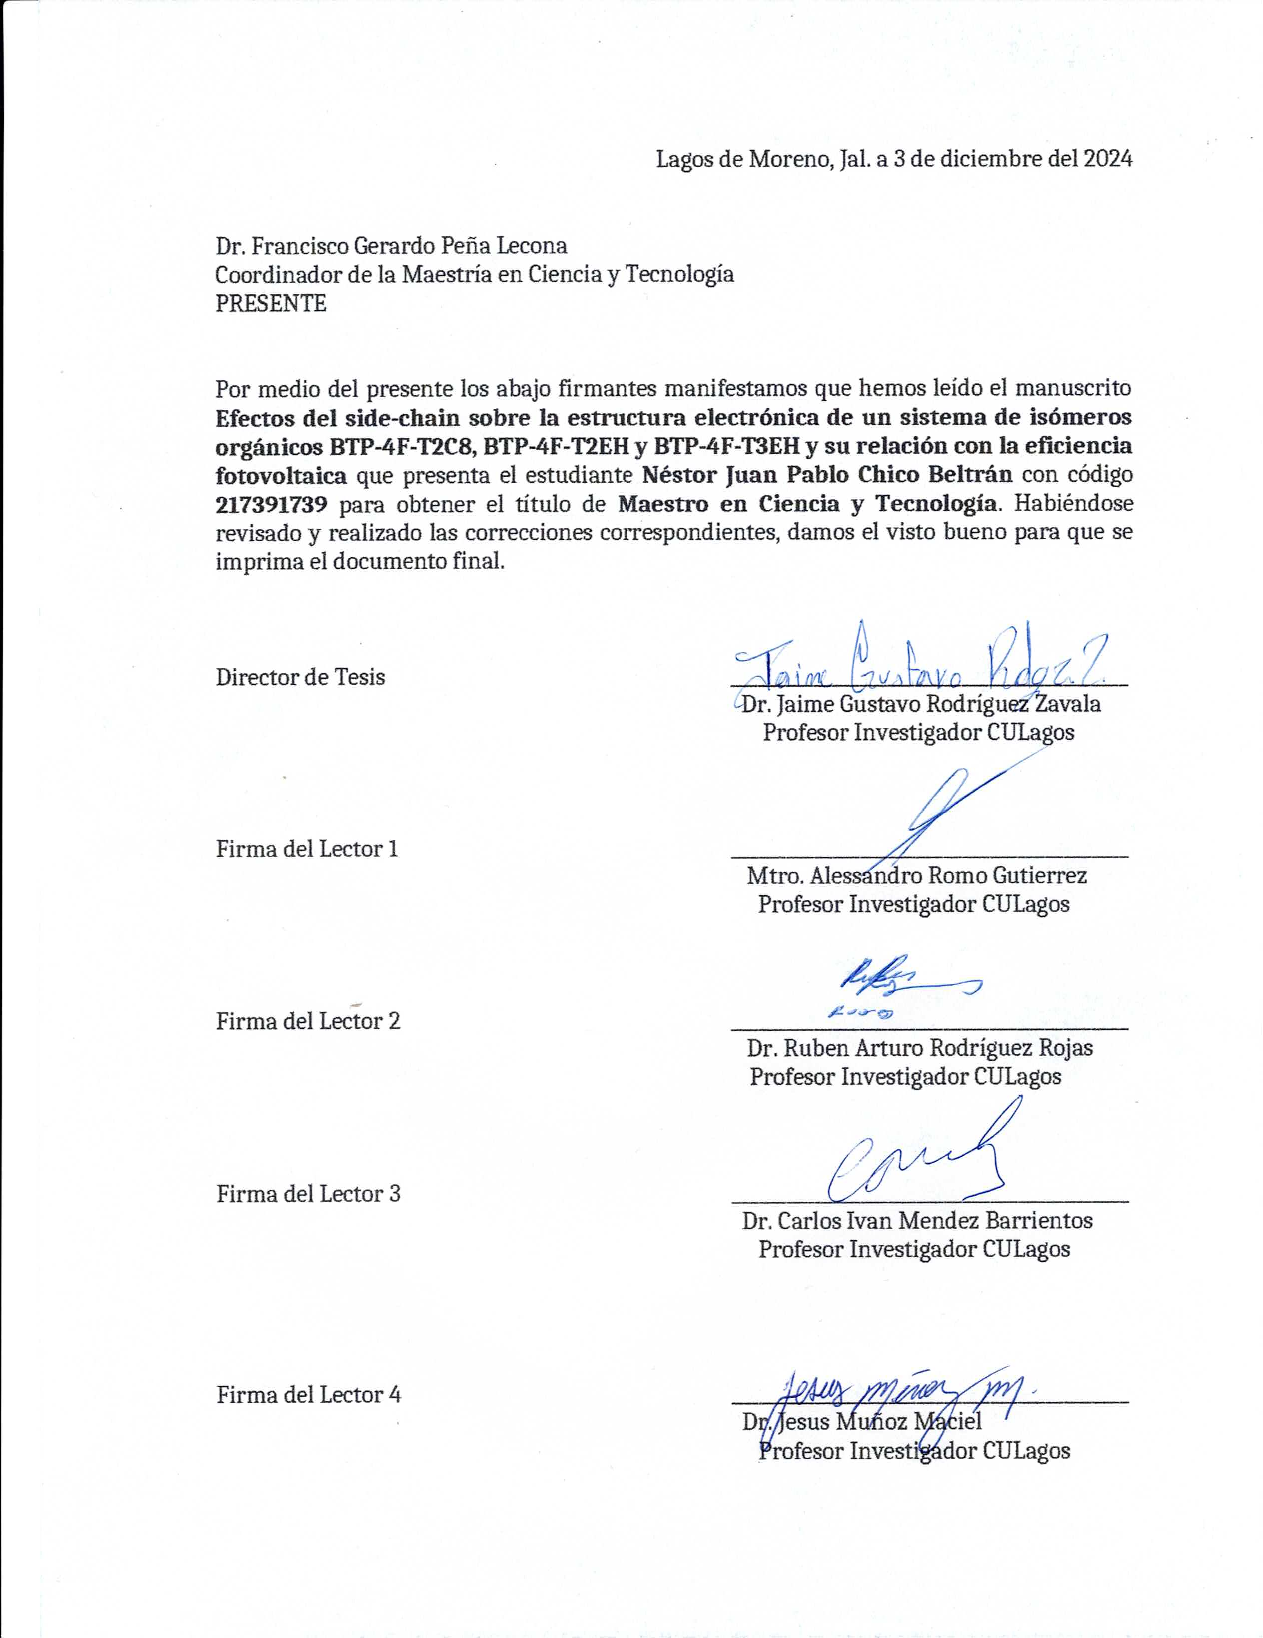
\includepdf[pages=1, offset=-1cm 0 cm]{imagenes/Portada/Vistobueno.pdf}
%                        GEOMETRÍA DE LA HOJA
% A point is approximately 1/72.27 inch, that means about 0.0138 inch or 0.3515 mm
%\setlength{\hoffset}{0 pt} % 1 Ajusta el margen izquierdo
%\setlength{\voffset}{-1 pt} % 2
%\setlength{\evensidemargin}{10 pt} % 3
%\setlength{\oddsidemargin}{10 pt} % 3
%\setlength{\topmargin}{8.534pt} % 4
%%\setlength{\headheight}{31 pt} % 5
%%\setlength{\headsep}{14pt} % 6
%%\setlength{\textheight}{640 pt} %7
%%%\setlength{\textwidth}{500 pt} % 8
%\setlength{\marginparsep}{8.5345pt} % 9
%\setlength{\marginparwidth}{28.449pt} % 10
%\setlength{\footskip}{35 pt} % 11
%----------------------------------------
\frontmatter
\hypersetup{pageanchor=true}
\renewcommand{\thepage}{\Large\roman{page}} %Con este comando puedo cambiar el tamaño de la numeración romana
\pagestyle{fancy}
\fancyhead{}
\fancyhfoffset[LE,RO]{0 cm} %Para variar el tamaño de las lineas con el texto
%%%%%%%%%%%%%%%%%%%%%%%%%%%%%%%%%%%%%%%%%%%%%%%%%%%%%%%%%%%
\renewcommand\headrulewidth{0 pt}
%La presente investigación fue elaborada en el área de Modelado Molecular y Materiales del Centro Universitario de los Lagos, ubicado en Lagos de Moreno, Jalisco, México, y estuvo auspiciada por el Consejo Nacional de Humanidades Ciencias y Tecnología (CONAHCYT).
%
%Además se desea reconocer los recursos computacionales y el soporte técnico ofrecidos por el Centro de Análisis de Datos y Supercómputo (CADS) de la Universidad de Guadalajara a través del supercomputador Leo Atrox.
%\newpage

%%% FRASES %%%
% \begin{flushright}
%\large\textbf{\textit{“¿Para qué repetir los errores antiguos \\ habiendo tantos errores nuevos que cometer?” }} \\%\addcontentsline{toc}{chapter}{Resumen}
%\vspace{2 cm} 
%\normalsize Bertrand Russell (1872-1970) Matemático británico
%\end{flushright} \newpage

%%%% DEDICATORIAS 

%\large\textbf{\textit{A mis padres}} \newpage

%%% AGRADECIMIENTOS
%\begin{center}
%\Large \centering \textit{\textbf{Agradecimientos}}
%\end{center} 
%El presente escrito ha sido elaborado gracias al apoyo inconmensurable del grupo de Modelado Molecular y Materiales, por lo que me gustaría agradecer especialmente a las siguientes personas:
%\begin{itemize}
%\item A mi director, el Dr. Jaime Gustavo Rodríguez Zavala, por su asesoría, guía, consejos y paciencia mostrada en el transcurso del posgrado. 
%\item A mi codirector, el Dr. Alessandro Romo Gutierrez, por sus valiosas y motivadoras observaciones al escrito, por su amistad y conocimientos compartidos.
%\item Dr. Zuriel Natanel Cisneros García, por atender mis dudas e inquietudes en diferentes áreas referentes al proyecto realizado en esta tesis. 
%\end{itemize}
%Además me gustaría agradecer con sumo aprecio y cariño a mis padres, quienes siempre me han apoyado en cada decisión de mi vida. A mi prometida, por brindarme su compañía incondicional, sabiduría y motivarme día a día. \\ \\
%Añado un agradecimiento final a todos y cada uno de mis amigos y compañeros del laboratorio, a mis sinodales por sus contribuciones y sugerencias al proyecto y a la Universidad de Guadalajara por brindarme la oportunidad de seguir creciendo en el ámbito académico. 


% ___________ CONTENIDO_________ 
%_________ “Sapere aude.”  ___
\tableofcontents 
%\listoffigures %Índice de figuras
%\listoftables %Índice de tablas
\newpage
%%%%%%%%%%%%%%%%%%%%%% Para hacer dos rayas en el header %%%%%%%%%%%%%%%%
\fancyhf{}
\fancyfoot[RO,LE]{\thepage}
\fancyhead[RE]{\nouppercase{\leftmark}}
\fancyhead[LO]{\nouppercase{\rightmark}}
\renewcommand\headrulewidth{0pt}
\makeatletter
\def\headrule{{\if@fancyplain\let\headrulewidth\plainheadrulewidth\fi
\hrule\@height\headrulewidth\@width\headwidth
\vskip 2pt% 2pt between lines
\hrule\@height1pt\@width\headwidth% lower line with .5pt line width
\vskip-\headrulewidth
\vskip -10pt}} %Este parametro de aqui controla que tan separadas estas las lineas del Header con respecto al texto
\makeatother
%       Color de la linea del encabezado
\let\oldheadrule\headrule% Copy \headrule into \oldheadrule
\renewcommand{\headrule}{\color{r4}\oldheadrule}% Add colour to \headrule
\renewcommand{\headrulewidth}{2.5 pt}
%\rule{\textwidth}{0.3pt} Este comando genera lineas 
%%%% Color Linea del pie de página
\let\oldfootrule
\footrule 
\renewcommand{\footrule}{\color{black}\oldfootrule}
\renewcommand{\footrulewidth}{2 pt}
%%%%%%%%%%%%%%%%%%%%    Para Cambiar Color del texto del footer %%%%%%%%%%%%%%%%%%%%%%%%%%
\makeatletter
\patchcmd{\f@nch@foot}{\rlap}{\color{Black}\rlap}{}{}
\patchcmd{\footrule}{\hrule}{\color{Black}\hrule}{}{}
%%%%% PARA el HEADER %%%%%%%%%%%%
%\patchcmd{\f@nch@head}{\rlap}{\color{red}\rlap}{}{}
%\patchcmd{\headrule}{\hrule}{\color{red}\hrule}{}{}
\makeatletter
%%%%%%%%%%%%%%%%%%%%%%%%%%%%%%%%%%%%%%%%%%%%%%%%%%%%%%%%%%%%%%%%%
\fancyhead{}
\fancyhead[L]{Resumen}
%\input{Contenido/Resumen}
\mainmatter 
\fancyfoot{}
\fancyfoot[RO,LE]{\thepage}
\fancyhead{}
%___ Para modificar solo la primera pagina de cada capitulo
\titleformat{\chapter}[display]
  {\normalfont\bfseries}{}{0pt}{\Large} % Este comando es para eliminar la aparición de "Capítulo N" en el PDF. Para emplear el formato de la tesis simplemente eliminamos la línea. 
\chapter{Introducción}
El virus del dengue (DENV) es un miembro de la familia Flaviviridae transmitido principalmente por la picadura del mosquito hembra Aedes aegypti. Este virus se clasifica en cuatro serotipos distintos (DENV-1, DENV-2, DENV-3 y DENV-4) de acuerdo con su complejo antigénico de reconocimiento, los cuales comparten entre un 65\% y un 70\% de similitud en su secuencia de aminoácidos. A nivel mundial, el DENV causa entre 50 y 100 millones de infecciones reportadas al año; una incidencia fuertemente influenciada por factores de riesgo como la urbanización acelerada, la presencia de canales o agua estancada, y el cambio climático, los cuales contribuyen directamente a la replicación y dispersión del vector. En el caso específico de México, los reportes epidemiológicos correspondientes al año 2026 continúan demostrando una alta incidencia anual y una tasa significativa de defunciones asociadas en el país.
%(1) Aspectos genéticos del virus del dengue, Genetic aspects of dengue virus, Mike Contreras1* María Angélica Rincón2, Andrea Vásquez Guillén3 Ruth Moreira4, Diana Callejas5. 
El genoma del DENV consiste en una sola cadena de ARN monocatenario de sentido positivo (+ssRNA) de aproximadamente 10.7 a 11 kb. Este genoma codifica un único marco abierto de lectura (ORF) compuesto por cerca de 3400 codones, el cual se traduce en una poliproteína que posteriormente es procesada en tres proteínas estructurales: cápside (C), de membrana (prM) y envoltura (E) y siete proteínas no estructurales: NS1, NS2A, NS2B, NS3, NS4A/2K, NS4B y NS5. Específicamente, el complejo proteico NS2B-NS3 (proteasa) juega un rol clave tanto en el procesamiento estructural de los componentes del virión como en la replicación viral. No obstante, es importante destacar que, de todos los serotipos de este virus, el serotipo 2 (DENV-2) es el más estudiado debido a su alta prevalencia y por ser el mayor causante de manifestaciones graves como la fiebre por dengue y el dengue hemorrágico \cite{contreras2021aspectos}. Desafortunadamente, a la fecha no se cuenta con vacunas con una eficacia global óptima o tratamientos antivirales aprobados universalmente, por lo que el desarrollo de inhibidores dirigidos contra las proteínas responsables de la replicación de DENV-2 es una prioridad. Entre los compuestos evaluados, se han reportado inhibidores ortostéricos (como derivados de quinoxalina) e inhibidores alostéricos (como derivados de benzofurano) con una buena concentración inhibitoria in vitro y un gran impacto sobre sitios específicos; sin embargo, limitaciones farmacocinéticas o de toxicidad han impedido que avancen hacia fases clínicas. Por lo tanto, el diseño de nuevos inhibidores contra la proteasa NS2B-NS3 (utilizando como diana la estructura de la proteína en conformación inactiva-abierta, identificada con el código PDB: 2FOM) representa una estrategia terapéutica prometedora debido a que al estabilizar el estado inactivo-abierto se impide que la enzima realice el cambio conformacional hacia su forma cerrada y catalíticamente activa, bloqueando así el procesamiento de la poliproteína viral. 

Como alternativa en el desarrollo de fármacos, en este estudio se reporta el análisis de nanoestructuras de carbono. Debido a la versatilidad de los átomos de carbono para adoptar diferentes hibridaciones orbitales, estos pueden formar enlaces direccionados sumamente estables y dar origen a diversas estructuras alotrópicas. Una de las más destacadas es el fulereno, una estructura molecular compuesta únicamente por carbono que se presenta en distintos tamaños, como C\textsubscript{20}, C\textsubscript{60}, C\textsubscript{70} y C\textsubscript{76}. La más conocida y estudiada de estas formas es el C\textsubscript{60} (o buckminsterfulereno), constituido por 20 hexágonos y 12 pentágonos. Esta molécula cuenta con dos tipos de enlaces: los enlaces [6,6] con una distancia de 1.38 Å, y los enlaces [5,6] con una distancia de 1.45 Å. \cite{fajardo2012dengue} El descubrimiento de estas nuevas formas de carbono otorgó a los investigadores Harold W. Kroto, Robert F. Curl Jr. y Richard E. Smalley el Premio Nobel de Química en 1996.

A pesar de sus notables propiedades físicas y electrónicas, el C\textsubscript{60} presenta una limitación crítica para su uso biomédico: su baja solubilidad en medios acuosos. Para superar este inconveniente, se ha propuesto la funcionalización del fulereno mediante la adición de aminoácidos. Numerosos estudios de aductos de C\textsubscript{60} modificados con L-metionina, L-hidroxiprolina y L-arginina han demostrado una pronunciada actividad biológica como agentes antioxidantes, antimicrobianos, antivirales, antitumorales, neuroprotectores, membranotrópicos y fotodinámicos, actuando incluso como radioprotectores e inductores de la apoptosis. Específicamente, el aducto de C\textsubscript{60} funcionalizado con cuatro moléculas de glicina ha sido reportado con una notable actividad antioxidante, propiedades de fotoprotección y una excelente hemocompatibilidad, logrando además el parámetro más importante: una solubilidad aceptable para aplicaciones en sistemas biológicos \cite{krishna2024dengue}. Así, estos aductos sirven como andamios moleculares versátiles para el desarrollo de nuevos materiales con fines médicos y terapéuticos contra diversas enfermedades.

Dado lo anterior, el presente estudio teórico-computacional consiste en la determinación de una serie de parámetros estructurales y energéticos que forman parte de la caracterización del aducto C\textsubscript{60}-glicina (modificado con cuatro moléculas de glicina). Mediante una metodología computacional, este trabajo tiene como objetivo evaluar y analizar el comportamiento, la afinidad y la actividad de este aducto como un inhibidor potencial contra la proteasa NS2B-NS3 del virus del dengue serotipo 2 (DENV-2), empleando para ello el modelo estructural en conformación abierta-inactiva (PDB: 2FOM), debido a que esta conformación impide que la proteína adopte su estructura activa-cerrada necesaria para llevar a cabo la catálisis proteolítica. 




\chapter{Resumen}
En el presente trabajo se evaluó el potencial del fulereno C\textsubscript{60} funcionalizado con cuatro moléculas de glicina, C\textsubscript{60}(Gly)\textsubscript{4}, como posible inhibidor de la proteasa NS2B-NS3 del virus del dengue serotipo 2 (DENV-2). La elección de este sistema se basa en el interés por los derivados de fulereno con actividad antioxidante y en que su funcionalización con aminoácidos favorece su solubilidad en medios biológicos.

La caracterización electrónica, basada en la teoría del funcional de la densidad (DFT) y en las funciones de Fukui, permitió analizar la distribución de los grupos de glicina alrededor de la jaula del fulereno y los cambios asociados en su estructura electrónica. Las simulaciones de acoplamiento molecular mostraron afinidades favorables en regiones reportadas como sitios alostéricos y ortostéricos de la proteína. El análisis estructural identificó interacciones intermoleculares, entre ellas puentes de hidrógeno e interacciones de van der Waals. La presencia de los grupos de glicina modificó el potencial electrostático del aducto y su interacción con el entorno proteico.

La simulación de dinámica molecular del complejo proteína--aducto mostró estabilidad estructural durante el periodo analizado de 100 ns. Asimismo, la caracterización electrónica indicó una mayor facilidad para donar electrones respecto al fulereno sin funcionalizar. Estos resultados aportan información sobre el comportamiento del sistema en las condiciones simuladas y respaldan su estudio como candidato a inhibidor. Su actividad antiviral y su capacidad antioxidante requieren confirmación experimental.

\titleformat{\chapter}[display]
  {\normalfont\bfseries}{}{0pt}{\Large} % Este comando es para eliminar la aparición de "Capítulo N" en el PDF. Para emplear el formato de la tesis simplemente eliminamos la línea. 
\chapter{Antecedentes}
El dengue es la enfermedad viral transmitida por vectores de más rápida expansión en el mundo. Actualmente, se estima que más de la mitad de la población global se encuentra en riesgo de infección. El agente causal es el virus del dengue (DENV), un arbovirus perteneciente a la familia \textit{Flaviviridae} compuesto por cuatro serotipos distintos (DENV-1 a DENV-4). La infección por un serotipo otorga inmunidad permanente contra ese mismo tipo, pero solo una protección temporal contra los demás. Transmitido principalmente por hembras infectadas del género \textit{Aedes} (\textit{Aedes aegypti} y \textit{Aedes albopictus}), la incidencia del DENV aumentó un 85\% entre 1990 y 2019. Hoy en día, genera entre 50 y 100 millones de casos sintomáticos al año, de un total de hasta 390 millones de infecciones y cerca de 14\,000 muertes anuales. 

\textit{Aedes aegypti} representa el principal vector en el hemisferio occidental debido a su gran adaptación a entornos urbanos y recipientes domésticos. La combinación de esta presencia vectorial con el rápido crecimiento demográfico ha provocado un incremento constante en la morbilidad. De acuerdo con la Organización Panamericana de la Salud (OPS), al cierre de 2019 se notificaron más de 3.1 millones de casos en América Latina. Asimismo, los estudios estiman que el DENV ocasiona cerca de 500\,000 cuadros de dengue grave al año y un impacto económico de 39\,000 millones de dólares en costos directos e indirectos \cite{contreras2021aspectos}.

La frecuencia e intensidad de los brotes epidémicos se ven favorecidas por la alta densidad poblacional urbana, el acceso deficiente a agua potable y el incremento de los viajes internacionales. Según la OMS, entre 2\,700 y 3\,000 millones de personas residen en áreas aptas para la transmisión vectorial \cite{krishna2024dengue}. Por otro lado, los factores climáticos ejercen una influencia determinante. El aumento sostenido de la temperatura acelera el desarrollo del vector, acorta el periodo de incubación del virus y eleva la frecuencia de picaduras. A su vez, las lluvias incrementan los criaderos disponibles, estructurando nichos ecológicos de transmisión dinámicos y cambiantes \cite{mendoza2025spatial} \newpage 

\section{Dinámica Evolutiva del Serotipo 2 (DENV-2)}
El serotipo 2 del virus del dengue (DENV-2) posee una amplia diversidad genética y filogenética. Se clasifica en cinco genotipos endémicos y epidémicos de carácter no selvático: Americano (GI), Cosmopolita (GII), Asiático-Americano (GIII), Asiático-II (GIV) y Asiático-I (GV). Históricamente, el genotipo Americano (DENV-2-GI) fue la primera variante registrada en las Américas a mediados de la década de 1940. Sin embargo, a partir de los años 1980 fue desplazado casi por completo por el genotipo Asiático-Americano (DENV-2-GIII). Tras esta sustitución, la variante ancestral GI dejó de detectarse en los registros epidemiológicos \cite{allicock2012phylogeography}.

%(44) En el contexto sudamericano, Brasil representa un escenario complejo de hiperendemicidad y evolución viral. Tras la llegada del genotipo Asiático-Americano (GIII) en la década de 1990 —impulsada por migraciones desde el Caribe y el norte de América del Sur—, la cocirculación constante de los cuatro serotipos se ha relacionado con un incremento en la virulencia clínica y en la mortalidad hospitalaria. (44)
Por otra parte, la primera detección del genotipo Cosmopolita en América se reportó a finales de los años 1990 en la Península de Yucatán, México. Sin embargo, en su momento existieron limitaciones técnicas para obtener una caracterización clínica detallada de dichos aislados \cite{hou2024fullerene}.

En años recientes, la emergencia e introducción del genotipo Cosmopolita (DENV-2-GII) en el continente americano se ha convertido en un acontecimiento de gran relevancia epidemiológica. Las primeras detecciones registradas en 2021 en Brasil (Goiás y Acre), respaldadas por análisis filogenéticos, sugieren que este linaje proviene de un brote epidémico previo ocurrido en Perú en 2019 \cite{amorim2023emergence}. Es importante señalar que el genotipo DENV-2-GII posee la mayor dispersión geográfica a nivel mundial (con presencia en Asia-Pacífico, Oriente Medio, África y Oceanía). Por esta razón, su afianzamiento en América representa un riesgo significativo para la salud pública al alterar los patrones de transmisión y aumentar la carga de la enfermedad \cite{hou2024fullerene}. 
\section{Comportamiento Epidemiológico en México}
 En México, la situación epidemiológica se caracteriza por la circulación endémica de los cuatro serotipos del DENV en 29 entidades federativas. Esta dinámica afecta a más de 50 millones de habitantes. La cocirculación simultánea de dos o más serotipos en diversas regiones configura un estado de hiperendemicidad. Esta condición incrementa el riesgo de desarrollar formas severas de la enfermedad (como el dengue hemorrágico) debido a mecanismos de potenciación inmunológica por anticuerpos. Al cierre del año epidémico (semana epidemiológica 52), se registraron en el país 69\,910 casos probables y 15\,578 casos confirmados. De estos últimos, 10\,970 correspondieron a dengue no grave y 4\,608 a dengue con signos de alarma o dengue grave, mostrando un comportamiento fluctuante entre años  \textbf{véase el Cuadro \ref{tab:dengue_2025_2026}} \cite{fajardo2012dengue}.

Para monitorear el impacto de estos linajes en el país, la Secretaría de Salud realiza un seguimiento semanal mediante el Sistema Especial de Vigilancia Epidemiológica de Dengue (SINAVE). Como se muestra en la \textbf{Figura \ref{Fig:1.1}}, los análisis por RT-PCR en tiempo real reflejan la tasa de incidencia por cada 100,000 habitantes y la cocirculación de serotipos por entidad federativa. En este periodo, la mayor carga se registró en Sonora (31.97), destacando un predominio del serotipo DENV-3 junto con focos activos de DENV-2. Cabe señalar que los reportes del SINAVE identifican los estados con circulación activa de DENV-2. Sin embargo, la confirmación sobre la llegada y expansión específica del genotipo Cosmopolita requiere de un seguimiento genómico complementario en dichos focos epidémicos.

\begin{figure}[H]
  \centering
  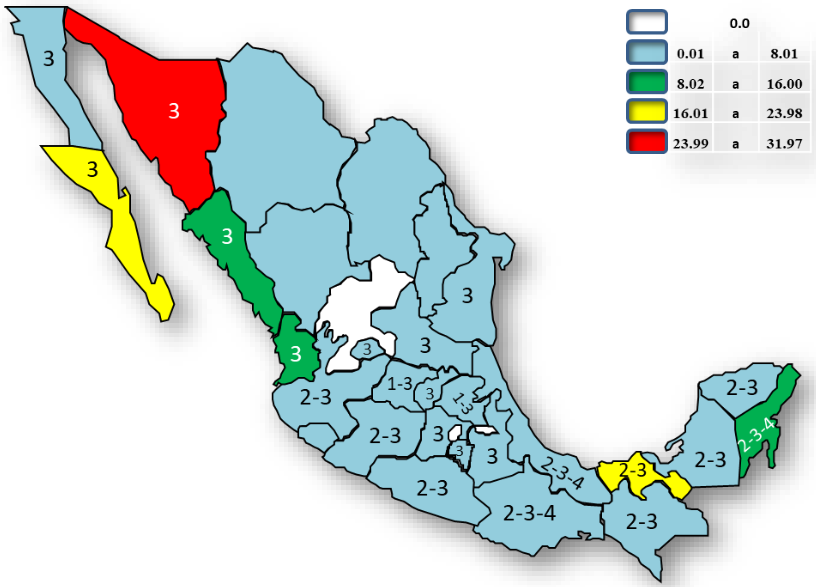
\includegraphics[width=9cm]{imagenes/Ant/mexico.png}
  \caption{Relaciones de similitud de secuencia y conservación estructural entre los serotipos del DENV \cite{arias1993dengue}.}
  \label{Fig:1.1}
\end{figure}


\begin{table}[htbp]
    \centering
    \caption{Comparativo de casos probables y confirmados de dengue en México (Período 2025--2026).}
    \label{tab:dengue_2025_2026}
    \small
    \begin{tabular}{|c|c|c|c|c|c|c|c|c|c|}
        \hline
        \multicolumn{2}{|c|}{\textbf{PROBABLES}} & \multicolumn{8}{c|}{\textbf{CONFIRMADOS}} \\
        \hline
        \textbf{2025} & \textbf{2026} & \multicolumn{4}{c|}{\textbf{2025}} & \multicolumn{4}{c|}{\textbf{2026}} \\
        \cline{3-10}
        & & \textbf{DNG} & \textbf{DCSA} & \textbf{DG} & \textbf{Total} & \textbf{DNG} & \textbf{DCSA} & \textbf{DG} & \textbf{Total} \\
        \hline
        49\,085 & 29\,977 & 2\,192 & 2\,167 & 175 & 2\,342 & 1\,230 & 1\,504 & 113 & 1\,617 \\
        \hline
    \end{tabular}
    \\[2mm]
    \raggedright \scriptsize \textbf{Abreviaturas:} \textbf{DNG:} Dengue No Grave; \textbf{DCSA:} Dengue Con Signos de Alarma; \textbf{DG:} Dengue Grave; \textbf{Total:} DCSA + DG.
\end{table} 
\subsection{Estructura Genómica del Virus del Dengue (DENV)}
La caracterización genómica de cepas representativas de los cuatro serotipos del virus del dengue (DENV-1 a DENV-4) ha permitido comprender mejor la arquitectura viral y sus relaciones filogenéticas \textbf{véase la Figura \ref{fig:denv_secuencia}}. Los cuatro serotipos comparten aproximadamente un 70\% de identidad en su secuencia de aminoácidos. Asimismo, presentan un 50\% de homología con otros miembros representativos del género \textit{Flavivirus}, como el virus de la fiebre amarilla y el virus de la encefalitis japonesa \cite{arias1993dengue}.

\begin{figure}[H]
  \centering
  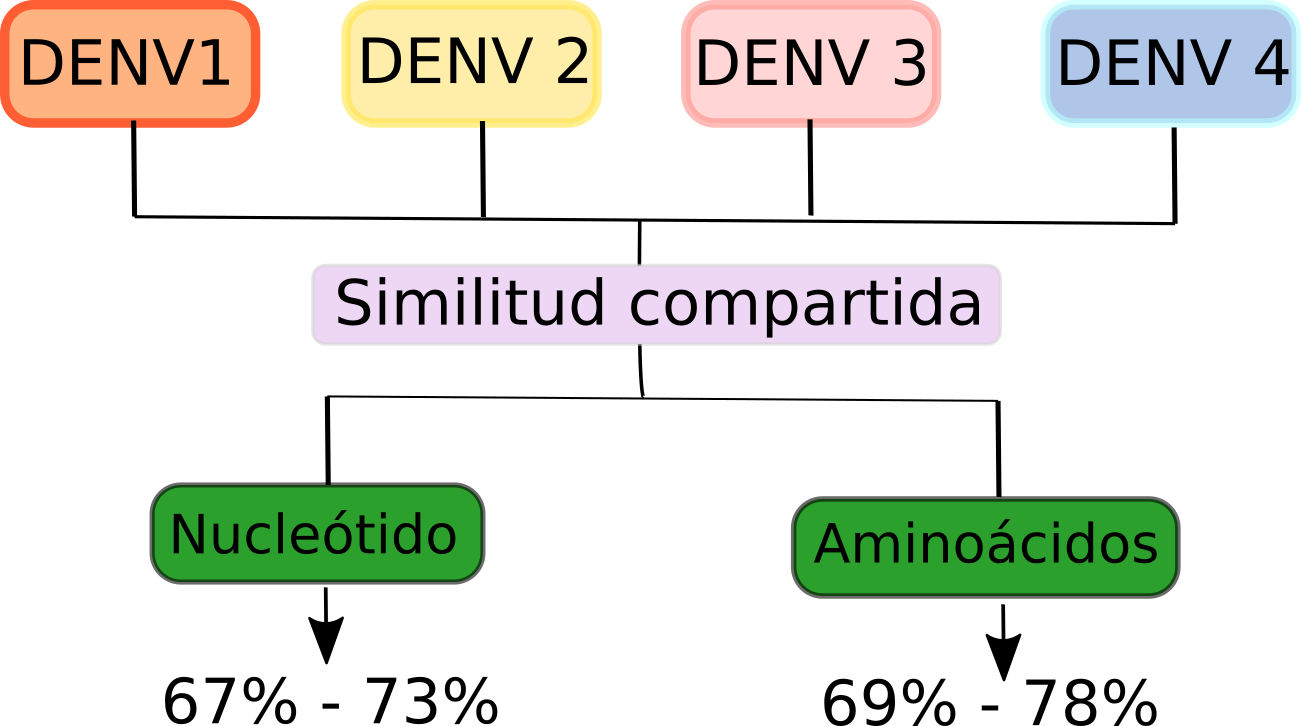
\includegraphics[width=9cm]{imagenes/Ant/diagrama-1.png}
  \caption{Relaciones de similitud de secuencia entre serotipos del DENV.}
  \label{fig:denv_secuencia}
\end{figure}

El genoma del virus del dengue está constituido por una molécula de ARN monocatenario de sentido positivo (+ssRNA), perteneciente a la familia \textit{Flaviviridae} \cite{sinha2024dengue}. Con una extensión aproximada de 11 kb, posee un único marco de lectura abierto (ORF) flanqueado por dos regiones no traducidas (5' UTR y 3' UTR). El extremo 5' UTR presenta una estructura de capuchón tipo 1 (m7GpppAmp). Por su parte, el extremo 3' UTR carece de la cola poli(A) convencional \cite{krishna2024dengue}.

La partícula viral madura posee una morfología esférica de aproximadamente 50 nm de diámetro. Esta estructura cuenta con una envoltura lipídica que rodea a la nucleocápside, dentro de la cual se empaqueta el ARN genómico \textbf{véase la Figura \ref{fig:denv_genoma}} \cite{dhole2024host}. Al ingresar a la célula hospedera, el ARN viral se traduce en la membrana del retículo endoplásmico (RE) en una poliproteína única. Posteriormente, esta cadena es procesada proteolíticamente para dar origen a tres proteínas estructurales —cápside (C), precursor de membrana/membrana (prM/M) y envoltura (E)— y a siete proteínas no estructurales (NS1, NS2A, NS2B, NS3, NS4A, NS4B y NS5) \cite{sinha2024dengue}.

\begin{figure}[H]
  \centering
  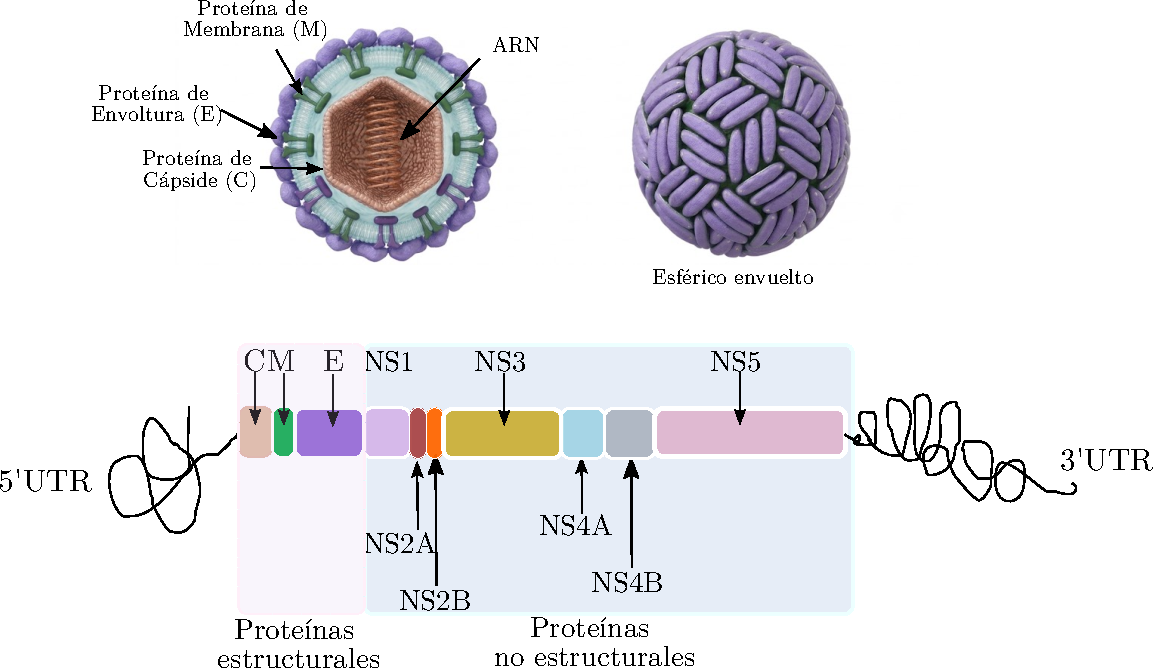
\includegraphics[width=13cm]{imagenes/Ant/genes.pdf}
  \caption{Organización genómica y procesamiento de la poliproteína del DENV.}
  \label{fig:denv_genoma}
\end{figure}

El procesamiento proteolítico co- y post-traduccional de la poliproteína está coordinado por la proteasa viral NS2B-NS3 en el citoplasma, y por proteasas del huésped (señalasa y furina) en el lumen del RE. Las glicoproteínas E y M se organizan en la superficie de la bicapa lipídica con simetría icosaédrica. Durante el tránsito del virión inmaduro por la Red \textit{Trans}-Golgi (TGN), el pH ácido induce un cambio conformacional en la proteína E. Este cambio expone el sitio de escisión de prM para la acción de la furina. Posteriormente, la exocitosis hacia el espacio extracelular (pH $\approx 7.0$) provoca la liberación del péptido \textit{pr}. Este proceso permite la transición del virión desde una forma inmadura ("rugosa") hacia una partícula madura e infecciosa. Por su parte, las proteínas no estructurales cumplen funciones clave: NS1 evade la respuesta inmune al inhibir la activación del sistema del complemento, mientras que NS2A y NS4B participan en el ensamblaje del complejo de replicación \cite{pourzangiabadi2025dengue}.

\section{Arquitectura Molecular del Complejo Proteico NS2B-NS3}
La proteína no estructural 3 (NS3) es una enzima multifuncional constituida por dos dominios bien definidos. El dominio N-terminal actúa como una serina proteasa similar a la quimiotripsina, mientras que el dominio C-terminal presenta actividades de ARN helicasa, NTPasa y ARN 5'-trifosfatasa. Para llevar a cabo su función proteolítica, NS3 requiere de forma obligatoria interactuar en \textit{cis} o \textit{trans} con la proteína transmembrana NS2B, la cual actúa como su cofactor funcional \cite{diosa2020role}.

El dominio de serina proteasa comprende los primeros 180 aminoácidos N-terminales de NS3, de un total de 618 residuos. La expresión aislada de este dominio (NS3pro) o de la proteína completa (NS3 FL) produce agregados insolubles e inactivos. Para solubilizar y activar a NS3pro, se requiere la región hidrofílica central de NS2B (residuos 49 al 95). Mediante ingeniería de proteínas, la unión del segmento de NS2B con NS3pro a través de un enlazador flexible (Gly4-Ser-Gly4) permite obtener un complejo soluble y catalíticamente activo (NS2B-NS3pro). Al respecto, estudios estructurales de Erbel et al. (2006) demostraron que los residuos N-terminales 49–66 de NS2B actúan como una chaperona molecular. Esta región se inserta como una hebra $\beta$ en el barril N-terminal de NS3, protegiendo sus residuos hidrofóbicos de la exposición al solvente \cite{lescar2008towards}.

Sin embargo, la región N-terminal de NS2B no es suficiente para la actividad catalítica. Los residuos C-terminales del cofactor (Glu66–Leu95) son indispensables para estructurar el sitio activo. En esta zona, los aminoácidos Glu67–Asp76 forman las hebras $\beta_2$ y $\beta_3$. Por su parte, los residuos Arg78–Leu87 constituyen un bucle $\beta$ que abraza el barril C-terminal de NS3 \textbf{véase la Figura \ref{fig:ns2b_ns3_abierta}} . Esta disposición posiciona aminoácidos clave (Gly151, Gly153 y Tyr161) para el reconocimiento del sustrato e interviene directamente en la conformación de los bolsillos S2 y S3 \cite{erbel2006structural}. En consecuencia, el cofactor NS2B ejerce un doble papel regulador sobre NS3. Por un lado, estabiliza el plegamiento terciario del dominio proteasa. Por el otro, participa de forma directa en la conformación de la cavidad catalítica, permitiendo el reconocimiento de residuos básicos (Arg/Lys) en las posiciones P1 y P2 del sustrato \cite{luo2015flavivirus}.

Análisis estructurales comparativos revelan que, en ausencia de NS3pro, el cofactor NS2B libre se encuentra desordenado en solución. Al asociarse, la región N-terminal del cofactor forma un complejo estable con el dominio proteasa, mientras que su extremo C-terminal mantiene una alta flexibilidad. Estudios de cristalografía en estado \textit{apo} (libre de ligando) de flavivirus como el WNV y el DENV muestran que la proteasa existe principalmente en una ``conformación abierta'' inactiva. En este estado, la región C-terminal de NS2B se orienta hacia el solvente y permanece alejada del centro catalítico. Esta disposición espacial impide la catálisis, ya que se necesita la interacción directa de los residuos C-terminales del cofactor para organizar funcionalmente el sitio activo \cite{li2020insights}.

\begin{figure}[H]
  \centering
  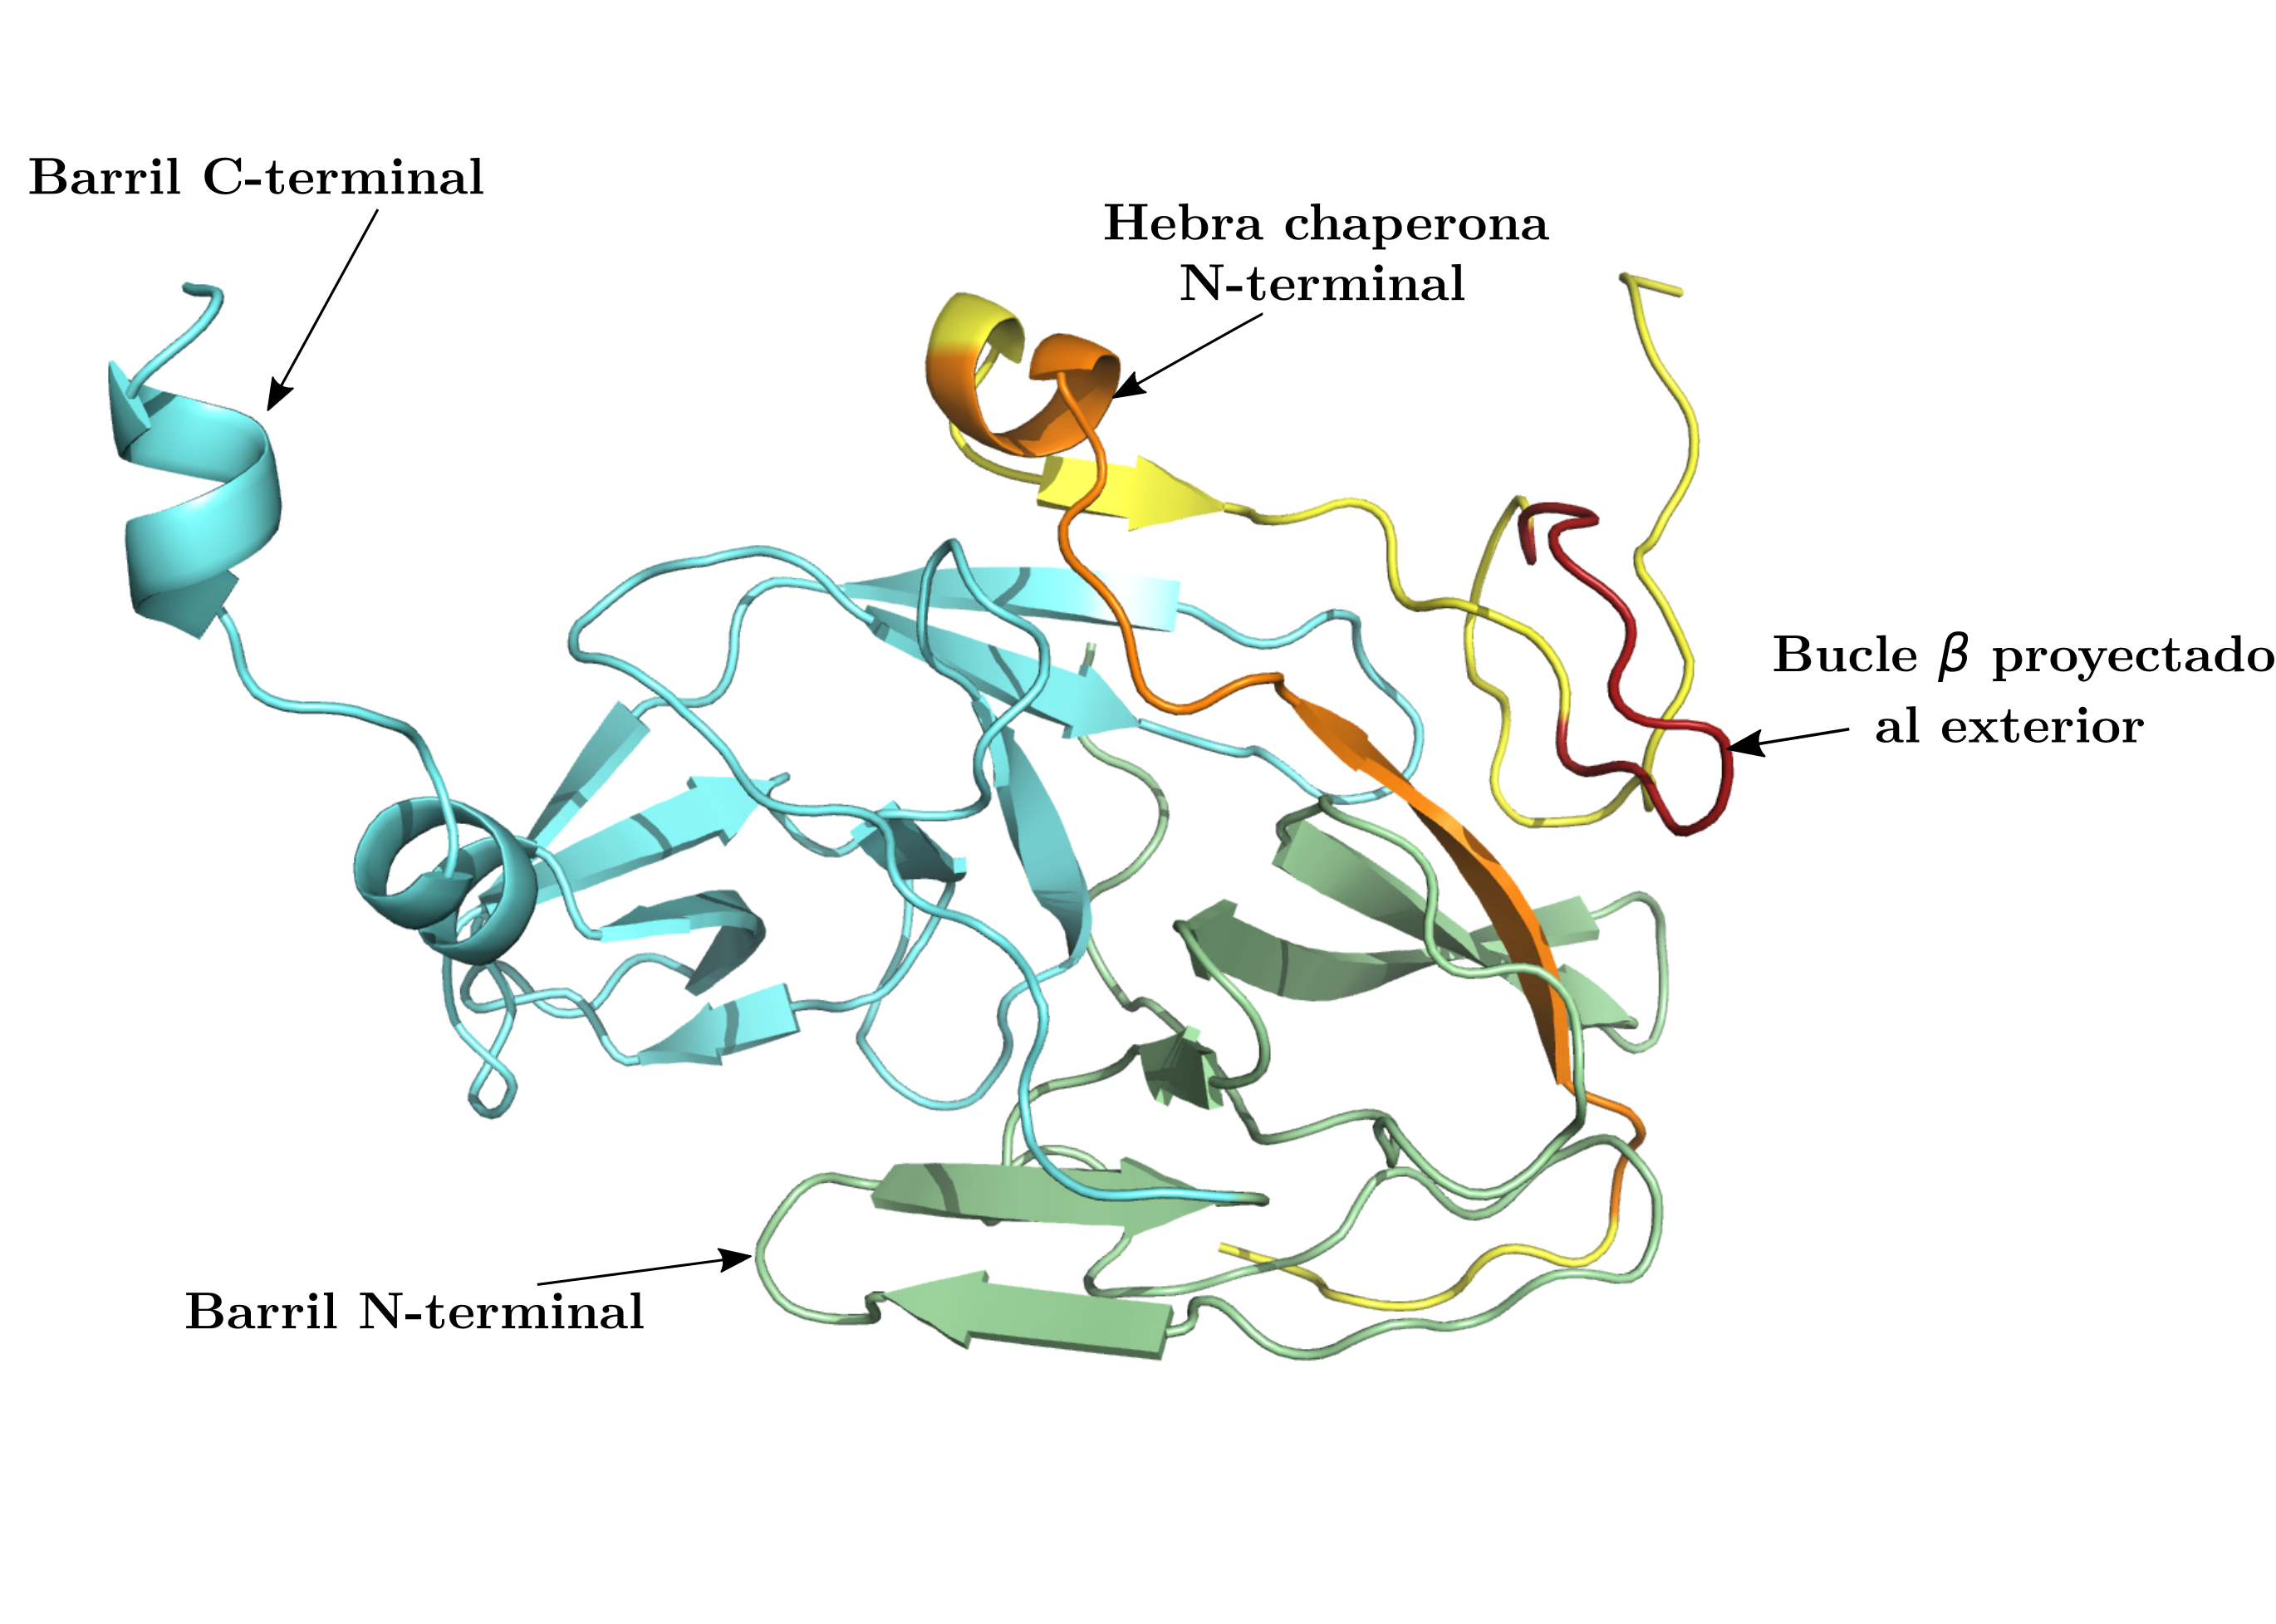
\includegraphics[width=13cm]{imagenes/Ant/2FOM-bucles.png}
  \caption{Estructura cristalina de la proteasa NS2B-NS3 del DENV-2 en conformación abierta (PDB ID: 2FOM). Representación tridimensional en cinta del complejo en ausencia de ligando. Se destacan los dos barriles $\beta$ (N-terminal y C-terminal) que forman el núcleo catalítico de NS3, la hebra chaperona N-terminal del cofactor NS2B anclada a NS3 y el bucle $\beta$ C-terminal proyectado hacia el exterior, característico del estado inactivo o desacoplado \cite{li2020insights,de2011binding,maus2021sar}.}
  \label{fig:ns2b_ns3_abierta}
\end{figure}
La transición desde la conformación abierta inactiva hacia la ``conformación cerrada'' activa ocurre mediante un reordenamiento conformacional. Este cambio es impulsado por la unión del sustrato o de un inhibidor ortostérico. Durante el proceso, el extremo C-terminal de NS2B se pliega alrededor de NS3pro, formando una horquilla $\beta$ que cubre la cavidad catalítica. Este cierre conformacional empaqueta los residuos clave del cofactor contra el dominio catalítico. De este modo, se fija la estructura tridimensional de los subsitios S2 a S4 y se activa la capacidad funcional del sitio catalítico \cite{li2020insights,de2011binding,maus2021sar}.
Es importante destacar que la conformación abierta observada en la estructura cristalina en estado \textit{apo} (PDB ID: 2FOM) ha sido objeto de debate en la literatura. Mientras que los estudios de cristalografía iniciales sugerían que la proteasa libre adopta preferentemente esta disposición inactiva, investigaciones de Resonancia Magnética Nuclear (RMN) en solución y análisis dinámicos recientes \cite{li2020insights,nitsche2023targeting} revelan que el complejo proteico experimenta una dinámica conformacional altamente fluida. En ausencia de ligando, la región C-terminal del cofactor NS2B oscila libremente entre un estado desacoplado y la conformación cerrada en un equilibrio termodinámico rápido, siendo la conformación cerrada la predominantemente poblada en condiciones fisiológicas. La cristalización de la forma abierta suele verse favorecida por empaquetamiento cristalino o por el uso de enlazadores artificiales de poliglicina ($G_4SG_4$). Por consiguiente, la captura de la estructura cerrada activa mediante RMN (PDB ID: 2M9P; \textbf{véase la Figura \ref{fig:ns2b_ns3_comparacion}} evidencia que el dominio C-terminal de NS2B no solo actúa como un elemento estructural indispensable, sino como un regulador alostérico dinámico clave para la catálisis.



\begin{figure}[H]
  \centering
  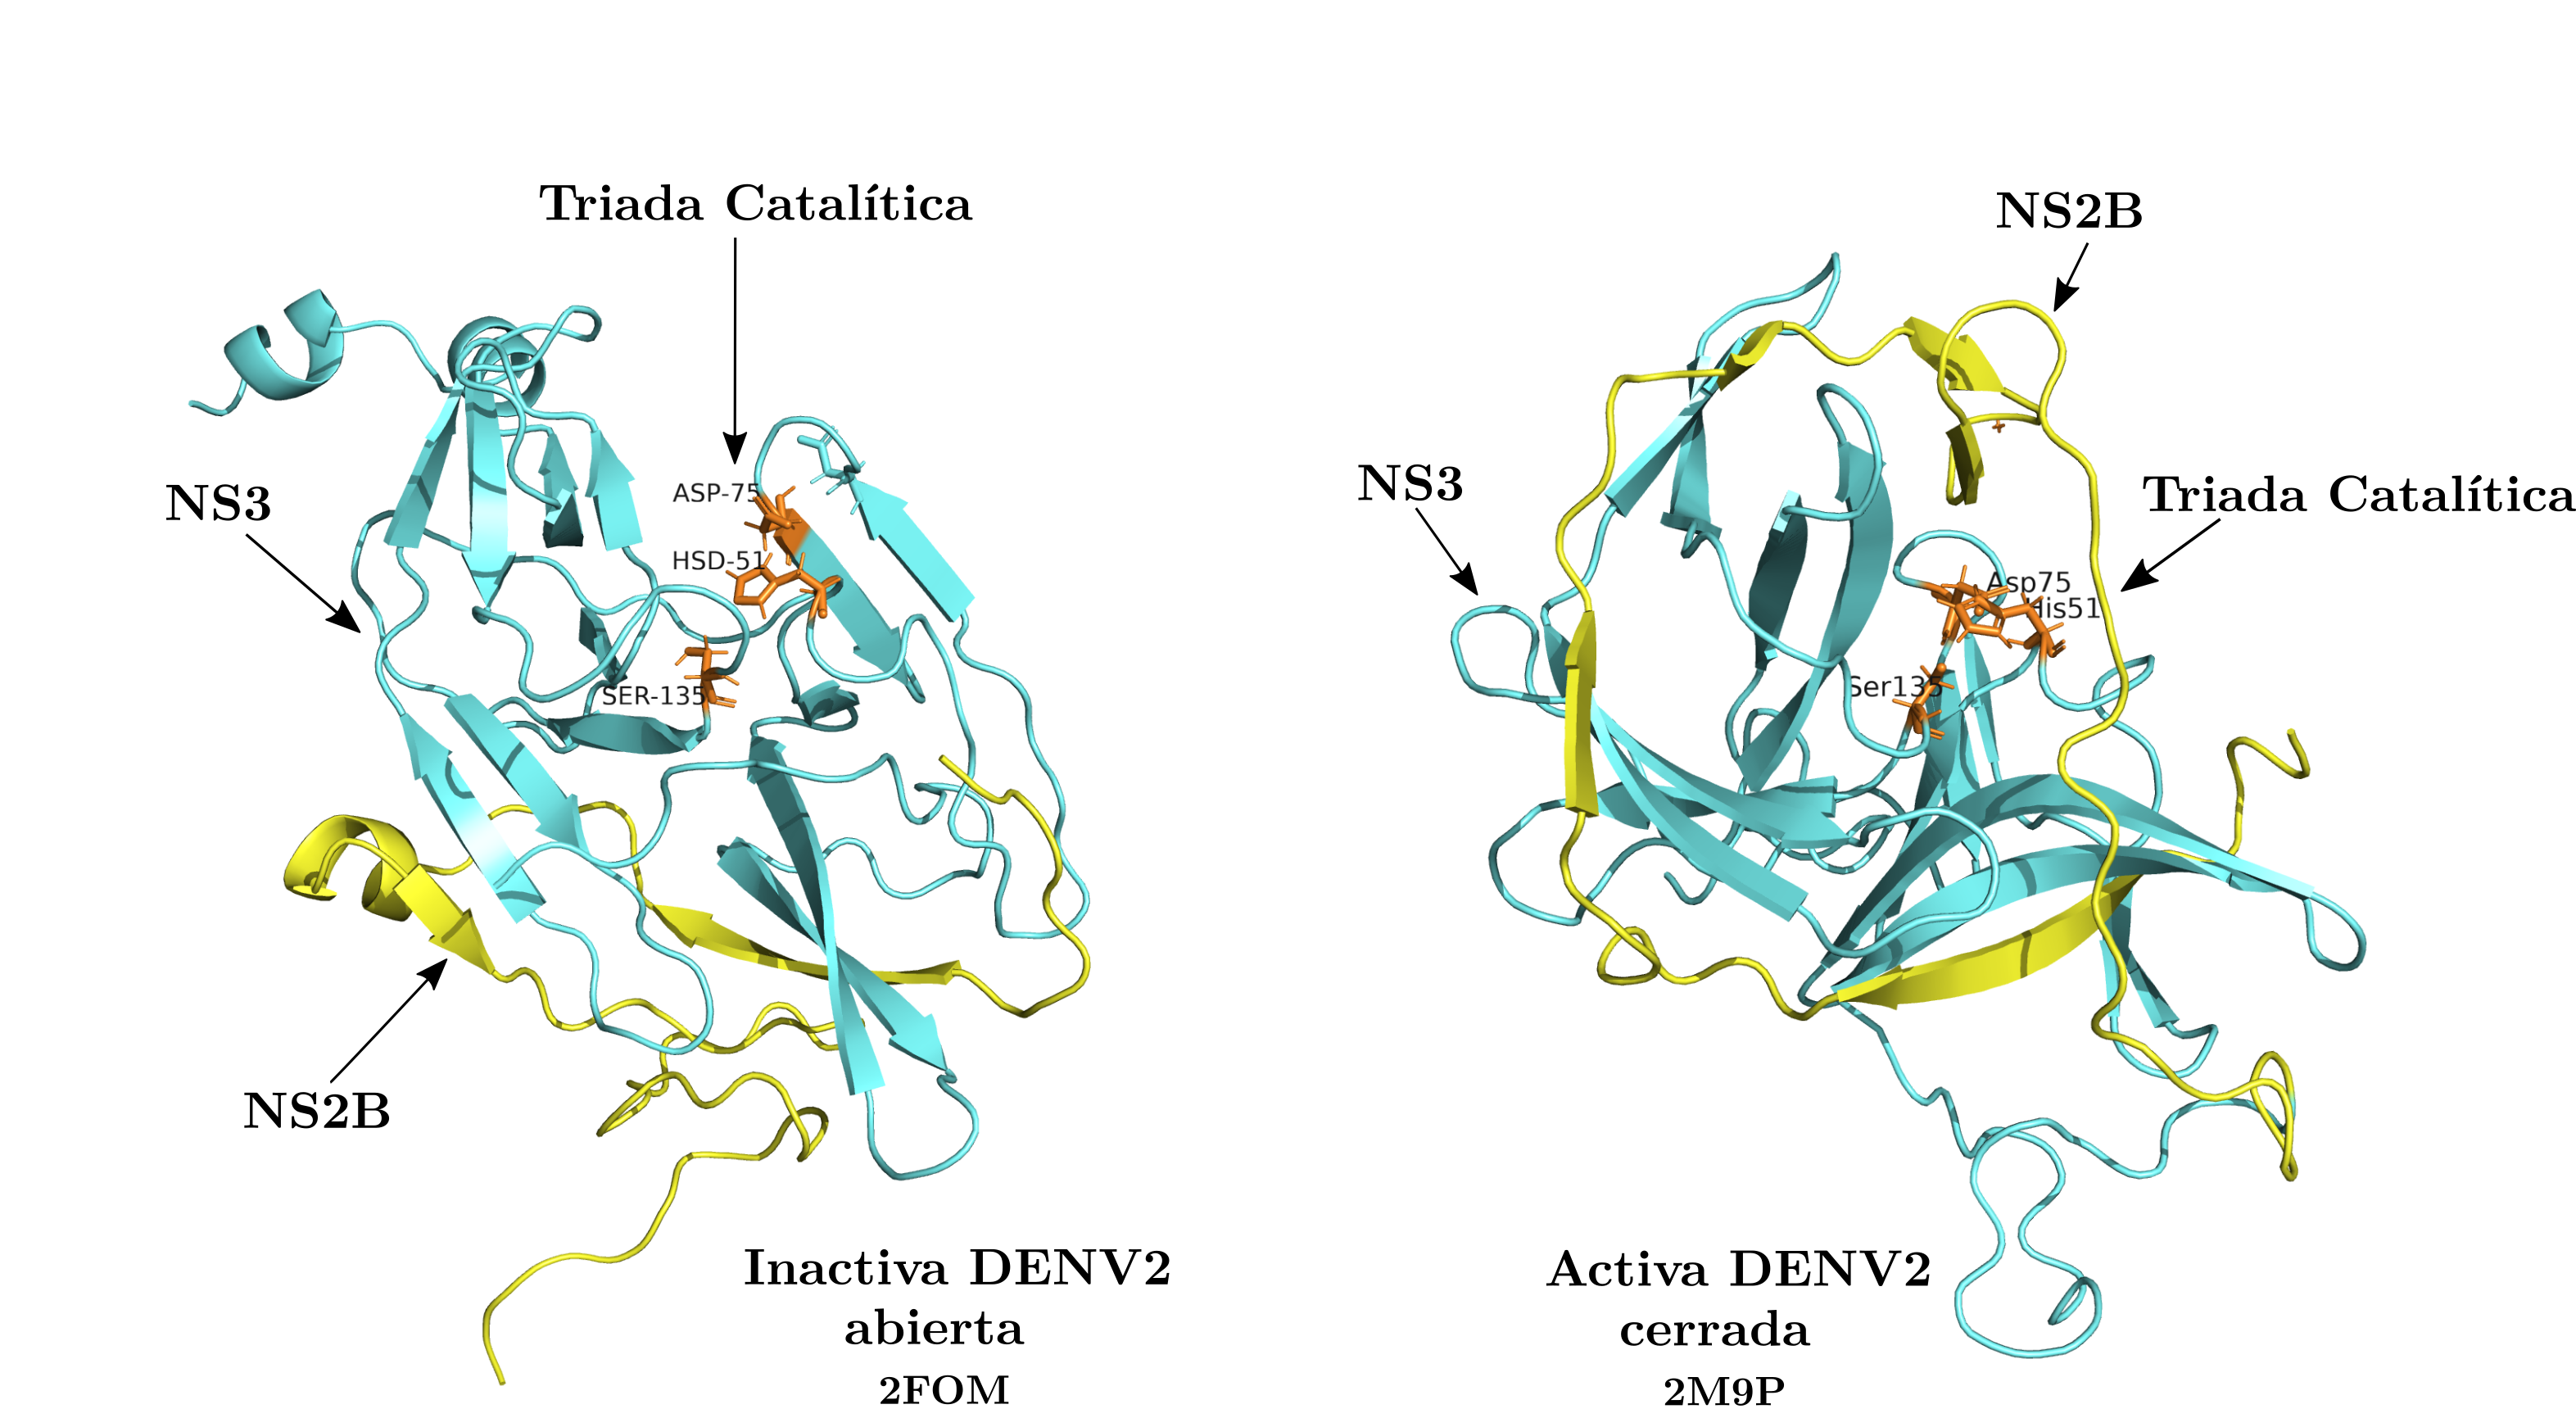
\includegraphics[width=16cm]{imagenes/Ant/2FOM-conformaciones.png}
  \caption{Comparación conformacional del complejo proteasa NS2B-NS3pro del virus del dengue serotipo 2 (DENV-2). \textbf{Izquierda:} Conformación abierta e inactiva en estado \textit{apo} (PDB ID: 2FOM). En esta forma, la región C-terminal del cofactor NS2B (amarillo) permanece desacoplada del dominio catalítico NS3 (cian). \textbf{Derecha:} Conformación cerrada y activa (PDB ID: 2M9P), la cual muestra el reordenamiento del bucle C-terminal de NS2B alrededor de NS3 para estructurar el sitio activo. En ambas estructuras se resaltan en bastones (\textit{sticks}) los residuos de la tríada catalítica (His51, Asp75 y Ser135) \cite{li2020insights,de2011binding,maus2021sar}.}
  \label{fig:ns2b_ns3_comparacion}
\end{figure}


\section{Mecanismo Catalítico e Inhibición Enzimática}
La maquinaria catalítica de la proteasa viral está formada por la tríada clásica de serina proteasas (His51, Asp75 y Ser135). Esta estructura se encuentra altamente conservada en la familia \textit{Flaviviridae}. Por su parte, la cavidad catalítica exhibe un potencial electrostático principalmente negativo. Esta propiedad es esencial, ya que condiciona la especificidad del sustrato al favorecer interacciones iónicas hacia residuos cargados positivamente (Lys y Arg) en los sitios de corte de la poliproteína \cite{li2020insights}.

La proteasa NS2B-NS3 constituye un blanco farmacológico primario debido a su papel en la replicación viral y en el procesamiento de factores inmunomoduladores del huésped. Su sitio activo se compone de ocho subsitios (S4, S3, S2, S1 | S1', S2', S3', S4') que reconocen la secuencia peptídica diana (P4, P3, P2, P1 | P1', P2', P3', P4'). Los subsitios S1–S4 poseen residuos ácidos que interaccionan preferentemente con aminoácidos catiónicos (Lys y Arg).

La catálisis opera mediante la tríada His51–Asp75–Ser135. En este proceso, el par Asp75–His51 desprotona el hidroxilo de Ser135, aumentando su nucleofilia para atacar el carbonilo del residuo P1. Este ataque genera un intermedio tetraédrico estabilizado por la cavidad del oxianión. Posteriormente, el colapso del intermedio libera el segmento peptídico P1'–P4' y forma un complejo acil-enzima. Finalmente, este se hidroliza por la adición de una molécula de agua catalítica, lo que regenera la enzima y libera el fragmento P1–P4  \cite{cavina2024orthoflaviviral}.

La delimitación estructural de los subsitios refleja un acoplamiento preciso entre NS3 y el cofactor NS2B. El bolsillo S1 está conformado por los residuos Asp129, Tyr130, Thr132, Tyr150 y Gly151 de NS3. En particular, la cadena lateral de Asp129 cumple una función idéntica a la de Asp189 en la tripsina, formando un par iónico indispensable para anclar la carga positiva de Arg/Lys en P1. Por su parte, el bolsillo S2 presenta una carga negativa aportada por los oxígenos carbonílicos de la cadena principal de NS2B. Allí, el residuo Asp152 de NS3 y la Gly83 de NS2B forman redes de puentes de hidrógeno para estabilizar el residuo básico en P2 \cite{li2020insights}.

El subsitio S1 está delimitado por Tyr161 (interacción catión-$\pi$) y Asp129 (par iónico con la Arg en P1). Los inhibidores de este complejo se clasifican en tres grupos: ortostéricos competitivos, ortostéricos no competitivos (por inducción de cambios conformacionales) y alostéricos no competitivos. Estos últimos se unen a regiones alejadas del sitio activo y evitan que NS2B adopte la conformación cerrada \cite{cavina2024orthoflaviviral}.

Por último, el dominio helicasa C-terminal de NS3 separa la doble hebra intermedia de ARN mediante la hidrólisis de ATP. Se ha demostrado que la actividad ATPasa de este dominio se estimula directamente por la presencia de ARN, lo que evidencia un acoplamiento alostérico funcional entre los centros catalíticos de la enzima \cite{lescar2008towards}.
\section{Mecanismos de Transmisión}
En el ámbito de la biología vectorial, las hembras de los mosquitos presentan hábitos hematófagos obligados. Por ello, requieren consumir sangre de huéspedes vertebrados para llevar a cabo la ovogénesis y la maduración de huevos viables. Estos vectores establecen sus hábitats dentro o en la periferia de las áreas habitables humanas, con picos de picadura concentrados en las primeras horas de la mañana y al atardecer. Asimismo, la puesta de huevecillos en recipientes con agua estancada y su gran cercanía a los hogares representan factores clave para la transmisión continua de la enfermedad \cite{fajardo2012dengue}.

El virus del dengue se transmite mediante la inoculación directa durante la picadura de un vector infectado, proceso conocido como transmisión horizontal. El mosquito adquiere el patógeno al alimentarse de la sangre de un individuo en fase de viremia. A partir de la ingesta, el virus se replica en el epitelio del intestino medio para luego diseminarse y colonizar las glándulas salivales del insecto \textbf{véase la Figura \ref{Fig:patologia_piel}}. Este lapso constituye el periodo de incubación extrínseca. Tras esta etapa, el vector es infectivo de forma permanente. Por el contrario, el tiempo transcurrido entre la inoculación viral en el ser humano y la aparición de los primeros síntomas se define como periodo de incubación intrínseco  \cite{salvadorgenetica}.

\begin{figure}[H]
  \centering
  \IfFileExists{imagenes/Ant/patologia.png}{
    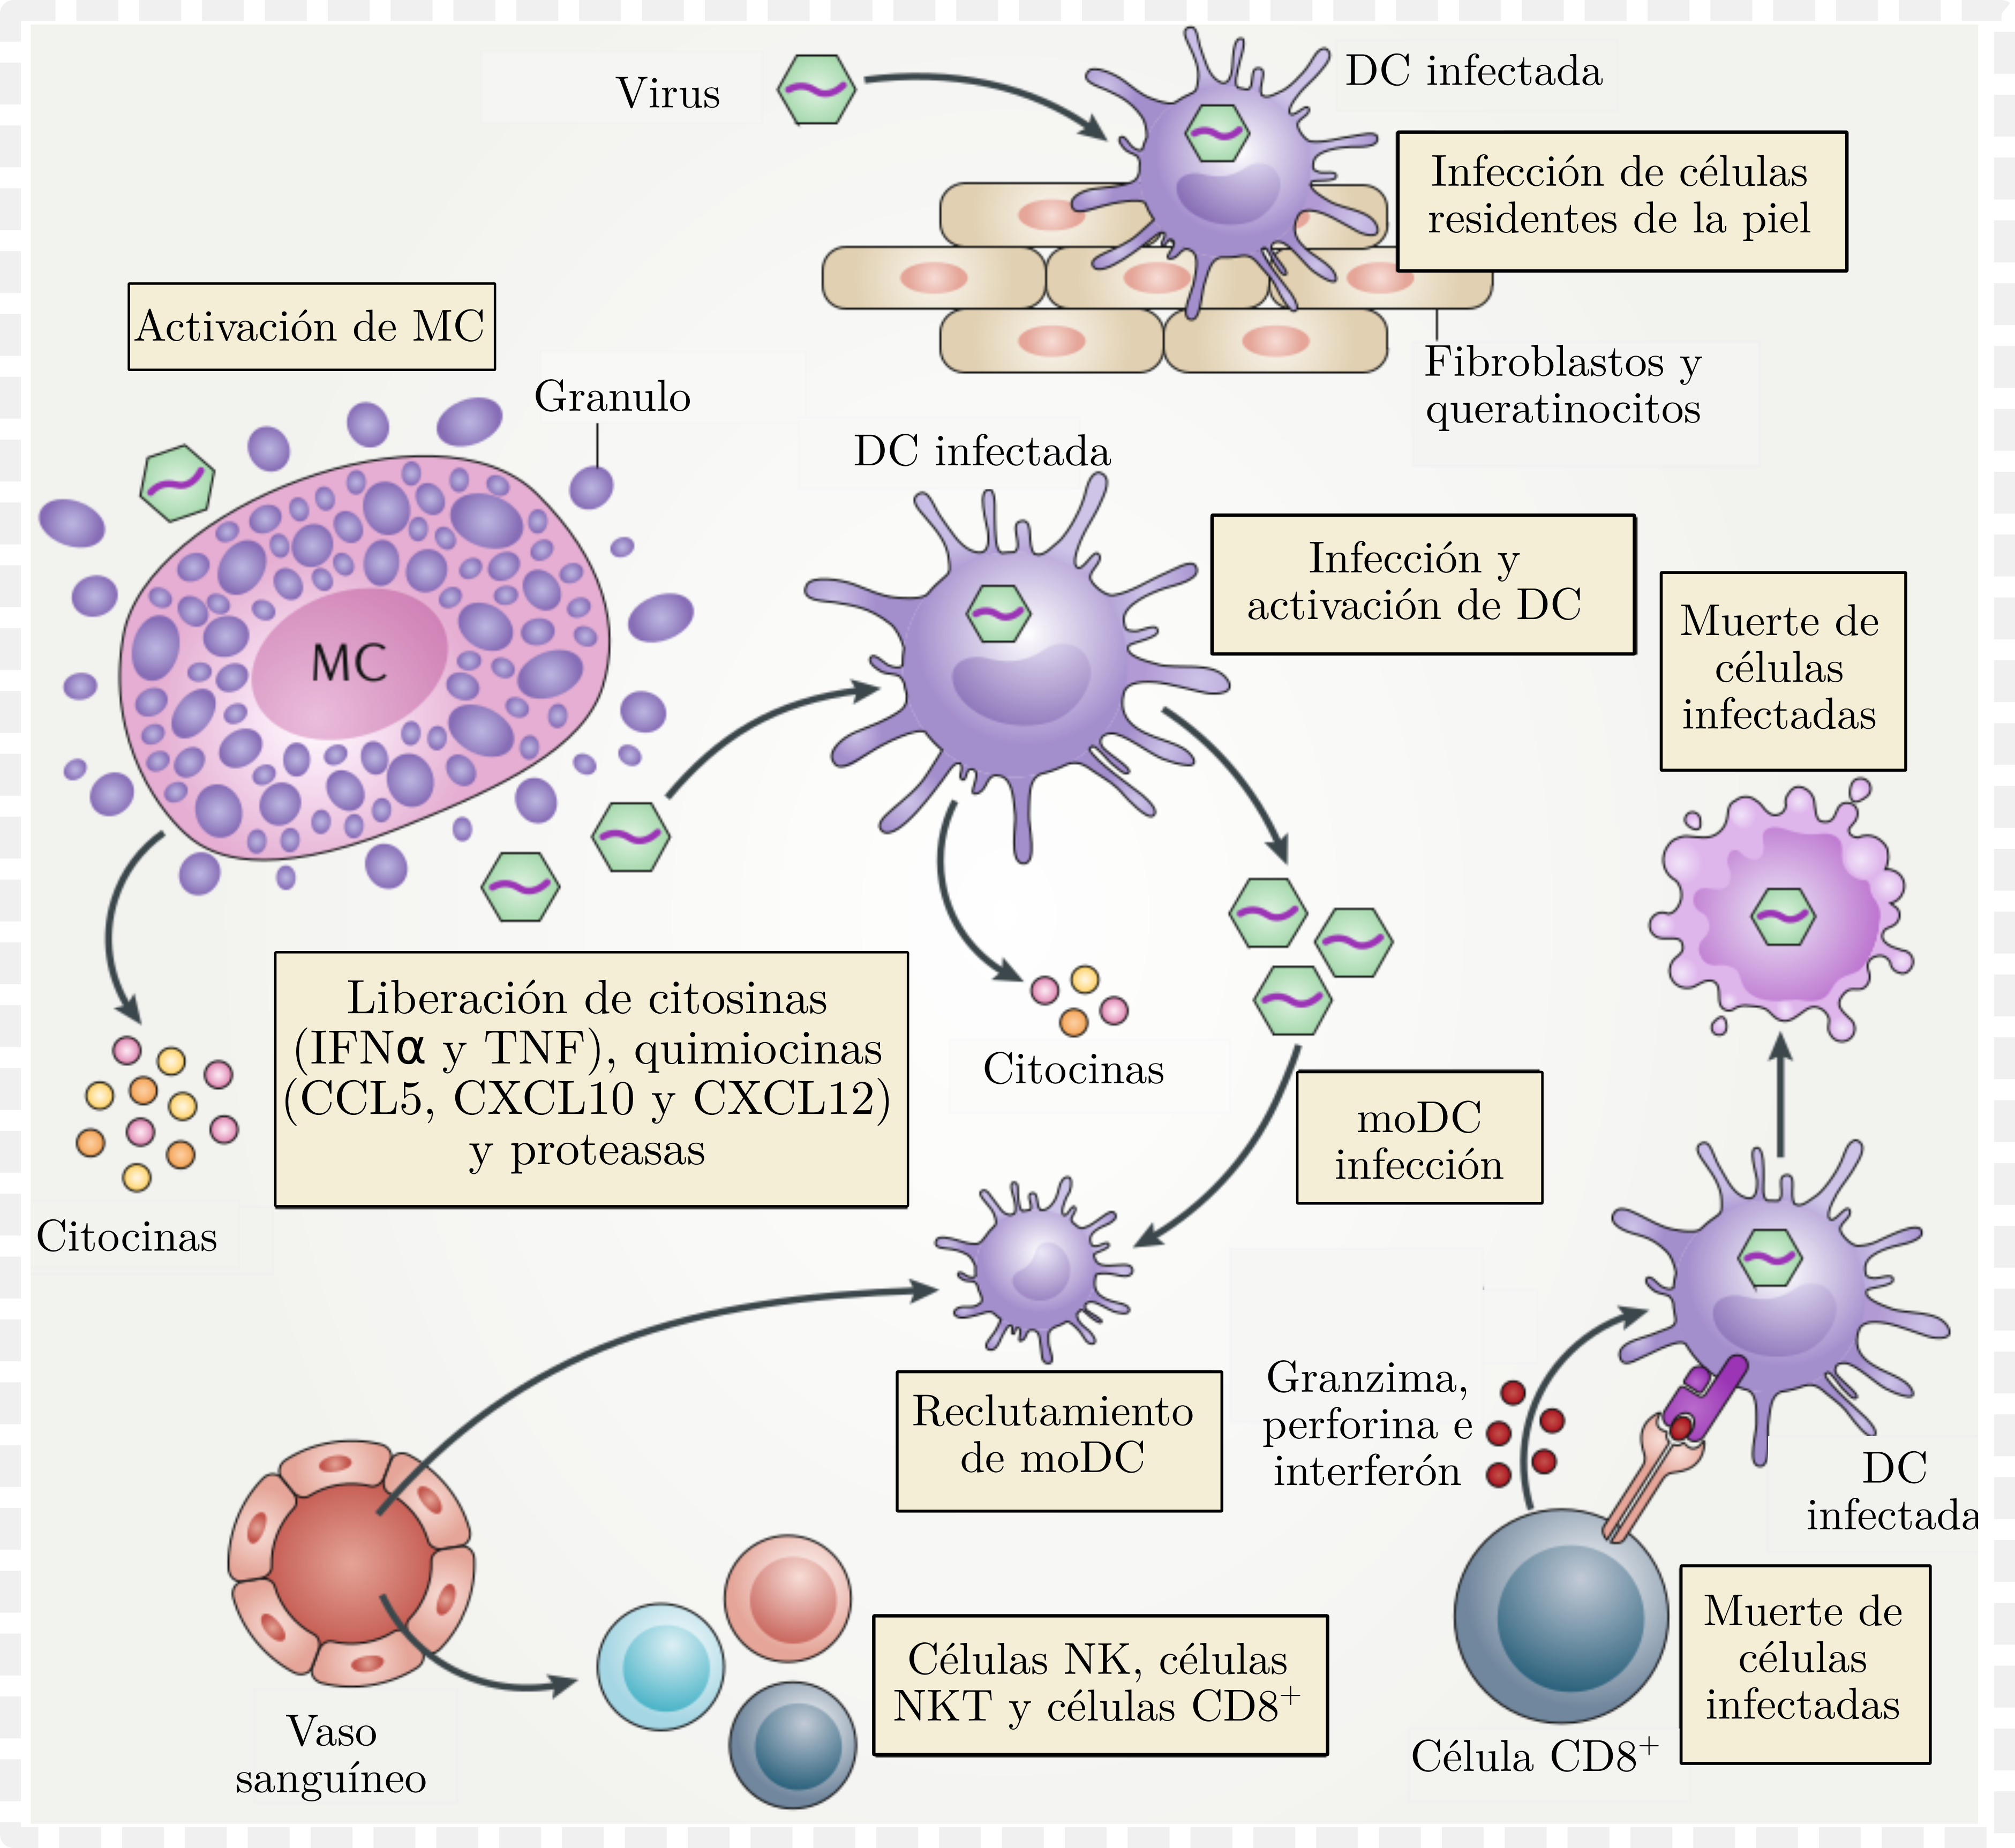
\includegraphics[width=0.7\textwidth]{imagenes/Ant/patologia.png}
  }{
    \framebox[0.75\textwidth]{\rule{0pt}{3.5cm} [Espacio reservado: Inmunopatología dérmica e interacción con células centinela]}
  }
  \caption{Fase inicial de la respuesta inmunológica local y activación de células centinela en la dermis tras la inoculación de DENV \textit{[Fuente de la imagen pendiente de identificar]}.}
  \label{Fig:patologia_piel}
\end{figure}

La inoculación del DENV ocurre cuando la hembra infectada de \textit{Aedes aegypti} deposita saliva contaminada en la piel del huésped durante la alimentación. Tras la replicación en los tejidos secundarios del vector, los viriones infecciosos se liberan en el microambiente cutáneo. Una vez en el organismo, el virus demuestra un amplio tropismo celular al interactuar con diversos receptores de superficie. Esta propiedad le permite infectar células epiteliales, fibroblastos, monocitos, macrófagos, células dendríticas, linfocitos B y T, células endoteliales y hepatocitos \cite{nanaware2021dengue}.

\section{Fisiopatología Local y Viremia Sistémica}
% Nota bibliográfica original pendiente de correspondencia: (10)
 En el sitio de inoculación dérmica, el DENV entra en contacto inmediato con las células centinela de la inmunidad innata. Entre ellas destacan las células de Langerhans (LC), las células dendríticas dérmicas (DC) y los mastocitos (MC). Los mastocitos detectan las partículas virales en cuestión de minutos y responden mediante una rápida desgranulación. Este proceso libera mediadores inflamatorios como interferón alfa (IFN-$\alpha$), factor de necrosis tumoral (TNF) y quimiocinas de atracción celular (CCL5, CXCL10 y CXCL12). A su vez, esta respuesta promueve el reclutamiento de linfocitos T citotóxicos CD8$^+$, células asesinas naturales (NK) y células NKT \textbf{(véase la Figura \ref{Fig:patologia_piel})}. No obstante, el virus infecta eficazmente a las células dendríticas y macrófagos residentes, utilizándolos como sitios primarios de replicación local. % Nota bibliográfica original pendiente de correspondencia: (10)

Las células dendríticas infectadas migran por los vasos linfáticos aferentes hacia los ganglios linfáticos regionales. En este punto, entran en contacto con nuevas poblaciones de macrófagos y monocitos a los cuales infectan. A partir de esta amplificación en el sistema linfoide, el virus se disemina por el torrente sanguíneo, originando una viremia sistémica. De esta manera, el patógeno logra colonizar órganos secundarios como el bazo, los riñones, los pulmones y el hígado. El estado virémico es detectable entre 24 y 48 horas antes del inicio de los síntomas y suele persistir de 10 a 12 días. Si un mosquito susceptible se alimenta durante este periodo, el ciclo biológico del virus se perpetúa \cite{nanaware2021dengue}.

La colonización de los ganglios linfáticos convierte a estas estructuras en centros de replicación viral masiva. Este paso resulta esencial para la consolidación de la viremia y para la subsecuente presentación de antígenos al sistema inmune adaptativo \cite{st2019adaptive}.

\section{Inmunopatología del Dengue Secundario}
 La efectividad de la respuesta inmune depende de la capacidad neutralizante de los anticuerpos dirigidos contra los dominios de la envoltura (E, prM/M) y la proteína no estructural NS1. Una infección primaria por un serotipo específico genera inmunidad permanente frente a ese mismo serotipo homotípico. Sin embargo, ante una infección secundaria por una cepa heterotípica, los anticuerpos preexistentes solo proporcionan una protección parcial y temporal. Por otro lado, la ARN polimerasa viral carece de actividad de corrección de pruebas, lo que otorga al DENV una elevada tasa de mutación y gran variabilidad antigénica. Estas variaciones permiten al virus escapar de la neutralización efectiva, desencadenando el fenómeno de Aumento Dependiente de Anticuerpos (ADE, por sus siglas en inglés).
La severidad de las manifestaciones clínicas está modulada tanto por factores virales (serotipo y mutaciones específicas) como por factores del huésped (edad y perfil inmunológico previo) \cite{dhole2024host}.

En el ámbito de la inmunidad celular, la proteína no estructural NS3 se considera el blanco inmunodominante para la respuesta de linfocitos T citotóxicos CD8$^+$ y T colaboradores CD4$^+$. Sin embargo, la baja homología de secuencia entre los cuatro serotipos (entre el 50\% y el 60\%) limita la reactividad cruzada protectora. Durante una infección secundaria heteróloga (especialmente por el serotipo 2, DENV-2), los anticuerpos no neutralizantes forman inmunocomplejos con el virus. Estos complejos facilitan la entrada viral a monocitos y macrófagos a través de los receptores Fc$\gamma$R, incrementando exponencialmente la carga viral. Como consecuencia, se desencadena una liberación masiva de mediadores inflamatorios (tormenta de citocinas) y una activación inadecuada de las células T de memoria (Pecado Antigénico Original). Este proceso culmina en complicaciones graves como la fuga vascular, la fiebre hemorrágica por dengue y el síndrome de choque \textbf{véase la Figura \ref{Fig:inmunopatogenia_tikz}} \cite{st2019adaptive}.
\begin{figure}[H]
\centering
\resizebox{\textwidth}{!}{%
\begin{tikzpicture}[
    node distance=1.2cm and 1.0cm,
    primary/.style={rectangle, draw=blu1, fill=blu, text width=3.8cm, align=center, rounded corners, minimum height=1.2cm, thick},
    secondary/.style={rectangle, draw=red!70, fill=red!5, text width=3.8cm, align=center, rounded corners, minimum height=1.2cm, thick},
    arrow/.style={-Stealth, thick, draw=gray!80}
]

    % --- COLUMNA IZQUIERDA: INFECCIÓN PRIMARIA ---
    \node (prim) [primary] {\textbf{Infección Primaria} \\ Serotipo DENV$_1$};
    \node (cent) [primary, below=of prim, yshift=-0.3cm] {Infección de Centinelas \\ (DC, Macrófagos, MC)};
    \node (gl) [primary, below=of cent, yshift=-0.3cm] {Migración a Ganglios \\ Activación CD4$^+$, CD8$^+$ y Ab};
    \node (res) [primary, below=of gl, yshift=-0.3cm, fill=green!5, draw=green!60] {\textbf{Enfermedad Autolimitada} \\ Aclaramiento viral};

    % Flechas Columna Izquierda
    \draw [arrow] (prim) -- (cent);
    \draw [arrow] (cent) -- (gl);
    \draw [arrow] (gl) -- (res);

    % --- COLUMNA DERECHA: INFECCIÓN SECUNDARIA ---
    \node (ade) [secondary, right=3.5cm of cent] {\textbf{1. Fenómeno ADE} \\ Ab previos no neutralizan $\rightarrow$ Entrada vía Fc$\gamma$R $\rightarrow$ $\uparrow$ Carga Viral};
    \node (pao) [secondary, right=1.0cm of ade] {\textbf{2. Pecado Antigénico} \\ T-memoria ineficaces $\rightarrow$ Tormenta de Citocinas};
    \node (sec) [secondary, above=1.2cm of ade, xshift=2.5cm] {\textbf{Infección Secundaria} \\ Serotipo Heterólogo (DENV$_2$)};
    \node (shock) [secondary, below=1.5cm of ade, xshift=2.5cm, fill=red!20, draw=red!90, text width=5.2cm] {\textbf{Enfermedad Grave} \\ Fuga Vascular y Síndrome de Choque};

    % Flechas Columna Derecha
    \draw [arrow] (sec) -- (ade);
    \draw [arrow] (sec) -- (pao);
    \draw [arrow] (ade) -- (shock);
    \draw [arrow] (pao) -- (shock);

\end{tikzpicture}
}
\caption{Inmunopatogenia comparativa del dengue: evolución clínica diferencial entre la infección primaria autolimitada y la infección secundaria grave.}
\label{Fig:inmunopatogenia_tikz}
\end{figure}

\section{Ciclo de Replicación Intracelular y Maduración Viral}
El ciclo de replicación celular del virus del dengue (DENV) constituye un proceso molecular dinámico y altamente coordinado que involucra la reorganización de los compartimentos membranosos del huésped, desde la internalización endocítica hasta la maduración proteolítica en la vía secretora \cite{uno2023dengue,stjohn2023dengue}. Durante esta cascada, la interacción de las proteínas virales con la maquinaria celular permite la síntesis del genoma y el ensamblaje de nuevas partículas infectivas \textbf{véase la Figura \ref{Fig:ciclo_replicacion}}. Las etapas fundamentales que componen este ciclo intracelular se describen a continuación:

\begin{figure}[H]
  \centering
  \IfFileExists{imagenes/Ant/ciclo.png}{
    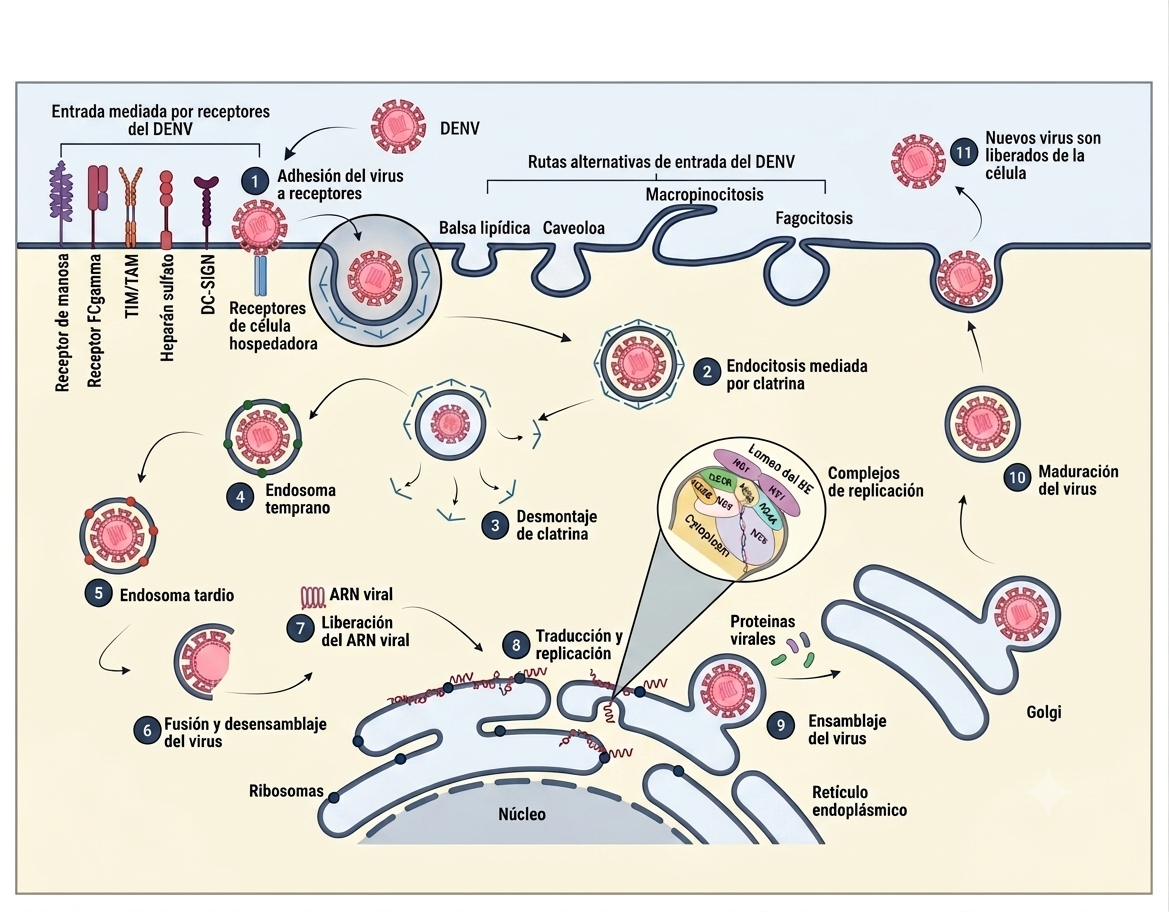
\includegraphics[width=0.85\textwidth]{imagenes/Ant/ciclo.png}
  }{
    \framebox[0.85\textwidth]{\rule{0pt}{5cm} [Espacio reservado: Esquema del ciclo de replicación celular del DENV]}
  }
  \caption{Representación esquemática del ciclo de replicación intracelular del virus del dengue (DENV).}
  \label{Fig:ciclo_replicacion}
\end{figure}

\begin{enumerate}
    \item \textbf{Adhesión celular e internalización:} La partícula viral se une a receptores de membrana específicos en la superficie de la célula hospedera, iniciando la internalización mediante endocitosis mediada por clatrina.
    \item \textbf{Formación de la vesícula endocítica:} El virión es reclutado en fosas revestidas de clatrina para constituir la vesícula de transporte interiorizada.
    \item \textbf{Desnudamiento del revestimiento:} Se produce la liberación de la cubierta de clatrina, dando paso a la maduración de la vesícula hacia un endosoma temprano.
    \item \textbf{Tránsito endosómico temprano:} El endosoma temprano, caracterizado por la presencia de la GTPasa Rab5, mantiene un pH aproximado de 6.5.
    \item \textbf{Acidificación endosómica tardía:} El endosoma madura a endosoma tardío (marcado por la proteína Rab7), donde la bomba de protones reduce el pH interno a valores cercanos a 5.5.
    \item \textbf{Fusión de membranas:} El entorno ácido induce cambios conformacionales en la glucoproteína E de la envoltura viral, desencadenando la fusión entre la membrana viral y la membrana endosómica.
    \item \textbf{Desensamblaje y liberación del genoma:} Se libera la nucleocápside al citosol celular, permitiendo la desagregación del genoma de ARN monocatenario de polaridad positiva (+ssRNA).
    \item \textbf{Traducción y replicación en el Retículo Endoplásmico (RE):} El ARN viral es traducido en el RE para sintetizar una poliproteína única que es procesada por proteasas virales ($\text{NS2B-NS3}$) y celulares. Las invaginaciones en la membrana del RE conforman los complejos de replicación.
    \item \textbf{Ensamblaje inmaduro:} El genoma replicado y las proteínas estructurales se ensamblan en la superficie del RE, brotando hacia el lumen celular como partículas virales inmaduras e inefectivas.
    \item \textbf{Maduración por Furina:} Los viriones inmaduros se transportan a través de la Red Trans-Golgi (TGN), donde la proteasa hospedera furina escinde la proteína prM, generando partículas virales maduras y potencialmente infectivas.
    \item \textbf{Exocitosis:} Los viriones maduros son liberados al espacio extracelular mediante vesículas secretoras, completando el ciclo de infección e iniciando la propagación sistémica \cite{screaton2015new}
\end{enumerate}

\section{Estrategias de Inhibición de la Proteasa NS2B-NS3 en DENV-2}
Existen determinadas familias químicas de inhibidores de la proteasa \textbf{NS2B-NS3 de DENV-2}, debido a que la proteasa heterodimérica NS2B-NS3 de DENV-2 es un blanco terapéutico esencial para el desarrollo de antivirales. Para su procesamiento proteolítico, la enzima fluctúa entre dos conformaciones principales: una \textbf{conformación abierta (inactiva)}, donde la región C-terminal del cofactor NS2B está desordenada o libre, y una \textbf{conformación cerrada (activa)}, en la que NS2B envuelve al dominio proteasa NS3 formando un cinturón $\beta$ que completa el sitio activo \cite{chandramouli2010serotype, maus2021sar}.

A partir de esta dinámica estructural, se han desarrollado diversas familias de inhibidores que actúan mediante distintos mecanismos de acción:

\vspace{0.5em}

\subsection{Estrategias de Inhibición de la Proteasa NS2B-NS3 en DENV-2}
Esta clase de compuestos no competitivos posee un núcleo central de quinoxalina. En la posición 2 presenta una fracción de amina cíclica (como prolina, pirrolidina o piperidina), mientras que las posiciones 3 y 7 contienen diversos sustituyentes lipofílicos.

\begin{itemize}
    \item \textbf{Mecanismo de acción:} Se unen a un bolsillo alostérico situado en el lado opuesto de la tríada catalítica. Esta interacción bloquea la transición de la enzima hacia su forma activa (cerrada). De esta manera, se impide que el cofactor NS2B se asocie correctamente con el dominio NS3 \cite{zephyr2023allosteric}.
    \item \textbf{Residuos de interacción en DENV-2:} La cavidad alostérica está definida por los residuos \textbf{Gln74, Trp83, Ile123, Asn152 y Val155} en NS3. Al respecto, experimentos con ``trampas de disulfuro'' (entre \textbf{Lys117} en NS3 y \textbf{Ser75} en NS2B) confirmaron que estos inhibidores pierden eficacia cuando la proteína queda atrapada en su forma cerrada. Este hallazgo demuestra la superposición entre su sitio de acción y la interfaz de unión de NS2B.
    \item \textbf{Compuestos destacados y potencia:}
    \begin{itemize}
        \item \textbf{Compuesto 32} (análogo de piperidina con grupo guanidinio): $\text{IC}_{50} = 130 \pm 9\ \mu\text{M}$ (enzimático); $\text{EC}_{50} = 2.7\ \mu\text{M}$ (celular, el más potente en ensayos celulares contra DENV-2).
        \item \textbf{Compuesto 19} (análogo de pirrolidina): $\text{IC}_{50} = 160 \pm 8\ \mu\text{M}$.
        \item \textbf{Compuestos 33 y 36}: Derivados con notable potencia antiviral celular ($\text{EC}_{50} = 4.6\ \mu\text{M}$ y $4.4\ \mu\text{M}$, respectivamente) \cite{zephyr2023allosteric}.
    \end{itemize}
\end{itemize}
\subsection{Inhibidores Alostéricos (Benzotiazol y Benzofurano)}

Esta serie de compuestos no competitivos fue diseñada para unirse al bolsillo alostérico adyacente al residuo \textbf{Asn152}. Este aminoácido actúa como un \textbf{``interruptor molecular''} ubicado entre la cavidad activa y la alostérica. De este modo, regula la transición entre la conformación abierta e inactiva de la enzima.

\begin{itemize}
    \item \textbf{Mecanismo de acción:} Estabilizan la proteasa en su conformación abierta e inactiva mediante inhibición no competitiva. Al respecto, estudios de mutagénesis con cisteína única (mutante T122C y bloqueo con N-bencilmaleimida) confirmaron que estos inhibidores se ubican cerca del residuo \textbf{Thr122} y del bucle de los residuos 120s.
    \item \textbf{Residuos de interacción en DENV-2:} El farmacóforo clave (motivo catecol 5,6-dihidroxi) forma una red conservada de puentes de hidrógeno con \textbf{Lys74, Gly148 y Asn152}. Asimismo, interacciona con residuos del bolsillo lipofílico como \textbf{Met49, Leu76, Trp83, Lys84, Leu85, Glu86, Glu88, Trp89, Val146, Val147, Leu149, Ala164, Ile165 e Ile166}.
    \item \textbf{Compuestos destacados y potencia:}
    \begin{itemize}
        \item \textbf{Compuesto 34e (Derivado de Benzofurano):} Reemplaza el núcleo de benzotiazol mediante \textit{scaffold hopping}. La geometría ligeramente inclinada del benzofurano favorece la interacción entre el carbonilo de la amida y la \textbf{Lys74} de DENV-2. Esto le permite alcanzar una elevada potencia enzimática con un valor de $\text{IC}_{50} = 0.69 \pm 0.16\ \mu\text{M}$ ($0.73 \pm 0.015\ \mu\text{M}$ en el mutante T120A/N167Q).
        \item \textbf{Compuesto 25b (Benzotiazol truncado con yodo en \textit{para}):} Diseñado para maximizar la eficiencia de ligando ($\text{LE} = 0.41$). Presenta una $\text{IC}_{50} = 4.38 \pm 0.38\ \mu\text{M}$ ($K_i = 7.67\ \mu\text{M}$) contra DENV-2 y una marcada actividad en replicones virales celulares. En este caso, el átomo de yodo orientado hacia \textbf{Glu86/Glu88} favorece una interacción carboxilato-halógeno altamente efectiva.
        \item \textbf{Compuesto 23b (Estructura en forma de ``Y'', derivado del ácido 2,2-difenilacético):} Muestra una $\text{IC}_{50} = 11.12 \pm 0.49\ \mu\text{M}$ contra DENV-2. Fue diseñado para abarcar de forma simultánea las dos subcavidades hidrofóbicas que ocupan los enantiómeros de prolina. Su prodroga dimetoxilada (\textbf{22b}) logró reducir significativamente la replicación celular del ARN de DENV-2 gracias a una mayor permeabilidad de membrana \cite{maus2021sar}.
    \end{itemize}
\end{itemize}

\subsection{Inhibidores Ortostéricos y Modulación Mecánica (Rigidificación)}

\begin{itemize}
    \item \textbf{Inhibidores Competitivos Ortostéricos:} Se dirigen directamente a la cavidad del sitio activo unida a la tríada catalítica (\textbf{His51, Asp75, Ser135}).
    \begin{itemize}
        \item \textit{Limitación principal:} El sitio activo de la proteasa flaviviral es muy superficial y cargado negativamente, mostrando preferencia por residuos dibásicos en las posiciones $P1$ y $P2$. Los miméticos del sustrato suelen presentar propiedades farmacocinéticas deficientes y una pobre permeabilidad a través de las membranas celulares.
    \end{itemize}
    \item \textbf{Estrategia de Rigidificación (Efecto Alostérico Mecánico):} Propuesta a partir de la identificación del tramo de 10 residuos en NS3 (residuos 11 al 20). Dado que la proteasa requiere flexibilidad estructural para llevar a cabo la catálisis, los ligandos que reducen o rigidizan la movilidad de la enzima disminuyen drásticamente su eficiencia catalítica ($V_{\max}$) sin alterar necesariamente la capacidad de unión al sustrato ($K_m$)\cite{chandramouli2010serotype}.
\end{itemize} \newpage

 \subsection{Tabla Comparativa de Inhibidores de la Proteasa NS2B-NS3}
 \begingroup
\scriptsize % Tamaño de letra adaptado para 6 columnas
\setlength{\tabcolsep}{1.5pt} % Espaciado lateral de seguridad entre columnas
\begin{xltabular}{\textwidth}{
  >{\hsize=0.9\hsize\RaggedRight\arraybackslash}X
  >{\hsize=0.7\hsize\RaggedRight\arraybackslash}X
  >{\hsize=1.1\hsize\RaggedRight\arraybackslash}X
  >{\hsize=1.1\hsize\RaggedRight\arraybackslash}X
  >{\hsize=1.1\hsize\RaggedRight\arraybackslash}X
  >{\hsize=1.1\hsize\RaggedRight\arraybackslash}X
}
\caption{Resumen de inhibidores y sitios de unión.} \label{tab:inhibidores} \\ % <--- AQUÍ VA EL CAPTION
\toprule
\textbf{Familia /\allowbreak Compuesto} & \textbf{Sitio de Unión} & \textbf{Regiones y Residuos Clave (DENV-2)} & \textbf{Eficacia /\allowbreak Potencia Reportada} & \textbf{Importancia Estratégica} & \textbf{Limitaciones Principales} \\
\midrule
\endhead

\bottomrule
\endfoot

\textbf{Quinoxalinas} \newline (\textit{Comp. 32, 19, 33, 36}) & \textbf{Alostérico} \newline (Interfaz distal) & \textbf{NS3:} Q74, W83, I123, N152, V155 \newline \textbf{Evidencia:} K117 (NS3) y S75 (NS2B) [trampa disulfuro] & \textbf{Comp. 32:} \newline $\text{IC}_{50} = 130 \pm 9\ \mu\text{M}$ \newline $\text{EC}_{50} = 2.7\ \mu\text{M}$ \newline \textbf{Comp. 19:} \newline $\text{IC}_{50} = 160 \pm 8\ \mu\text{M}$ & Desplaza al cofactor NS2B e impide que la proteasa pase de la forma abierta a la cerrada activa. & Pobre correlación entre baja potencia enzimática in vitro y alta eficacia en ensayos celulares. Escasez de estructuras cristalinas en complejo. \\
\midrule
\textbf{Benzofurano 34e} & \textbf{Alostérico} \newline (Cercano a N152)& \textbf{NS3:} K74 (interacción mejorada con carbonilo), G148, N152 (motivo catecol)& $\text{IC}_{50} = 0.69 \pm 0.16\ \mu\text{M}$ \newline ($0.73 \pm 0.015\ \mu\text{M}$ en mutante T120A/\allowbreak N167Q) & Reemplazo por benzofurano adapta mejor la geometría a Lys74 de DENV-2, eliminando preferencia por ZIKV. & Reducida eficacia en replicación celular de DENV-2 atribuida a permeabilidad o metabolismo celular \cite{maus2021sar}. \\
\midrule
\textbf{Benzotiazol Truncado 25b} \newline (\textit{p-yodobenzamida}) & \textbf{Alostérico} \newline (Entrada al bolsillo alostérico) & \textbf{NS3:} K74, G148, N152 \newline \textbf{Residuos ácidos:} E86, E88 (contacto con yodo) & $\text{IC}_{50} = 4.38 \pm 0.38\ \mu\text{M}$ \newline $K_i = 7.67\ \mu\text{M}$\newline Disminución significativa de replicación de ARN celular & Excelente eficiencia de ligando ($\text{LE} = 0.41$). Interacción halógeno-carboxilato con Glu86/88 incrementa afinidad. & Requiere grupo dihidroxi (catecol) libre para actividad enzimática directa, sensible a oxidación in vitro \cite{maus2021sar}. \\
\midrule
\textbf{Inhibidores en ``Y''} \newline (\textit{Compuesto 23b}) & \textbf{Alostérico} \newline (Subbolsillos hidrofóbicos) & \textbf{NS3:} Subcavidades definidas por W89, A166, V146, V147 y N152 & $\text{IC}_{50} = 11.12 \pm 0.49\ \mu\text{M}$ \newline \textbf{Prodroga 22b:} Inhibición marcadamente potente en replicones & Ocupa simultáneamente las dos subcavidades lipofílicas exploradas por enantiómeros de prolina. & Restricción geométrica de la estructura en Y puede distorsionar la alineación del motivo catecol \cite{maus2021sar}. \\
\midrule
\textbf{Análogos de Sustrato} & \textbf{Ortostérico} \newline (Sitio activo) & \textbf{NS3:} Tríada catalítica (H51, D75, S135) y bolsillos $P1/\allowbreak P2$ & Variable (alta afinidad in vitro en péptidos optimizados)& Bloqueo directo del centro catalítico primario, región conservada entre serotipos. & Farmacocinética muy deficiente y mala permeabilidad debido a cargas dibásicas en P1/\allowbreak P2 \cite{cavina2024orthoflaviviral}. \\
\midrule
\textbf{Rigidificación} & \textbf{Alostérico /\allowbreak Mecánico} & \textbf{NS3:} Tramo regulador de 10 aminoácidos (residuos 11 al 20 en NS3pro) & Modulación de la constante catalítica ($V_{\max}$) sin alterar $K_m$ & Elimina la flexibilidad estructural necesaria para la catálisis; estrategia de amplio espectro. & Requiere diseñar moléculas pequeñas que restrinjan la dinámica sin depender del sitio activo \cite{chandramouli2010serotype}. \\
\end{xltabular}
\endgroup

\section{Manifestaciones Clínicas}
La infección por el virus del dengue presenta un periodo de incubación de 3 a 10 días y evoluciona en tres fases clínicas secuenciales. La \textbf{fase febril} (2 a 7 días) inicia de forma súbita con fiebre alta, frecuentemente bifásica. Esta etapa se acompaña de cefalea, dolor retroorbitario, mialgias, artralgias, exantema cutáneo y síntomas gastrointestinales. A continuación acontece la \textbf{fase crítica} (3 a 5 días), la cual coincide con la defervescencia. Esta fase se caracteriza por un aumento en la permeabilidad vascular, fuga plasmática, hemoconcentración y trombocitopenia, lo que conlleva un elevado riesgo de hemorragias y choque. Finalmente, la \textbf{fase de recuperación} (2 a 3 días) se distingue por la reabsorción del líquido extravascular, la estabilización hemodinámica y el retorno del apetito \cite{contreras2021aspectos, roquefactores}.

El desarrollo de formas graves de la enfermedad (dengue grave y síndrome de choque por dengue) depende de una interacción compleja entre factores del huésped, del virus y epidemiológicos. Entre los factores del huésped destacan la edad, el estado nutricional y el perfil genético; por su parte, los factores virales incluyen el serotipo y la virulencia de la cepa. En particular, una infección secundaria heterotípica incrementa de manera exponencial el riesgo de severidad mediante el mecanismo de amplificación dependiente de anticuerpos (ADE). En este proceso, los anticuerpos preexistentes facilitan la entrada viral a los macrófagos y desencadenan una liberación masiva de citocinas. Aunque este fenómeno ocurre principalmente en infecciones secundarias, también se han documentado cuadros graves durante primoinfecciones, asociados sobre todo a los serotipos DENV-2 y DENV-3 \textbf{véase la Figura \ref{fig:sintomas_dengue}} \cite{fajardo2012dengue}.

\begin{figure}[H]
    \centering
    \begin{tikzpicture}[
        node distance=1.5cm,
        block/.style={rectangle, draw=black, thick, rounded corners, text width=5.2cm, align=left, minimum height=2cm, font=\small},
        title/.style={font=\bfseries\small, align=center, minimum height=0.6cm}
    ]

    % --- BLOQUE INICIAL (DENGUE NO GRAVE) ---
    \node[block, fill=azuli] (nograve) {
        \textbf{DENGUE NO GRAVE}\\
        \textit{(Clásico / Fiebre por dengue)}\\[0.2cm]
        • Fiebre súbita y cefalea frontal.\\
        • Mialgias, artralgias y fotofobia.\\
        • Dolor retroorbitario.\\
        • Exantema rubeoliforme.\\
        • Manifestaciones mucocutáneas leves por vasodilatación.
    };

    % --- BLOQUE DENGUE GRAVE ---
    \node[block, fill=azuld, right=0.8cm of nograve] (grave) {
        \textbf{DENGUE GRAVE}\\
        \textit{(Fiebre hemorrágica)}\\[0.2cm]
        • \textbf{Fuga capilar:} Ascitis, derrame pleural/pericárdico, edema.\\
        • Trombocitopenia ($<100,000\text{ mm}^3$).\\
        • Hemorragias activas o ocultas (digestivas, pulmonares, etc.).\\
        • Prueba de torniquete (+).
    };

    % --- BLOQUE SÍNDROME DE CHOQUE ---
    \node[block, fill=rojocho, below=1.2cm of grave] (choque) {
        \textbf{SÍNDROME DE CHOQUE}\\[0.2cm]
        • \textbf{Falla circulatoria:} TA diferencial $<20\text{ mmHg}$ o sistólica $<60\text{ mmHg}$.\\
        • \textbf{Signos de choque:} Alteración de conciencia, piel fría, diaforesis, pulso débil y oliguria.\\
        • \textbf{Predictores:} Hematocrito $>50\%$ y plaquetas $\le 75,000$.
    };

    % --- TÍTULO SUPERIOR ---
    \node[title, text width=11.5cm, draw, fill=gray!20, above=0.8cm of $(nograve.north)!0.5!(grave.north)$] (titulo) {
        MANIFESTACIONES CLÍNICAS Y EVOLUCIÓN DEL DENGUE
    };

    % --- FLECHAS CONECTORAS ---
    \draw[-{Stealth}, thick] (titulo.south) -- ++(0,-0.3) -| (nograve.north);
    \draw[-{Stealth}, thick] (titulo.south) -- ++(0,-0.3) -| (grave.north);
    
    \draw[-{Stealth}, thick, dashed] (grave.south) -- (choque.north) 
        node[pos=0.5, right, font=\tiny\itshape, text width=2.5cm] {Respuesta inflamatoria e inmunológica};

    \end{tikzpicture}
    \caption{Esquema de las manifestaciones clínicas del dengue según su severidad.}
    \label{fig:sintomas_dengue}
\end{figure}

Para la confirmación diagnóstica del dengue se requiere la determinación de anticuerpos IgM o IgG, la detección del antígeno NS1 en suero o el aislamiento viral. La prueba de laboratorio más utilizada es la determinación de IgM por ELISA, al ser el primer marcador de respuesta inmunitaria en aparecer hacia el quinto día del cuadro agudo (detectable en el 80\% de los pacientes y con una persistencia de hasta tres meses) \cite{fajardo2012dengue}. 

\subsection{Tratamiento y Desafíos Terapéuticos en la Infección por DENV}

En el contexto de la inmunopatogénesis del dengue, la infección por un serotipo otorga una respuesta inmunológica protectora de por vida contra ese mismo tipo. Sin embargo, la inmunidad cruzada o heterotípica contra los demás serotipos es únicamente de corta duración. Tras disminuir esta protección temporal, una infección secundaria heteróloga incrementa el riesgo de desarrollar formas graves de la enfermedad mediante el mecanismo de amplificación dependiente de anticuerpos (ADE). Asimismo, en regiones hiperendémicas donde coexisten varios serotipos, se han registrado coinfecciones virales complejas. Este fenómeno resulta crítico en el desarrollo de biológicos, pues se ha observado un aumento en la gravedad del cuadro clínico en personas seronegativas tras ser vacunadas debido al proceso de ADE. Por ello, surge la necesidad de diseñar vacunas tetravalentes que generen una respuesta inmune balanceada \cite{aynekulu2024role}.

A esta complejidad inmunológica se suma la elevada variabilidad genética del DENV, presente incluso entre cepas de un mismo serotipo. Esta condición dificulta el desarrollo de esquemas antivirales de amplio espectro. En términos generales, los avances en vacunas, fármacos e inmunoterapias se ven frenados por la interacción entre la dinámica del vector, la biología viral, la respuesta del huésped y los mecanismos fisiopatológicos subyacentes \cite{cavina2024orthoflaviviral}.

Como reflejo de estos desafíos, aunque existen vacunas autorizadas contra el DENV, su uso se limita estrictamente a personas seropositivas. Esto se debe a que la inmunización en individuos seronegativos aumenta el riesgo de sufrir cuadros graves en exposiciones posteriores por causa del ADE. Por consiguiente, hasta la fecha no se dispone de una terapia antiviral directa aprobada contra el DENV ni contra otros flavivirus como el virus del Zika (ZIKV). De este modo, el manejo clínico se restringe al tratamiento de soporte hemodinámico y sintomático. Esta falta de tratamientos evidencia la necesidad urgente de desarrollar fármacos dirigidos a blancos virales específicos \cite{maus2021sar}.

\section{Fundamentos y Propiedades de la Nanotecnología}

La nanotecnología se concibe como la investigación científica y el desarrollo tecnológico orientados a comprender y manipular la materia a nivel atómico y molecular en la nanoescala. Esta disciplina permite diseñar y fabricar estructuras, materiales, dispositivos y sistemas de complejidad creciente. Estos desarrollos destacan por presentar propiedades específicas y funciones novedosas, derivadas directamente del tamaño reducido de sus componentes \cite{domingo2010nanotecnologia}.

Respecto a su delimitación física, el límite superior del nanomundo se establece formalmente en aproximadamente $100\text{ nm}$. Esta magnitud es cientos de veces menor que la partícula más diminuta visible a simple vista e inferior al límite de resolución de los microscopios ópticos convencionales. Sin embargo, un fragmento de materia comprendido en este rango (o ligeramente superior) aún conserva el comportamiento del material masivo original. En otras palabras, se comporta esencialmente como una porción diminuta de materia ordinaria.

Para contextualizar esta escala en el ámbito biológico, entidades como los virus poseen dimensiones contenidas dentro del rango nanométrico. En cambio, microorganismos como las bacterias pertenecen a una escala sustancialmente mayor, superando de manera habitual los $10\ \mu\text{m}$ \textbf{(véase la figura: Dimensiones típicas de nanopartículas y comparación de escalas)}. Por otro lado, al examinar partículas metálicas compuestas por aproximadamente 1000 átomos, utilizadas con frecuencia en la síntesis de materiales avanzados, sus propiedades fisicoquímicas divergen significativamente de las del material macroscópico equivalente. Por consiguiente, el ensamblaje controlado de estas nanoestructuras para conformar sistemas mayores permite obtener materiales con comportamientos y funcionalidades totalmente novedosos.
\section{Nanopartículas Funcionalizadas e Interacción con Sistemas Biológicos}

Las nanopartículas funcionalizadas constituyen un ejemplo representativo del potencial de estos materiales. Un caso concreto son las nanopartículas magnéticas con estructura de tipo núcleo-coraza (\textit{core-shell}). Estas estructuras se encuentran recubiertas por una capa externa de oro que facilita la conjugación covalente de biomoléculas (como proteínas o anticuerpos) e incluso agentes farmacéuticos. En este esquema, el núcleo magnético permite guiar el complejo molecular hacia regiones anatómicas específicas mediante la aplicación de campos magnéticos externos. De este modo, se logra una administración dirigida de fármacos (\textit{targeted drug delivery}). Por otro lado, la molécula biológica acoplada puede actuar como un ligando de reconocimiento específico para células blanco (por ejemplo, células tumorales). Posteriormente, estas células pueden destruirse mediante hipertermia al aplicar un campo magnético de radiofrecuencia de baja intensidad, el cual resulta inocuo para los tejidos sanos circundantes. 

En cuanto a la interacción directa entre las nanoestructuras y los sistemas vivos, la dimensión física representa un factor crítico para la captación celular. Al respecto, estudios realizados con nanopartículas de plata en un amplio rango de tamaños demostraron que únicamente aquellas con diámetros de entre $1\text{ nm}$ y $10\text{ nm}$ logran internalizarse en las células y alterar su fisiología. Estas partículas se adhieren inicialmente a la membrana plasmática y modifican su función a través de dos mecanismos principales: por una parte, alterando la permeabilidad de la membrana y, por otra, atravesando la barrera celular para inducir daños intracelulares adicionales, entre los que destaca su posible interacción con el ADN celular. 
\subsection{Nanoestructuras de carbono}
El carbono es un elemento ligero y estructuralmente fundamental. Sus átomos contienen seis electrones: dos se ubican en la capa interna (orbital 1s), mientras que los cuatro restantes pertenecen a la capa de valencia (2s y 2p) y están disponibles para formar enlaces químicos. La gran versatilidad de estas interacciones confiere al carbono una amplia diversidad de estructuras físicas y moleculares \textbf{véase la Figura \ref{fig:alotropos-carbono}}. Por su parte, las condiciones termodinámicas durante la síntesis o cristalización —como la presión y la temperatura— determinan de manera crítica el tipo de hibridación y los enlaces que se forman \cite{martinez2024emergence}.

Como consecuencia de esta flexibilidad estructural, el carbono presenta diversas formas alotrópicas clasificadas según su dimensionalidad, entre las cuales destacan las siguientes:

\begin{figure}[H]
  \centering
  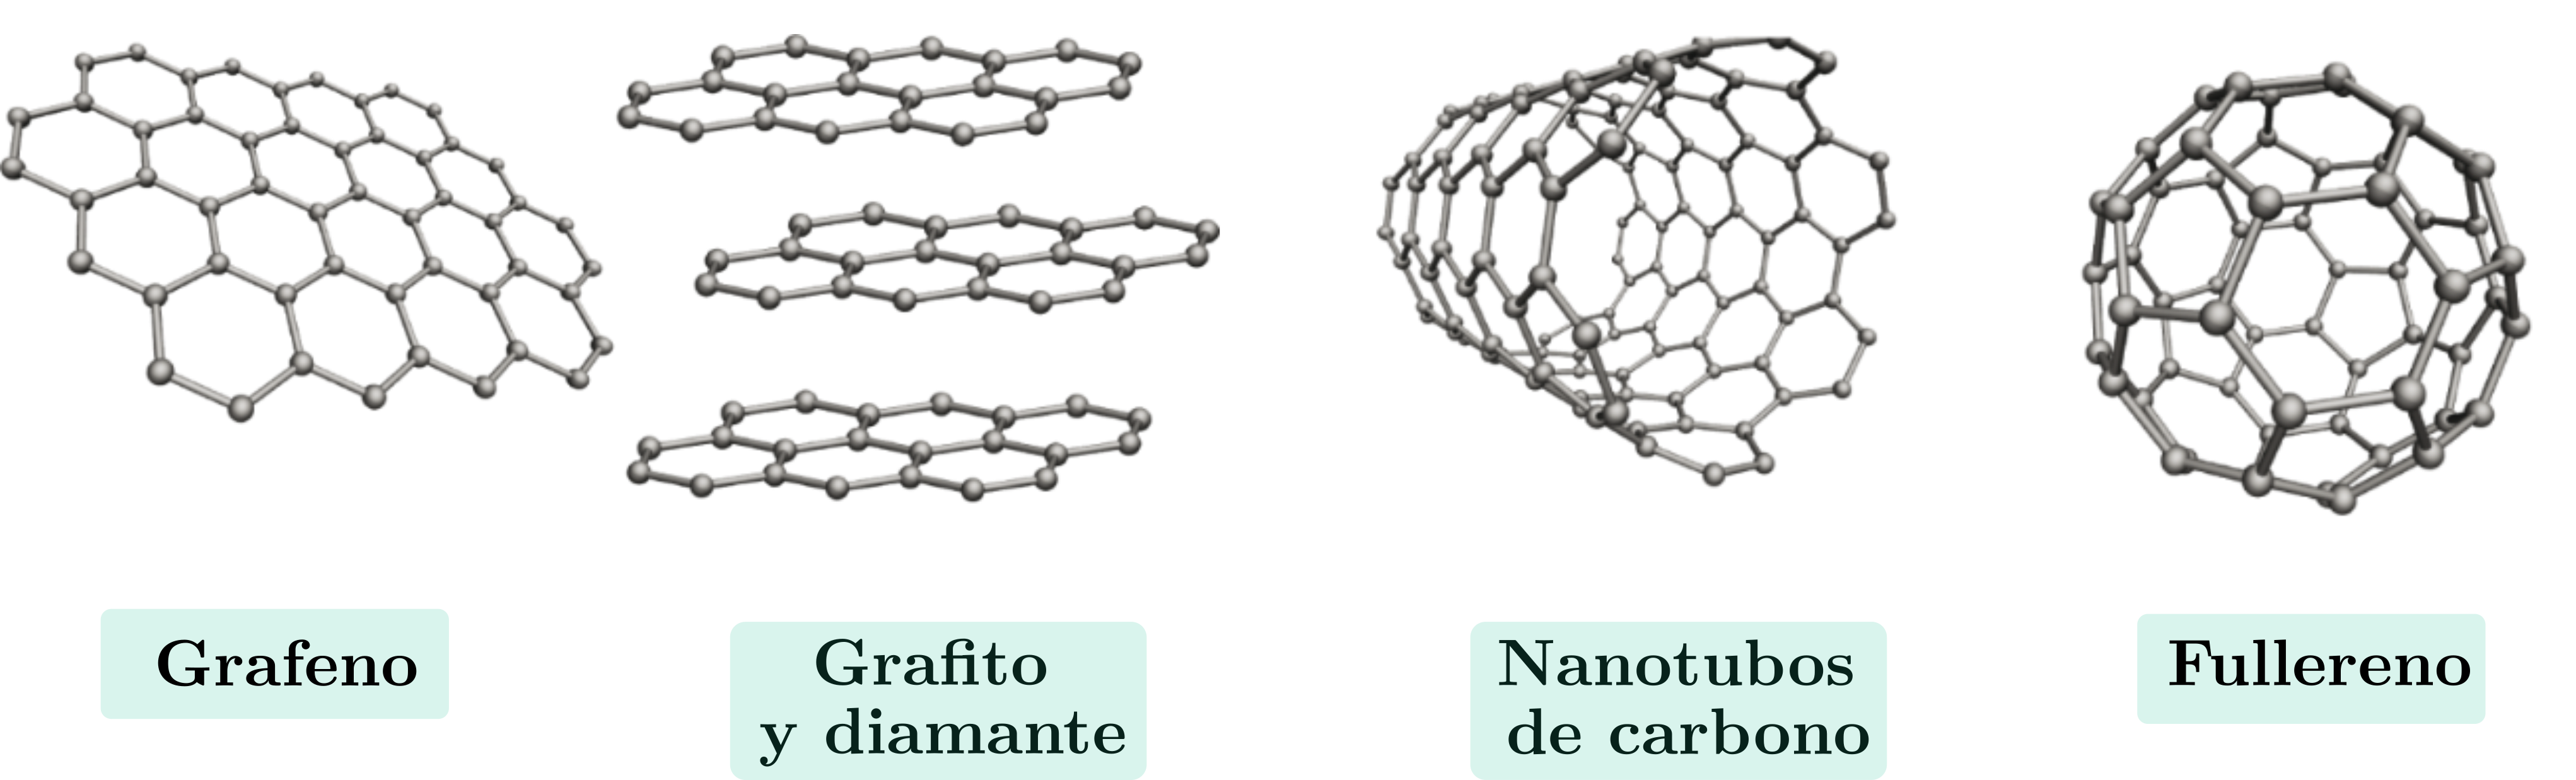
\includegraphics[width=\textwidth]{imagenes/Ant/alotropos.png}
  \caption{Representación esquemática de las principales formas alotrópicas del carbono} \cite{medrano2012grafeno}.
  \label{fig:alotropos-carbono}
\end{figure}

\subsection{Historia y Descubrimiento}
El descubrimiento del primer fulereno ocurrió en septiembre de 1985 en la Universidad Rice. Fue el resultado de una colaboración entre Harold Kroto (de la Universidad de Sussex), Robert Curl y Richard Smalley, quienes recibieron el Premio Nobel de Química en 1996 por este hallazgo. Inicialmente, el interés de Kroto se centraba en el análisis espectral de cadenas de carbono en el medio interestelar y su síntesis en el laboratorio. Para recrear estas condiciones, empleó un equipo de ablación láser diseñado para generar cúmulos atómicos, el cual simulaba la atmósfera de ciertas estrellas gigantes rojas. Al analizar los productos mediante espectrometría de masas por tiempo de vuelo, el equipo detectó una señal dominante a los 47 microsegundos. Esta señal equivalía a una masa atómica de 720 unidades (u), correspondiente a 60 átomos de carbono. La molécula mostró una estabilidad excepcional, formándose de manera preferente bajo las condiciones experimentales adecuadas \cite{martinez2024emergence}.

En el procedimiento experimental, se empleó un haz láser pulsado de alta potencia para calentar un disco de grafito y generar vapor de carbono. Este vapor fue arrastrado por un flujo de helio hacia una zona de expansión para condensar los átomos en cúmulos. Posteriormente, tras enfriarse y colimarse mediante una rendija, el flujo se analizó en el espectrómetro de masas. El experimento confirmó la presencia destacada de la especie de 720 u (C\textsubscript{60}). Aunque los datos iniciales no revelaban directamente su configuración tridimensional, la elevada estabilidad de la molécula llevó a los científicos a proponer una estructura esférica basada en el diseño de una cúpula geodésica \cite{poole2007introduccion}.

Junto al pico principal del C\textsubscript{60}, las pruebas espectrométricas detectaron una señal menor a 840 u.m.a., atribuida a la molécula de C\textsubscript{70}. A partir de estos hallazgos, se propuso que el C\textsubscript{60} es una nanoestructura carbonosa compuesta por 60 átomos organizados en una jaula cerrada de geometría icosaédrica simétrica, donde todos los átomos de carbono son equivalentes \textbf{véase la Figura \ref{fig:jaula-c60}}. Más adelante, en 1990, Krätschmer y colaboradores, en el Instituto Max Planck, desarrollaron un método de síntesis a gran escala mediante descargas de arco eléctrico entre electrodos de grafito en atmósfera de helio. Este proceso permitía obtener un hollín rico en fulerenos, del cual se logró aislar e identificar el C\textsubscript{60} mediante extracción con tolueno \cite{andrada2012nanotecnologia, liu2024quantum, garcia2023sintesis}. 

\begin{figure}[H]
  \centering
  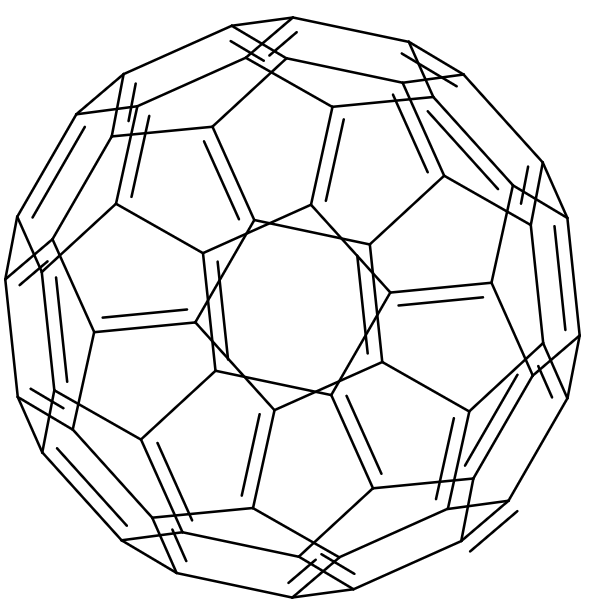
\includegraphics[width=6cm]{imagenes/Ant/c60.png}
  \caption{Representación esquemática del fulereno C\textsubscript{60}}
  \label{fig:jaula-c60}
\end{figure}


En la actualidad se reconoce que los fulerenos también se forman de manera natural en diversos procesos de alta temperatura que involucran materia carbonosa. Dado que las metodologías de síntesis masiva generan inevitablemente una mezcla heterogénea de fulerenos y otras nanoestructuras de carbono, el desarrollo tecnológico actual se enfoca en maximizar el rendimiento del hollín sintetizado, así como en optimizar los procesos de separación y purificación de especies específicas \cite{cavina2024orthoflaviviral}.


\subsection{Propiedades Fisicoquímicas y Estructura Cristalina del C\textsubscript{60}}

Los fulerenos son alótropos del carbono estructurados como poliedros huecos, esféricos u ovoides. Su nombre rinde homenaje a las cúpulas geodésicas de Sir R. Buckminster Fuller. El representante más común es el C\textsubscript{60} (buckminsterfulereno), una molécula con geometría de icosaedro truncado constituida por 60 vértices y 32 caras (20 hexagonales y 12 pentagonales) \textbf{véase la Figura \ref{fig:estructura-c60}}. En esta arquitectura, cada átomo de carbono presenta hibridación $sp^2$ y coordinación trigonal. La distancia media del enlace C--C, determinada mediante resonancia magnética nuclear (RMN), es de $1.44\ \text{\AA}$. Por su parte, los cuatro electrones de valencia de cada carbono forman dos enlaces simples y uno doble rico en electrones. Al satisfacer sus capas de valencia, el empaquetamiento molecular genera un sólido cristalino de van der Waals con propiedades aislantes o semiconductoras \cite{wilson2024role}.

\begin{figure}[H]
  \centering
  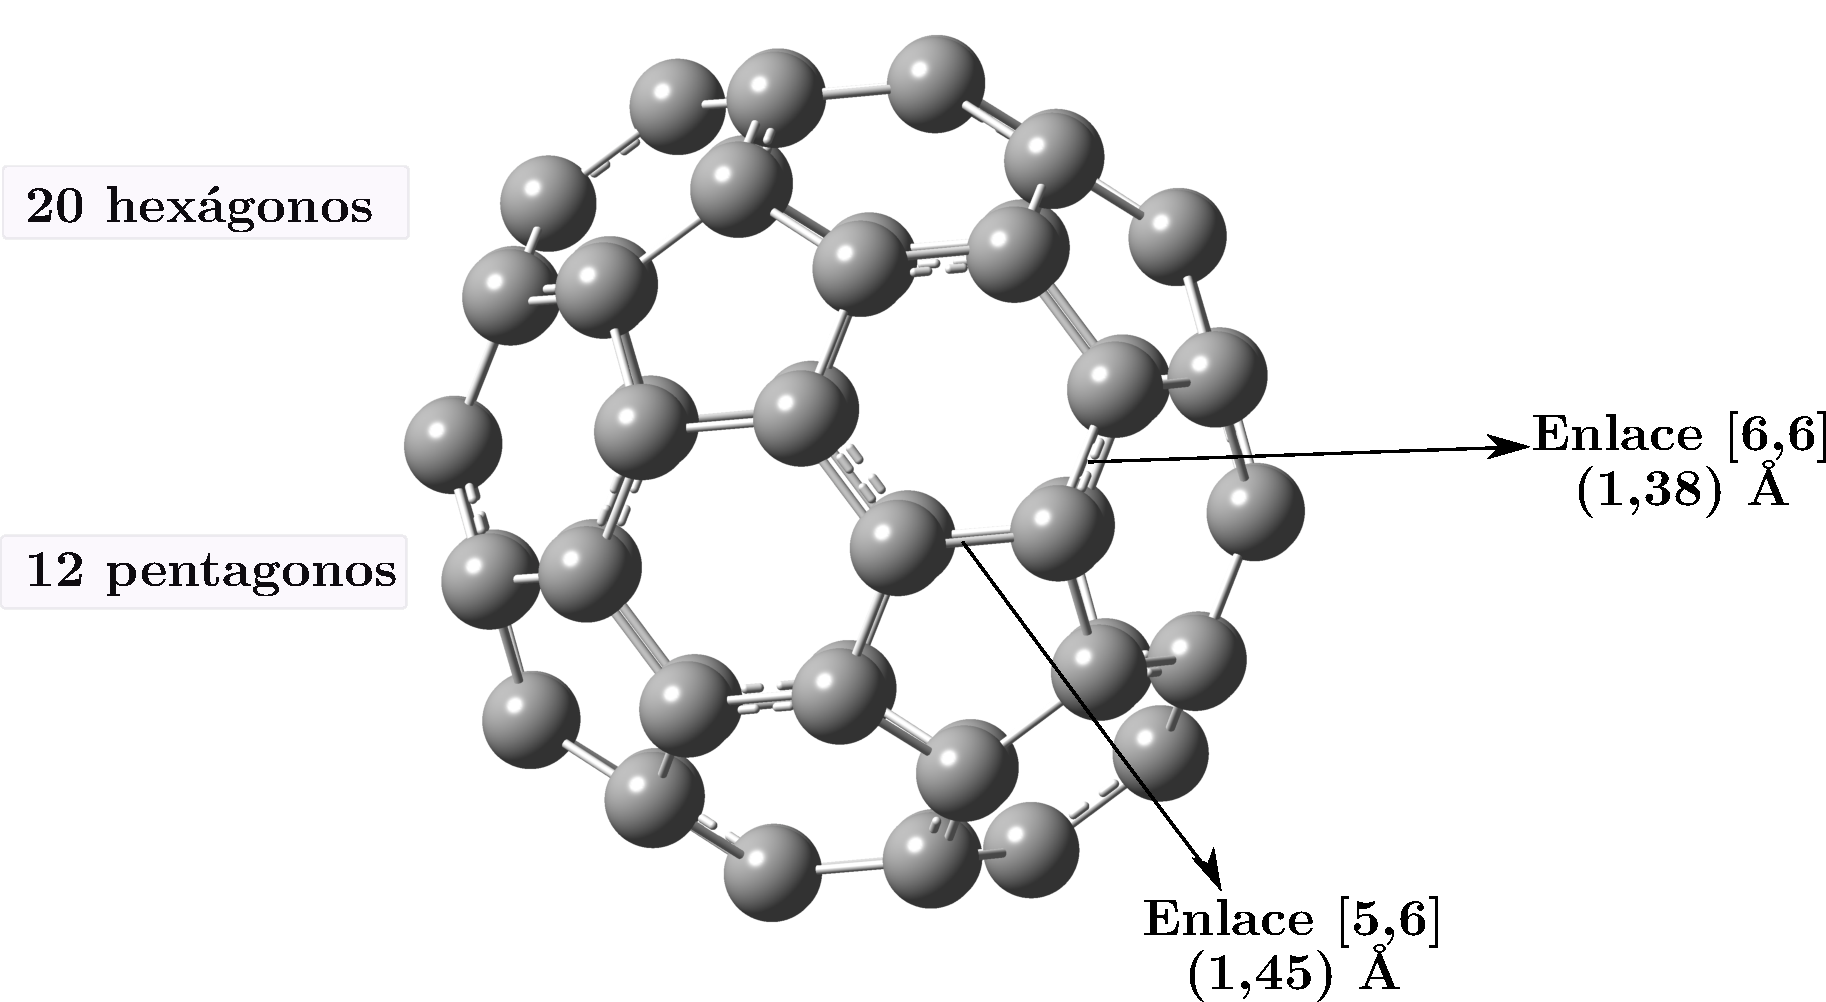
\includegraphics[width=15cm]{imagenes/Ant/c60.pdf}
  \caption{Representación esquemática de las principales formas alotrópicas del carbono}
  \label{fig:estructura-c60}
\end{figure}

En términos dimensionales, esta molécula posee un diámetro externo promedio de $0.7\text{ nm}$. Asimismo, está constituida por anillos aromáticos condensados que conforman un sistema $\pi$ totalmente extendido y conjugado \cite{nakamura2012water}.

La conformación de la jaula cerrada del C\textsubscript{60} requiere combinar caras pentagonales y hexagonales, principio sustentado por el teorema de Euler. Este teorema establece que se necesitan exactamente 12 pentágonos para cerrar la red polimérica, sin importar el número de hexágonos incorporados. Como los anillos pentagonales introducen una elevada tensión angular en la red de enlaces, la presencia de pentágonos adyacentes desestabiliza la estructura. Este fenómeno se formaliza en la Regla del Pentágono Aislado (IPR). Por esta razón, el C\textsubscript{60} representa la estructura más pequeña que alberga 12 pentágonos sin compartir aristas. No obstante, en los espectros de masas iniciales se detectó una señal destacada de C\textsubscript{28} (12 pentágonos y solo 2 hexágonos). A pesar de infringir la regla IPR, esta especie presenta una configuración electrónica inusualmente estable \cite{cavina2024orthoflaviviral}.

Debido a la elevada densidad de dobles enlaces disponibles para reaccionar con radicales libres, la estructura del C\textsubscript{60} se ha investigado ampliamente para aplicaciones biomédicas. Esta molécula exhibe propiedades antioxidantes excepcionales y cuenta con la capacidad de atravesar membranas celulares y la barrera hematoencefálica. Asimismo, logra modular el transporte iónico y presenta afinidad interfacial con bicapas lipídicas \cite{norshidah2023assessing}.

Por otra parte, una propiedad crítica en el diseño farmacológico es la lipofilia, la cual se evalúa mediante el coeficiente de reparto octanol-agua ($\log P_{\text{ow}}$). En este sentido, el C\textsubscript{60} prístino no modificado es altamente lipofílico, registrando un valor de $\log P_{\text{ow}} = 6.67$ \cite{sharoyko2021biologically}.

Como consecuencia de esta elevada lipofilia, las moléculas de fulereno puro son fuertemente hidrófobas. Por ello, resultan prácticamente insolubles en medios acuosos y fluidos biológicos \cite{marforio2021dissecting}.
\section{Estrategias de Funcionalización Química}

La funcionalización superficial de los nanomateriales de carbono (CNM) constituye una estrategia fundamental para optimizar su biodegradabilidad, perfil de seguridad y solubilidad en medios acuosos. La modificación de la superficie de los CNM permite generar un sistema dinámico al combinar diversos fármacos, péptidos, ácidos nucleicos, aminoácidos y proteínas. Este anclaje estratégico incrementa la eficiencia farmacológica y la solubilidad del compuesto, reduciendo de manera simultánea su citotoxicidad intrínseca. La incorporación de estos agentes funcionales se realiza mediante interacciones intermoleculares covalentes o no covalentes (iónicas, fuerzas de van der Waals y apilamiento $\pi$--$\pi$). Esta disposición facilita la localización dirigida en regiones específicas de la arquitectura nanométrica \cite{gaur2021biomedical}.

Por su parte, los fulerenos constituyen una familia de materiales hidrofóbicos integrados exclusivamente por átomos de carbono dispuestos en forma de poliedros huecos \cite{sharoyko2021biologically}. % Nota bibliográfica original pendiente de correspondencia: (18)
 Desde su aislamiento en 1990, la química de los fulerenos ha experimentado una profunda evolución. De este modo, se ha demostrado su capacidad para interactuar con diversos solutos en entornos ambientales y sistemas biológicos, ejerciendo efectos significativos sobre el metabolismo, el transporte y la reactividad celular \cite{ chang2024recent, bai2024research}. Sin embargo, la molécula de C\textsubscript{60} carece intrínsecamente de una solubilidad acuosa adecuada ($< 10^{-11}\ \text{g/L}$), lo que induce su rápida agregación coloidal en medios fisiológicos. Para superar esta limitación crítica se emplean principalmente dos metodologías:\cite{sosnowska2019mechano}.

\begin{itemize}
    \item \textbf{Complejación no covalente:} Utilización de agentes solubilizantes para enmascarar parcialmente la superficie hidrófoba de la jaula de carbono.
    \item \textbf{Funcionalización covalente:} Modificación química directa sobre los dobles enlaces de la superficie del fulereno.
\end{itemize}

En este contexto, la síntesis de derivados de fulereno (FD) mediante la adhesión covalente de fracciones hidrofílicas se ve favorecida por la elevada curvatura del C\textsubscript{60} y su extenso sistema de electrones $\pi$ conjugados. Esta elevada reactividad química permite acoplar cadenas laterales hidrofílicas, anfifílicas o estructuras de anillos fusionados al núcleo esférico, transformando a los fulerenos en versátiles bloques de construcción nanométricos. Al incorporar estas cadenas, los derivados pueden conservar o potenciar su capacidad para generar oxígeno singlete ($^1\text{O}_2$), radicales hidroxilo ($\cdot\text{OH}$) y aniones superóxido ($\text{O}_2^{\bullet-}$). Asimismo, este proceso incrementa el momento dipolar y favorece la estabilidad coloidal en disolventes polares \cite{gaur2021biomedical}.

Se ha establecido que los derivados del C\textsubscript{60} poseen energías de reorganización sumamente pequeñas durante los procesos de transferencia electrónica. Esta propiedad los convierte en aceptores de electrones ideales para aplicaciones biomédicas y energéticas. \cite{sharoyko2021biologically, nelson2022principios}. En los últimos años, el desarrollo de enfoques sintéticos avanzados ha permitido obtener aductos de fulereno con solubilidades acuosas fisiológicamente aceptables, alcanzando concentraciones de entre 10 y $200\ \text{mg/mL}$ o superiores. % Nota bibliográfica original pendiente de correspondencia: (28)
 Gracias a estas características, los fulerenos funcionalizados destacan en cosmetología, ciencia de materiales, electroquímica y sistemas de liberación controlada de fármacos \cite{andrada2012nanotecnologia, liu2024quantum}. La diversificación de sus aductos solubles en agua incluye fulerenoles, carboxifulerenos y conjugados con aminoácidos. Estos compuestos destacan por presentar actividad antioxidante, antimicrobiana, neuroprotectora, radioprotectora, así como su uso como fotosensibilizadores en terapia fotodinámica e inhibidores enzimáticos \cite{marforio2021dissecting}.

\subsubsection{Fulereno con Glicina (C\textsubscript{60}--Gly): Síntesis y Caracterización Estructural}

A diferencia de otros aminoácidos estándar cuyo carbono $\alpha$ constituye un centro quiral, la glicina (Gly) es el aminoácido estructuralmente más simple y carece de quiralidad. Aunque formalmente se clasifica como apolar, su diminuta cadena lateral —constituida por un único átomo de hidrógeno— no genera impedimento estérico ni aporta una contribución hidrofóbica significativa \cite{bolshakova2023facile}. Por su parte, los conjugados de fulereno con aminoácidos (fulleroaminoácidos) resultan de elevado interés biomédico. Esto se debe a que la fracción funcionalizadora aporta hidrofilia y biocompatibilidad, al tiempo que conserva importantes actividades biológicas útiles en la administración de fármacos antitumorales, neuroprotectores, antioxidantes y antivirales \cite{jiang2015synthesis}.

Los aminoácidos destacan como ligandos idóneos para modificar la jaula de C\textsubscript{60} gracias a la presencia de sus grupos polares carboxilo (--COOH) y amino (--NH\textsubscript{2}). En el caso de la glicina, su reducido volumen molecular minimiza el impedimento estérico. Al mismo tiempo, la elevada nucleofilia de su grupo amino terminal facilita su unión mediante un ataque nucleofílico directo sobre los dobles enlaces electrófilos del C\textsubscript{60} \textbf{véase la Figura \ref{Fig:estructura_c60_gly}}\cite{jiang2015synthesis}. Recientemente, se reportó la síntesis del aducto tetrasustituido de C\textsubscript{60} funcionalizado con glicina, denominado C\textsubscript{60}--Gly [\ce{C\textsubscript{60}(C2H4NO2)4}], el cual alcanzó un rendimiento sintético del 85\% y una pureza cromatográfica del 99.8\%. % Nota bibliográfica original pendiente de correspondencia: (50)
 La estructura química del aducto C\textsubscript{60}--Gly se representa a continuación. 

\begin{figure}[htbp]
  \centering
  \IfFileExists{Imagenes/Ant/estructura_c60_gly.png}{
    \includegraphics[width=0.65\textwidth]{Imagenes/estructura_c60_gly.png}
  }{
    \fbox{\parbox[c][4.5cm][c]{0.65\textwidth}{\centering Imagen pendiente: estructura química del aducto tetrasustituido de C\textsubscript{60} con glicina.}}
  }
  \caption{Estructura química del aducto de fulereno C\textsubscript{60} funcionalizado con glicina (C\textsubscript{60}--Gly). \cite{sharoyko2024modification}}
  \label{Fig:estructura_c60_gly}
\end{figure}

% Nota bibliográfica original pendiente de correspondencia: (50)
 La caracterización espectroscópica mediante Resonancia Magnética Nuclear de Carbono-13 (\textsuperscript{13}C RMN) confirma de manera inequívoca el enlace covalente a la jaula esférica. El espectro de \textsuperscript{13}C RMN del aducto C\textsubscript{60}--Gly exhibe desplazamientos químicos característicos a $177\text{ ppm}$ ($a$, carbono carboxílico), $144\text{ ppm}$ (núcleo de $sp^2$-C\textsubscript{60}), $65\text{ ppm}$ ($c$, $sp^3$-$C$ de la jaula enlazado al grupo amino), $50\text{ ppm}$ ($b$, grupo metileno --CH\textsubscript{2}--) y $17\text{ ppm}$ ($d$, $sp^3$-$C$ unido a hidrógeno). 

\begin{figure}[H]
  \centering
  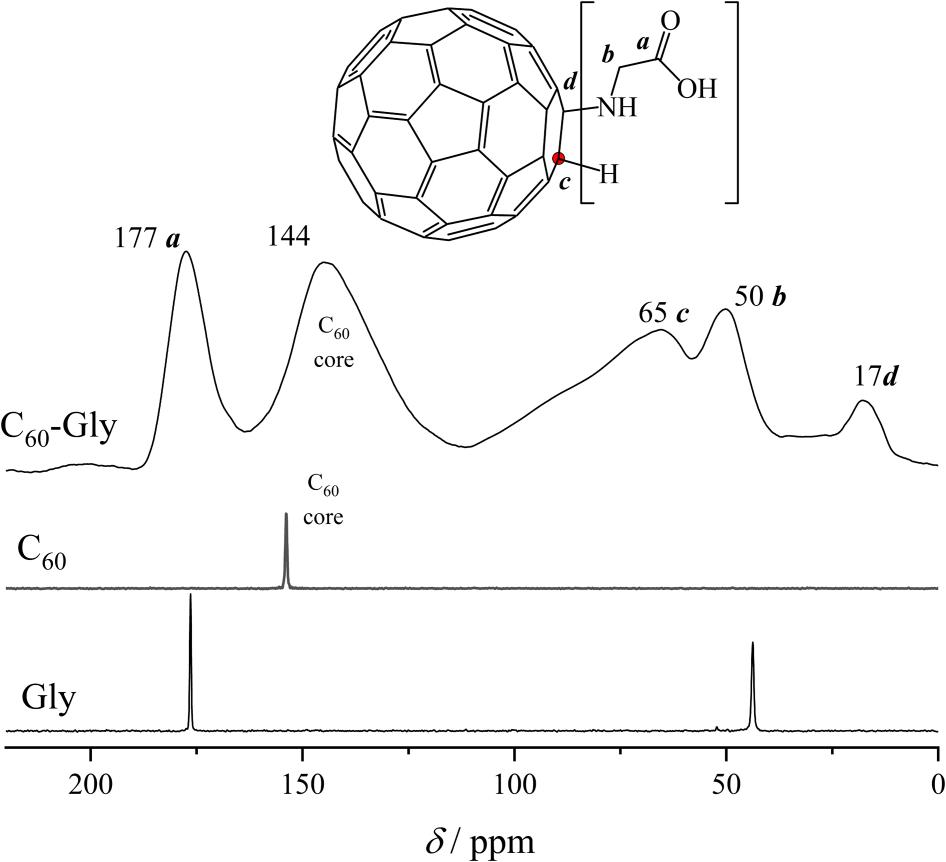
\includegraphics[width=11cm]{imagenes/Ant/NMR.png}
  \caption{Espectro de RMN de \textsuperscript{13}C y asignación de señales estructurales del aducto C\textsubscript{60}--Gly.}
  \label{Fig:rmn_c60_gly}
\end{figure}

Desde la perspectiva fisicoquímica, el aducto C\textsubscript{60}--Gly presenta un coeficiente de partición de $\log P_{\text{ow}} = 0.25$. Este valor evidencia una afinidad equilibrada tanto por fases acuosas como lipídicas, lo que contrasta con la extrema hidrofobicidad del C\textsubscript{60} prístino ($\log P_{\text{ow}} = 6.67$). % Nota bibliográfica original pendiente de correspondencia: (50)
 En disolución acuosa, el aducto se autoasocia en nanoagregados coloidales de 30 a $50\text{ nm}$ con un potencial zeta ($\zeta$) de $-40$ a $-30\text{ mV}$, lo que asegura una elevada estabilidad coloidal por repulsión electrostática \cite{sharoyko2024modification}. Sus principales propiedades y parámetros estructurales se resumen en la Tabla~\ref{tab:aplicaciones_fullereno}. \cite{nakamura2012water,jiang2015synthesis,sharoyko2024modification}.

\begin{table}[H]
\centering
\caption{Propiedades fisicoquímicas y estructurales del aducto C\textsubscript{60}--Gly (Fulereno--Glicina) para aplicaciones biomédicas.}
\label{tab:aplicaciones_fullereno}
\begin{tabular}{l p{10cm}}
\toprule
\textbf{Característica / Parámetro} & \textbf{Descripción del aducto C\textsubscript{60}--Gly} \\
\midrule
Estequiometría y pureza & Tetra-aducto \ce{C\textsubscript{60}(C2H4NO2)4} (Rendimiento: 85\%, Pureza: 99.8\%).\\
Geometría del ligando & Sin cadena lateral voluminosa; impedimento estérico mínimo. \\
Grupos funcionales terminales & Grupos amino (--NH\textsubscript{2}) e hidroxilo/carboxilo (--COOH) libres. \\
Perfil de lipofilia ($\log P_{\text{ow}}$) & $\log P_{\text{ow}} = 0.25$ (carácter anfifílico equilibrado). \\
Comportamiento coloidal & Nanoasociados ($30\text{--}50\text{ nm}$) con alta estabilidad ($\zeta = -40\text{ a }-30\text{ mV}$). \\
Seguridad biológica & Alta hemocompatibilidad, baja citotoxicidad e inhibición de agregación plaquetaria  \cite{sharoyko2024modification}. \\
\bottomrule
\end{tabular}
\end{table}

La superficie del fulereno prístino presenta regiones con deficiencia electrónica (agujeros $\pi$), las cuales establecen interacciones anión--$\pi$ con residuos cargados negativamente. Asimismo, interactúa mediante apilamiento $\pi$--$\pi$ con residuos aromáticos (Trp, Phe, Tyr, His) y mediante interacciones hidrofóbicas con residuos alifáticos (Leu, Val, Pro, Ile, Ala, Met). Por su parte, las cadenas laterales catiónicas (Arg, Lys) forman interacciones catión--$\pi$ sustancialmente más fuertes que los residuos neutros (Asn, Gln). Adicionalmente, la densidad electrónica de la jaula le permite actuar como aceptor de puentes de hidrógeno no estándar. % Nota bibliográfica original pendiente de correspondencia: (30)
 Los principales tipos de interacciones intermoleculares se resumen a continuación (véase la Tabla~\ref{tab:interacciones_fullereno}) \cite{bolshakova2023facile}.

\begin{table}[H]
\centering
\caption{Principales tipos de interacciones intermoleculares entre la superficie de fulerenos y residuos aminoacídicos en estructuras proteicas.}
\label{tab:interacciones_fullereno}
\begin{tabular}{l l}
\toprule
\textbf{Tipo de Interacción} & \textbf{Mecanismo / Residuos Involucrados} \\
\midrule
Apilamiento $\pi$--$\pi$ & Residuos aromáticos (Trp, Phe, Tyr, His) \\
Interacciones hidrofóbicas & Residuos alifáticos (Leu, Val, Pro, Ile, Ala, Met) \\
Interacciones catión--$\pi$ & Cadenas con carga positiva (Arg, Lys) \\
Interacciones anión--$\pi$ & Residuos cargados negativamente / Agujeros $\pi$ \\
Puentes de hidrógeno & Enlaces no estándar en regiones ricas en $e^-$ \\
Efecto tipo surfactante & Cadenas anfifílicas y polares \\
\bottomrule
\end{tabular}
\end{table}

\section{Química Cuántica y Teoría del Funcional de la Densidad (DFT)}
La Teoría del Funcional de la Densidad (DFT) se fundamenta en que la densidad electrónica del estado fundamental, $\rho(\vec{r})$, es la variable fundamental para describir la energía y las propiedades electrónicas de un sistema multielectrónico en su estado fundamental. En este marco formal, la energía total del sistema $E[\rho]$ se expresa como un funcional de $\rho(\vec{r})$, donde el término de intercambio y correlación $E_{\text{xc}}[\rho]$ compensa las diferencias de energía cinética e interacciones interelectrónicas entre el sistema real interactuante y un sistema de referencia ficticio de electrones no interactuantes (Kohn-Sham). Por su parte, el modelado \textit{in silico} mediante DFT permite optimizar la geometría molecular ajustando las coordenadas atómicas —como longitudes, ángulos de enlace y ángulos de torsión— hasta lograr la minimización de la superficie de energía potencial \cite{kohn1965self}.

Para el estudio de aductos de fulereno C\textsubscript{60} funcionalizados con aminoácidos, la elección del funcional y la base es determinante para equilibrar el costo computacional y la precisión electrónica. El funcional híbrido B3LYP combina el intercambio exacto de Hartree-Fock con los funcionales de intercambio de Becke (B3) y la correlación de Lee-Yang-Parr (LYP), estando ampliamente validado para la caracterización de nanoestructuras carbonosas. Por otro lado, el conjunto de bases polarizado triple-zeta 6-311G(d,p) emplea 6 funciones gaussianas primitivas para los electrones del núcleo (\textit{core}) y triplica la descripción de los orbitales de valencia, añadiendo funciones $d$ en átomos pesados y $p$ en átomos de hidrógeno. Esta combinación resulta idónea para mapear transferencias de carga, momentos dipolares y densidades electrónicas en intermediarios monocarboxilados y poliderivados \cite{nikolaev2020thermodynamic, mico2024estudio}.

 Mediante una aproximación basada en los orbitales frontera, los niveles energéticos del orbital ocupado de mayor energía ($E_{\text{HOMO}}$) y del orbital desocupado de menor energía ($E_{\text{LUMO}}$) permiten cuantificar los descriptores globales de reactividad química. El potencial de ionización ($I$) y la afinidad electrónica ($A$) se aproximan según:
\begin{equation}
I \approx -E_{\text{HOMO}}
\end{equation}
\begin{equation}
A \approx -E_{\text{LUMO}}
\end{equation}

Asimismo, la DFT permite explorar la reactividad local de una molécula a través de las funciones de Fukui (FF). Estas funciones, derivadas mediante esquemas de diferencias finitas ($\Delta N = \pm 1$), identifican los sitios atómicos propensos a ataques nucleofílicos ($f^+$), electrófilos ($f^-$) o por radicales libres ($f^0$):
\begin{equation}
f^+(\vec{r}) = \rho_{\text{anión}}(\vec{r}) - \rho_{\text{neutro}}(\vec{r}) \quad \text{(Ataque nucleofílico / Regiones electrófilas)}
\end{equation}
\begin{equation}
f^-(\vec{r}) = \rho_{\text{neutro}}(\vec{r}) - \rho_{\text{catión}}(\vec{r}) \quad \text{(Ataque electrófilo / Regiones nucleofílicas)}
\end{equation}
\begin{equation}
f^0(\vec{r}) = \frac{\rho_{\text{anión}}(\vec{r}) - \rho_{\text{catión}}(\vec{r})}{2} \quad \text{(Ataque por radicales libres)}
\end{equation}
Estas aproximaciones orbitales no equivalen a calcular diferencias de energía total entre estados con distinto número de electrones. En particular, la estimación de la afinidad electrónica a partir del LUMO debe interpretarse con cautela.

En aductos de C\textsubscript{60} funcionalizados con aminoácidos (como L-arginina o glicina), los cálculos indican que los átomos de carbono del núcleo enlazados al aminoácido ceden densidad electrónica hacia los átomos de nitrógeno adyacentes. Este reordenamiento polariza localmente la jaula, permitiendo la formación de interacciones intermoleculares selectivas tanto por el núcleo hiperconjugado como por las cadenas laterales de los residuos \cite{moncada2008caracterizacion, gaur2021biomedical}.

\subsection{Acoplamiento Molecular, Dinámica Molecular y Evaluación de Actividad Biomédica}
El acoplamiento molecular permite predecir los modos de unión óptimos y las afinidades de enlace entre aductos de fulereno y dianas proteicas de relevancia clínica. Empleando herramientas como AutoDock Vina, se parametrizan rejillas tridimensionales (cajas de delimitación) centradas en bolsillos catalíticos o alostéricos. De este modo, se evalúan formas abiertas y cerradas de enzimas clave como la proteasa NS2B-NS3 del virus del dengue (DENV-2), la proteína tirosina fosfatasa 1B (PTP1B) o la proteasa del VIH-1. Las interacciones se estabilizan mediante el acomodamiento hidrofóbico de la jaula en la cavidad no polar, interacciones catión--$\pi$ con cadenas laterales básicas (Arg, Lys) y puentes de hidrógeno dirigidos por las fracciones carboxilo y amino terminales del aminoácido acoplado \cite{nelson2022principios,jiang2015synthesis, wang2024strain}.

Por su parte, la dinámica molecular (DM) profundiza en la estabilidad temporal y la flexibilidad conformacional de los complejos ligando-proteína. Utilizando entornos de cómputo como GROMACS y campos de fuerza como GROMOS96 (53A6) —con topologías de ligando parametrizadas vía servidores como ATB y cargas atómicas cuánticas—, el sistema se solvata en modelos de agua explícita (por ejemplo, SPC) e iones de neutralización ($\text{Na}^+/\text{Cl}^-$). Tras la minimización energética por descenso más pronunciado, el sistema se somete a fases de equilibrado isocórico-isotérmico (NVT, $300\text{ K}$) e isotérmico-isobárico (NPT, $1.0\text{ bar}$) mediante acoplamientos de temperatura (V-rescale) y presión (Parrinello-Rahman). La energía libre de unión ($\Delta G_{\text{bind}}$) se cuantifica posteriormente a través de métodos de disolvente continuo (\textit{Continuum Solvent}) como MM/GBSA (\textit{Molecular Mechanics/Generalized Born Surface Area}) en paquetes como AMBER, desglosando las contribuciones entálpicas y electrostáticas residuo por residuo \cite{nelson2022principios, liu2023fullerene}.

La integración del modelado \textit{in silico} respalda de manera directa el potencial biomédico de los fulerenos funcionalizados en diversas patologías humanas. Gracias a su extensa red de electrones $\pi$, el C\textsubscript{60} funcionalizado actúa como una ``esponja de radicales libres'', atrapando especies reactivas de oxígeno (ROS) e inhibiendo el estrés oxidativo involucrado en el daño tisular y neurodegenerativo (enfermedades de Alzheimer y Parkinson). Asimismo, las simulaciones demuestran que las interacciones electrostáticas e hidrofóbicas entre los aductos hidrofílicos y los oligómeros del péptido $\beta$-amiloide ($\text{A}\beta$) o la $\alpha$-sinucleína alteran el autoensamblaje fibrilar, deteniendo la polimerización neurotóxica. En terapias fotodinámicas (PDT) y patógenos infecciosos, estos derivados generan la fotoinactivación de microorganismos y la rotura de membranas bacterianas, mostrando una biocompatibilidad dependiente de la dosis y de la arquitectura sintética del aducto \cite{wilson2024role, wang2024strain,  celaya2022administracion, partha2009biomedical}.
  



















\titleformat{\chapter}[display]
  {\normalfont\bfseries}{}{0pt}{\Large} % Este comando es para eliminar la aparición de "Capítulo N" en el PDF. Para emplear el formato de la tesis simplemente eliminamos la línea. 
\chapter{Planteamiento del Problema}
\justifying
El dengue sigue siendo un problema de salud pública sin antivirales específicos realmente eficaces. La proteasa NS2B-NS3 del DENV-2 es un blanco terapéutico clave y los fulerenos funcionalizados con aminoácidos son plataformas prometedoras al mejorar su solubilidad y estructura electrónica. Aún se desconoce cómo estas modificaciones afectan su interacción con NS2B-NS3, por lo que estudiarlas puede aportar bases para diseñar nuevos inhibidores contra el dengue.
\begin{center}
\fcolorbox{AzulOscuro!30}{GrisClaro}{
            \begin{minipage}{0.9\textwidth}
                \small
               ¿Cómo afecta la funcionalización de fulerenos con aminoácidos a su estructura electrónica y qué impacto tiene en su interacción con la proteína del dengue NS2B-NS3 correspondiente al serotipo DENV-2?
            \end{minipage}
        }
  \end{center}
  
\begin{center}
  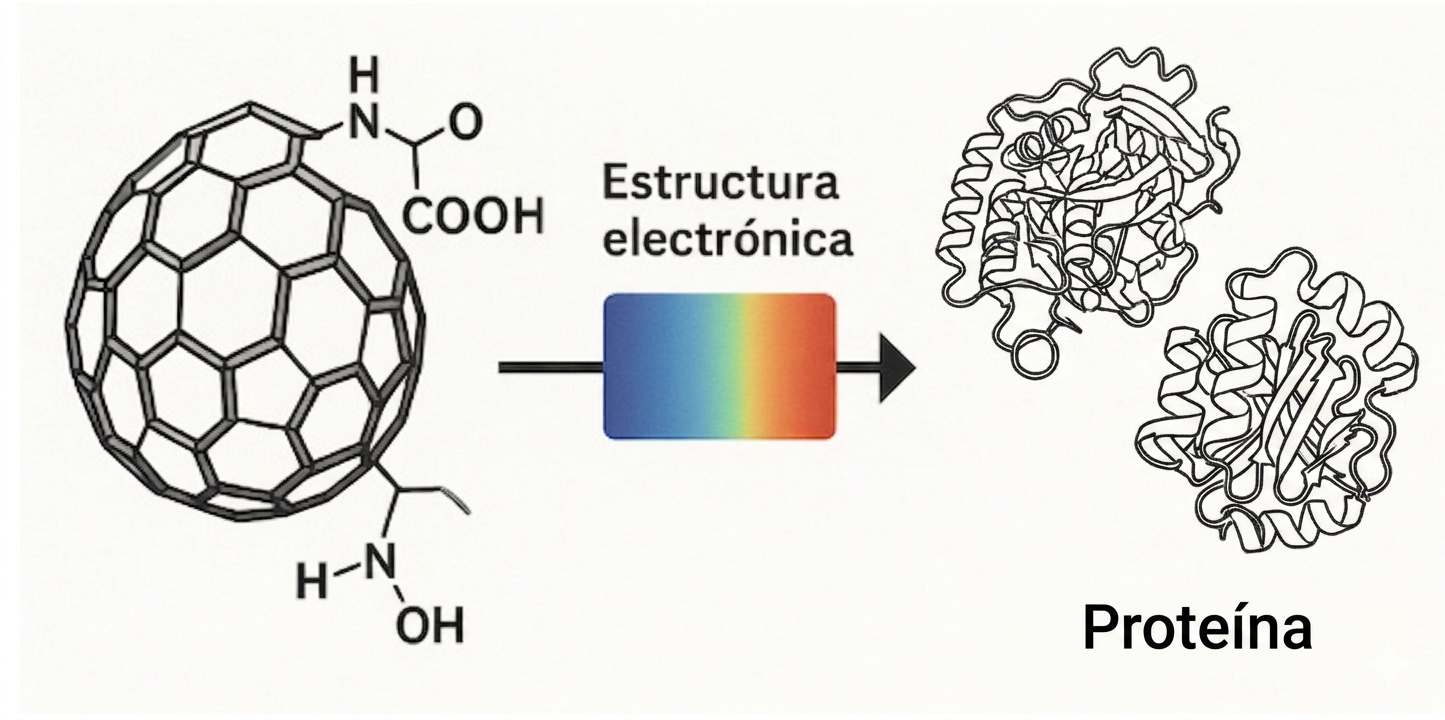
\includegraphics[width=0.6\textwidth,height=0.3\textwidth]{Contenido/Plan/planteamiento-1.png}
\end{center}



\titleformat{\chapter}[display]
  {\normalfont\bfseries}{}{0pt}{\Large} % Este comando es para eliminar la aparición de "Capítulo N" en el PDF. Para emplear el formato de la tesis simplemente eliminamos la línea. 
\chapter{Justificación}
Los fulerenos, reconocidos por sus propiedades estructurales y electrónicas únicas, han captado un interés creciente en el ámbito de las aplicaciones biomédicas. Sin embargo, su baja solubilidad en entornos acuosos y fisiológicos constituye un obstáculo crítico que limita significativamente su aplicación directa y su potencial terapéutico.

Para superar esta restricción, la funcionalización química de la superficie del fulereno mediante la adición de aminoácidos, como la glicina, representa una estrategia eficaz. Esta modificación no solo incrementa la solubilidad del sistema en medios biológicos, sino que también mejora su capacidad de interacción y afinidad hacia dianas macromoleculares.

En este contexto, la implementación de herramientas computacionales de modelado, reactividad y acoplamiento molecular proporciona una comprensión detallada a nivel atómico de los mecanismos de interacción del sistema. De este modo, el presente trabajo contribuye al diseño racional de aductos funcionalizados dirigidos específicamente contra la proteasa NS2B-NS3 del virus del dengue, ofreciendo bases teóricas para el desarrollo de nuevos agentes con potencial biomédico.
\titleformat{\chapter}[display]
  {\normalfont\bfseries}{}{0pt}{\Large} % Este comando es para eliminar la aparición de "Capítulo N" en el PDF. Para emplear el formato de la tesis simplemente eliminamos la línea. 
\chapter{Hipótesis}
La funcionalización de fulerenos con aminoácidos modifica su estructura electrónica, aumentando su solubilidad y reactividad, lo que mejora su interacción con biomoléculas y potencia su actividad para el acoplamiento con la diana terapéutica del serotipo 2 de NS2B-NS3 correspondiente al virus del dengue.

\titleformat{\chapter}[display]
  {\normalfont\bfseries}{}{0pt}{\Large} % Este comando es para eliminar la aparición de "Capítulo N" en el PDF. Para emplear el formato de la tesis simplemente eliminamos la línea. 
\chapter{Objetivos}

\section{Objetivo General}
Identificar las estructuras más estables del derivado C\textsubscript{60}(Gly)\textsubscript{4} y analizar su interacción con las proteínas NS2B-NS3 en conformación abierta  del serotipo DENV-2.

\section{Objetivos Particulares}

\begin{enumerate}
    \item Evaluar los sitios de adición del aminoácido glicina en la estructura del fulereno C\textsubscript{60}.
    \item Valorar la solubilidad, reactividad química y capacidad de interacción del fulereno funcionalizado.
    \item Identificar los sitios de acoplamiento del C\textsubscript{60}(Gly)\textsubscript{4} con la proteína correspondiente al serotipo DENV-2.
    \item Encontrar la relación entre la teoría y las tendencias experimentales a partir de resultados teóricos.
\end{enumerate}


\titleformat{\chapter}[display]
  {\normalfont\bfseries}{}{0pt}{\Large} % Este comando es para eliminar la aparición de "Capítulo N" en el PDF. Para emplear el formato de la tesis simplemente eliminamos la línea. 
\chapter{Materiales y Métodos}
\section{Construcción y optimización del sistema C\textsubscript{60}(Gly)\textsubscript{4}}
La construcción de la estructura tridimensional del aducto C\textsubscript{60}(Gly)\textsubscript{4} se llevó a cabo utilizando el visualizador y editor molecular GaussView, tomando como referencia la metodología reportada por Sharoyko y colaboradores. La optimización de las geometrías moleculares se realizó mediante la teoría del funcional de la densidad (DFT) empleando el nivel de teoría B3LYP/6-311G(d,p). Para confirmar que las estructuras optimizadas corresponden a un mínimo local real en la superficie de energía potencial (SEP), se realizaron los cálculos de frecuencias vibracionales, verificando la ausencia de frecuencias imaginarias.
\section{Determinación de la reactividad local}
Para determinar los sitios preferenciales de adición para un ataque nucleofílico del grupo amino de la glicina sobre la jaula de C\textsubscript{60}, se calcularon las Funciones de Fukui (FF) como descriptores de reactividad local. Dado que la glicina actúa como especie nucleofílica a través de su grupo amino y la jaula de C\textsubscript{60} se comporta como el electrófilo, se evaluó la Función de Fukui para ataques nucleofílicos ($f^+$). 

La reactividad local se describe mediante las funciones de Fukui. En su representación espacial, la aproximación por diferencias finitas se expresa de la siguiente manera:

\begin{equation}
    \text{Ataque nucleofílico: } f^+(\mathbf{r}) = \rho_{N+1}(\mathbf{r}) - \rho_N(\mathbf{r})
\end{equation}

\begin{equation}
    \text{Ataque electrofílico: } f^-(\mathbf{r}) = \rho_N(\mathbf{r}) - \rho_{N-1}(\mathbf{r})
\end{equation}

\begin{equation}
    \text{Ataque radicalario: } f^0(\mathbf{r}) = \frac{1}{2} \left[ \rho_{N+1}(\mathbf{r}) - \rho_{N-1}(\mathbf{r}) \right]
\end{equation}

En estas expresiones, $\rho_{N+1}(\mathbf{r})$, $\rho_N(\mathbf{r})$ y $\rho_{N-1}(\mathbf{r})$ representan la densidad electrónica en la posición espacial $\mathbf{r}$ para las especies en sus estados aniónico ($N+1$), neutro ($N$) y catiónico ($N-1$), respectivamente. Estas funciones espaciales deben distinguirse de los índices condensados a átomos, cuya obtención depende del esquema de partición de la densidad electrónica. El esquema empleado en este estudio queda pendiente de documentar con las salidas de cálculo.

El procedimiento de adición del aminoácido sobre la jaula de C\textsubscript{60} se llevó a cabo de manera iterativa. Se identificaron los átomos de carbono con los mayores valores del índice $f_k^+$, y se adicionó la siguiente molécula de glicina en el carbono con la reactividad más pronunciada para posteriormente optimizar la geometría, repitiendo este protocolo para cada etapa de adición de un nuevo aminoácido.

Las propuestas estructurales se optimizaron mediante la teoría del funcional de la densidad (DFT) empleando el nivel de teoría B3LYP/6-311G(d,p), y se corroboró la ausencia de frecuencias imaginarias mediante el análisis de frecuencias vibracionales para asegurar que correspondieran a mínimos locales en la superficie de energía potencial. La comparación de las propuestas estructurales se realizó mediante sus diferencias de energía relativa. Las configuraciones evaluadas y las seleccionadas para continuar la funcionalización se presentan en Resultados, hasta obtener el aducto C\textsubscript{60}(Gly)\textsubscript{4}.
\section{Evaluación de la reactividad global y mapa de potencial electrostático}
Se evaluaron los descriptores de reactividad global para analizar la facilidad del aducto para donar o aceptar electrones y su relación con un posible comportamiento antioxidante. Para ello, se calcularon las energías del sistema en sus estados neutro, aniónico y catiónico, lo que permitió obtener el potencial de ionización ($I$) y la afinidad electrónica ($A$). Estos parámetros permitieron caracterizar la susceptibilidad y predisposición del sistema a reaccionar ante diversas especies químicas.

Para identificar los sitios propensos a interacciones electrostáticas, se generó la superficie de mapa de potencial electrostático (MEP, por sus siglas en inglés) para el ligando C\textsubscript{60}(Gly)\textsubscript{4}. El MEP evalúa la distribución de carga eléctrica sobre una superficie de densidad electrónica constante alrededor de la molécula. La visualización se realizó mediante un código de colores estándar: las regiones rojas representan potencial negativo (zonas ricas en electrones o de carácter nucleofílico), las regiones azules representan potencial positivo (zonas deficientes en electrones o de carácter electrófilo) y las regiones verde-amarillas indican zonas con potencial cercano a cero en la escala de representación utilizada. De esta manera, se determinaron los sitios clave de la molécula capaces de establecer interacciones por fuerzas electrostáticas con el entorno proteico.

\section{Acoplamiento molecular}Para explorar el potencial inhibidor del sistema de fulereno C\textsubscript{60} funcionalizado con 4 glicinas sobre la proteína de replicación del virus del dengue (complejo NS2B-NS3) en su conformación abierta e inactiva, se llevó a cabo la reconstrucción y completación de la estructura utilizando la plataforma CHARMM-GUI. A partir de la estructura cristalográfica obtenida del Protein Data Bank (PDB ID: 2FOM), se modelaron los residuos no definidos correspondientes a los extremos N- y C-terminales. La calidad geométrica del modelo se evaluó mediante un mapa de Ramachandran, verificando los ángulos de torsión permitidos ($\phi$ y $\psi$) en la cadena principal. Posteriormente, la estructura se sometió a una minimización de energía empleando el campo de fuerza GROMOS 54A7 en el programa GROMACS.

El modelo resultante se preparó para el acoplamiento molecular a través de la interfaz AutoDockTools. Durante este proceso, se eliminaron las moléculas de agua cristalográficas, se añadieron los hidrógenos polares necesarios y se asignaron las cargas parciales de tipo Kollman. Asimismo, se revisaron manualmente los residuos sin carga asignada para corregir posibles desbalances energéticos antes de exportar la estructura en formato PDBQT.

Finalmente, se definió una caja de grilla (\textit{grid box}) centrada en la región de interés con los parámetros ajustados para la simulación. Para el análisis posterior de las conformaciones, se estableció un umbral de tolerancia de RMSD de 8 Å para el agrupamiento de las poses, determinado a partir de la visualización estructural del complejo proteína-ligando.
\section{Simulaciones de Acoplamiento Molecular con AutoDock Vina}
Las simulaciones de acoplamiento molecular (\textit{docking}) se llevaron a cabo utilizando el software AutoDock Vina. Las estructuras del receptor y los ligandos se prepararon y definieron en formato PDBQT. La ejecución del programa generó un total de 100 poses conformacionales, cada una asociada a su respectiva energía de afinidad de unión. Para la separación y gestión individual de estas conformaciones, se utilizó la herramienta \texttt{vina\_split}.

A partir de las conformaciones obtenidas, se realizó un análisis visual y un agrupamiento (\textit{clustering}) en función de su energía relativa, aplicando un umbral de corte basado en la Desviación Cuadrática Media (RMSD). Finalmente, se construyeron los histogramas de distribución para evaluar las poses comprendidas dentro de dicho umbral de tolerancia en concordancia con sus correspondientes valores de energía de unión.


%La estructura tridimensional de la proteina (2FOM) se obtuvo por medio de la base de datos protein data bank. La generacion de los parametros de topología se llevarona cabo mediante el software Gromacs(), empleando el campo de fuerza GROMOS96 53A6.
% BORRADOR PREVIO: conservado para cotejo; contiene parámetros contradictorios
% con los apartados siguientes y campos sin completar.
% Construccion del entorno de misulacion y minimización de energía 
% La proteina se ubico en el centro de una caja de simulacion respetando una distancia minina de () nm entre la superficie de la proteina y el limite de la caja. El entorno se solvató utilizando el modelo de agua () para posteriormente añadir contraiones neutralizantes Cl- o Na+. A continuacuib, se ejecuto una minimización de energía mediante el algoritmo de (steepest descent)
% %Fase de equilibrio 
% El sistema se equilibro en dos estapas bajo ciertas restricciones: Primero una fase (nvt) empleando el termostato V-rescale/Berendsen donde el volumen es constante a 300K durante 10 ns, este  y el segundo una fase en el conjunto isotérmico-isobárico  (npt) donde la presion es constante a 300K durante 10 ns utilizando el barostato Parrinello-Rahman., el cual ajusta dinamicamente el tamaño y la forma de la caja de simulación en respeusta a las fluctuaciones de la presion. Este mecanismo permite que el volumen del sistema se expanda o contraiga de manera anisotropica hasta alcanzar una presion promedio (1atm), simulando asi un entorno mas realista y flexible, como el que se encuetra en los sistemas biologicos. 
% 
% Una vez completadas las fases de equilibrio, se procedio con la simulación de producción por un total de 100ns, empleando un paso de integracion de 0.0015ps y un total de 66,666,6667 pasos. Durante esta etapa, los enlaces covalentes que involucran atomos de hidrogeno se restringieron mediante el algoritmo LIBCS, el cual permite mantener fijas estas distancias sin afectar la dinámica general del sistema. 
% 
% Se almacenaron las trayectorias y coordenadas para su posterior análisis estructural. Asimismo, se eliminaron las moleculas de agua y los iones para simplificar el análisis de la trayectoria. Posteriormente, se calcularon los parametros estrcuturales de RMSD para evaluar la estabilidad dconformacional global, el RMSF para identificar regiones con mayor flexibilidad y el area superficial accesible al solvente  (SASA, Solvent Accessible Surfaces Area). aunado a ello se determino el radio de giro (Rg) como medida de compactación estructural y el numero de enlaces de hidógeno. Los resultados obtenidos se graficaron en (). 
% 
% %

\section{Preparación del sistema y solvatación}

La estructura tridimensional de la proteína (PDB ID: 2FOM) se obtuvo de la base de datos Protein Data Bank. La generación de los parámetros de topología y la preparación general del sistema se llevaron a cabo mediante el programa GROMACS. La proteína se ubicó en el centro de una caja de simulación cúbica, manteniendo una distancia mínima de 1.0 nm entre la superficie proteica y los bordes de la caja. Posteriormente, el entorno se solvató utilizando el modelo de agua SPC/E y se neutralizó la carga total del sistema mediante la adición de contraiones de $\text{Na}^+$ y $\text{Cl}^-$ empleando la herramienta gmx genion.

\section{Minimización de energía}

Para eliminar posibles choques estéricos y tensiones estructurales entre la proteína y el disolvente, el sistema se sometió a una minimización de energía utilizando el algoritmo de descenso más pronunciado (steepest descent). Esta etapa se configuró con un tamaño de paso inicial de 0.01 nm y un límite máximo de 50,000 pasos, dándose por concluida al alcanzar el criterio de convergencia con una fuerza máxima inferior a 1000.0 kJ/(mol·nm).

\section{Fases de equilibrio (NVT y NPT)}

El equilibrio del sistema se efectuó en dos etapas sucesivas manteniendo restricciones de posición sobre los átomos pesados de la proteína (-DPOSRES). En primer lugar, se llevó a cabo una fase NVT a volumen constante durante 1000 ps (1 ns) empleando el integrador leap-frog con un paso de tiempo de 2 fs ($dt = 0.002\text{ ps}$). La temperatura se reguló a 300 K mediante el termostato V-rescale ($\tau_t = 0.1\text{ ps}$), acoplando de manera independiente la proteína y el entorno de solvatación, mientras que las velocidades atómicas iniciales se asignaron mediante una distribución de Maxwell-Boltzmann.
A continuación, se realizó el equilibrio NPT a presión constante durante 1000 ps (1 ns), continuando directamente desde la fase previa. La presión se reguló de manera isotrópica a 1.0 bar mediante el barostato de Parrinello-Rahman ($\tau_p = 2.0\text{ ps}$) con un valor de compresibilidad de $4.5 \times 10^{-5}\text{ bar}^{-1}$, correspondiente al agua líquida. En ambas fases de equilibrio, las interacciones electrostáticas de largo alcance se trataron con el método Particle Mesh Ewald (PME) con un radio de corte de 1.0 nm y un espaciado de malla de Fourier de 0.16 nm, mientras que las interacciones de van der Waals se evaluaron con un límite de corte de 1.0 nm.

\section{Simulación de producción}

Una vez completado el equilibrio, se retiraron las restricciones de posición para proceder con la simulación de producción de Dinámica Molecular no restringida durante 100 ns ($50 \times 10^6$ pasos) bajo el ensamble NPT, utilizando un paso de integración de 2 fs ($dt = 0.002\text{ ps}$). La temperatura se mantuvo a 300 K mediante el termostato de Nosé-Hoover ($\tau_t = 1.0\text{ ps}$) y la presión a 1.0 bar con el barostato de Parrinello-Rahman ($\tau_p = 5.0\text{ ps}$). Para esta etapa, los cortes electrostáticos y de van der Waals se establecieron en 1.2 nm, aplicando una función de suavizado por fuerza (force-switch) a partir de 1.0 nm para van der Waals y un espaciado de Fourier de 0.12 nm para PME. Se incluyeron correcciones de dispersión para energía y presión, los movimientos de traslación del centro de masa se removieron periódicamente y todos los enlaces que involucran átomos de hidrógeno se restringieron mediante el algoritmo LINCS. Las coordenadas comprimidas de la trayectoria y los datos de energía se almacenaron cada 2 ps para su posterior análisis.

\section{Procesamiento de trayectoria y análisis estructural}

Previo al análisis estructural, las trayectorias se procesaron utilizando gmx trjconv para corregir los efectos de las condiciones periódicas de frontera (-pbc mol -center) y eliminar los movimientos globales de rotación y traslación mediante una superposición de mínimos cuadrados (-fit rot+trans). Asimismo, las moléculas de agua y los iones se removieron del sistema para simplificar el análisis. A partir de la trayectoria resultante, se evaluaron la desviación cuadrática media (RMSD), la fluctuación cuadrática media (RMSF), el radio de giro, el área superficial accesible al disolvente (SASA) y el número de puentes de hidrógeno. 










\chapter{Resultados}
\section{Identificación de propuestas regioquímicas}

Para determinar la viabilidad termodinámica y la reactividad de la primera adición de glicina sobre la jaula del $\text{C}_{60}$, se llevaron a cabo cálculos de optimización de geometría y análisis de frecuencias vibracionales empleando la Teoría de Funcionales de la Densidad (DFT) con el funcional híbrido B3LYP y el conjunto de bases 6-311G(d,p). La ausencia de frecuencias imaginarias en los  cálculos confirmó que todas las estructuras corresponden a mínimos locales en la superficie de energía potencial. Adicionalmente, se determinaron las funciones de Fukui para evaluar la reactividad electrofílica y nucleofílica local de la jaula.

Debido a la alta simetría icosaédrica ($I_h$) del $\text{C}_{60}$ prístino, los 60 átomos de carbono son químicamente equivalentes previo a la reacción. Por lo tanto, en todas las propuestas evaluadas la molécula de glicina se ancló sobre el carbono C59, variando la posición de adición del átomo de hidrógeno complementario para mapear la regioquímica del sistema (Figura~\ref{fig:isomeros-gly1}):

\begin{itemize}
    \item \textbf{Isómero $\text{C}_{60}(\text{Gly})$-a (C59, C43):} El átomo de hidrógeno se localiza en una posición frontal sobre la cara del pentágono con respecto al grupo glicina.
    \item \textbf{Isómero $\text{C}_{60}(\text{Gly})$-b (C59, C58):} Representa una disposición de adición en posición \textit{para} en la red hexagonal contigua con respecto a la glicina.
    \item \textbf{Isómero $\text{C}_{60}(\text{Gly})$-c (C59, C11):} Corresponde a una adición vicinal (1,2) en posición \textit{orto} a través de un enlace de tipo [6,6] (fusión hexágono-hexágono).
    \item \textbf{Isómero $\text{C}_{60}(\text{Gly})$-d (C59, C10):} Constituye una adición vicinal (1,2) a través de un enlace de tipo [5,6] (fusión pentágono-hexágono) entre los carbonos C59 y C10.
    \item \textbf{Isómero $\text{C}_{60}(\text{Gly})$-e (C59, C50):} Propuesta diseñada en una región opuesta (antípoda) de la jaula con el fin de evaluar y descartar si las interacciones a larga distancia o la polarización de la red generan una mayor estabilidad termodinámica.
    \item \textbf{Isómero $\text{C}_{60}(\text{Gly})$-f (C59, C51):} Corresponde a la funcionalización en un carbono adyacente a la posición opuesta evaluada en el inciso (e).
\end{itemize}

\begin{table}[H]
    \centering
    \caption{Energías de formación de los isómeros del complejo $C_{60}(\text{Gly})$.}
    \label{tab:isomeros-gly1}
    \renewcommand{\arraystretch}{1.15}
    \begin{tabular}{lcc}
        \toprule
        \textbf{Isómero} & \textbf{Carbonos de enlace} & \textbf{Energía relativa (kcal mol$^{-1}$)} \\
        \midrule
      C\textsubscript{60}(Gly)-a & C59, C43 & 0.059 \\
      C\textsubscript{60}(Gly)-b & C59, C58 & 0.010 \\
         C\textsubscript{60}(Gly)-c & C59, C11 & 0.000 \\
         C\textsubscript{60}(Gly)-d & C59, C10 & 0.027 \\
        C\textsubscript{60}(Gly) -e & C59, C50 & 0.074 \\
         C\textsubscript{60}(Gly)-f & C59, C51 & 0.045 \\
        \bottomrule
    \end{tabular}
\end{table}

\subsubsection{Análisis de energías relativas y control de reacción}

Los resultados energéticos recopilados en la Tabla~\ref{tab:isomeros-gly1} muestran que las energías relativas de formación oscilan en un rango extremadamente estrecho, desde $0.000\text{ kcal mol}^{-1}$ ($\text{C}_{60}(\text{Gly})$-c) hasta $-0.074\text{ kcal mol}^{-1}$ ($\text{C}_{60}(\text{Gly})$-e). Desde el punto de vista de la fisicoquímica teórica, diferencias energéticas inferiores a $0.1\text{ kcal mol}^{-1}$ se encuentran significativamente por debajo del margen de error numérico del funcional B3LYP (típicamente $1\text{--}2\text{ kcal mol}^{-1}$) y de la energía térmica ambiental a temperatura ambiente ($RT \approx 0.59\text{ kcal mol}^{-1}$ a $298\text{ K}$). En consecuencia, los seis isómeros evaluados pueden considerarse energéticamente degenerados o isoenergéticos.

Esta degeneración implica que la primera adición no está gobernada por un control termodinámico basado en la estabilidad del producto final. En su lugar, el proceso se encuentra bajo control cinético y electrónico determinado por la reactividad local de los enlaces de la jaula. De acuerdo con la Regla de los Pentágonos Aislados (IPR), el $\text{C}_{60}$ está compuesto únicamente por enlaces [6,6] y [5,6]. Las funciones de Fukui muestran que los enlaces [6,6] poseen una mayor concentración de densidad electrónica $\pi$ y valores más altos de susceptibilidad reactiva en comparación con los enlaces [5,6], lo cual se traduce en una menor energía de activación durante el ataque nucleofílico/electrofílico.

Por lo tanto, la selección de la posición C59--C11 ($\text{C}_{60}(\text{Gly})$-c, enlace [6,6]) como estructura de referencia ($0.000\text{ kcal mol}^{-1}$) no responde a una superioridad termodinámica marcada, sino a que representa el sitio cinéticamente más favorable y estructuralmente congruente para romper la simetría de la jaula y servir como punto de partida para las tres adiciones sucesivas de glicina.

\begin{table}[H]
    \centering
    \caption{Sitios candidatos para la adición secuencial de glicina en $C_{60}$, propuestos a partir de los índices de reactividad de Fukui. La selección identifica el sitio empleado para continuar la funcionalización.}
    \label{tab:adicion-secuencial-gly}
    \renewcommand{\arraystretch}{1.15}
    \begin{threeparttable}
        \begin{tabular}{clcc}
            \toprule
            \textbf{Sistema} & \textbf{Candidato} & \textbf{Carbonos de adición} & \textbf{Energía relativa (kcal mol$^{-1}$)} \\
            \midrule
            \multirow{4}{*}{C\textsubscript{60}(Gly)\textsubscript{2}}
              & a) & C31, C30 & 0.696 \\
              & b) & C07, C19 & 0.789 \\
              & c) & C28, C27 & 0.850 \\
              & \textbf{d)} & \textbf{C54, C53} & \textbf{0.000} \\
            \addlinespace
            \multirow{4}{*}{C\textsubscript{60}(Gly)\textsubscript{3}}
              & \textbf{a)} & \textbf{C28, C27} & \textbf{0.000} \\
              & b) & C35, C48 & 3.935 \\
              & c) & C30, C31 & 1.142 \\
              & d) & C17, C18 & 1.208 \\
            \addlinespace
            \multirow{4}{*}{C\textsubscript{60}(Gly)\textsubscript{4}}
              & a) & C52, C23 & 0.676 \\
              & \textbf{b)} & \textbf{C29, C58} & \textbf{0.000} \\
              & c) & C49, C36 & 0.640 \\
              & d) & C14, C15 & 2.180 \\
            \bottomrule
        \end{tabular}
        \begin{tablenotes}[flushleft]
            \footnotesize \item Los valores en negritas corresponden a las posiciones seleccionadas en los cálculos originales para la siguiente etapa de funcionalización.
        \end{tablenotes}
    \end{threeparttable}
\end{table}

\begin{figure}[H]
      \centering
      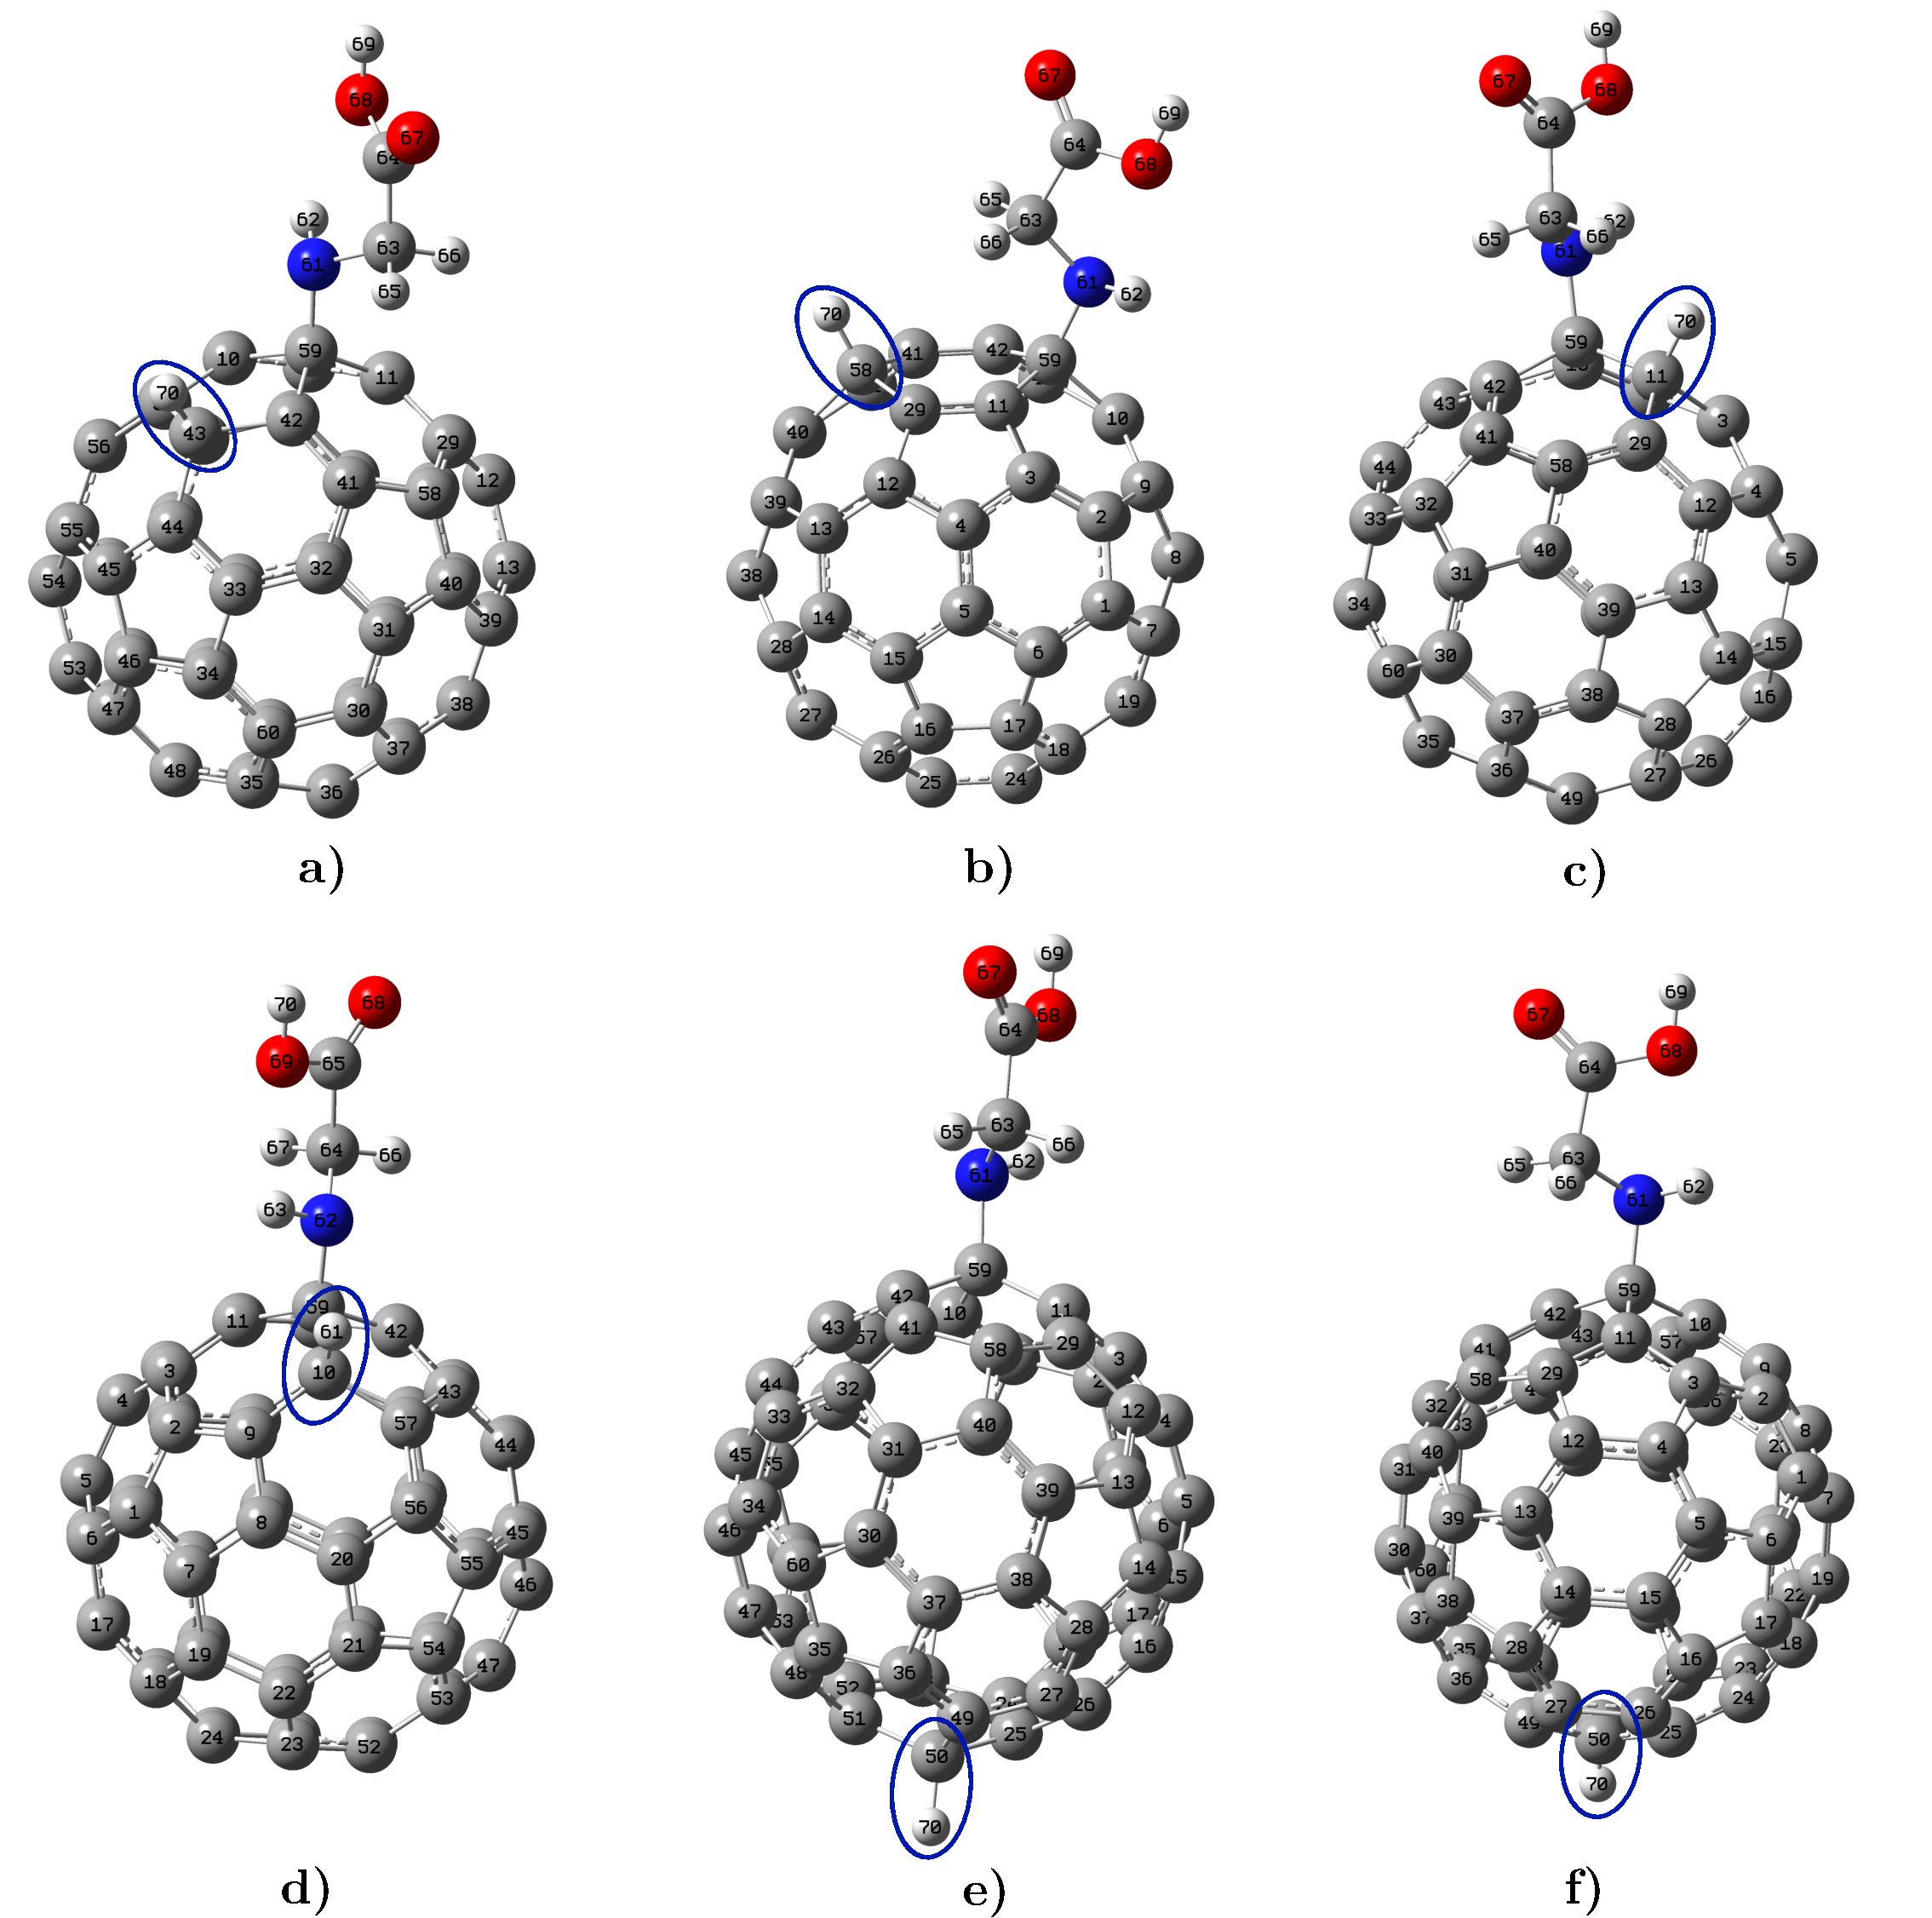
\includegraphics[width=1.0\textwidth]{imagenes/Resu/resu-1-opt.pdf}
      \caption{Isómeros propuestos para la primera adición de glicina al $C_{60}$. La glicina se une al carbono C59; los círculos azules señalan el segundo carbono del enlace evaluado: (a) C43, (b) C58, (c) C11, (d) C10, (e) C50 y (f) C51.}
      \label{fig:isomeros-gly1}
        \end{figure}
        
\begin{figure}[H]
      \centering
      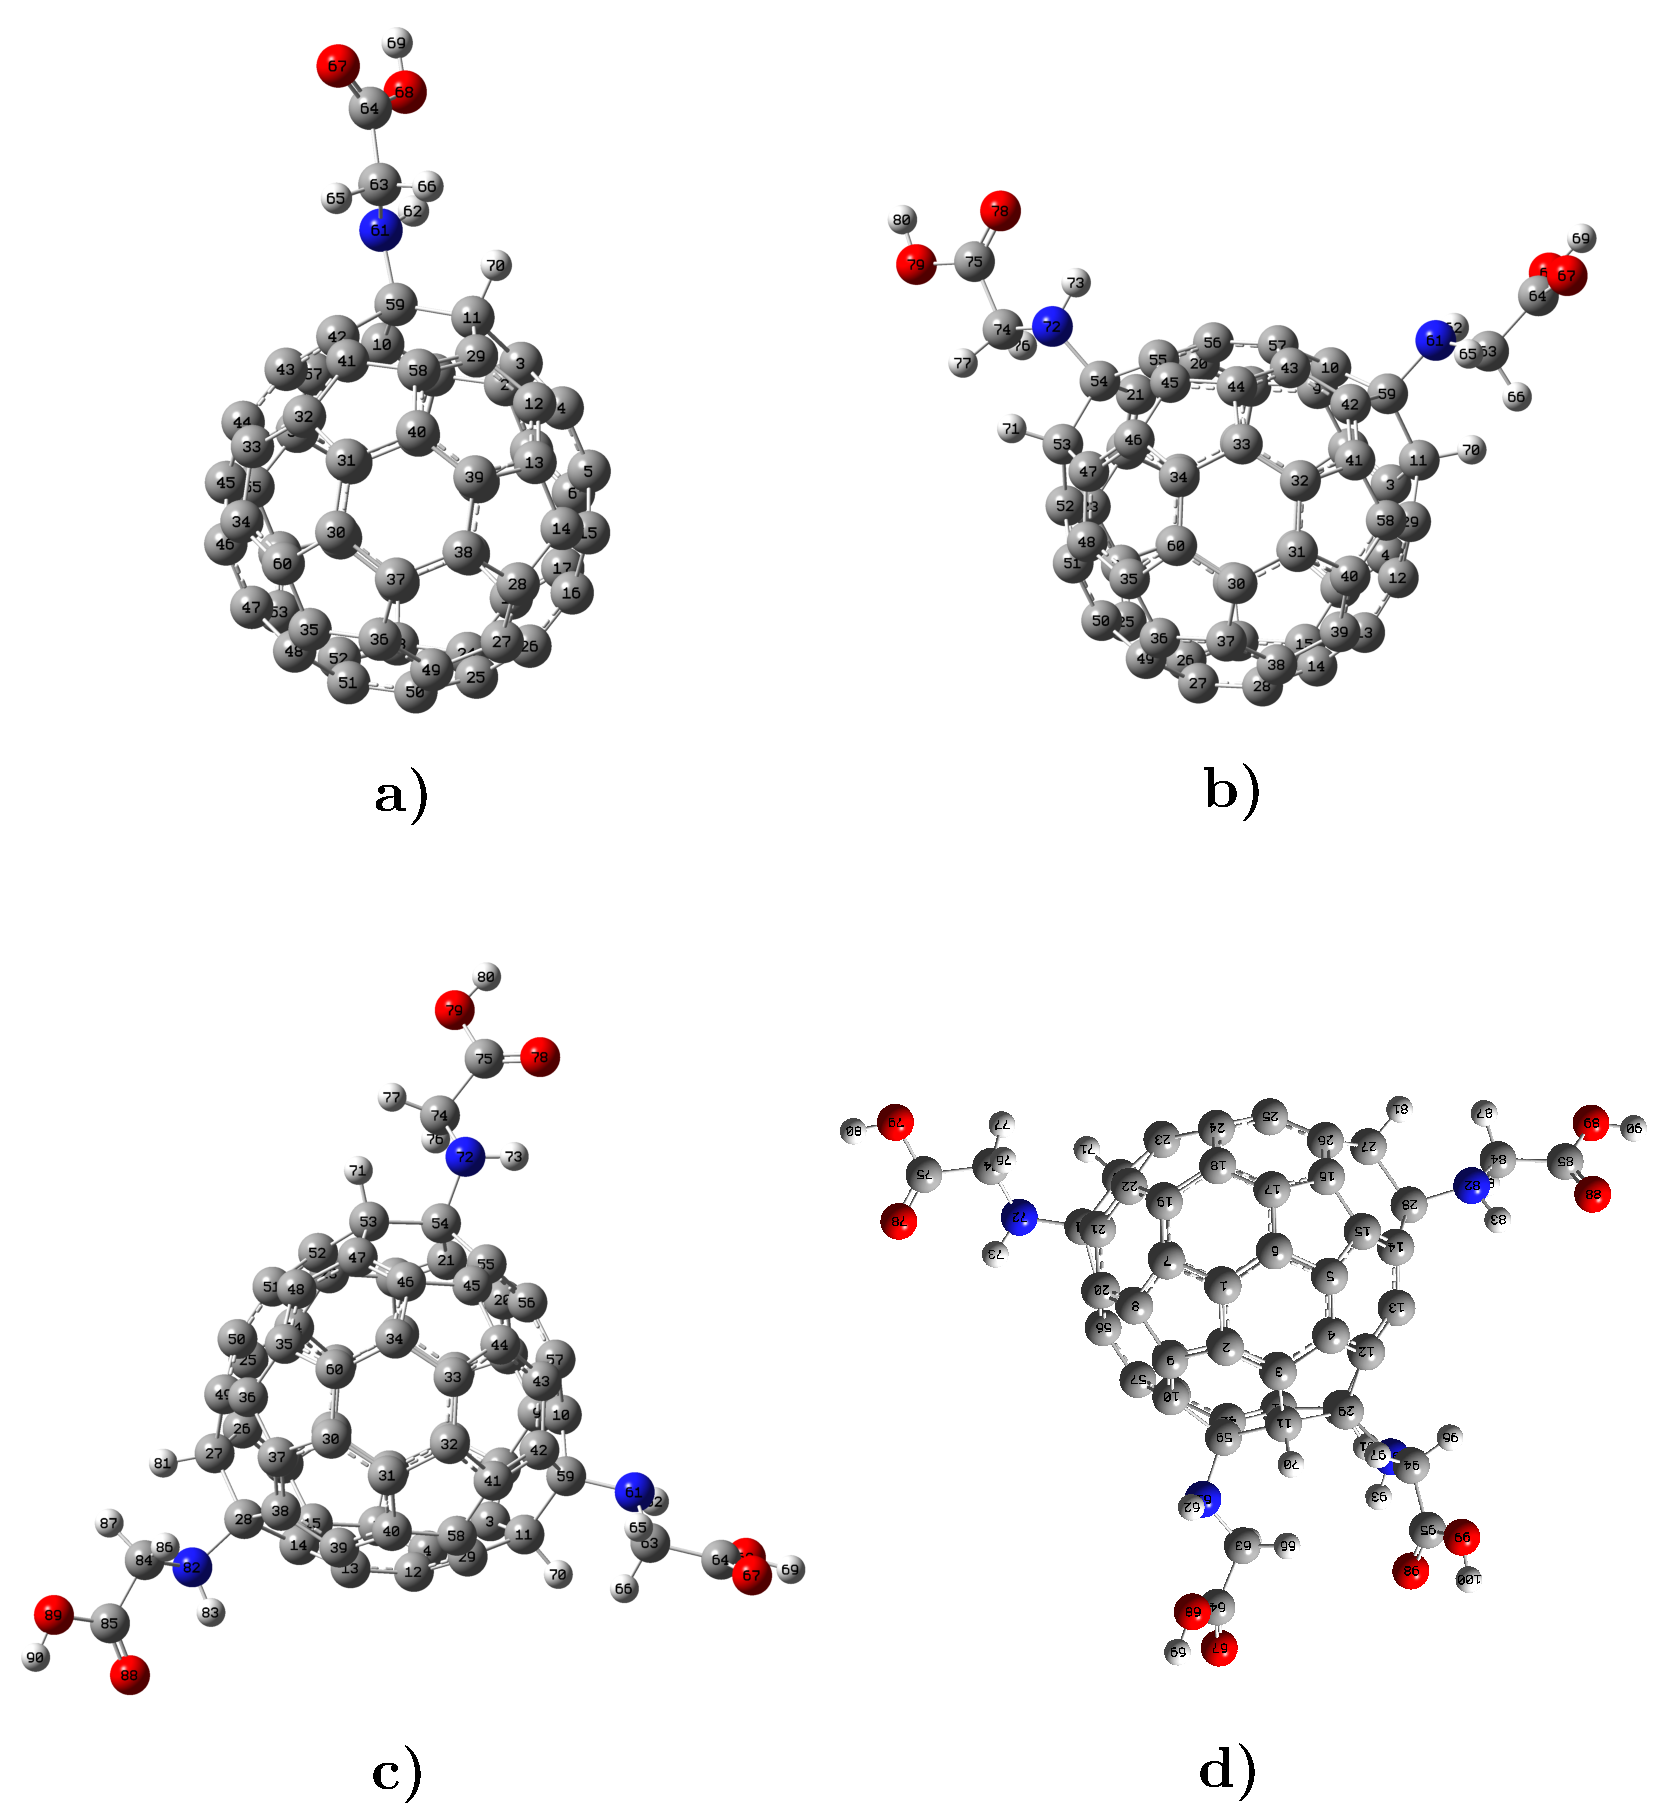
\includegraphics[width=1.0\textwidth]{imagenes/Resu/opt-gly-4.pdf}
      \caption{Estructuras optimizadas de los isómeros evaluados para la segunda adición de glicina al sistema  C\textsubscript{60}(Gly). Los paneles (a)--(d) corresponden a las alternativas estructurales comparadas en esta etapa.}
      \label{fig:isomeros-gly2}
        \end{figure}        

\begin{figure}[H]
      \centering
      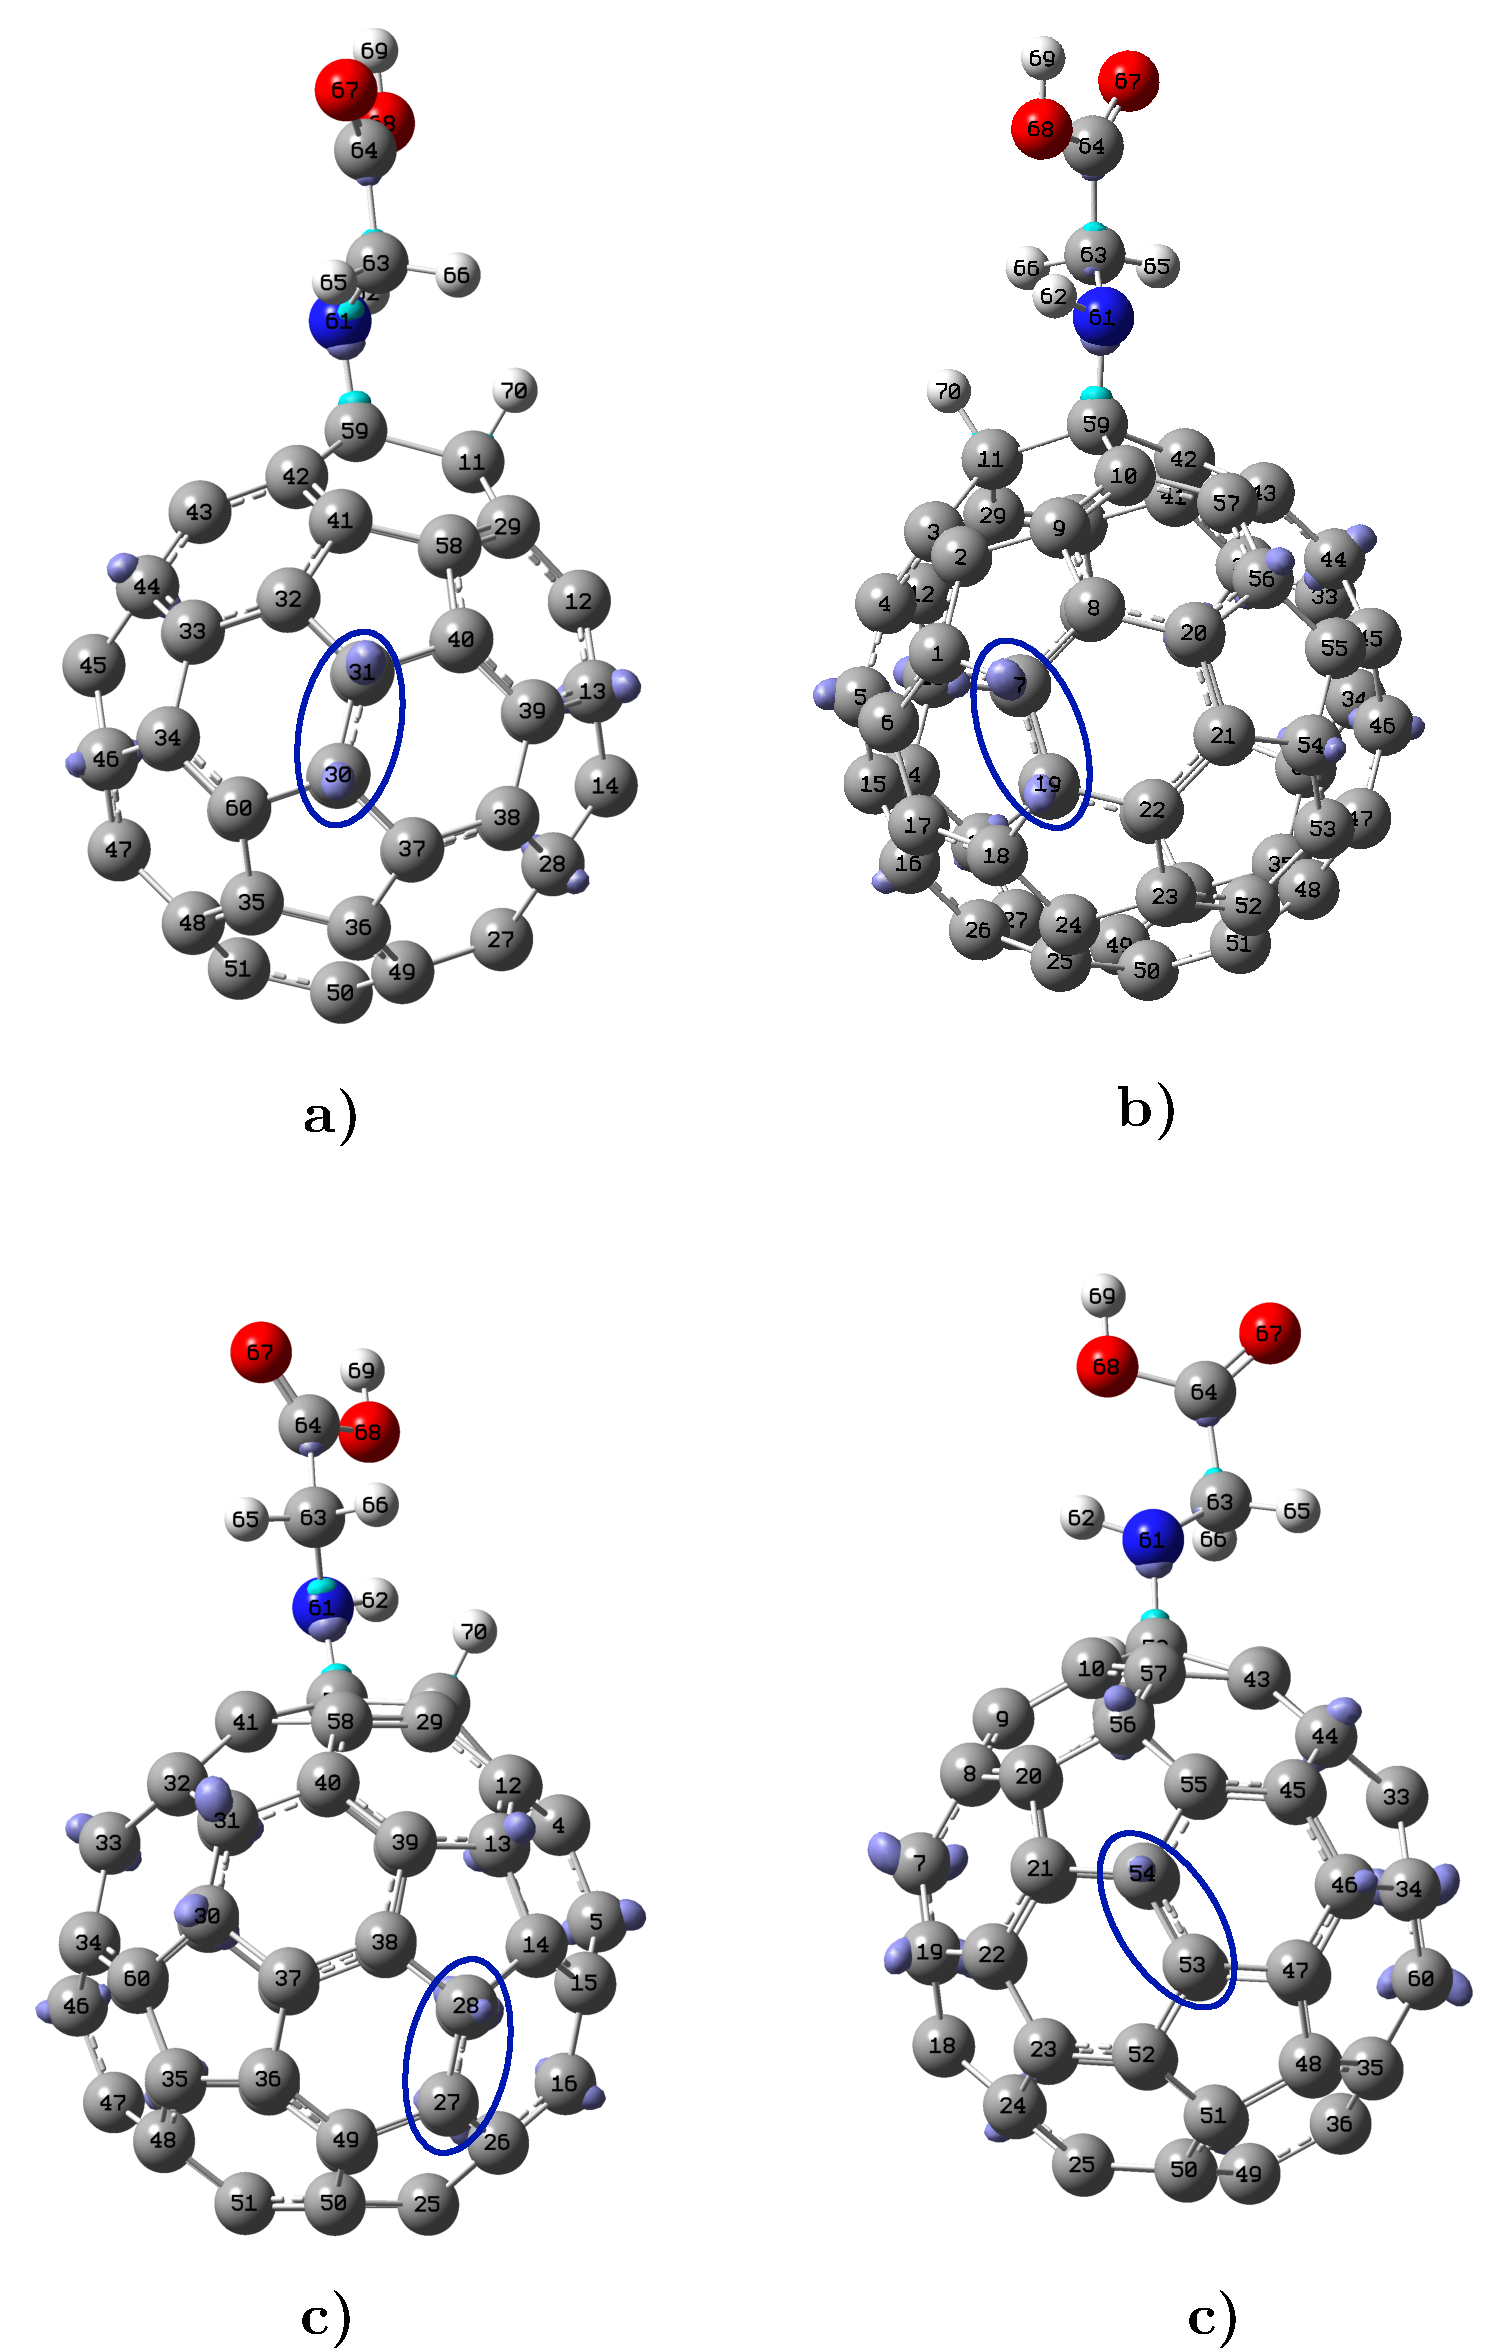
\includegraphics[width=0.7\textwidth]{imagenes/Resu/fukui-gly-resul-1.pdf}
      \caption{Estructuras seleccionadas durante la funcionalización secuencial de la jaula de $C_{60}$ con glicina. Los paneles muestran los sistemas con uno, dos, tres y cuatro grupos de glicina, respectivamente.}
      \label{fig:secuencia-gly}
        \end{figure}

\begin{figure}[H]
      \centering
      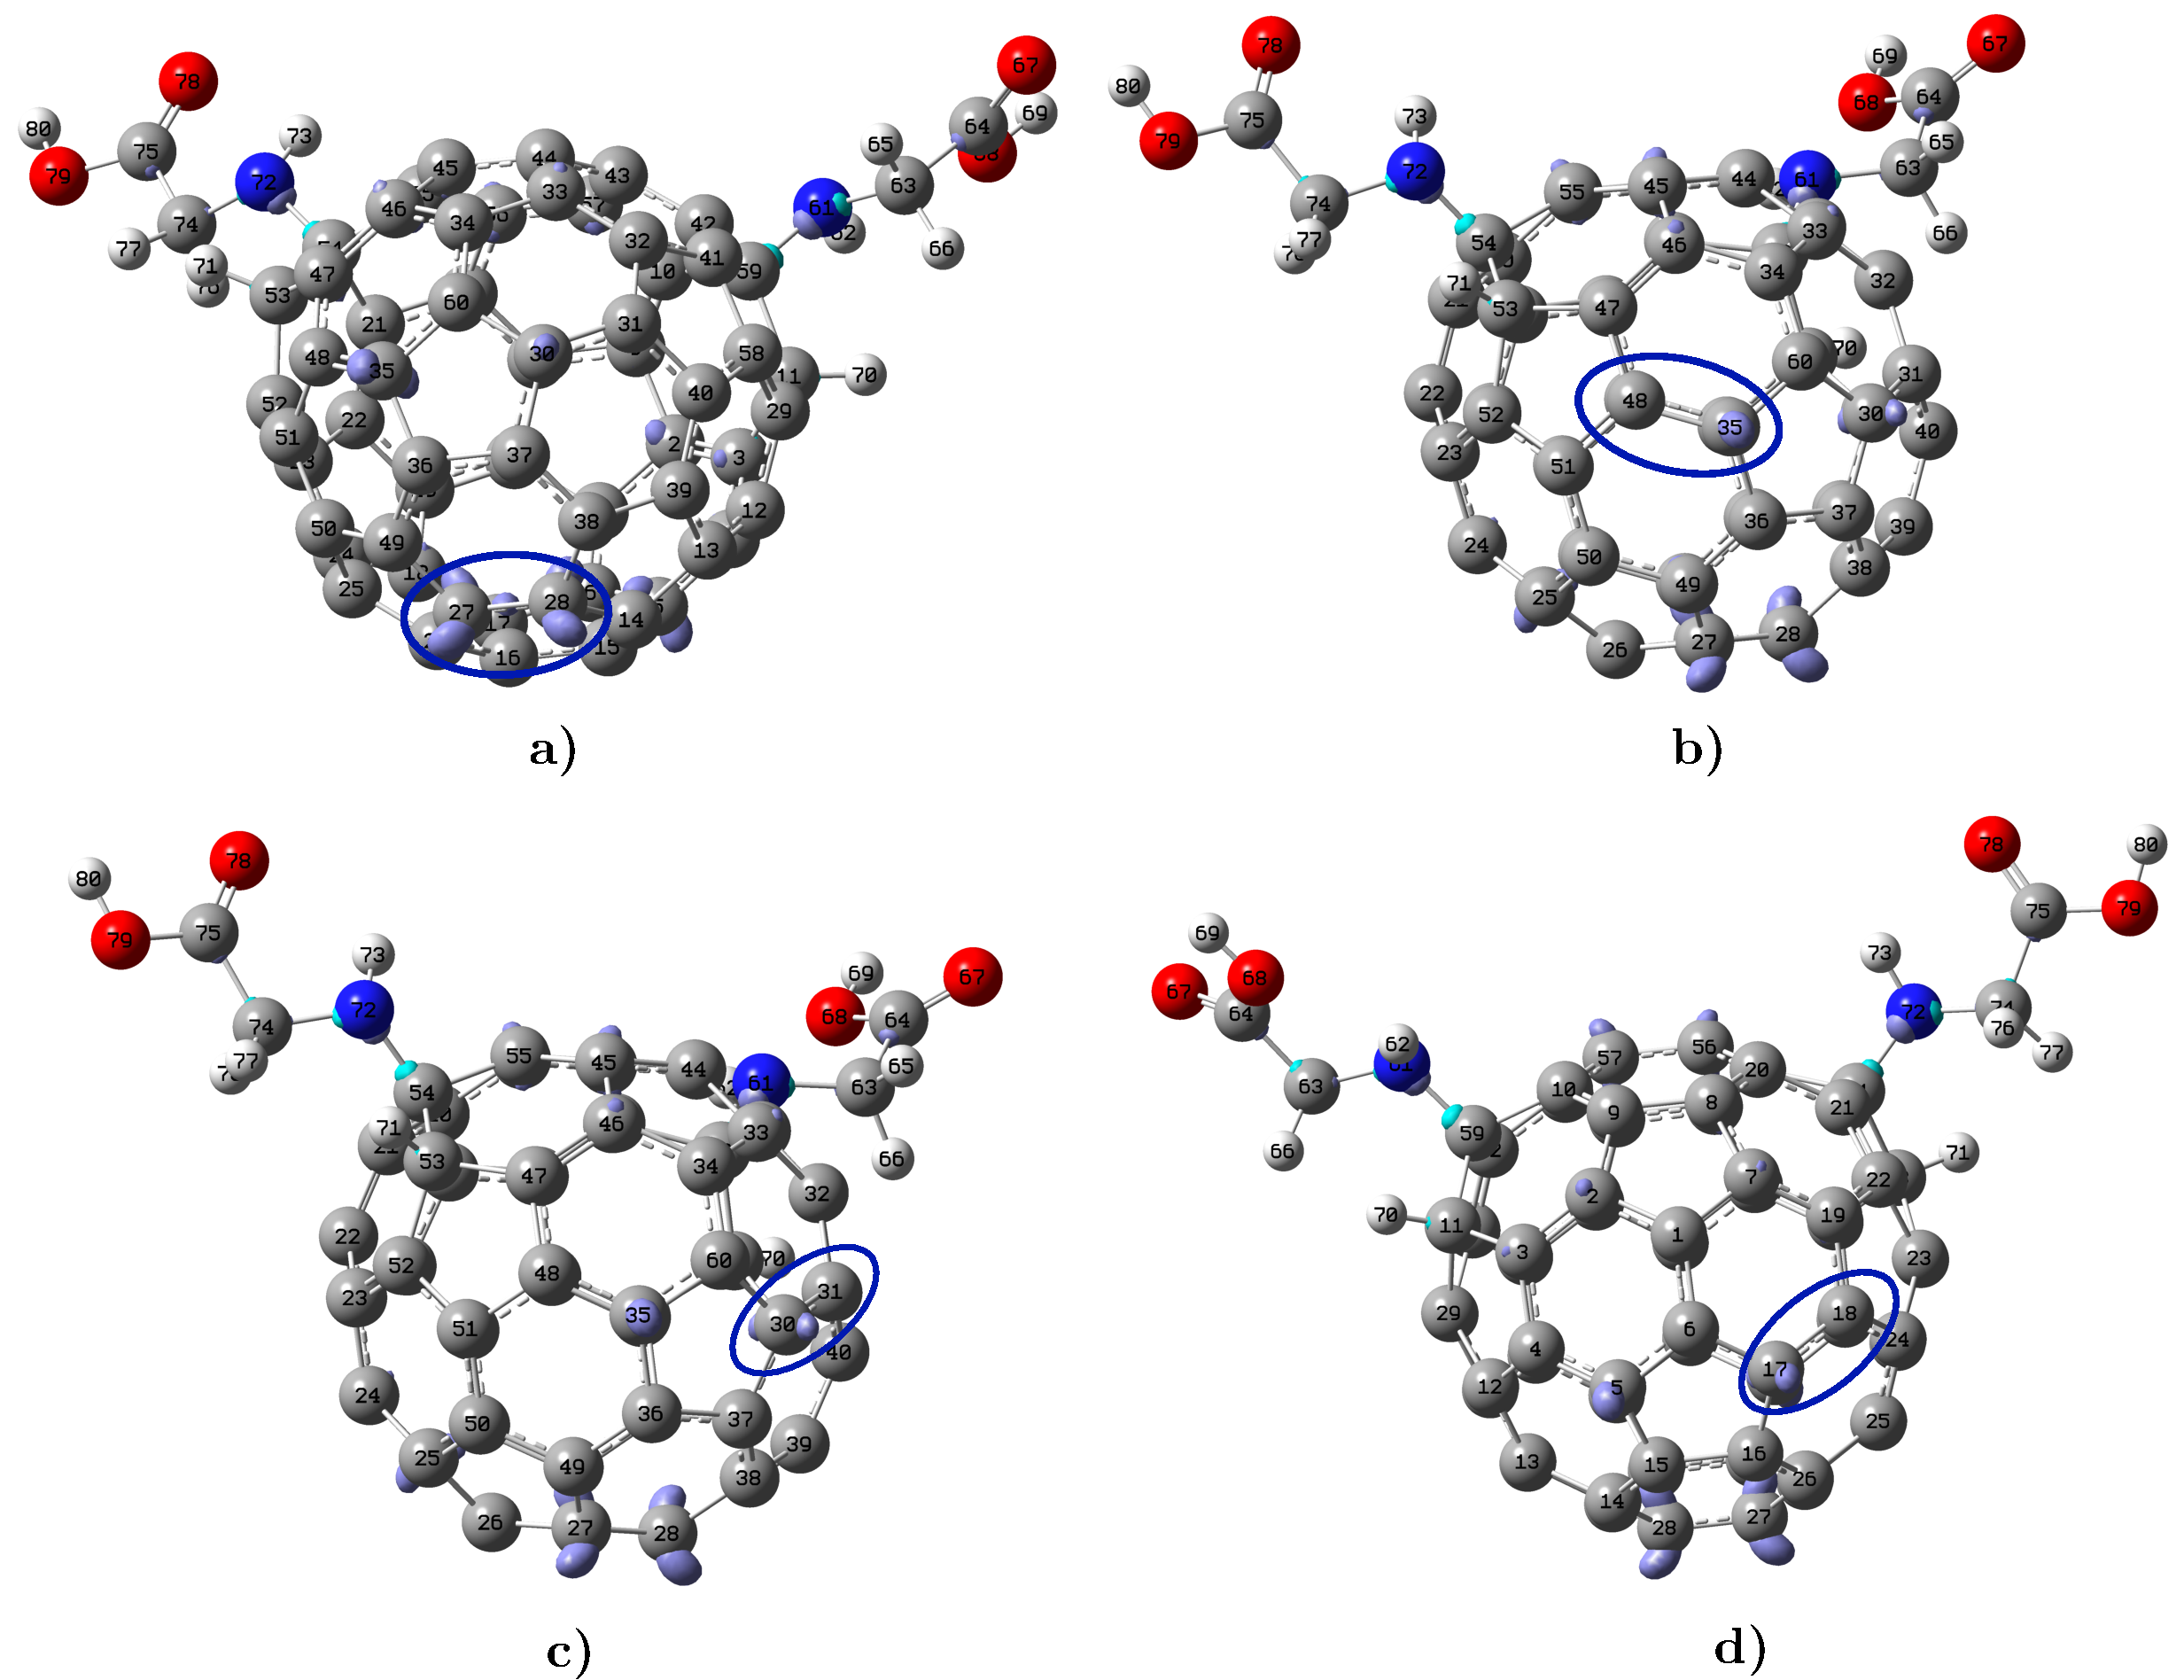
\includegraphics[width=1.0\textwidth]{imagenes/Resu/resu-2-fukui.pdf}
      \caption{Alternativas estructurales consideradas para continuar la funcionalización de $C_{60}$ con un tercer grupo de glicina. Los círculos azules indican los pares de carbonos evaluados como sitios de adición.}
      \label{fig:isomeros-gly3}
        \end{figure}

\begin{figure}[H]
      \centering
      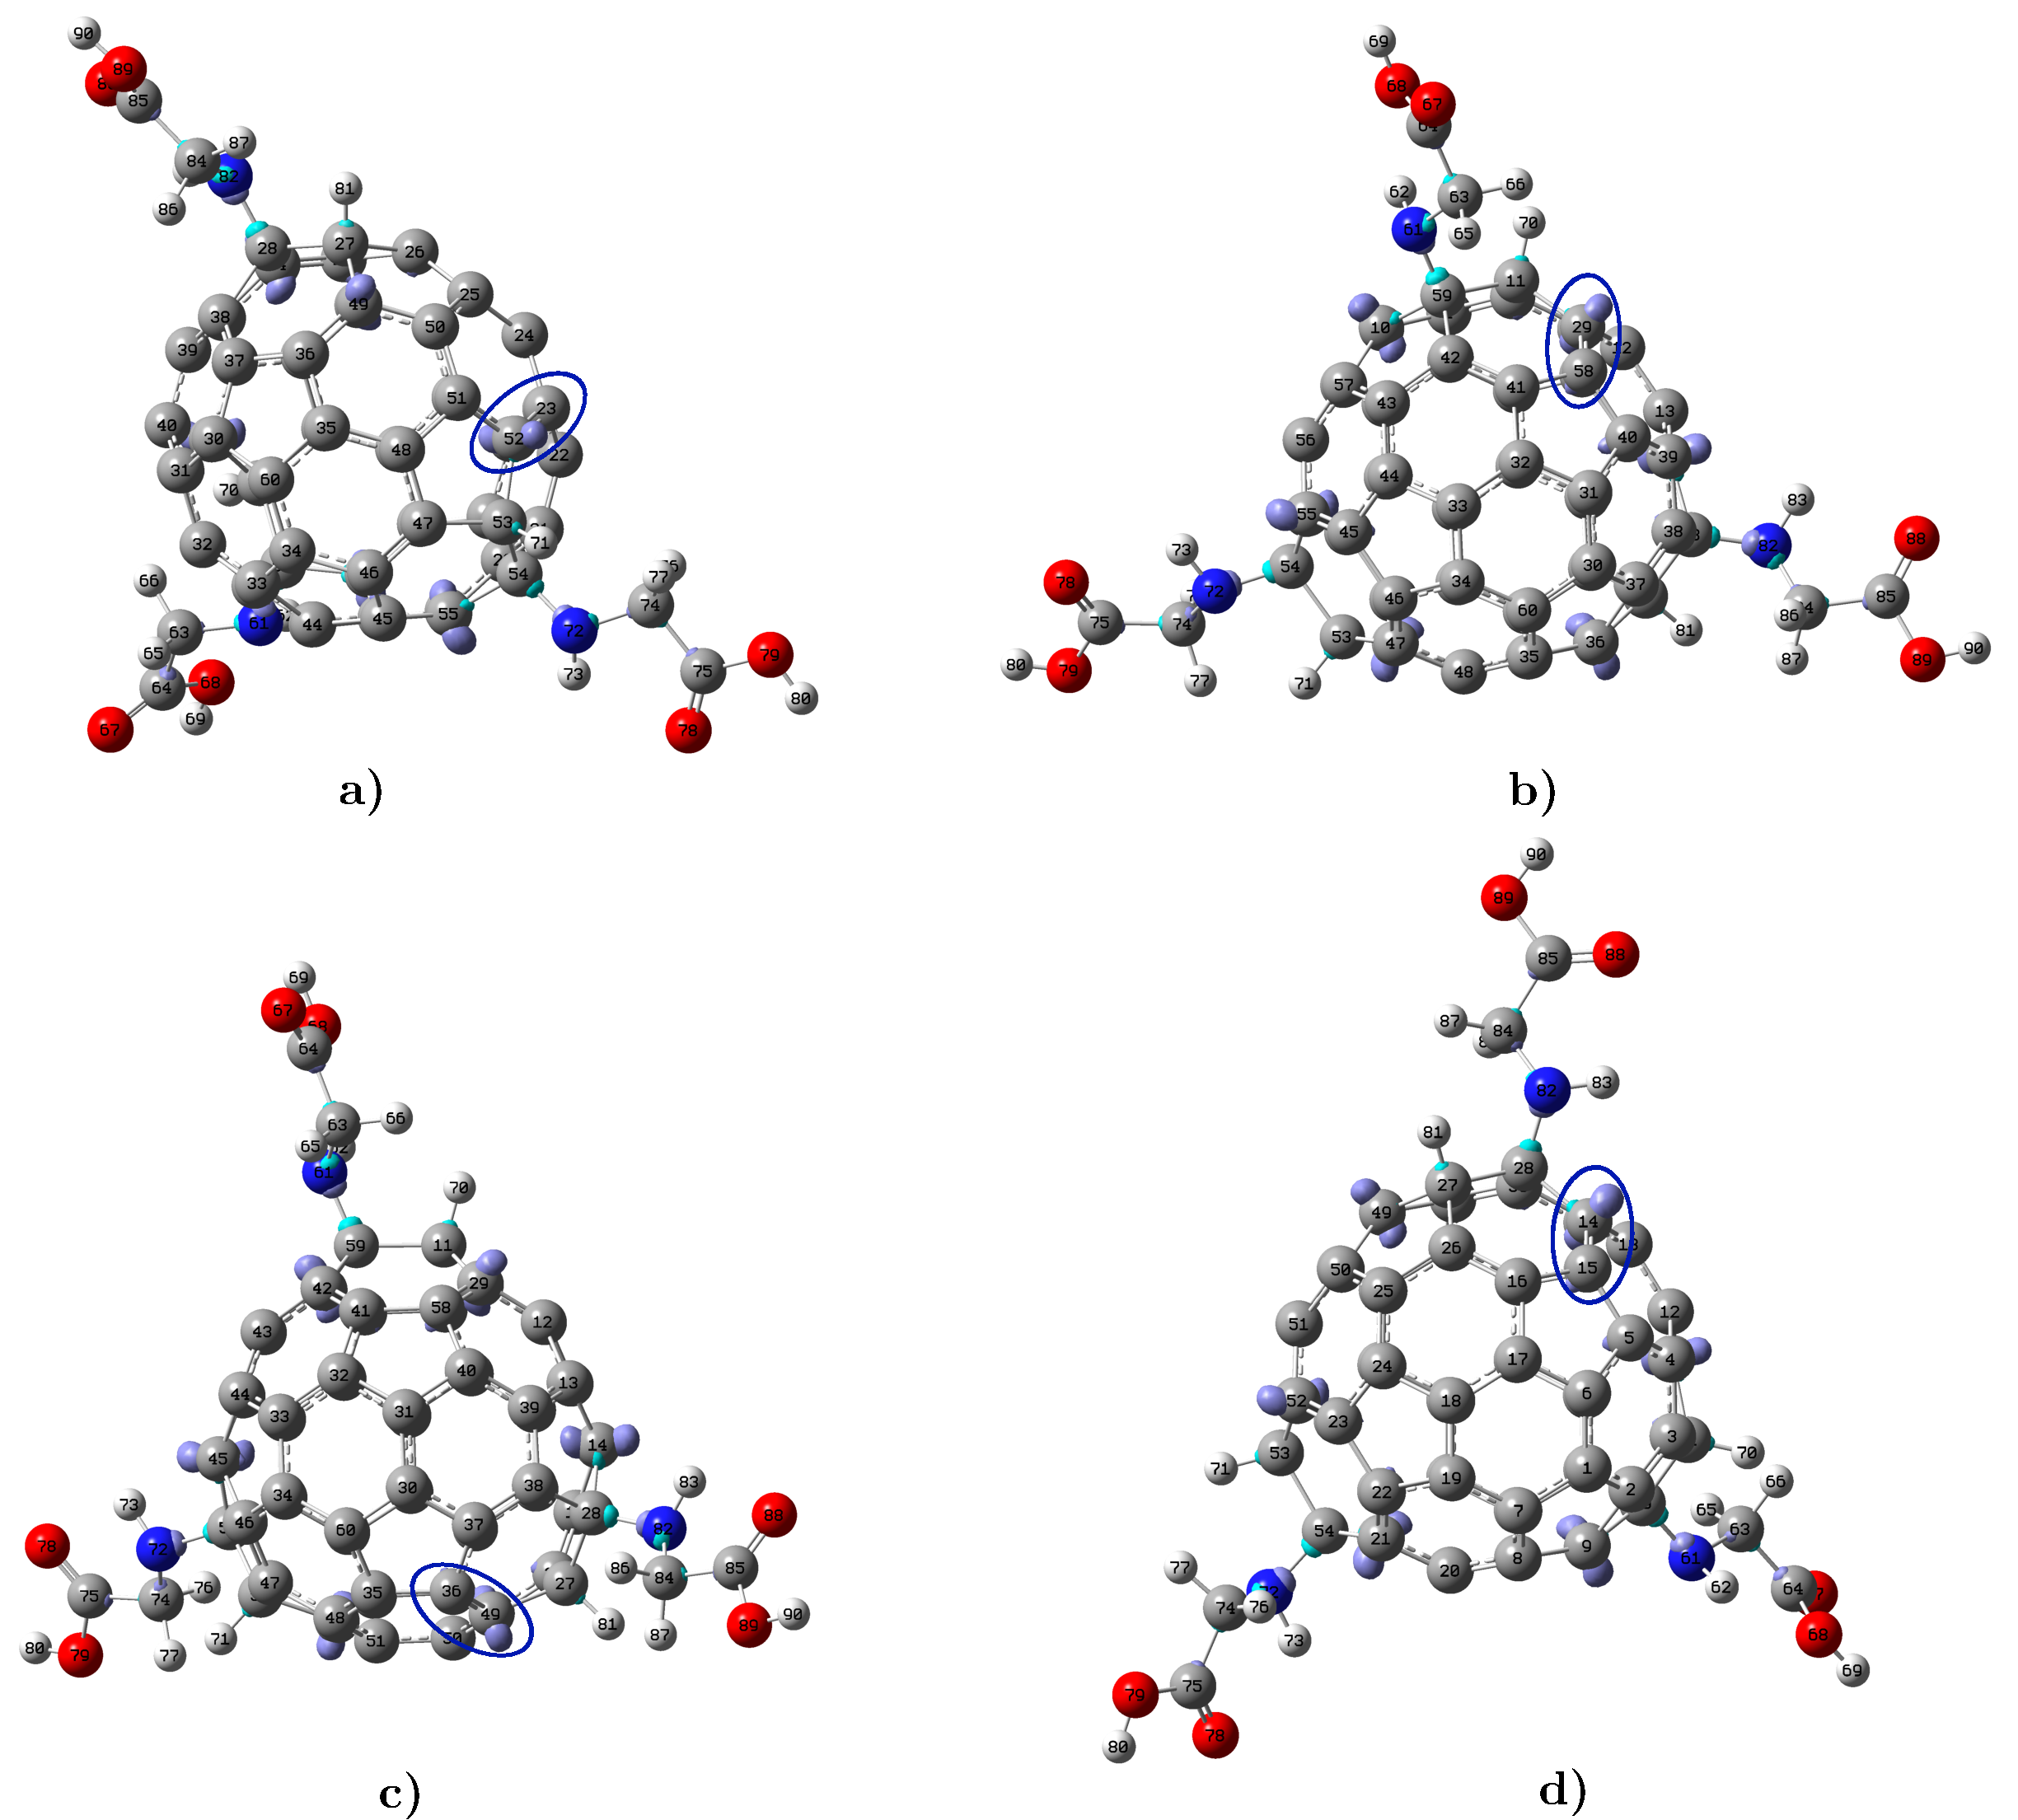
\includegraphics[width=1.0\textwidth]{imagenes/Resu/resu-3-fukui.pdf}
      \caption{Alternativas estructurales consideradas para la cuarta adición de glicina al sistema C\textsubscript{60}(Gly)\textsubscript{3}. Los círculos azules señalan los pares de carbonos analizados para formar el complejo C\textsubscript{60}(Gly)\textsubscript{4}.}
      \label{fig:isomeros-gly4}
        \end{figure}
    
    
 \section{Mecanismo de reacción y cálculo de los índices de reactividad local}

A partir de la optimización del primer aducto $C_{60}(\text{Gly})\text{-c}$, las adiciones sucesivas de las moléculas de glicina se fundamentaron en el análisis de los índices de reactividad local. Dado que la reacción transcurre mediante un mecanismo de adición nucleofílica donde el grupo amino de la glicina actúa como especie nucleófila y la jaula de $C_{60}$ como electrófilo, se calcularon las \textbf{funciones de Fukui para ataque nucleofílico ($f^+$)} sobre la superficie del sistema en cada etapa de funcionalización.

Las regiones de la jaula con mayor susceptibilidad reactiva se identificaron mediante la visualización de los lóbulos de densidad electrónica en las funciones de Fukui empleando un isovalor de $0.003\text{ a.u.}$ (Figuras~\ref{fig:secuencia-gly}, \ref{fig:secuencia-gly2}, \ref{fig:isomeros-gly3}) y \ref{fig:isomeros-gly4}). Los sitios de mayor reactividad se concentraron predominantemente sobre enlaces de tipo [6,6], los cuales conservan un mayor carácter de doble enlace y menor tensión de anillo. Las propuestas para las adiciones 2, 3 y 4 se establecieron estrictamente sobre las zonas donde los lóbulos mostraron las mayores magnitudes de reactividad local.

\section{Análisis de las adiciones secuenciales ($C_{60}(\text{Gly})_2$ a $C_{60}(\text{Gly})_4$)}

\paragraph{Segunda adición: $C_{60}(\text{Gly})_2$}
Para la formación del complejo difuncionalizado se evaluaron cuatro sitios candidatos propuestos a partir de los mapas de Fukui (Tabla~\ref{tab:adicion-secuencial-gly}). Como se observa en los resultados energéticos, la \textbf{Propuesta 4} (carbonos C54, C53) presentó la mayor estabilidad termodinámica, definíendose como la estructura de referencia ($0.000\text{ kcal mol}^{-1}$). Aunque las diferencias respecto a las demás alternativas no superan las $0.850\text{ kcal mol}^{-1}$ (candidatos 1, 2 y 3 con $0.696$, $0.789$ y $0.850\text{ kcal mol}^{-1}$, respectivamente), la ligera preferencia energética hacia la posición C54--C53 se atribuye a una menor repulsión estérica entre las cadenas de glicina y a una distribución electrónica de la red optimizada tras el primer ataque.

\paragraph{Tercera adición: $C_{60}(\text{Gly})_3$}
En la evaluación de la tercera molécula de glicina (Figura~\ref{fig:isomeros-gly3}), el mapa de reactividad de Fukui sobre $C_{60}(\text{Gly})_2$ identificó cuatro nuevas regiones objetivo. Entre ellas, la \textbf{Propuesta 1} (carbonos C28, C27) resultó ser el mínimo global con $0.000\text{ kcal mol}^{-1}$. A diferencia de la etapa anterior, en esta adición se observa una clara diferenciación energética: la Propuesta 2 (C35, C48) se encuentra fuertemente desestabilizada a $+3.935\text{ kcal mol}^{-1}$, mientras que las Propuestas 3 (C30, C31) y 4 (C17, C18) se ubican a $+1.142$ y $+1.208\text{ kcal mol}^{-1}$, respectivamente. Este incremento en la barrera termodinámica evidencia que la acumulación de tres grupos voluminosos sobre la jaula comienza a generar un impedimento estérico significativo y una pertubación considerable sobre la conjugación $\pi$ cíclica.

\paragraph{Cuarta adición: $C_{60}(\text{Gly})_4$}
Finalmente, para la tetrafuncionalización (Figura~\ref{fig:isomeros-gly4}), el análisis de reactividad sobre $C_{60}(\text{Gly})_3$ permitió formular cuatro propuestas finales. La \textbf{Propuesta 2} (carbonos C29, C58) mostró la mayor estabilidad termodinámica ($0.000\text{ kcal mol}^{-1}$), seguida de cerca por la Propuesta 3 (C49, C36 a $+0.640\text{ kcal mol}^{-1}$) y la Propuesta 1 (C52, C23 a $+0.676\text{ kcal mol}^{-1}$), mientras que la Propuesta 4 (C14, C15) resultó ser la menos favorable ($+2.180\text{ kcal mol}^{-1}$). 

La estrecha cercanía energética entre las tres primeras propuestas ($< 0.7\text{ kcal mol}^{-1}$) ocurre debido a que corresponden a enlaces [6,6] topológicamente equivalentes dentro de los dominios no funcionalizados de la jaula. Sin embargo, la ventaja energética sutil de la Propuesta 2 (C29, C58) está dictada por las interacciones intramoleculares secundarias, tales como el posible ordenamiento de los protones libres. Estas interacciones modulan la reactividad local de Fukui y determinan la configuración de mayor estabilidad para el sistema final $C_{60}(\text{Gly})_4$ Figura~\ref{fig:isomeros-gly4}.  
\section{Análisis de descriptores de reactividad global PI y AE)}
\begin{table}[H]
    \centering
    \caption{Energías totales calculadas en kcal/mol para la glicina, el fullereno $C_{60}$ y el sistema funcionalizado  C\textsubscript{60}(Gly).}
    \label{tab:energias-referencia}
    \renewcommand{\arraystretch}{1.15}
    \begin{tabular}{lccc}
        \toprule
        \textbf{Sistema} & \textbf{PI (eV)} & \textbf{AE (eV)}\\
        \midrule
         C\textsubscript{60}(Gly)\textsubscript{4} & 6.849
 & 1.779 \\
        Fullereno  C\textsubscript{60} & 7.608
 & 2.454 \\
        \bottomrule
    \end{tabular}
\end{table}
{Análisis de parámetros de reactividad global y potencial biológico}

El análisis de los parámetros reactivos globales presentados en la Tabla~\ref{tab:energias-referencia} revela modificaciones sustanciales en las propiedades electrónicas del fulereno tras la tetrafuncionalización con glicina. Se observa una reducción significativa en el Potencial de Ionización ($PI$), pasando de $7.608\text{ eV}$ en el $C_{60}$ prístino a $6.849\text{ eV}$ en el complejo $C_{60}(\text{Gly})_4$. Un valor menor de $PI$ indica que la energía del orbital molecular ocupado de mayor energía (HOMO) se ha elevado, disminuyendo la barrera energética requerida para la extracción de un electrón. Esta mayor facilidad para la donación electrónica posiciona al sistema $C_{60}(\text{Gly})_4$ como un potente agente reductor y antioxidante, capaz de neutralizar Especies Reactivas de Oxígeno (ROS) en entornos celulares mediante mecanismos de transferencia de un electrón (SET).

Por otro lado, la Afinidad Electrónica ($AE$) experimentó una disminución desde $2.454\text{ eV}$ en la jaula prístina hasta $1.779\text{ eV}$ en el aducto $C_{60}(\text{Gly})_4$. Mientras que el $C_{60}$ sin funcionalizar actúa primordialmente como un aceptor de electrones altamente eficiente debido a su elevada $AE$, la adición de los cuatro residuos de glicina modula el carácter amfotérico de la jaula, atenuando la capacidad electroatractora e incrementando fuertemente el perfil electrodonador.

En conjunto, la funcionalización secuencial con glicina cumple un doble propósito de alto valor biomédico: por un lado, incrementa la capacidad antioxidante del sistema al reducir el $PI$; por otro, introduce grupos funcionales polares ($-\text{COOH}$ y $-\text{NH}_2$) que le confieren solubilidad en medios acuosos y biocompatibilidad, superando la principal limitación de insolubilidad del $C_{60}$ prístino en medios fisiológicos.


    
    \section{Potencial electrostático superficial}
     \begin{table}[H]
    \centering
    \caption{Valores de potencial electrostático para cada sistema de C\textsubscript{60}(Gly).}
    \label{tab:potencial-electrostatico}
    \renewcommand{\arraystretch}{1.15}
    \begin{tabular}{lc}
        \toprule
        \textbf{Sistema} & \textbf{Valor de potencial electrostático} \\
        \midrule
        Fullereno C\textsubscript{60}(Gly) & 1.465 \\
       C\textsubscript{60}(Gly) & 0.975 \\
        C\textsubscript{60}(Gly)\textsubscript{2} & 2.289 \\
        C\textsubscript{60}(Gly)\textsubscript{3} & 2.556 \\
        C\textsubscript{60}(Gly)\textsubscript{4} & 6.024 \\
        \midrule
        \textbf{Promedio} & \textbf{2.662} \\
        \bottomrule
        \end{tabular}
\end{table}

El análisis del Potencial Electrostático Superficial (MEP) presentado en la Tabla~\ref{tab:potencial-electrostatico} revela una clara tendencia hacia la electropositividad a medida que avanza la funcionalización secuencial del $C_{60}$. En el aducto monofuncionalizado $C_{60}(\text{Gly})$, el potencial promedio se sitúa en $0.975\text{ kcal mol}^{-1}$; sin embargo, la incorporación progresiva de residuos de aminoácido provoca un incremento sustancial hasta alcanzar un valor máximo de $6.024\text{ kcal mol}^{-1}$ en el complejo tetrafuncionalizado $C_{60}(\text{Gly})_4$. 

Este marcado desplazamiento hacia un perfil predominantemente electropositivo en el $C_{60}(\text{Gly})_4$ —el cual supera en más de cuatro veces al valor del $C_{60}$ prístino ($1.466\text{ kcal mol}^{-1}$)— se explica por la acumulación neta de protones ($H$) pertenecientes a los grupos $-\text{NH}_2$ y $-\text{COOH}$. Como se observa en el análisis atómico de la Figura~\ref{fig:esp-promedio}, la densidad electropositiva individual de los protones (con picos que superan los $+30\text{ kcal mol}^{-1}$) termina por dominar el promedio global del sistema sobre los aportes electronegativos de los átomos de oxígeno y nitrógeno (localizados en torno a $-20\text{ kcal mol}^{-1}$).

\subsection{Implicaciones en el reconocimiento molecular con la proteína 2FOM (DENV2)}

Desde la perspectiva del reconocimiento molecular, el elevado carácter electropositivo global alcanzado en el sistema $C_{60}(\text{Gly})_4$ constituye un factor determinante para sus aplicaciones biológicas. Específicamente, en la proteína de envoltura del virus del Dengue serotipo 2 (DENV2, PDB ID: 2FOM), la arquitectura del sitio activo y de diversas cavidades de superficie cuenta con una alta densidad de aminoácidos aniónicos (tales como ácido aspártico y ácido glutámico), los cuales generan campos de potencial electrostático fuertemente negativos.

Por consiguiente, el incremento en la electropositividad del derivado tetrafuncionalizado actúa como un potente impulsor termodinámico, favoreciendo una atracción electrostática de largo alcance hacia estas cavidades aniónicas de la proteína 2FOM. Al mismo tiempo, la presencia de polos electronegativos locales en los oxígenos/nitrógenos y las regiones neutras sobre la jaula de $C_{60}$ (visibles en el mapa tridimensional de la Figura~\ref{fig:mep-gly4}) le otorgan al ligando la versatilidad necesaria para establecer puentes de hidrógeno secundarios y contactos hidrofóbicos, garantizando un acoplamiento molecular estable y específico en el dominio biológico evaluado.


Los valores de la Tabla~\ref{tab:potencial-electrostatico} muestran que la funcionalización con glicina modifica el potencial electrostático promedio del sistema. El fullereno presenta un valor de 1.466, mientras que la primera adición de glicina reduce este valor a 0.975. A partir de la segunda adición, el potencial aumenta a 2.289 y 2.556 para los sistemas con dos y tres glicinas, respectivamente, hasta alcanzar 6.024 en C\textsubscript{60}(Gly)\textsubscript{4}. Por lo tanto, el cambio no es lineal en la primera etapa, pero la tendencia general a partir de la segunda incorporación indica que los grupos de glicina afectan de manera importante la distribución electrónica de la superficie molecular.

La Figura~\ref{fig:esp-promedio} permite observar esta variación a nivel de los sitios evaluados. La coexistencia de valores positivos y negativos indica que la superficie del sistema no es uniforme y que conserva regiones con distinto carácter electrostático. Conforme aumenta el número de grupos de glicina, estas regiones se redistribuyen alrededor de la jaula de C\textsubscript{60}(Gly), lo cual es consistente con la incorporación de grupos funcionales polares. El mapa de potencial electrostático de la Figura~\ref{fig:mep-gly4} complementa este resultado al mostrar que, en el sistema con cuatro glicinas, las zonas de mayor variación se localizan principalmente alrededor de los sustituyentes.
    
    \begin{figure}[H]
      \centering
      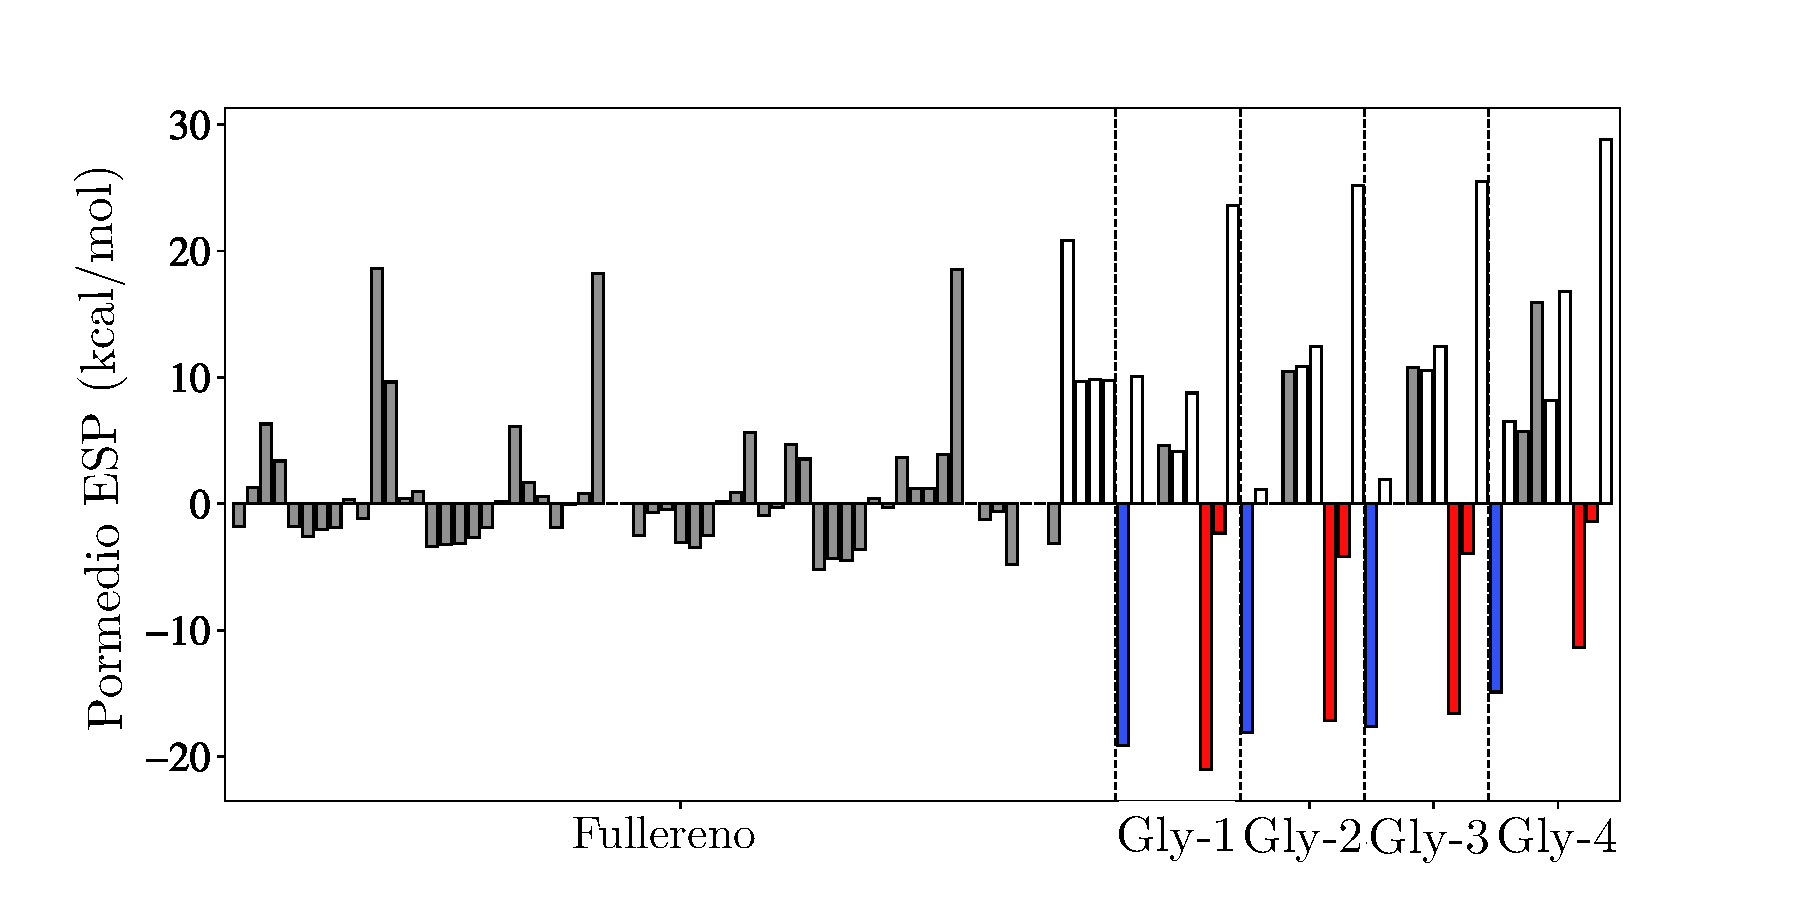
\includegraphics[width=1.0\textwidth]{imagenes/Resu/figure_2.pdf}
      \caption{Distribución de los valores de potencial electrostático promedio para el fullereno y los sistemas funcionalizados con una a cuatro glicinas. Las líneas verticales discontinuas separan cada sistema analizado.}
      \label{fig:esp-promedio}
        \end{figure}
    
    
    
                      
\begin{figure}[H]
      \centering
      \includegraphics[width=1.0\textwidth]{imagenes/Resu/figure_5.png}
      \caption{Mapa de potencial electrostático molecular del complejo C\textsubscript{60}(Gly)\textsubscript{4} observado desde dos orientaciones. La figura muestra la heterogeneidad de la superficie electrónica alrededor de la jaula de fullereno y de los grupos de glicina.}
      \label{fig:mep-gly4}
        \end{figure}
        
        
 \section{Distribución del potencial electrostático molecular (MEP)}

En la Figura~\ref{fig:esp-promedio} se presenta la distribución puntual del promedio del Potencial Electrostático (ESP, expresado en $\text{kcal mol}^{-1}$) para cada átomo del sistema, determinado mediante el software Multiwfn. 

En la jaula del fullereno prístino, los átomos de carbono muestran valores de potencial muy cercanos a cero (oscilando ligeramente en una franja neutra), lo que refleja la simetría electrónica y el carácter apolar de la red conjugada $\pi$. Sin embargo, al evaluar las adiciones secuenciales de glicina (sistemas Gly-1 a Gly-4), se evidencia una clara polarización electrónica espacial:
\begin{enumerate}
    \item \textbf{Átomos electronegativos ($O$ y $N$):} Los átomos de oxígeno y nitrógeno de los residuos de glicina presentan los potenciales más negativos del sistema, alcanzando valores mínimos de hasta $-20\text{ kcal mol}^{-1}$ (barras rojas y azules orientadas hacia abajo en la Figura~\ref{fig:esp-promedio}).
    \item \textbf{Átomos de hidrógeno polar ($H$):} Los protones pertenecientes a los grupos funcionales de la glicina exhiben los potenciales más electropositivos, superando los $+20$ y $+30\text{ kcal mol}^{-1}$ (barras dirigidas hacia arriba).
    \item \textbf{Carbonos de la jaula y grupos adyacentes:} Presentan una modulación sutil dependiendo de su cercanía a los grupos funcionales, manteniendo los carbonos de las glicinas un carácter moderadamente positivo.
\end{enumerate}

Por su parte, la Figura~\ref{fig:mep-gly4} ilustra la topografía del Mapa de Potencial Electrostático Molecular (MEP) para el complejo $C_{60}(\text{Gly})_4$ desde dos orientaciones (frente y vuelta), corroborando tridimensionalmente la heterogeneidad cuantitativa observada en la Figura~\ref{fig:esp-promedio}. La superficie molecular exhibe una marcada anfipaticidad:
\begin{itemize}
    \item \textbf{Regiones rojas (Potencial electronegativo):} Concentradas sobre los átomos de oxígeno de los carboxilos y nitrógenos, constituyendo sitios idóneos para actuar como aceptores de puentes de hidrógeno o interactuar con residuos catiónicos.
    \item \textbf{Regiones azules intensas (Potencial electropositivo):} Localizadas sobre los protones de los grupos funcionales, actuando como donadores de puentes de hidrógeno y sitios de atracción electrostática hacia residuos aniónicos.
    \item \textbf{Regiones verdes (Potencial neutro/apolar):} La superficie de la jaula de $C_{60}$ conserva una coloración verdosa dominante (potencial cercano a $0\text{ kcal mol}^{-1}$), demostrando que el núcleo no pierde su capacidad de establecer interacciones hidrofóbicas.
\end{itemize}

\subsection{Implicaciones en el reconocimiento molecular con la proteína 2FOM (DENV2)}

Esta distribución electrostática heterogénea demuestra que el aducto $C_{60}(\text{Gly})_4$ actúa como un ligando multifuncional con alta versatilidad de acoplamiento. A diferencia del fullereno prístino —cuyo mecanismo de interacción está restringido únicamente a contactos hidrofóbicos—, la tetrafuncionalización le confiere al sistema la capacidad de establecer tres tipos fundamentales de interacciones en el sitio de reconocimiento de la proteína de envoltura del virus del Dengue (DENV2, PDB ID: 2FOM):
\begin{enumerate}
    \item \textbf{Interacciones electrostáticas catiónicas:} Los lóbulos electropositivos (azules, $+30\text{ kcal mol}^{-1}$) se acoplan preferentemente con cavidades aniónicas ricas en residuos de ácido aspártico (Asp) y ácido glutámico (Glu).
    \item \textbf{Interacciones electrostáticas aniónicas:} Los lóbulos electronegativos (rojos, $-20\text{ kcal mol}^{-1}$) interactúan de manera complementaria con residuos cargados positivamente, tales como lisina (Lys), arginina (Arg) o histidina (His).
    \item \textbf{Interacciones de van der Waals y apolares:} La superficie verde neutra de la jaula permite el empaquetamiento hidrofóbico con aminoácidos aromáticos y alifáticos (como leucina, isoleucina, fenilalanina y triptófano) dentro del bolsillo catalítico o de unión de la proteína 2FOM.
\end{enumerate}

En conclusión, la funcionalización con glicina no solo mejora la solubilidad del nanomaterial, sino que genera una superficie electrónica multipolar altamente adaptable a la diversidad de aminoácidos presentes en la diana biológica 2FOM.       
        
        
        
        
        
        
        
                
\section{Acoplamiento molecular}  
La proteasa NS2B/NS3 del serotipo 2 del virus del dengue (DENV-2), con una masa molecular de $26.57\ \text{kDa}$, representa un blanco terapéutico primordial por su papel clave en la replicación viral. Al evaluar el modelo en conformación abierta e inactiva (PDB ID: \textbf{2FOM}) reconstruido en sus regiones desordenadas mediante AlphaFold, se observa que la estructura presenta una alta fidelidad conformacional.

En el mapa de Ramachandran se aprecia una distribución óptima de los ángulos diedros ($\phi, \psi$), donde la gran mayoría de los residuos se ubican en zonas energéticamente favorecidas. A partir de esta base estructural, los $100\ \text{ns}$ de dinámica molecular (MD) bajo el campo de fuerzas CHARMM36 reflejan la respuesta conformacional y la estabilidad del sistema en solución acuosa.

\begin{figure}[H]
    \centering
    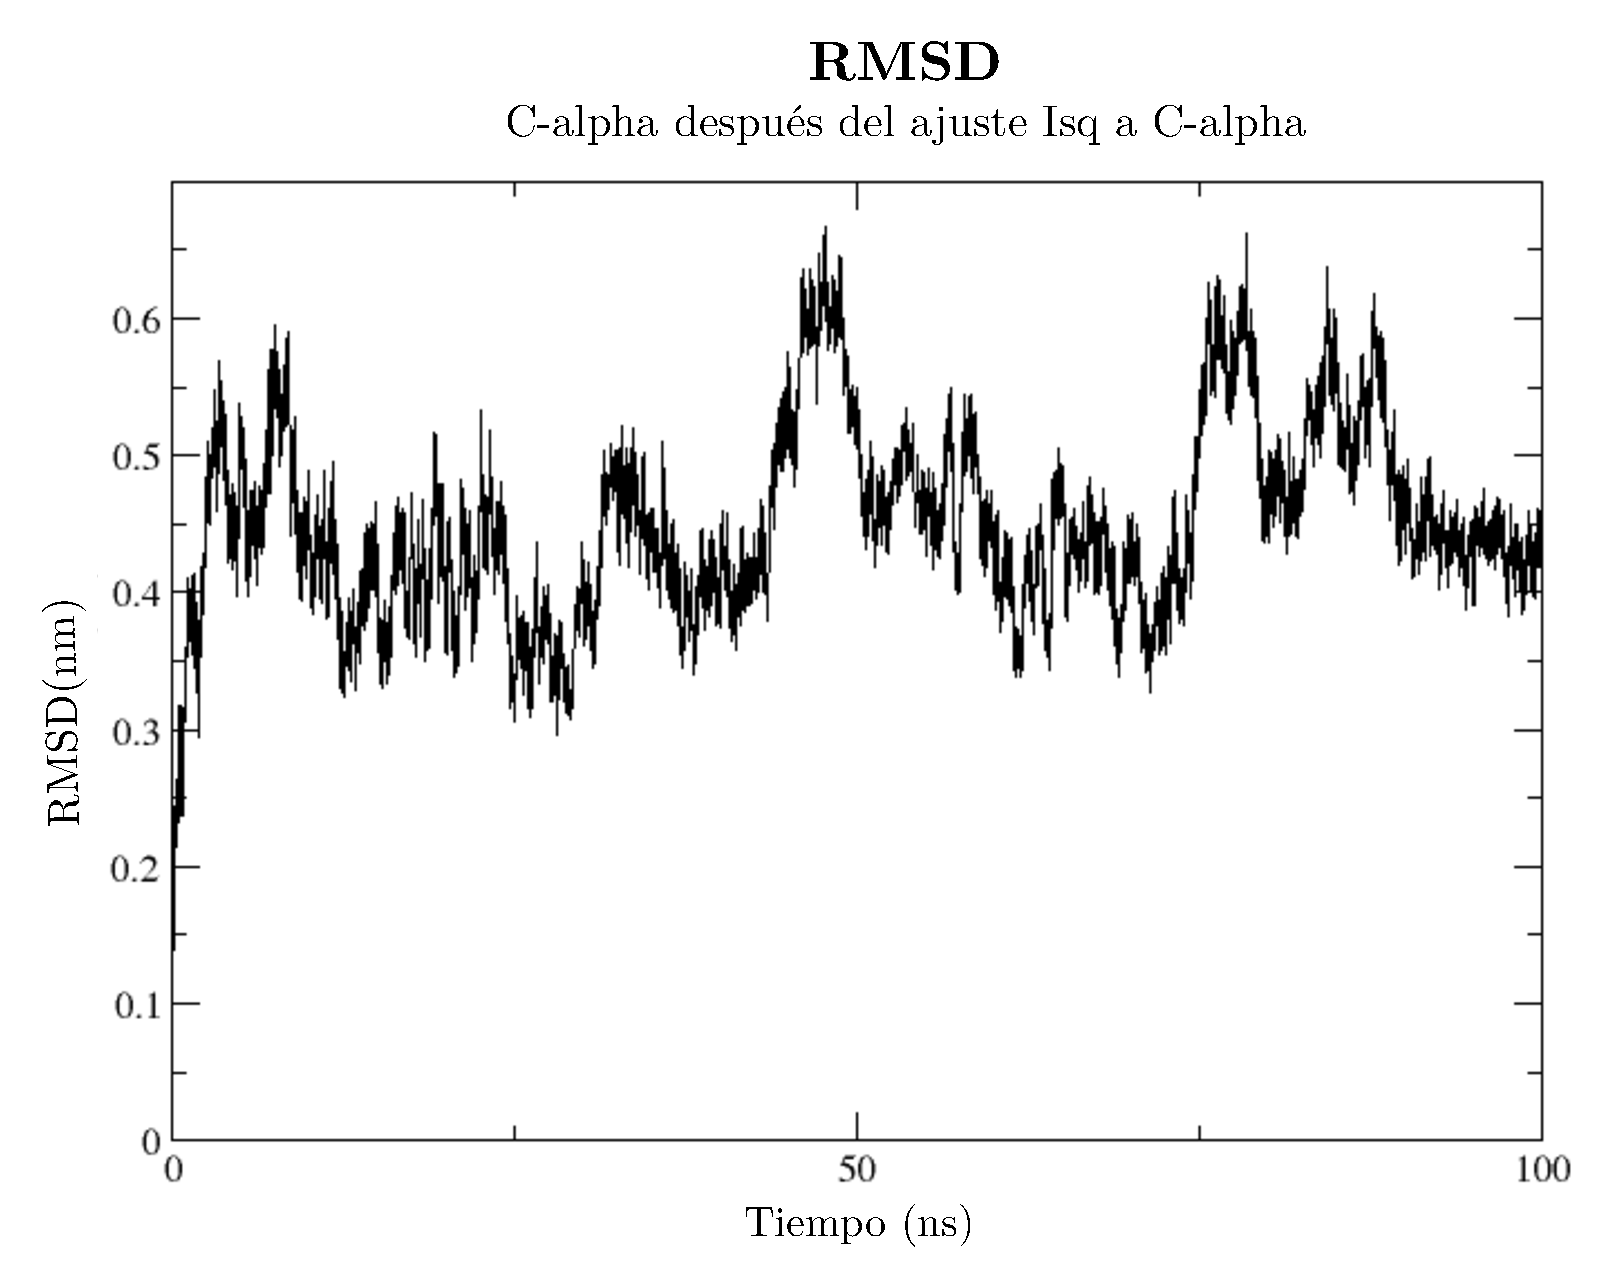
\includegraphics[width=0.82\textwidth]{imagenes/Resu/rmsd-2.pdf}
    \caption{Evolución del RMSD de los átomos C$\alpha$ de la proteína, después del ajuste por mínimos cuadrados a los átomos C$\alpha$ de referencia, durante 100 ns de dinámica molecular.}
    \label{fig:rmsd-2fom}
\end{figure}
        
\begin{figure}[H]
    \centering
    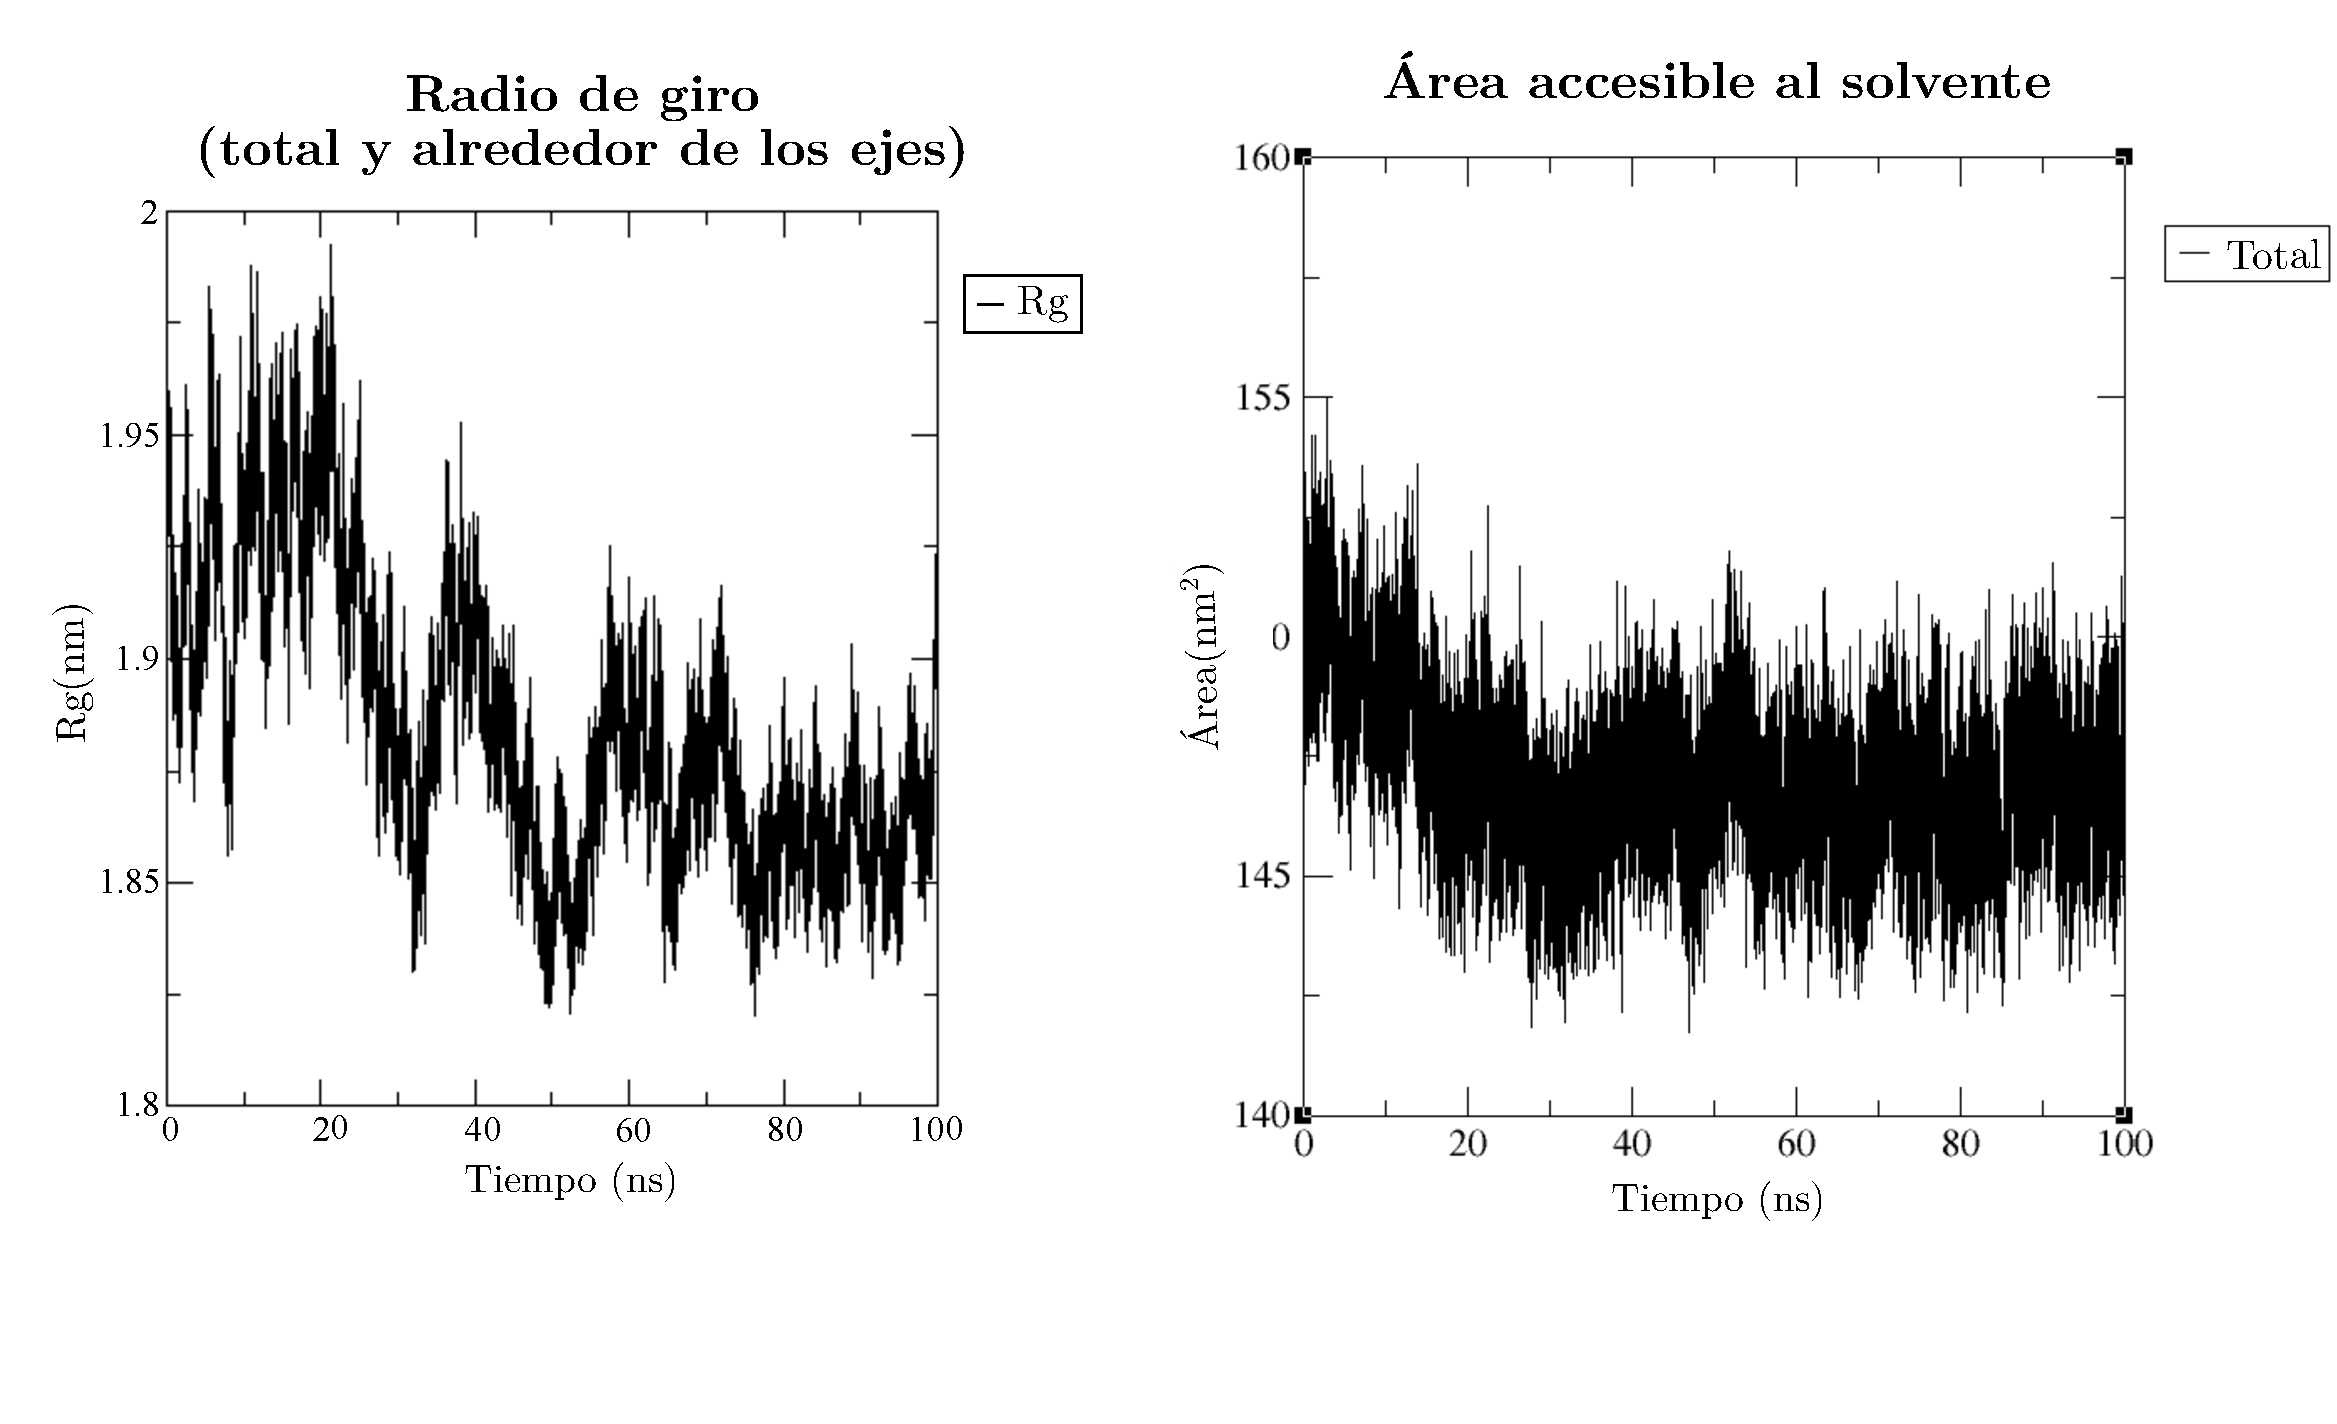
\includegraphics[width=0.95\textwidth]{imagenes/Resu/radio.pdf}
    \caption{Evolución temporal del radio de giro ($R_g$) y del área superficial accesible al solvente ($\text{SASA}$) durante los 100 ns de trayectoria de dinámica molecular.}
    \label{fig:rg-sasa-2fom}
\end{figure} 
      
\begin{figure}[H]
    \centering
    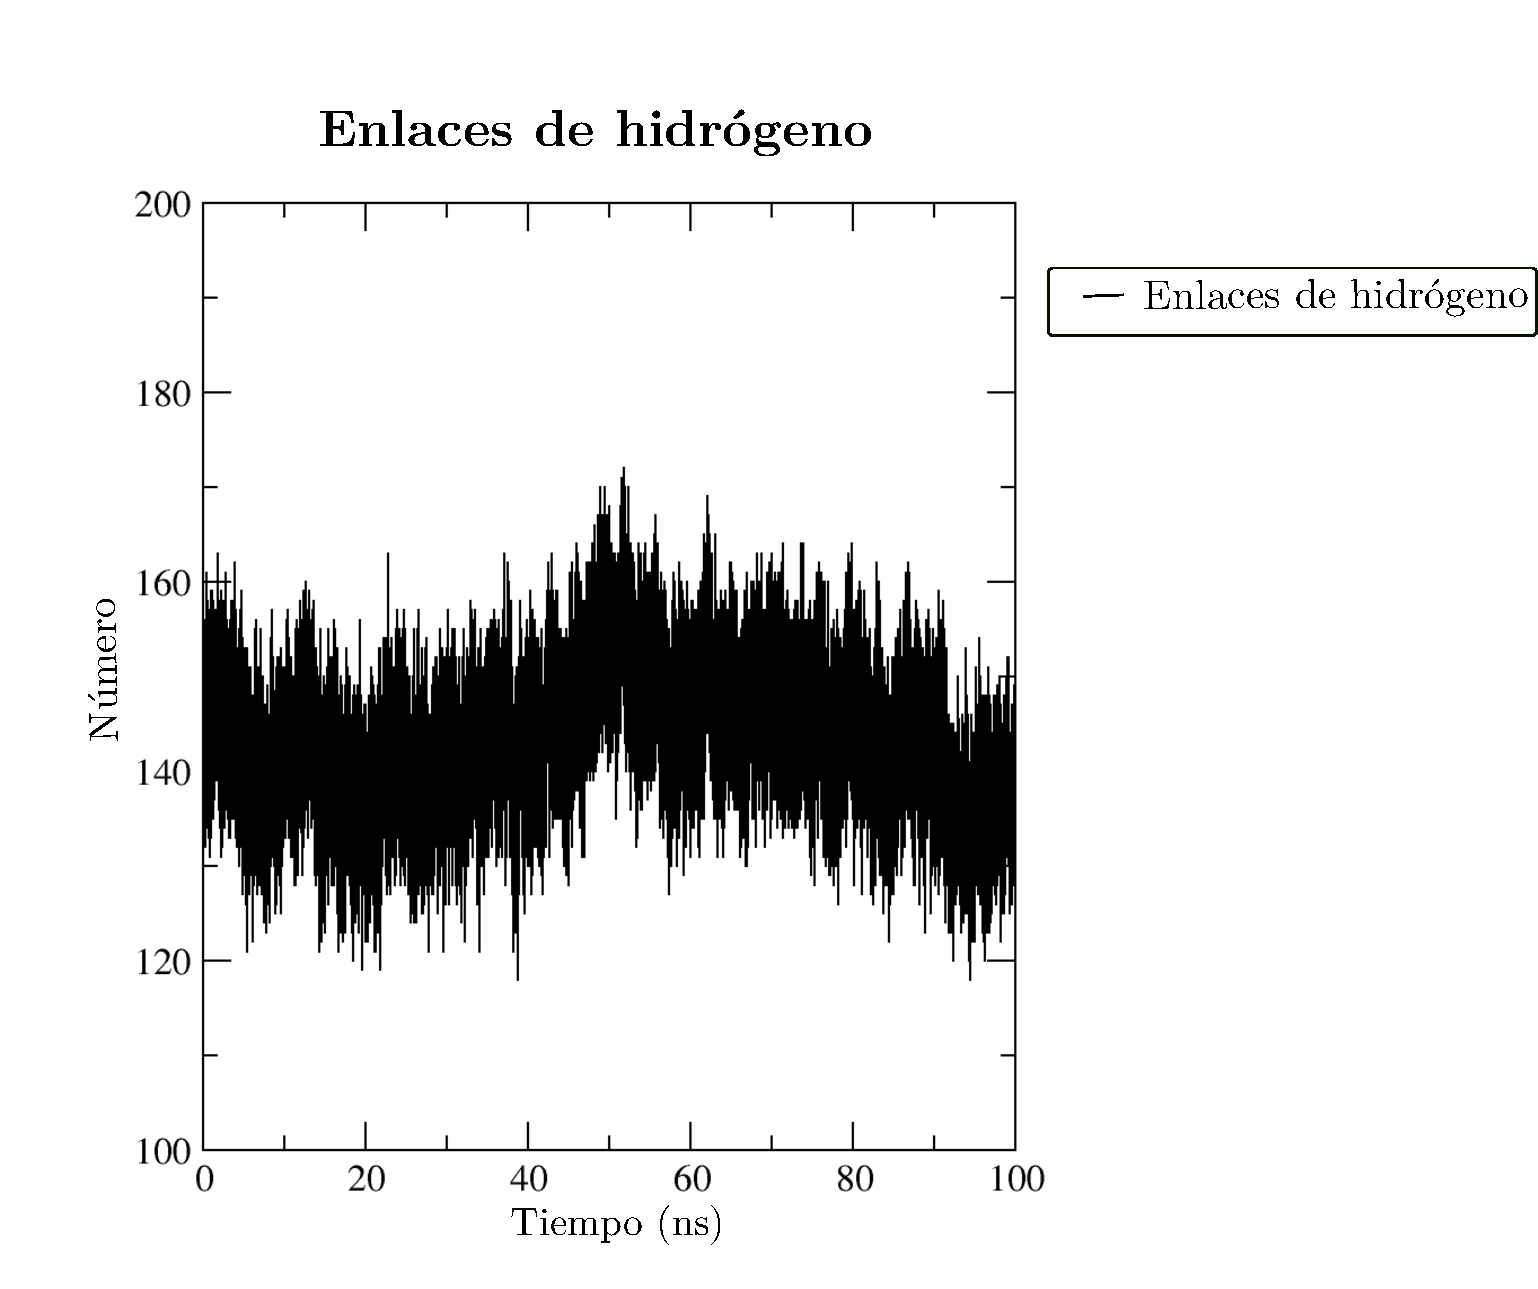
\includegraphics[width=0.70\textwidth]{imagenes/Resu/hidrogeno.pdf}
    \caption{Evolución temporal del número de enlaces de hidrógeno intramoleculares formados en la proteína a lo largo de 100 ns.}
    \label{fig:hbond-2fom}
\end{figure}   

\subsection{Comportamiento de la estabilidad global y movilidad ($\text{RMSD}$)}

Al analizar la evolución de la Desviación Cuadrática Media ($\text{RMSD}$) de los átomos $C\alpha$ (Figura~\ref{fig:rmsd-2fom}), se observa un incremento inicial rápido durante los primeros $5\ \text{ns}$ hasta alcanzar $\sim 0.40\ \text{nm}$, lo cual se atribuye a la acomodación y relajación inicial del sistema en el entorno de solvatación.

Entre los $10$ y $40\ \text{ns}$, la trayectoria exhibe un régimen de equilibrio relativo en torno a $0.40 - 0.45\ \text{nm}$. Sin embargo, entre los $45 - 55\ \text{ns}$ y $75 - 85\ \text{ns}$, se detectan fluctuaciones más marcadas que alcanzan picos de hasta $0.65\ \text{nm}$. Estas variaciones no responden a un proceso de desnaturalización, sino a la notable movilidad intrínseca de la proteína en su estado abierto e inactivo, asociada a los reordenamientos del bucle cofactórico de NS2B y del dominio catalítico. La posterior estabilización del $\text{RMSD}$ en la franja de $0.40 - 0.45\ \text{nm}$ durante los últimos $15\ \text{ns}$ confirma que el sistema convergió hacia una cuenca de energía potencial estable.

\subsection{Proceso de compactación y exposición hidrofóbica ($R_g$ y $\text{SASA}$)}

Los perfiles del Radio de Giro ($R_g$) y del Área Superficial Accesible al Solvente ($\text{SASA}$) (Figura~\ref{fig:rg-sasa-2fom}) respaldan esta interpretación y aportan información sobre el comportamiento macroestructural:

\begin{itemize}
    \item \textbf{Radio de Giro ($R_g$):} A partir del valor inicial de $1.90\ \text{nm}$, se aprecia una expansión transitoria hasta $1.97\ \text{nm}$ en los primeros $15\ \text{ns}$, producto de la apertura de bucles flexibles. No obstante, a partir del nanosegundo $20$ se identifica una tendencia continua hacia la compactación que alcanza un mínimo de $1.82\ \text{nm}$ hacia los $50\ \text{ns}$, para posteriormente mantenerse constante entre $1.84$ y $1.88\ \text{nm}$. Este comportamiento demuestra que la proteína tiende hacia un empaquetamiento más globular con el paso del tiempo.
    
    \item \textbf{Área Accesible al Solvente ($\text{SASA}$):} En concordancia con la contracción del $R_g$, se observa una disminución clara en el $\text{SASA}$ total desde $\sim 155\ \text{nm}^2$ hasta fluctuar en la franja de $145 - 150\ \text{nm}^2$. Esta reducción refleja la ocurrencia de un colapso hidrofóbico interno que minimiza la exposición de los residuos apolares al solvente.
\end{itemize}

\subsection{Dinámica de la red interna de enlaces de hidrógeno}

Al examinar la red de enlaces de hidrógeno intramoleculares (Figura~\ref{fig:hbond-2fom}), se encuentra la explicación molecular a la compactación observada. Se evidencia que la proteasa mantiene de forma constante entre $130$ y $150$ enlaces de hidrógeno internos a lo largo de toda la trayectoria. Destaca un incremento notable en la densidad de estas interacciones entre los $40$ y $60\ \text{ns}$ (con picos de hasta $\sim 165$ contactos), coincidiendo de manera exacta con el mínimo observado en el Radio de Giro ($R_g \approx 1.82\ \text{nm}$).

Este comportamiento demuestra que el fortalecimiento de la red electrostática interna actuó como la fuerza impulsora que consolidó la estructura terciaria frente a la movilidad de los bucles.

En conclusión, la consistencia observada entre la estabilización del $\text{RMSD}$ ($\sim 0.42\ \text{nm}$), la reducción del $R_g$ ($1.85\ \text{nm}$), la disminución del $\text{SASA}$ ($146\ \text{nm}^2$) y la preservación continua de la red de enlaces de hidrógeno intramoleculares permite concluir que la proteasa DENV-2 en conformación abierta e inactiva alcanza una marcada estabilidad estructural bajo las condiciones simuladas.

\begin{figure}[H]
      \centering
      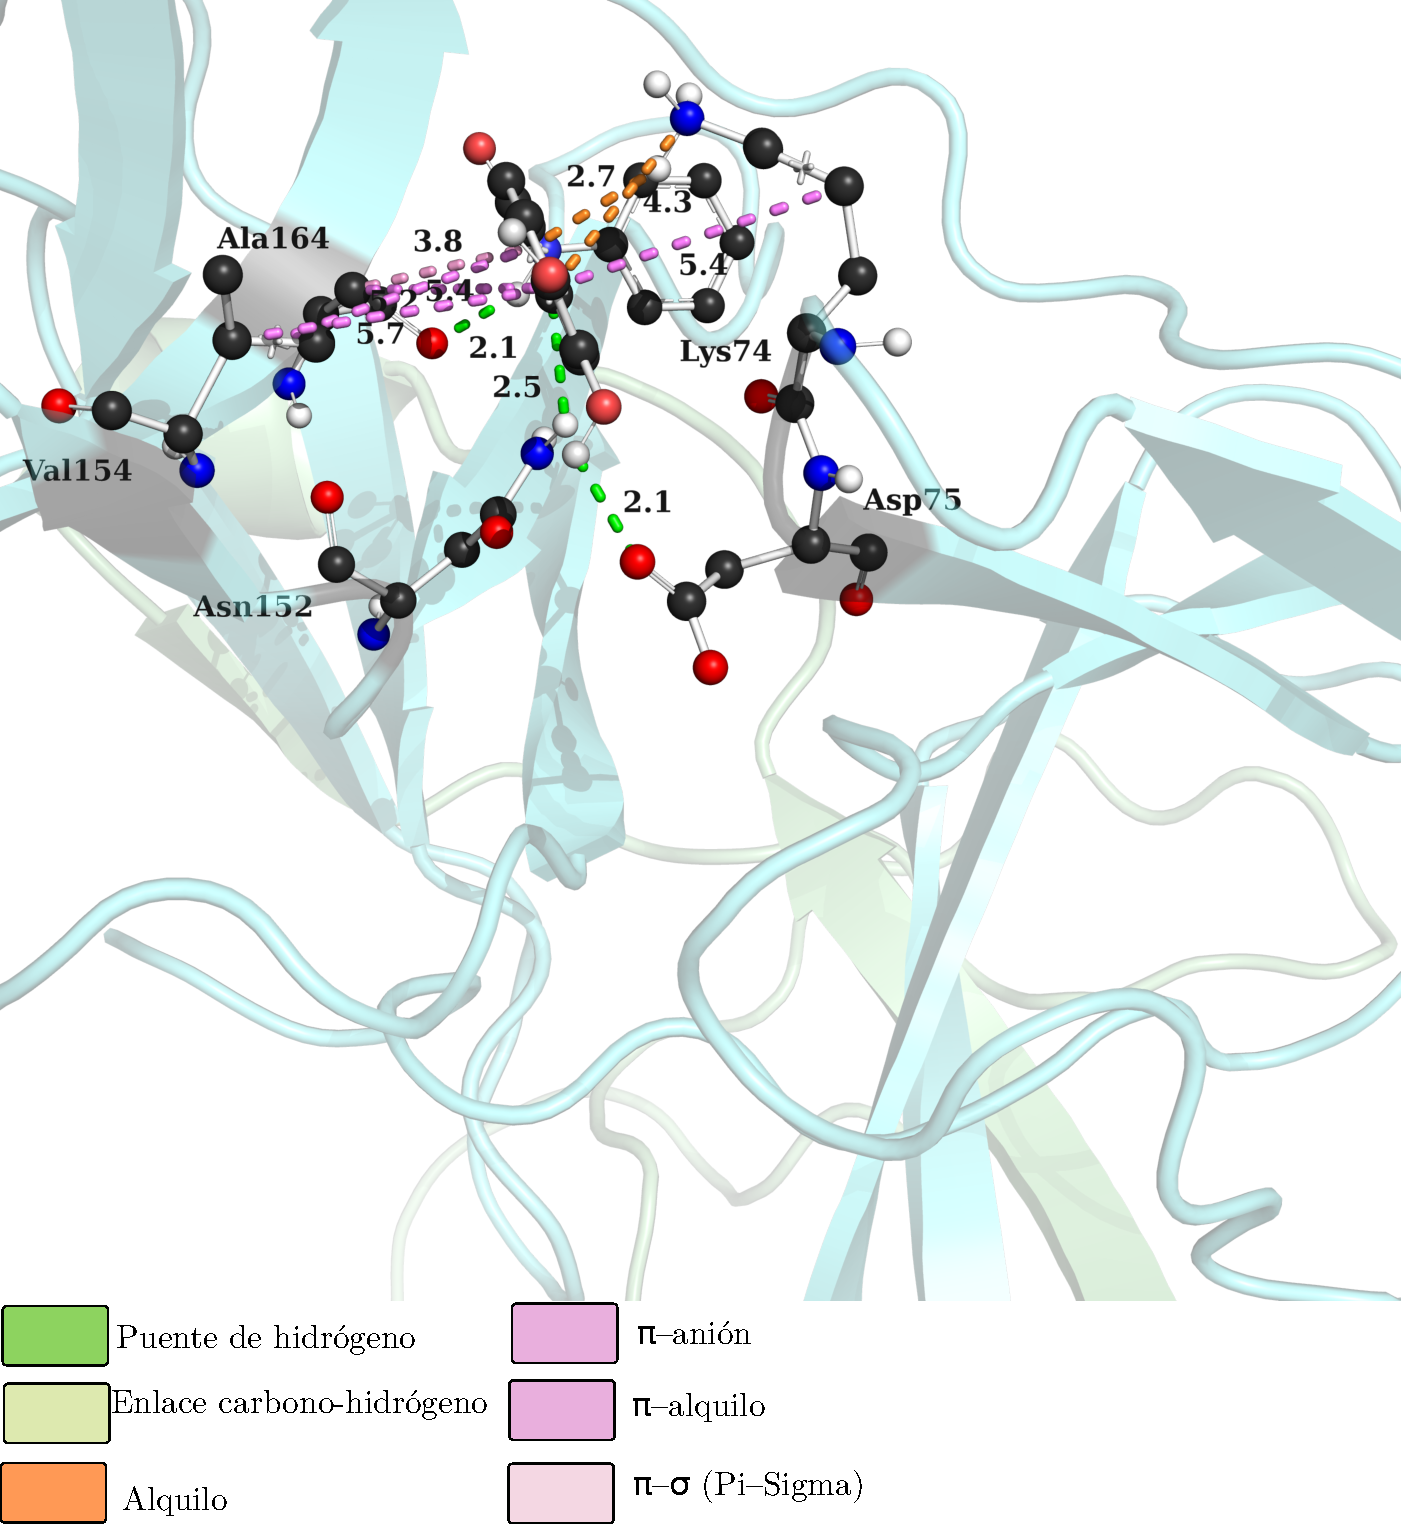
\includegraphics[width=1.0\textwidth]{imagenes/Resu/benza.pdf}
      \caption{Representación 3D del acoplamiento molecular del derivado benzamida en la cavidad alostérica de la proteasa de DENV-2 (Pose 61). Se presentan las distancias de enlace expresadas en ångströms (\AA).}
      \label{fig:mep-gly4}
        \end{figure}

\begin{figure}[H]
      \centering
      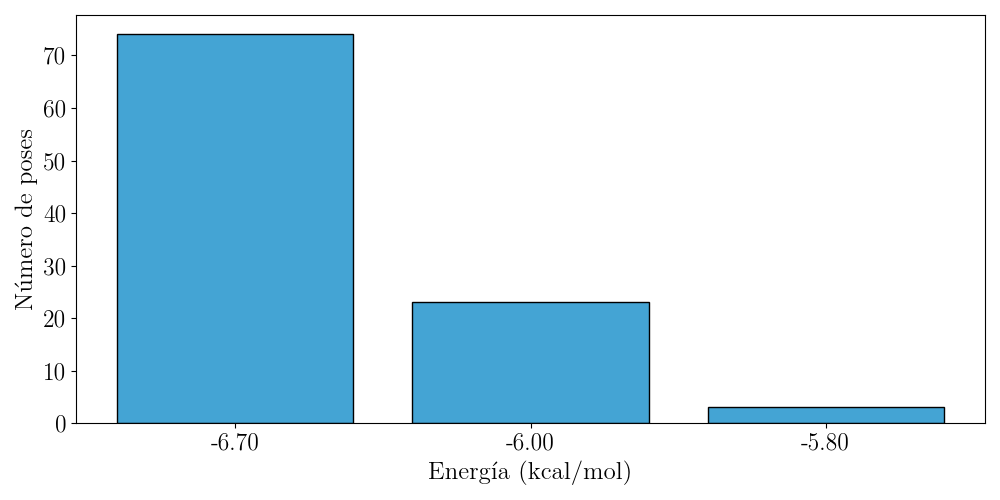
\includegraphics[width=1.0\textwidth]{imagenes/Resu/benza-3.png}
      \caption{M.}
      \label{fig:mep-gly4}
        \end{figure}
        
 \begin{table}[H]
    \centering
    \footnotesize % Tamaño de letra más pequeño para que entre holgadamente
    \setlength{\tabcolsep}{5pt} % Otorga espacio entre columnas para que no se peguen
    \renewcommand{\arraystretch}{1.2}
    \caption{Interacciones no covalentes y distancias de contacto para el acoplamiento del inhibidor alostérico derivado de benzamida en la proteasa de DENV-2 (PDB: 2FOM).}
    \label{tab:interacciones-2fom}
    \begin{tabular}{llcll}
        \toprule
        \multicolumn{1}{c}{\textbf{\shortstack[c]{Tipo de\\interacción}}} & 
        \multicolumn{1}{c}{\textbf{Residuo}} & 
        \multicolumn{1}{c}{\textbf{\shortstack[c]{Distancia\\(\AA)}}} & 
        \multicolumn{1}{c}{\textbf{\shortstack[c]{Motivo\\estructural}}} & 
        \multicolumn{1}{c}{\textbf{\shortstack[c]{Tipo de\\aminoácido}}} \\
        \midrule
        Puente de hidrógeno & Ala164 & 2.07 & Sitio de unión & Apolar / Hidrofóbico \\
                            & Asn152 & 2.52 & Sitio de unión & Polar no cargado \\
                            & Asp75  & 2.12 & Tríada catalítica & Polar, cargado negativo \\
        \midrule
        $\pi$-Catión        & Lys74  & 2.62 & Bolsillo S1 / Sitio activo & Polar, cargado positivo \\
                            & Lys74  & 4.27 & Bolsillo S1 / Sitio activo & Polar, cargado positivo \\
        \midrule
        Interacción hidrofóbica & Val154 & 4.91 & Bolsillo hidrofóbico & Apolar / Hidrofóbico \\
                                & Val154 & 5.16 & Bolsillo hidrofóbico & Apolar / Hidrofóbico \\
                                & Val154 & 5.40 & Bolsillo hidrofóbico & Apolar / Hidrofóbico \\
        \bottomrule
    \end{tabular}
\end{table}
      Se seleccionó la conformación de menor energía ($-6.00 \text{ kcal/mol}$) por presentar el anclaje mediante puente de hidrógeno con el residuo Gly133 del hueco oxianiónico, permitiendo evaluar mediante Dinámica Molecular la estabilidad temporal de esta interacción. 

con un limite de 5.0 y una exaustividad de 80, -6.70 kcal/mol con 74 modelos, otra con -5.80 kcal/mol con 3 modelos y -6.00 kcal/mol con 23 modelos, segun la literatura, estos son los sitios donde se une. 

Como se observa en el perfil energético de la Figura~9.11, el acoplamiento molecular exhibió una marcada convergencia conformacional. La conformación de menor energía libre de unión alcanzó un valor de $-6.70\ \text{kcal/mol}$, concentrando un 74\% del total de las poses generadas. Destacando la estabilidad del complejo ligando-proteína y sugiere que el modo de unión es una pose termodinámicamente favorable en el bolsillo alostérico.
Al contrastar los contactos atómicos obtenidos (Tabla~9.5 y Figura~2D/3D) con los hallazgos reportados en la literatura para inhibidores alostéricos de estructura similar (como el derivado de benzofurano 34e, $\text{IC}_{50} = 0.69\ \mu\text{M}$), se identifican importantes coincidencias estructurales y mecanísticas:

\begin{itemize}
    \item \textbf{Red de Puentes de Hidrógeno y el ``Interruptor Molecular'' (\textbf{Asn152}):} En nuestros resultados, el oxígeno del anillo de benzofurano establece un puente de hidrógeno convencional con la cadena lateral de \textbf{Asn152} a una distancia de $2.52\ \text{\AA}$. Este hallazgo es de vital relevancia, ya que la literatura señala a \textbf{Asn152} como un ``interruptor molecular'' clave responsable de mantener a la enzima en su conformación inactiva. Adicionalmente, el grupo hidroxilo del anillo aromático forma un puente de hidrógeno fuerte de $2.12\ \text{\AA}$ con \textbf{Asp75} (perteneciente a la tríada catalítica), mientras que el grupo N--H de la amida interactúa mediante un enlace de hidrógeno de $2.07\ \text{\AA}$ con el esqueleto de \textbf{Ala164}. Esta red tripartita de puentes de hidrógeno ancla firmemente el ligando al sitio de unión.
    
    \item \textbf{Interacciones Electrostáticas y $\pi$-Catiónicas con \textbf{Lys74}:} La literatura reporta que en derivados como el 34e, la orientación inclinada (\textit{tilted}) del núcleo aromático y el carbonilo amídico permite una interacción crítica con \textbf{Lys74}. En nuestros cálculos de \textit{docking}, se confirmó la participación activa de este residuo mediante dos interacciones de tipo $\pi$-catión con el sistema aromático del compuesto a distancias de $2.62\ \text{\AA}$ y $4.27\ \text{\AA}$. Esta atracción electrostática refuerza la fijación del andamio (\textit{scaffold}) en la entrada del bolsillo S1/alostérico.
    
    \item \textbf{Complementariedad en el Subbolsillo Hidrofóbico:} El análisis de contactos no polares reveló interacciones de tipo $\pi$-sigma y $\pi$-alquil entre el sistema aromático y el residuo \textbf{Val154} ($4.91\ \text{\AA}$, $5.16\ \text{\AA}$ y $5.40\ \text{\AA}$). Aunque los estudios reportados previamente destacan la inserción lipofílica hacia residuos como \textbf{Leu76}, \textbf{Gly148} e \textbf{Ile165}, el contacto hallado con \textbf{Val154} demuestra una acomodación hidrofóbica equivalente que estabiliza el núcleo aromático dentro de la cavidad no polar.
\end{itemize}

Los datos \textit{in silico} obtenidos respaldan el mecanismo de inhibición alostérica no competitiva previamente sustentado por estudios cinéticos ($K_i$) y de mutagénesis dirigida (T122C). Al alojarse en la cavidad posterior cerca del residuo \textbf{Thr122} e interactuar directamente con la tríada catalítica (\textbf{Asp75}) y los residuos de control conformacional (\textbf{Asn152} y \textbf{Lys74}), el ligando bloquea la flexibilidad funcional requerida para el procesamiento del sustrato poliproteico.

En conjunto, la consistencia entre los valores de energía observados, la baja distancia de los puentes de hidrógeno ($\le 2.52\ \text{\AA}$) y la concordancia con los residuos clave descritos en la literatura ratifican la efectividad del \textit{scaffold} evaluado como un candidato promisorio para el desarrollo de fármacos antivirales selectivos contra DENV-2.
 
 \begin{figure}[H]
      \centering
      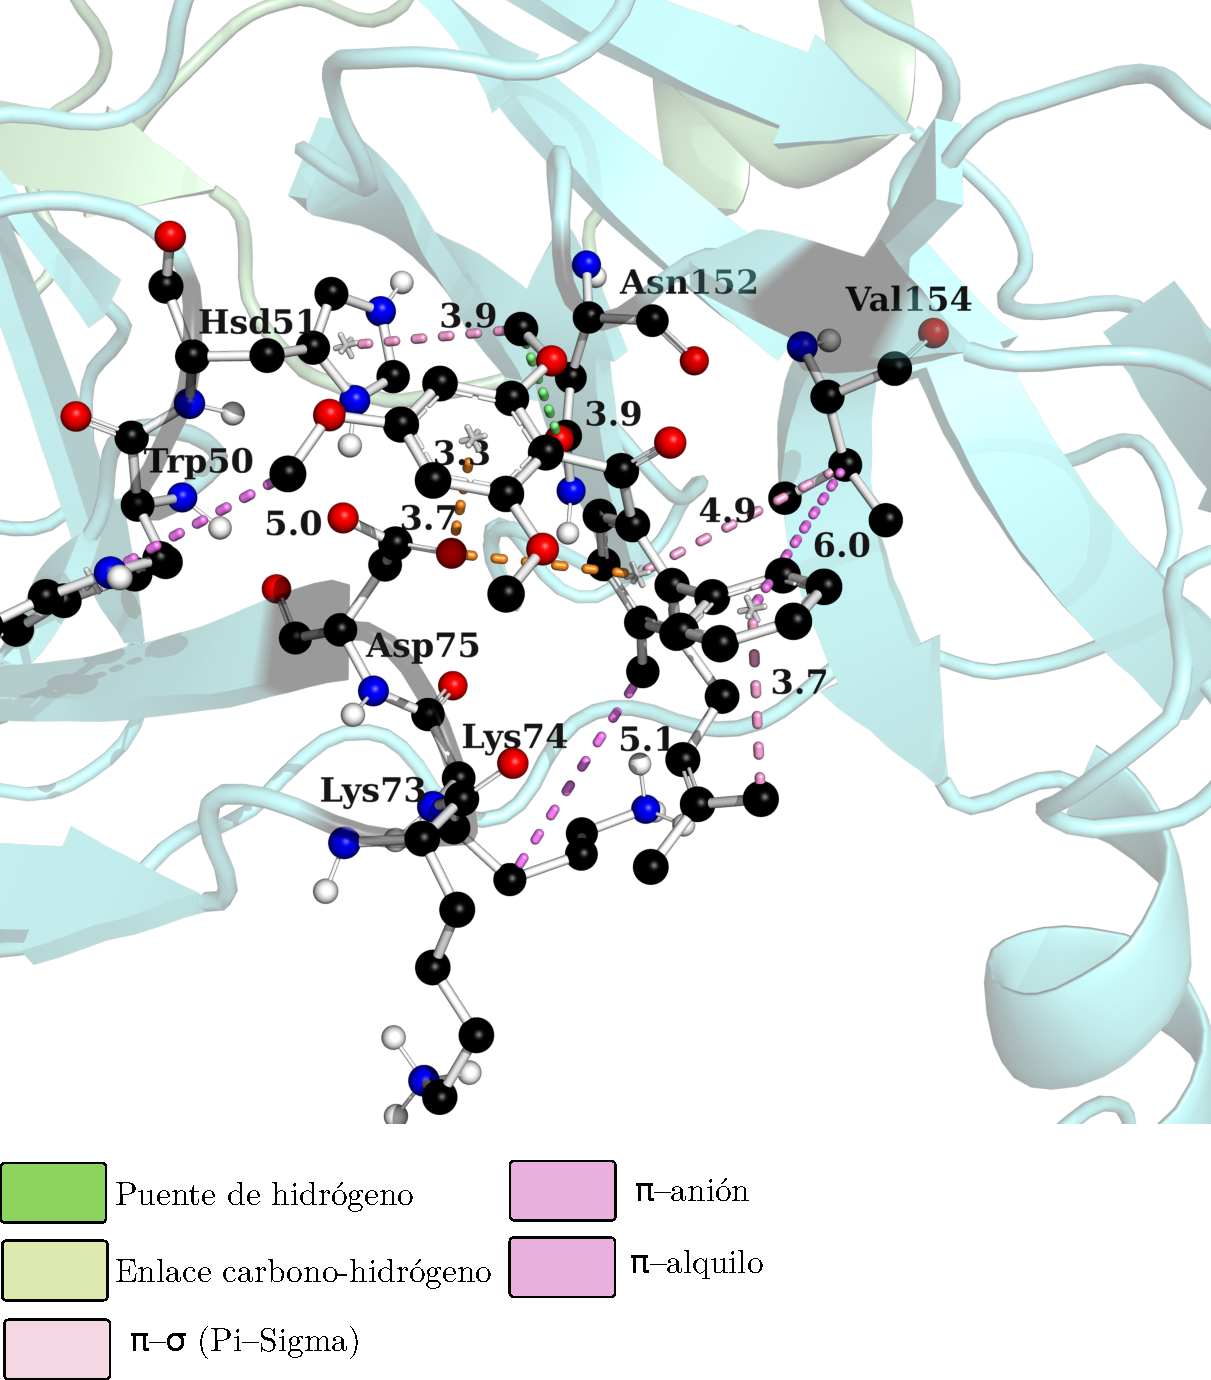
\includegraphics[width=1.0\textwidth]{imagenes/Resu/246.pdf}
      \caption{Representación 3D del acoplamiento molecular del derivado 246D  en la cavidad ortostérica de la proteasa de DENV-2 (Pose 03). Se presentan las distancias de enlace expresadas en ångströms (\AA).}
      \label{fig:mep-gly4}
        \end{figure}
       
\begin{figure}[H]
      \centering
      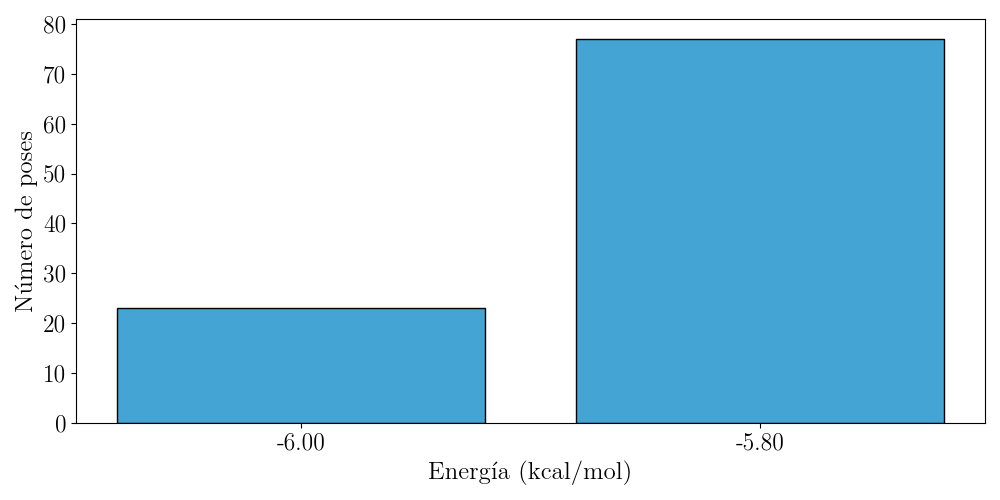
\includegraphics[width=1.0\textwidth]{imagenes/Resu/246-1.png}
      \caption{M.}
      \label{fig:mep-gly4}
        \end{figure}

  \begin{table}[H]
    \centering
    \footnotesize
    \setlength{\tabcolsep}{5pt}
    \renewcommand{\arraystretch}{1.2}
    \caption{Interacciones no covalentes y distancias de contacto para el acoplamiento del inhibidor orto 264 en la proteína de DENV-2 (PDB: 2FOM).}
    \label{tab:interacciones-pose83}
    \begin{tabular}{llcll}
        \toprule
        \multicolumn{1}{c}{\textbf{\shortstack[c]{Tipo de\\interacción}}} & 
        \multicolumn{1}{c}{\textbf{Residuo}} & 
        \multicolumn{1}{c}{\textbf{\shortstack[c]{Distancia\\(\AA)}}} & 
        \multicolumn{1}{c}{\textbf{\shortstack[c]{Motivo\\estructural}}} & 
        \multicolumn{1}{c}{\textbf{\shortstack[c]{Tipo de\\aminoácido}}} \\
        \midrule
        Enlace de H de carbono & Asn152 & 3.76 & Sitio de unión & Polar no cargado \\
        \midrule
        $\pi$-Anión            & Asp75  & 3.28 & Tríada catalítica & Polar, cargado negativo \\
                               & Asp75  & 3.88 & Tríada catalítica & Polar, cargado negativo \\
        \midrule
        $\pi$-Sigma            & Val154 & 3.07 & Bolsillo hidrofóbico & Apolar / Hidrofóbico \\
                               & Hsd51  & 3.85 & Tríada catalítica & Polar, cargado positivo \\
        \midrule
        Interacción hidrofóbica & Trp50  & 4.03 & Bolsillo hidrofóbico & Apolar / Aromático \\
        (Alquil / $\pi$-Alquil) & Lys74  & 4.42 & Bolsillo S1 / Sitio activo & Polar, cargado positivo \\
                               & Val154 & 4.72 & Bolsillo hidrofóbico & Apolar / Hidrofóbico \\
                               & Val154 & 5.32 & Bolsillo hidrofóbico & Apolar / Hidrofóbico \\
        \bottomrule
    \end{tabular}
\end{table}




El análisis del acoplamiento molecular realizado mediante el programa AutoDock Vina (configurado con una exhaustividad de 80) permitió evaluar la afinidad y el modo de unión del ligando en el sitio catalítico del receptor. A partir de una muestra de 100 poses generadas, el perfil energético reveló la presencia de dos conformaciones principales: un primer grupo de 23 poses con una energía libre de unión de $-6.00\ \text{kcal/mol}$ y un segundo conglomerado (\textit{cluster}) predominante correspondiente a 77 poses con una energía de $-5.80\ \text{kcal/mol}$ (Figura~9.1.b).

A pesar de que el primer grupo presentó el valor de energía mínimo absoluto, la selección final del modo de acoplamiento recayó en la \texttt{pose03.pdb} (perteneciente al \textit{cluster} de $-5.80\ \text{kcal/mol}$). Esta decisión se fundamenta en un criterio estadístico y termodinámico: la representación poblacional del 77\% sugiere una mayor probabilidad de ocurrencia del estado conformacional en equilibrio. Además, la diferencia energética de apenas $\Delta E = 0.2\ \text{kcal/mol}$ entre ambos mínimos se encuentra bien dentro del margen del ruido térmico ($k_B T \approx 0.6\ \text{kcal/mol}$ a temperatura ambiente), lo que demuestra que ambas poses son energéticamente equivalentes pero la \texttt{pose03.pdb} es representativa de la microconformación más probable.

La inspección visual y la caracterización de los contactos no covalentes efectuada en PyMOL y Discovery Studio Visualizer (Cuadro~9.5 y Figura~9.1.3) permitieron identificar el patrón de interacciones que estabiliza dicho complejo:

\begin{itemize}
    \item \textbf{Enlaces de Carbono-Hidrógeno y contactos polares:} Se observaron interacciones fuertemente estabilizadoras mediadas por enlaces de carbono-hidrógeno, destacando el papel del residuo polar no cargado \textbf{Asn152}. Este residuo actúa como un ancla clave en la cavidad al interaccionar directamente con los átomos de carbono-hidrógeno del ligando a distancias cortas de contacto.
    \item \textbf{Interacciones electrostáticas y relativas a electrones $\pi$:} Se identificaron interacciones del tipo $\pi$-anión y $\pi$-sigma con los residuos de la tríada catalítica y del contorno del sitio activo (\textbf{His51}, \textbf{Asp75} y \textbf{Lys74}), así como contactos hidrofóbicos ($\pi$-alquilo / alquilo) con residuos como \textbf{Val154} y \textbf{Trp50}.
\end{itemize}

Al contrastar nuestros resultados con el estudio de referencia reportado por literatura para el inhibidor sintético 246DA ($K_i = 19.84\ \mu\text{M}$) acoplado en la proteasa NS2B/NS3 del serotipo 2 del virus del dengue (PDB ID: \textbf{2FOM}, resolución de $1.5\ \text{\AA}$), se observa una coincidencia estructural y funcional sobresaliente. En la literatura se reporta que la potencia del compuesto 246DA radica en su capacidad para interaccionar mediante puentes de hidrógeno directos con la tríada catalítica (\textbf{His51}, \textbf{Asp75} y \textbf{Ser135}), a la vez que ocupa el bolsillo hidrofóbico coordinándose con residuos como \textbf{Leu76}, \textbf{Trp83}, \textbf{Ile165} e \textbf{Ile166}. 

Nuestras observaciones reafirman que la \texttt{pose03.pdb} adopta una orientación tridimensional coherente con dicho modelo bioactivo. Aunque nuestro acoplamiento con AutoDock Vina prioriza las fuerzas de Van der Waals, electrostáticas y enlaces C--H con residuos como \textbf{Asn152}, \textbf{His51} y \textbf{Asp75}, la conservación del anclaje en los residuos de la tríada catalítica confirma la validez biológica del acoplamiento. Esto sugiere que el complejo obtenido reproduce los requerimientos farmacofóricos necesarios para la inhibición competitiva de la proteasa viral DEN2.
    
\begin{figure}[H]
      \centering
      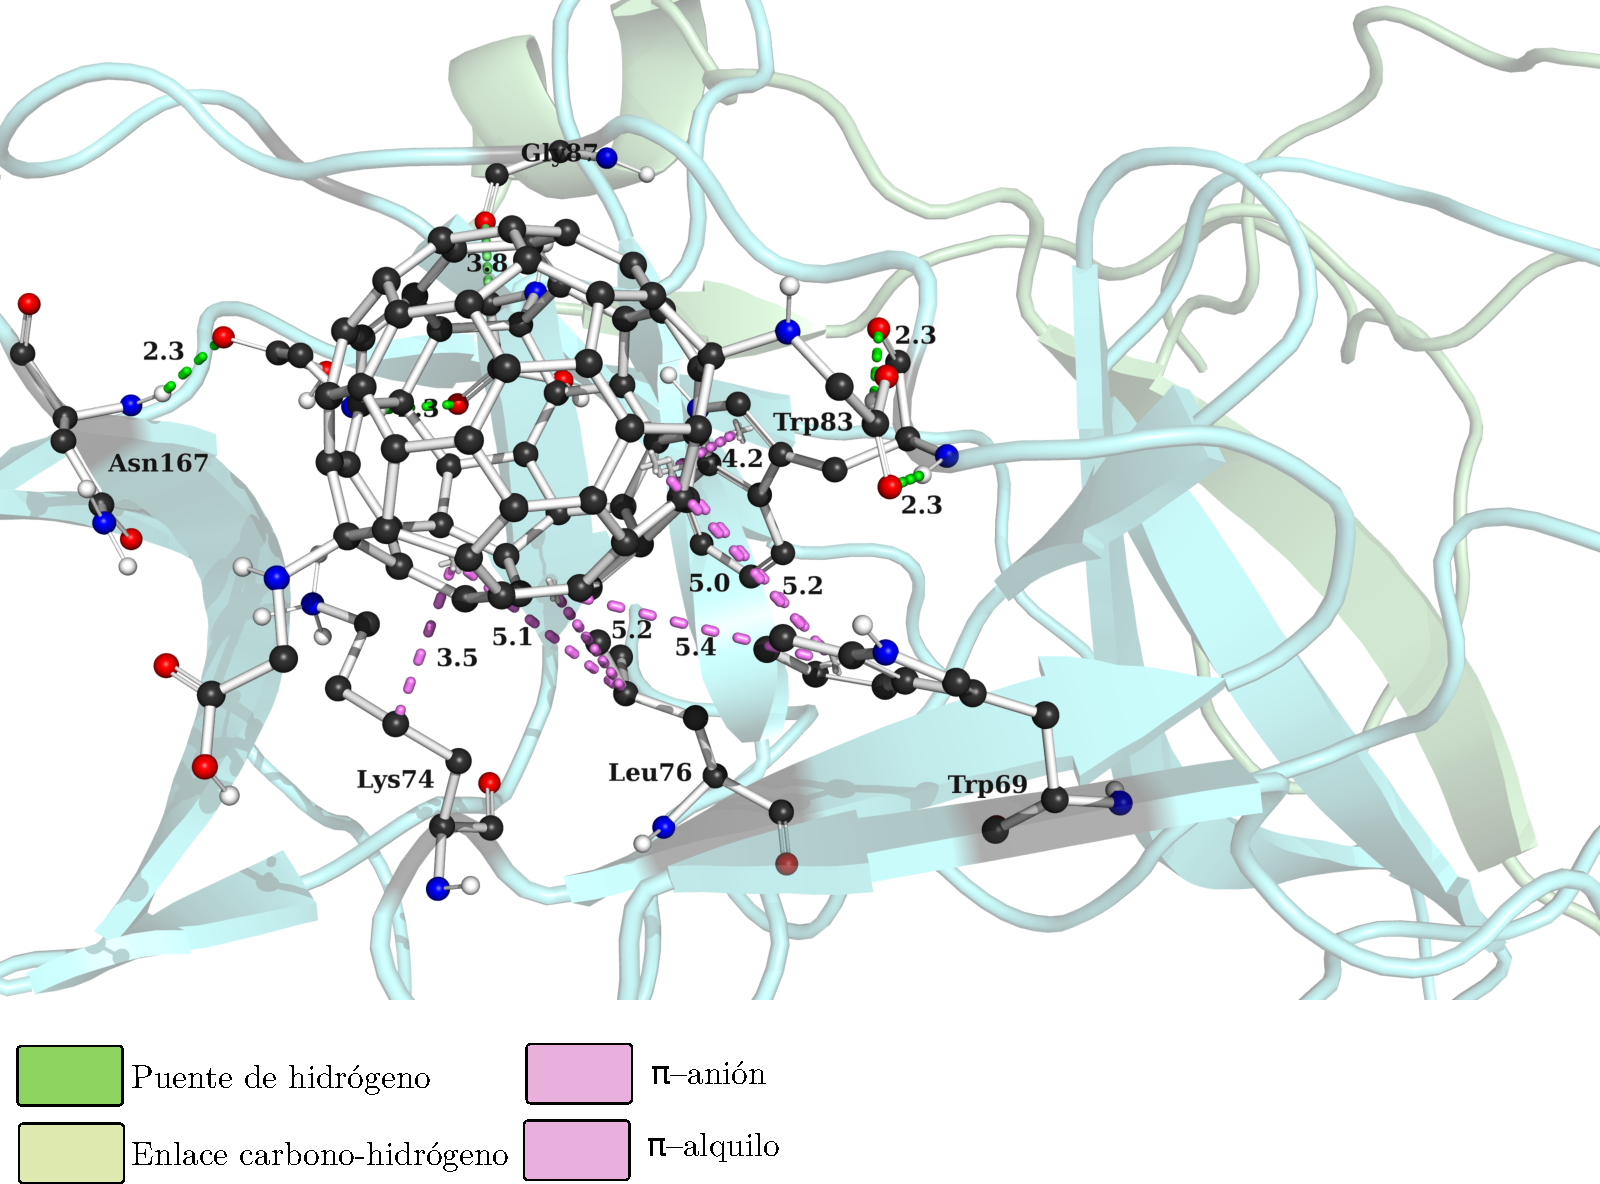
\includegraphics[width=1.0\textwidth]{imagenes/Resu/ciego.pdf}
      \caption{M.}
      \label{fig:mep-gly4}
        \end{figure}
        
\begin{figure}[H]
      \centering
      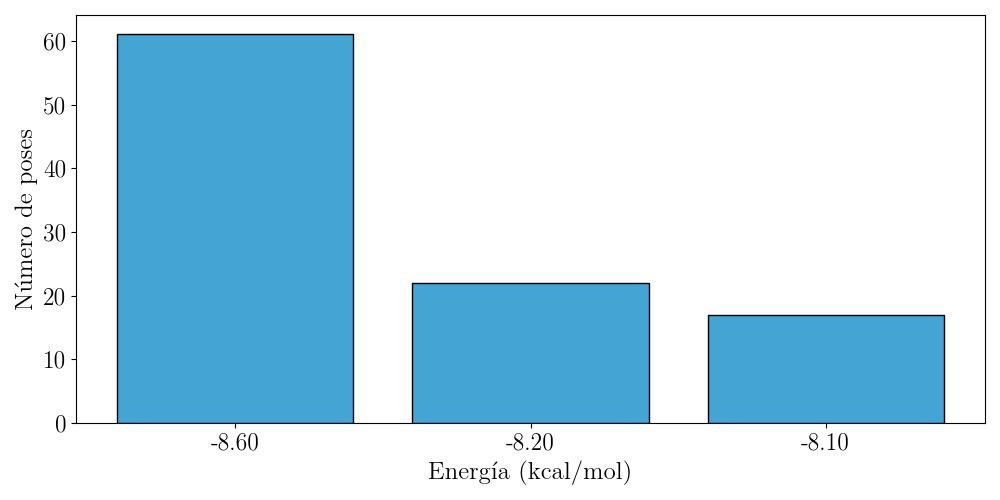
\includegraphics[width=1.0\textwidth]{imagenes/Resu/ciego.png}
      \caption{M.}
      \label{fig:mep-gly4}
        \end{figure}
        
   \begin{table}[H]
    \centering
    \footnotesize
    \setlength{\tabcolsep}{5pt}
    \renewcommand{\arraystretch}{1.2}
    \caption{Interacciones no covalentes y distancias de contacto para el acoplamiento ciego del derivado de fullereno C\textsubscript{60}(Gly)\textsubscript{4} en la proteasa de DENV-2 (PDB: 2FOM, Pose 72).}
    \label{tab:interacciones-pose72}
    \begin{tabular}{llcll}
        \toprule
        \multicolumn{1}{c}{\textbf{\shortstack[c]{Tipo de\\interacción}}} & 
        \multicolumn{1}{c}{\textbf{Residuo}} & 
        \multicolumn{1}{c}{\textbf{\shortstack[c]{Distancia\\(\AA)}}} & 
        \multicolumn{1}{c}{\textbf{\shortstack[c]{Motivo\\estructural}}} & 
        \multicolumn{1}{c}{\textbf{\shortstack[c]{Tipo de\\aminoácido}}} \\
        \midrule
        Puente de hidrógeno & Lys74  & 2.92 & Bolsillo S1 / Sitio activo & Polar, cargado positivo \\
        \midrule
        Enlace de H de carbono & Asp174 & 3.26 & Sitio de unión & Polar, cargado negativo \\
                            & Asn167 & 3.40 & Sitio de unión & Polar no cargado \\
                            & Gly48 & 3.78 & Sitio de unión & Apolar / Neutro \\
        \midrule
        Interacción hidrofóbica & Trp83  & 5.24 & Bolsillo hidrofóbico & Apolar / Aromático \\
        ($\pi$-Alquil) & & & & \\
        \bottomrule
    \end{tabular}
\end{table}
     El análisis del acoplamiento ciego (\textit{blind docking}) realizado mediante el programa AutoDock Vina permitió evaluar la capacidad de interacción, la afinidad termodinámica y el modo de unión del derivado de fulereno tetra-aducto de glicina (C\textsubscript{60}(Gly)\textsubscript{4}) sobre la estructura tridimensional de la proteasa NS2B/NS3 del serotipo 2 del virus del dengue (PDB ID: \textbf{2FOM}). A partir de un muestreo de 100 poses generadas, el perfil energético reveló una distribución conformacional dividida en tres conglomerados (\textit{clusters}) principales: un primer grupo mayoritario de 61 poses con una energía libre de unión ($\Delta G$) de $-8.60\ \text{kcal/mol}$, seguido de un segundo grupo de 22 poses con $-8.20\ \text{kcal/mol}$ y un tercer grupo de 17 poses con $-8.10\ \text{kcal/mol}$ (Figura~9.16).

La selección del modo de acoplamiento óptimo recayó en la \texttt{pose72.pdb}, perteneciente al \textit{cluster} con el mínimo energético absoluto de $-8.60\ \text{kcal/mol}$. A diferencia de sistemas donde el mínimo energético y la densidad conformacional divergen, en este caso coinciden ambos criterios: la amplia representación poblacional (61\%) demuestra que esta conformación no solo es la más estable termodinómicamente, sino también  en equilibrio más probable durante el proceso de reconocimiento molecular. Asimismo, el valor atrayente de $-8.60\ \text{kcal/mol}$ refleja una afinidad sustancialmente elevada, favorecida por la naturaleza anfífilica del aducto, el cual combina el núcleo hidrofóbico del fulereno $C_{60}$ con las cadenas polares de glicina.

La caracterización detallada de los contactos no covalentes efectuada mediante PyMOL y Discovery Studio Visualizer (Tabla~9.7 e Ilustración visual) permitió dilucidar el patrón de interacciones responsables de la estabilización del complejo nanoestructura-proteína:

\begin{itemize}
    \item \textbf{Puentes de hidrógeno convencionales:} Se identificó un puente de hidrógeno fuerte entre el grupo carboxilo/amino de las cadenas de glicina del ligando y el residuo \textbf{Lys74} a una distancia de $2.92\ \text{\AA}$. Este contacto en el subsitio S1 / entorno del sitio activo actúa como un ancla electrostática y polar determinante para la orientación del aducto.
    \item \textbf{Enlaces de hidrógeno no convencionales (C--H):} Se detectaron interacciones estabilizadoras débiles tipo $\text{C--H}\cdots\text{O/N}$ con los residuos \textbf{Asp174} ($3.26\ \text{\AA}$), \textbf{Asn167} ($3.40\ \text{\AA}$) y \textbf{Gly48} ($3.78\ \text{\AA}$), las cuales contribuyen a fijar los sustituyentes de glicina a lo largo del contorno de la cavidad de unión.
    \item \textbf{Interacciones hidrofóbicas ($\pi$-Alquil):} El núcleo aromático de la esfera de fulereno establece contactos lipofílicos de tipo $\pi$-alquilo con el residuo aromático \textbf{Trp83} a una distancia de $5.24\ \text{\AA}$, acomodándose adecuadamente dentro del bolsillo hidrofóbico de la proteasa.
\end{itemize}

Al contrastar estos resultados con la literatura reportada para aductos de fulereno-glicina (C\textsubscript{60}(Gly)), se constata una consistencia notable con las propiedades fisicoquímicas y de unión a proteínas descritas experimentalmente. En estudios previos se ha demostrado mediante calorimetría de titulación isotérmica (ITC) que los aductos de C\textsubscript{60}(Gly) presentan una elevada constante de asociación con proteínas séricas humanas ($K_b = 1.3 \times 10^6\ \text{M}^{-1}$), impulsada principalmente por fuerzas hidrofóbicas y solvatación favorable, sin generar efectos citotóxicos ni genotóxicos significativos. De manera análoga, nuestros resultados \textit{in silico} confirman que el C\textsubscript{60}(Gly)\textsubscript{4} posee la versatilidad estructural para insertarse en la cavidad catalítica de la proteasa DEN2 (PDB ID: \textbf{2FOM}), acoplándose simultáneamente al subsitio S1 (\textbf{Lys74}) y al bolsillo hidrofóbico (\textbf{Trp83}).

En conjunto, la conservación de estos anclajes clave y la alta afinidad calculada sugerirían que la \texttt{pose72.pdb} logra ocluir estéricamente el sitio activo de la proteasa NS2B/NS3, validando la hipótesis de que el derivado C\textsubscript{60}(Gly)\textsubscript{4} se comporta como un potencial inhibidor competitivo o nano-plataforma bioactiva contra el virus del dengue serotipo 2.
        
\begin{figure}[H]
      \centering
      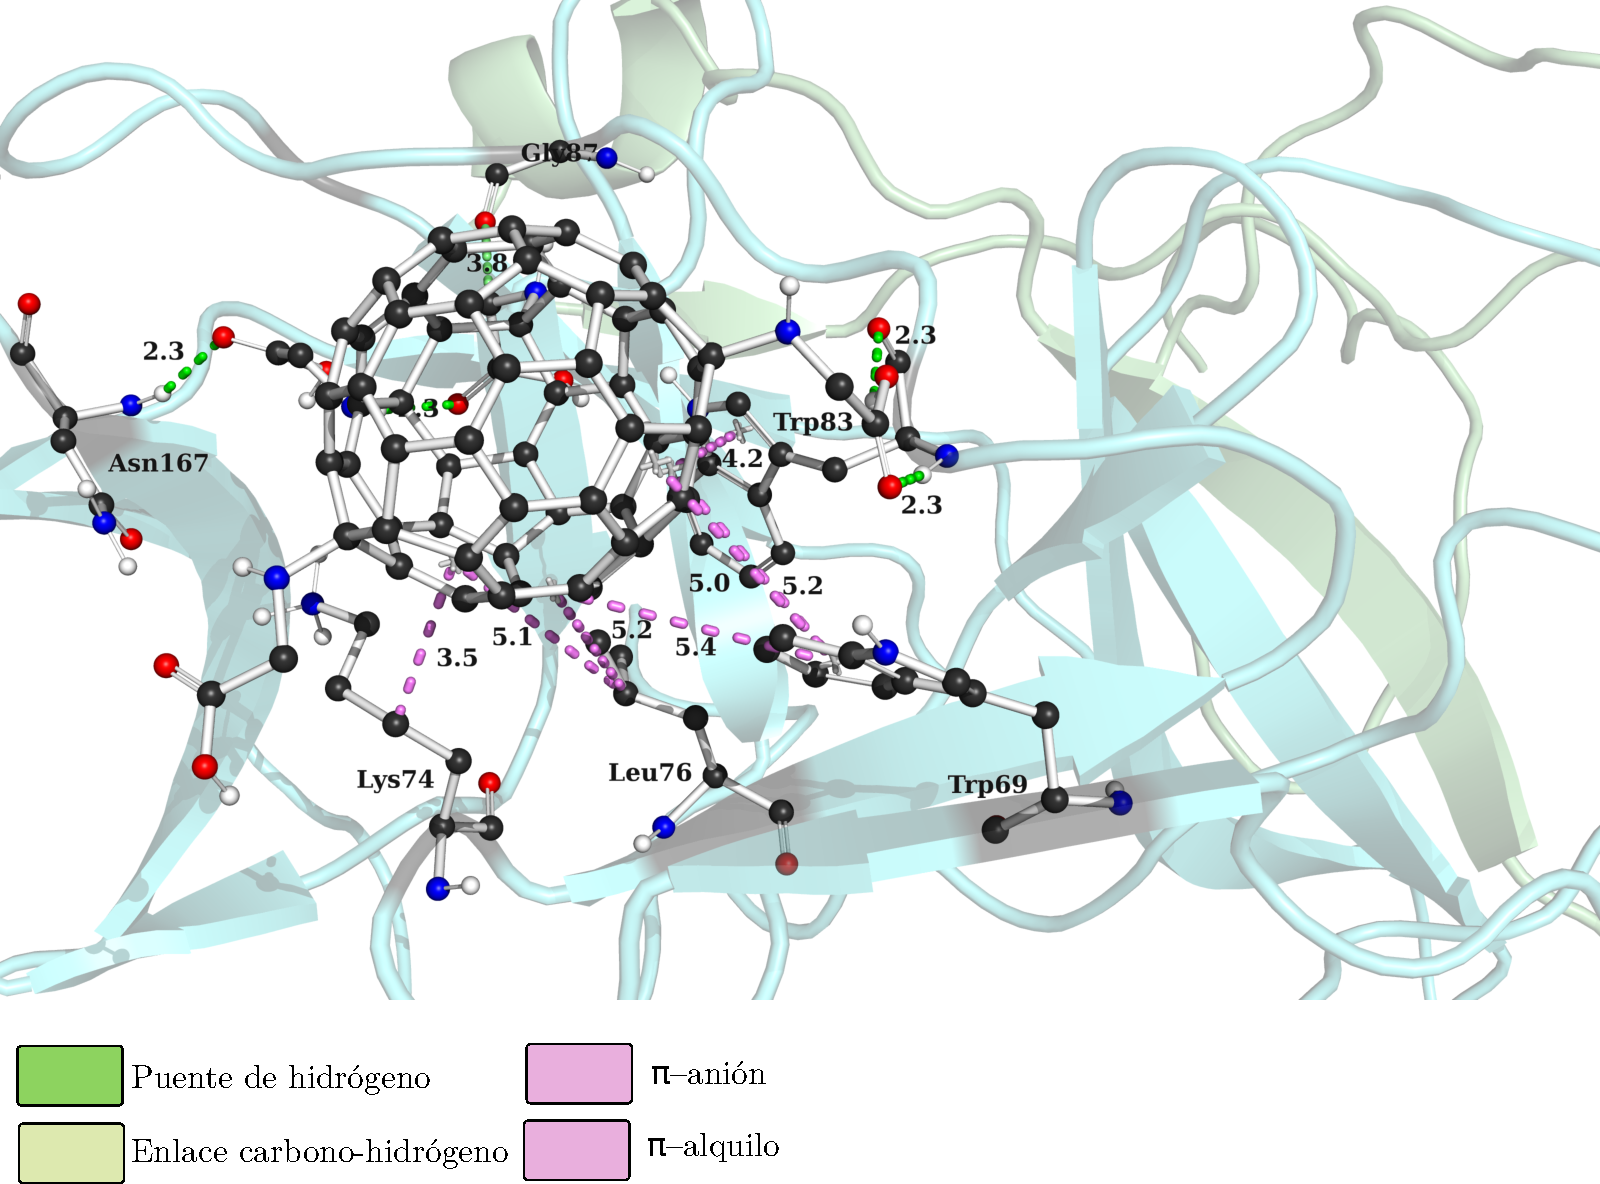
\includegraphics[width=1.0\textwidth]{imagenes/Resu/repor-c60.pdf}
      \caption{M.}
      \label{fig:mep-gly4}
        \end{figure}

\begin{figure}[H]
      \centering
      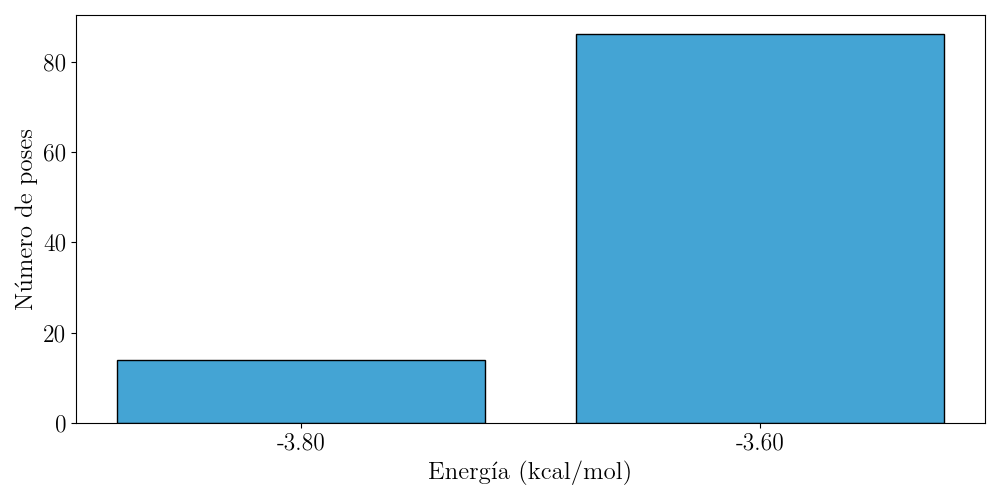
\includegraphics[width=1.0\textwidth]{imagenes/Resu/alo-resu-c60.png}
      \caption{M.}
      \label{fig:mep-gly4}
        \end{figure}
        
 \begin{table}[H]
    \centering
    \footnotesize
    \setlength{\tabcolsep}{5pt}
    \renewcommand{\arraystretch}{1.2}
    \caption{Interacciones no covalentes y distancias de contacto para el acoplamiento del derivado de fullereno C\textsubscript{60}(Gly)\textsubscript{4} en la proteasa de DENV-2 (PDB: 2FOM, Pose 61).}
    \label{tab:interacciones-pose61}
    \begin{tabular}{llcll}
        \toprule
        \multicolumn{1}{c}{\textbf{\shortstack[c]{Tipo de\\interacción}}} & 
        \multicolumn{1}{c}{\textbf{Residuo}} & 
        \multicolumn{1}{c}{\textbf{\shortstack[c]{Distancia\\(\AA)}}} & 
        \multicolumn{1}{c}{\textbf{\shortstack[c]{Motivo\\estructural}}} & 
        \multicolumn{1}{c}{\textbf{\shortstack[c]{Tipo de\\aminoácido}}} \\
        \midrule
        Puente de hidrógeno & Asn167 & 2.34 & Sitio de unión & Polar no cargado \\
                            & Trp83  & 2.32 & Bolsillo hidrofóbico & Apolar / Aromático \\
        \midrule
        Enlace de H de carbono & Gly87  & 3.67 & Sitio de unión & Apolar / Neutro \\
        \midrule
        Interacción hidrofóbica & Leu76  & 4.78 & Bolsillo hidrofóbico & Apolar / Hidrofóbico \\
        (Alquil / $\pi$-Alquil) & Trp69  & 5.22 & Bolsillo hidrofóbico & Apolar / Aromático \\
                                & Lys74  & 6.12 & Bolsillo S1 / Sitio activo & Polar, cargado positivo \\
        \bottomrule
    \end{tabular}
\end{table}       
\subsection{Evaluación del Acoplamiento Alostérico del Derivado $C_{60}(\text{Gly})_4$}

El análisis del acoplamiento molecular dirigido hacia el bolsillo alostérico de la proteasa NS2B/NS3 de DENV-2 (PDB ID: \textbf{2FOM}) se llevó a cabo bajo los mismos parámetros de exhaustividad (80) para evaluar la capacidad del aducto C\textsubscript{60}(Gly)\textsubscript{4} de actuar como un inhibidor alostérico en el sitio reportado para moléculas pequeñas como las benzamidas. A partir del muestreo de 100 poses generadas, el perfil energético (Figura~9.18) mostró una distribución conformacional altamente homogénea pero con valores de afinidad moderados: un grupo de 14 poses con una energía libre de unión de $-3.80\ \text{kcal/mol}$ y un conglomerado predominantemente mayoritario correspondiente a 86 poses con una energía de $-3.60\ \text{kcal/mol}$.

La selección de la modo de acoplamiento recayó en la \texttt{pose61.pdb}, perteneciente al grupo de mínima energía de $-3.80\ \text{kcal/mol}$. La diferencia energética entre ambos mínimos ($\Delta\Delta G = 0.20\ \text{kcal/mol}$) se encuentra holgadamente contenida dentro del margen del ruido térmico ($k_B T \approx 0.60\ \text{kcal/mol}$ a temperatura ambiente), lo que demuestra que ambas poblaciones representan microconformaciones equivalentes en rápido equilibrio termodinámico a lo largo de la entrada de la cavidad alostérica.

La caracterización visual y atómica de las interacciones no covalentes (Tabla~9.8 e Ilustración de contactos) permitió identificar el patrón de estabilización de la \texttt{pose61.pdb}:

\begin{itemize}
    \item \textbf{Puentes de hidrógeno convencionales:} Se observaron dos puentes de hidrógeno fuertes mediados por los sustituyentes de glicina del aducto con la cadena lateral de \textbf{Asn167} ($2.34\ \text{\AA}$, polar no cargado) y con el residuo aromático \textbf{Trp83} ($2.32\ \text{\AA}$), fijando las cadenas polares externas en el contorno del sitio alostérico.
    \item \textbf{Enlaces de hidrógeno de carbono (C--H):} Se identificó un contacto débil tipo $\text{C--H}\cdots\text{O/N}$ entre el esqueleto del ligando y el residuo \textbf{Gly87} a una distancia de $3.67\ \text{\AA}$.
    \item \textbf{Interacciones hidrofóbicas (Alquil / $\pi$-Alquil):} La esfera carbonosa del fulereno interacciona mediante contactos lipofílicos con los residuos \textbf{Leu76} ($4.78\ \text{\AA}$) y \textbf{Trp69} ($5.22\ \text{\AA}$) en el subbolsillo hidrofóbico, además de mantener un contacto de tipo alquilo/electrostático extendido con \textbf{Lys74} ($6.12\ \text{\AA}$).
\end{itemize}

\subsection{Análisis Comparativo entre el Derivado de Fulereno y el Inhibidor Alostérico de Referencia (Benzamida/Benzofurano)}


\begin{figure}[H]
      \centering
      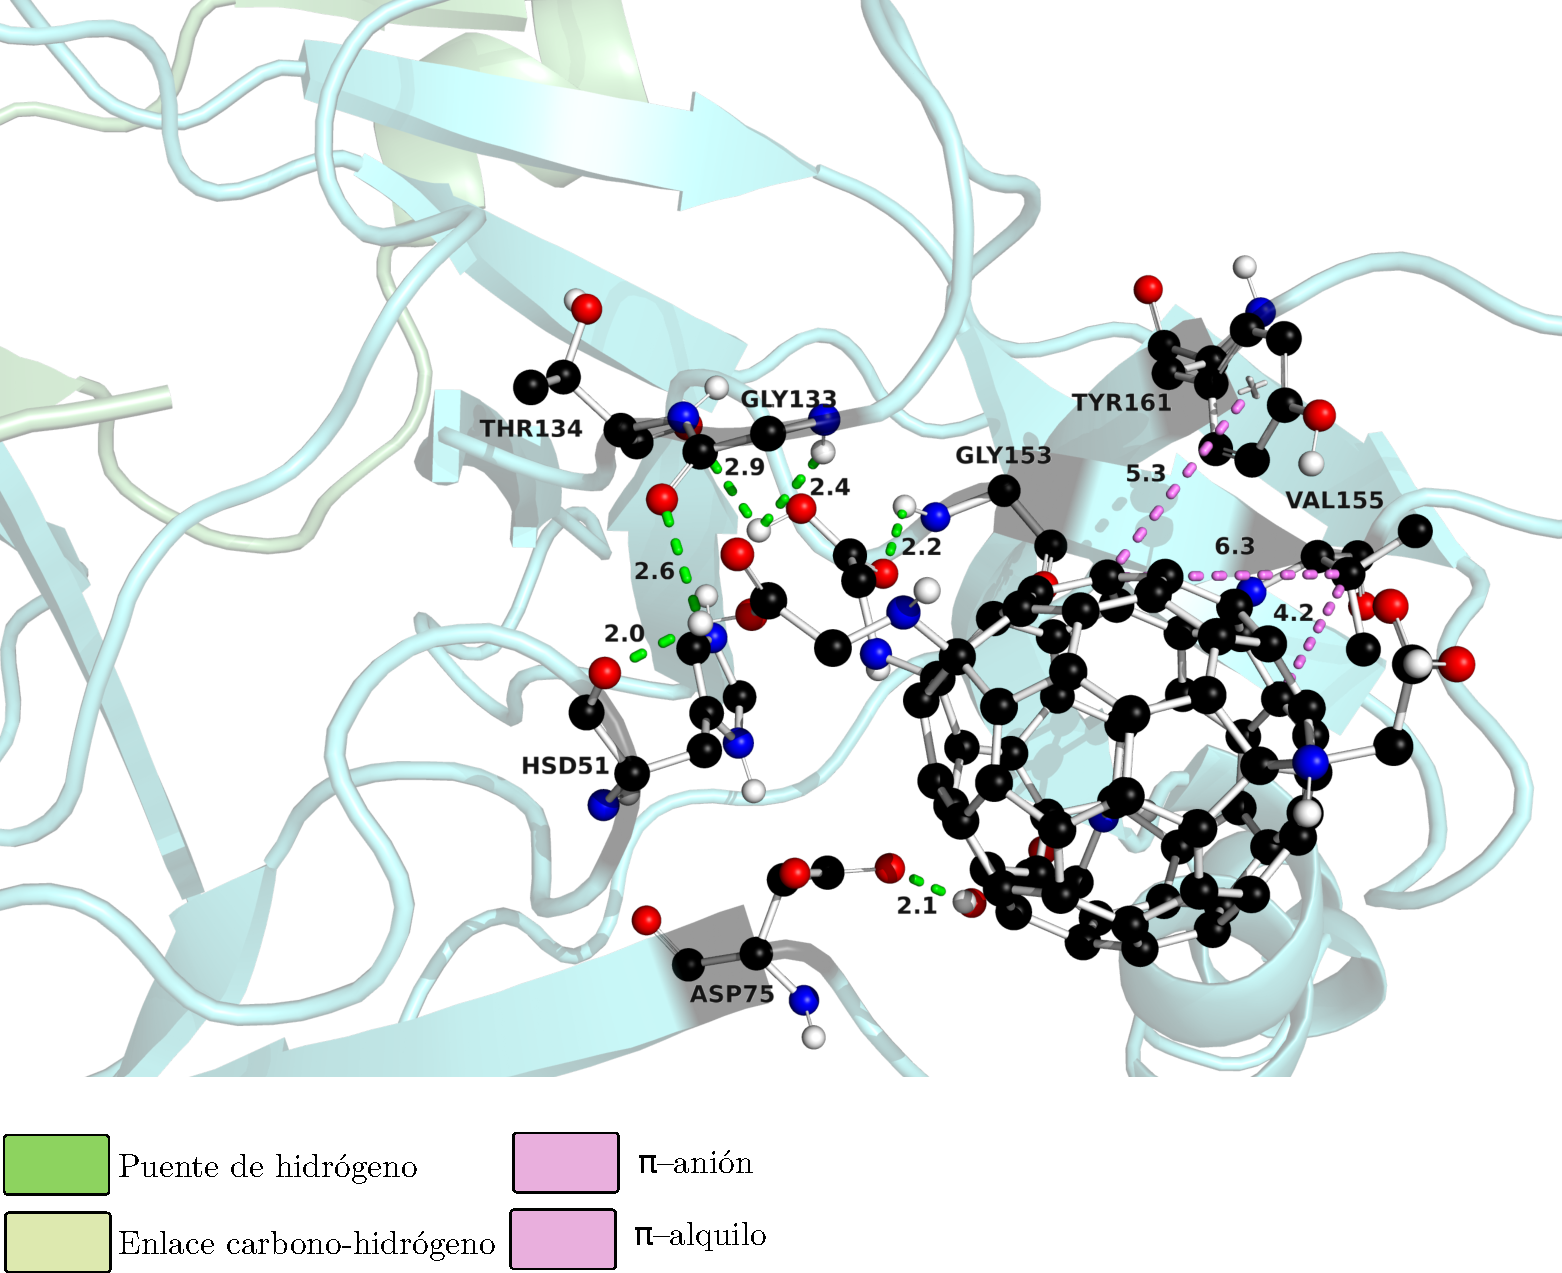
\includegraphics[width=1.0\textwidth]{imagenes/Resu/orto-1.pdf}
      \caption{M.}
      \label{fig:mep-gly4}
        \end{figure}

\begin{figure}[H]
      \centering
      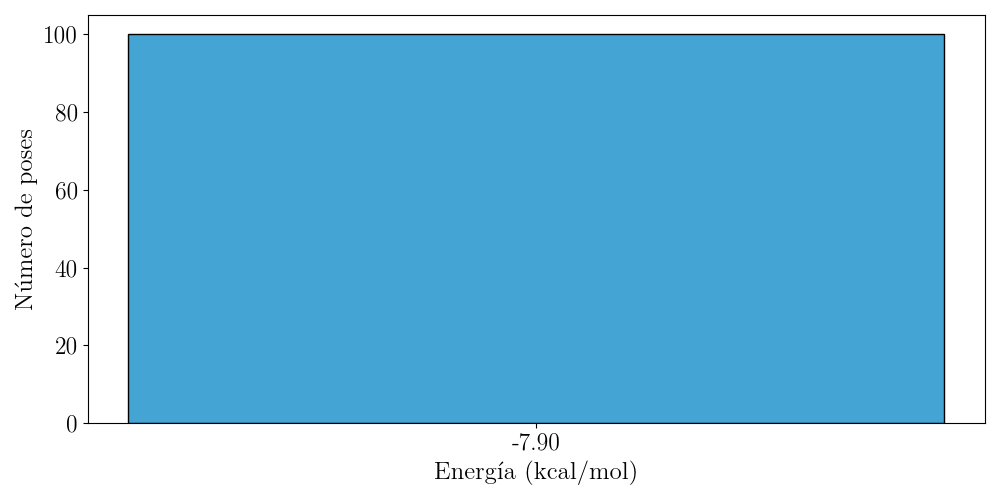
\includegraphics[width=1.0\textwidth]{imagenes/Resu/orto-c60.png}
      \caption{M.}
      \label{fig:mep-gly4}
        \end{figure}


\begin{table}[H]
    \centering
    \footnotesize
    \setlength{\tabcolsep}{5pt}
    \renewcommand{\arraystretch}{1.2}
    \caption{Interacciones no covalentes y distancias de contacto para el acoplamiento del derivado de fullereno C\textsubscript{60}(Gly)\textsubscript{4} orto-c60 en la proteasa de DENV-2 (PDB: 2FOM, Pose 1).}
    \label{tab:interacciones-pose1}
    \begin{tabular}{llcll}
        \toprule
        \multicolumn{1}{c}{\textbf{\shortstack[c]{Tipo de\\interacción}}} & 
        \multicolumn{1}{c}{\textbf{Residuo}} & 
        \multicolumn{1}{c}{\textbf{\shortstack[c]{Distancia\\(\AA)}}} & 
        \multicolumn{1}{c}{\textbf{\shortstack[c]{Motivo\\estructural}}} & 
        \multicolumn{1}{c}{\textbf{\shortstack[c]{Tipo de\\aminoácido}}} \\
        \midrule
        Puente de hidrógeno & Hsd51  & 2.05 & Tríada catalítica & Polar, cargado positivo \\
                            & Asp75  & 2.83 & Tríada catalítica & Polar, cargado negativo \\
                            & Gly133 & 2.07 & Hueco oxianiónico & Apolar / Neutro \\
                            & Thr134 & 2.63 & Sitio de unión & Polar no cargado \\
                            & Gly153 & 2.15 & Sitio de unión & Apolar / Neutro \\
        \midrule
        Interacción hidrofóbica & Val155 & 4.02 & Bolsillo hidrofóbico & Apolar / Hidrofóbico \\
        (Alquil / $\pi$-Alquil) & Tyr161 & 4.72 & Bolsillo hidrofóbico & Polar neutro / Aromático \\
                                & Tyr161 & 5.24 & Bolsillo hidrofóbico & Polar neutro / Aromático \\
        \bottomrule
    \end{tabular}
\end{table}
\subsection{Perfil Energético y Convergencia Absoluta en el Sitio Ortostérico}

El análisis del acoplamiento molecular dirigido al sitio activo ortostérico de la proteasa NS2B/NS3 del serotipo 2 del virus del dengue (PDB ID: \textbf{2FOM}) demostró una afinidad termodinámica excepcional y un patrón de reconocimiento molecular altamente específico para el aducto C\textsubscript{60}(Gly)\textsubscript{4}. A partir de una muestra de 100 poses generadas mediante AutoDock Vina (exhaustividad de 80), el perfil energético (Figura~9.20) exhibió un comportamiento conformacional extraordinario: el 100\% de las poses generadas convergieron en un único conglomerado energéticamente homogéneo con una energía libre de unión ($\Delta G$) de $-7.90\ \text{kcal/mol}$.

Esta convergencia poblacional del 100\% representa un pozo de energía potencial único y profundamente estable dentro del sitio catalítico, eliminando cualquier ambigüedad conformacional. La selección del modo de unión óptimo recayó en la \texttt{pose01.pdb} (Pose 1), la cual ejemplifica el estado en equilibrio dominante y termodinómicamente favorecido en la cavidad ortostérica.

\subsection{Análisis de Contactos No Covalentes e Interacciones Clave}

La caracterización tridimensional de las interacciones no covalentes efectuada en PyMOL y Discovery Studio Visualizer (Tabla~9.9 e Ilustración visual) permitió dilucidar la red de contactos que estabilizan el complejo nanoestructura-proteína en la \texttt{pose01.pdb}:

\begin{itemize}
    \item \textbf{Puentes de hidrógeno convencionales y anclaje catalítico:} Se identificó una densa red de puentes de hidrógeno de corta distancia ($\le 2.83\ \text{\AA}$) coordinados por las cadenas laterales del tetra-aducto de glicina:
    \begin{itemize}
        \item Interacción directa con los residuos de la tríada catalítica \textbf{Hsd51} ($2.05\ \text{\AA}$) y \textbf{Asp75} ($2.83\ \text{\AA}$), bloqueando los centros nucleofílico y de transferencia protónica de la enzima.
        \item Formación de un puente de hidrógeno fuerte con el residuo \textbf{Gly133} ($2.07\ \text{\AA}$), perteneciente al \textit{hueco oxianiónico} (\textit{oxyanion hole}), un elemento estructural crítico involucrado en la estabilización del estado de transición durante la catálisis peptídica.
        \item Contactos polares adicionales con \textbf{Gly153} ($2.15\ \text{\AA}$) y \textbf{Thr134} ($2.63\ \text{\AA}$), reforzando el posicionamiento del ligando en el contorno del sitio activo.
    \end{itemize}
    
    \item \textbf{Interacciones hidrofóbicas en el bolsillo ortostérico ($\text{Alquil} / \pi\text{-Alquil}$):} La esfera de fulereno se acomoda holgadamente en la cavidad apolar mediante interacciones de tipo $\pi$-alquilo con el residuo hidrofóbico \textbf{Val155} ($4.02\ \text{\AA}$) y contactos aromáticos dobles con la cadena lateral de \textbf{Tyr161} a distancias de $4.72\ \text{\AA}$ y $5.24\ \text{\AA}$.
\end{itemize}

\subsection{Contraste Comparativo con el Inhibidor Sintético de Referencia (246DA)}

Al comparar el desempeño del C\textsubscript{60}(Gly)\textsubscript{4} en este sitio ortostérico con el inhibidor sintético de referencia reportado en la literatura, el compuesto 246DA ($K_i = 19.84\ \mu\text{M}$ en PDB ID: \textbf{2FOM}), se identifican ventajas estructurales y bioenergéticas de gran relevancia:

\begin{enumerate}
    \item \textbf{Superioridad Energética e Incremento de Afinidad:} El aducto C\textsubscript{60}(Gly)\textsubscript{4} alcanza una energía de unión de $-7.90\ \text{kcal/mol}$, superando notoriamente la afinidad calculada para el compuesto 246DA ($-5.80\ \text{a}\ -6.00\ \text{kcal/mol}$). Esto representa una ganancia termodinámica de $\Delta\Delta G \approx -1.90\ \text{kcal/mol}$ a favorecer del derivado de fulereno, atribuible a la capacidad del núcleo de C\textsubscript{60}(Gly) de maximizar la superficie de contacto hidrofóbica en combinación con los cuatro brazos polares de glicina.
    
    \item \textbf{Conservación y Ampliación del Farmacóforo Catalítico:} Mientras que el inhibidor 246DA interactúa convencionalmente con la tríada catalítica (\textbf{His51}, \textbf{Asp75} y \textbf{Ser135}), el C\textsubscript{60}(Gly)\textsubscript{4} no solo preserva el anclaje directo con \textbf{Hsd51} ($2.05\ \text{\AA}$) y \textbf{Asp75} ($2.83\ \text{\AA}$), sino que además se ancla directamente al hueco oxianiónico (\textbf{Gly133}, $2.07\ \text{\AA}$). La oclusión simultánea de la tríada catalítica y del hueco oxianiónico sugiere un mecanismo de inhibición competitiva sumamente efectivo que previene el acceso de cualquier sustrato proteico.
    
    \item \textbf{Acomodación en el Bolsillo Lipofílico:} En lugar de la coordinación periférica observada en 246DA con residuos como \textbf{Leu76} o \textbf{Ile165}, el C\textsubscript{60}(Gly)\textsubscript{4} establece un empaquetamiento hidrofóbico optimizado mediante interacciones $\pi$-alquilo con \textbf{Val155} y \textbf{Tyr161}, validando la complementariedad volumétrica entre la cavidad y la nanoestructura esférica.
\end{enumerate}

La convergencia absoluta de las 100 poses en $-7.90\ \text{kcal/mol}$, sumada al bloqueo simultáneo de la tríada catalítica (\textbf{Hsd51}/\textbf{Asp75}) y del hueco oxianiónico (\textbf{Gly133}) a distancias $\le 2.07\ \text{\AA}$, demuestra que el derivado C\textsubscript{60}(Gly)\textsubscript{4} en la \texttt{pose01.pdb} actúa como un candidato inhibidor competitivo ortostérico de alta potencia, superando los parámetros termodinámicos del fármaco de referencia 246DA contra la proteasa del dengue serotipo 2.















\titleformat{\chapter}[display]
  {\normalfont\bfseries}{}{0pt}{\Large} % Este comando es para eliminar la aparición de "Capítulo N" en el PDF. Para emplear el formato de la tesis simplemente eliminamos la línea. 
\chapter{Cronograma}
El trabajo de doctorado se organiza de acuerdo con el cronograma de la Figura~\ref{c:1}. En primer lugar, se propone validar las simulaciones de dinámica molecular con los campos de fuerza utilizados en moléculas orgánicas. Luego se pretende calcular la estructura electrónica de los complejos para obtener el de menor energía. Con ello es posible calcular una serie de descriptores cinéticos y realizar un análisis de interacciones por medio de módulos especiales de GROMACS.
\begin{figure}[h]
    \centering
    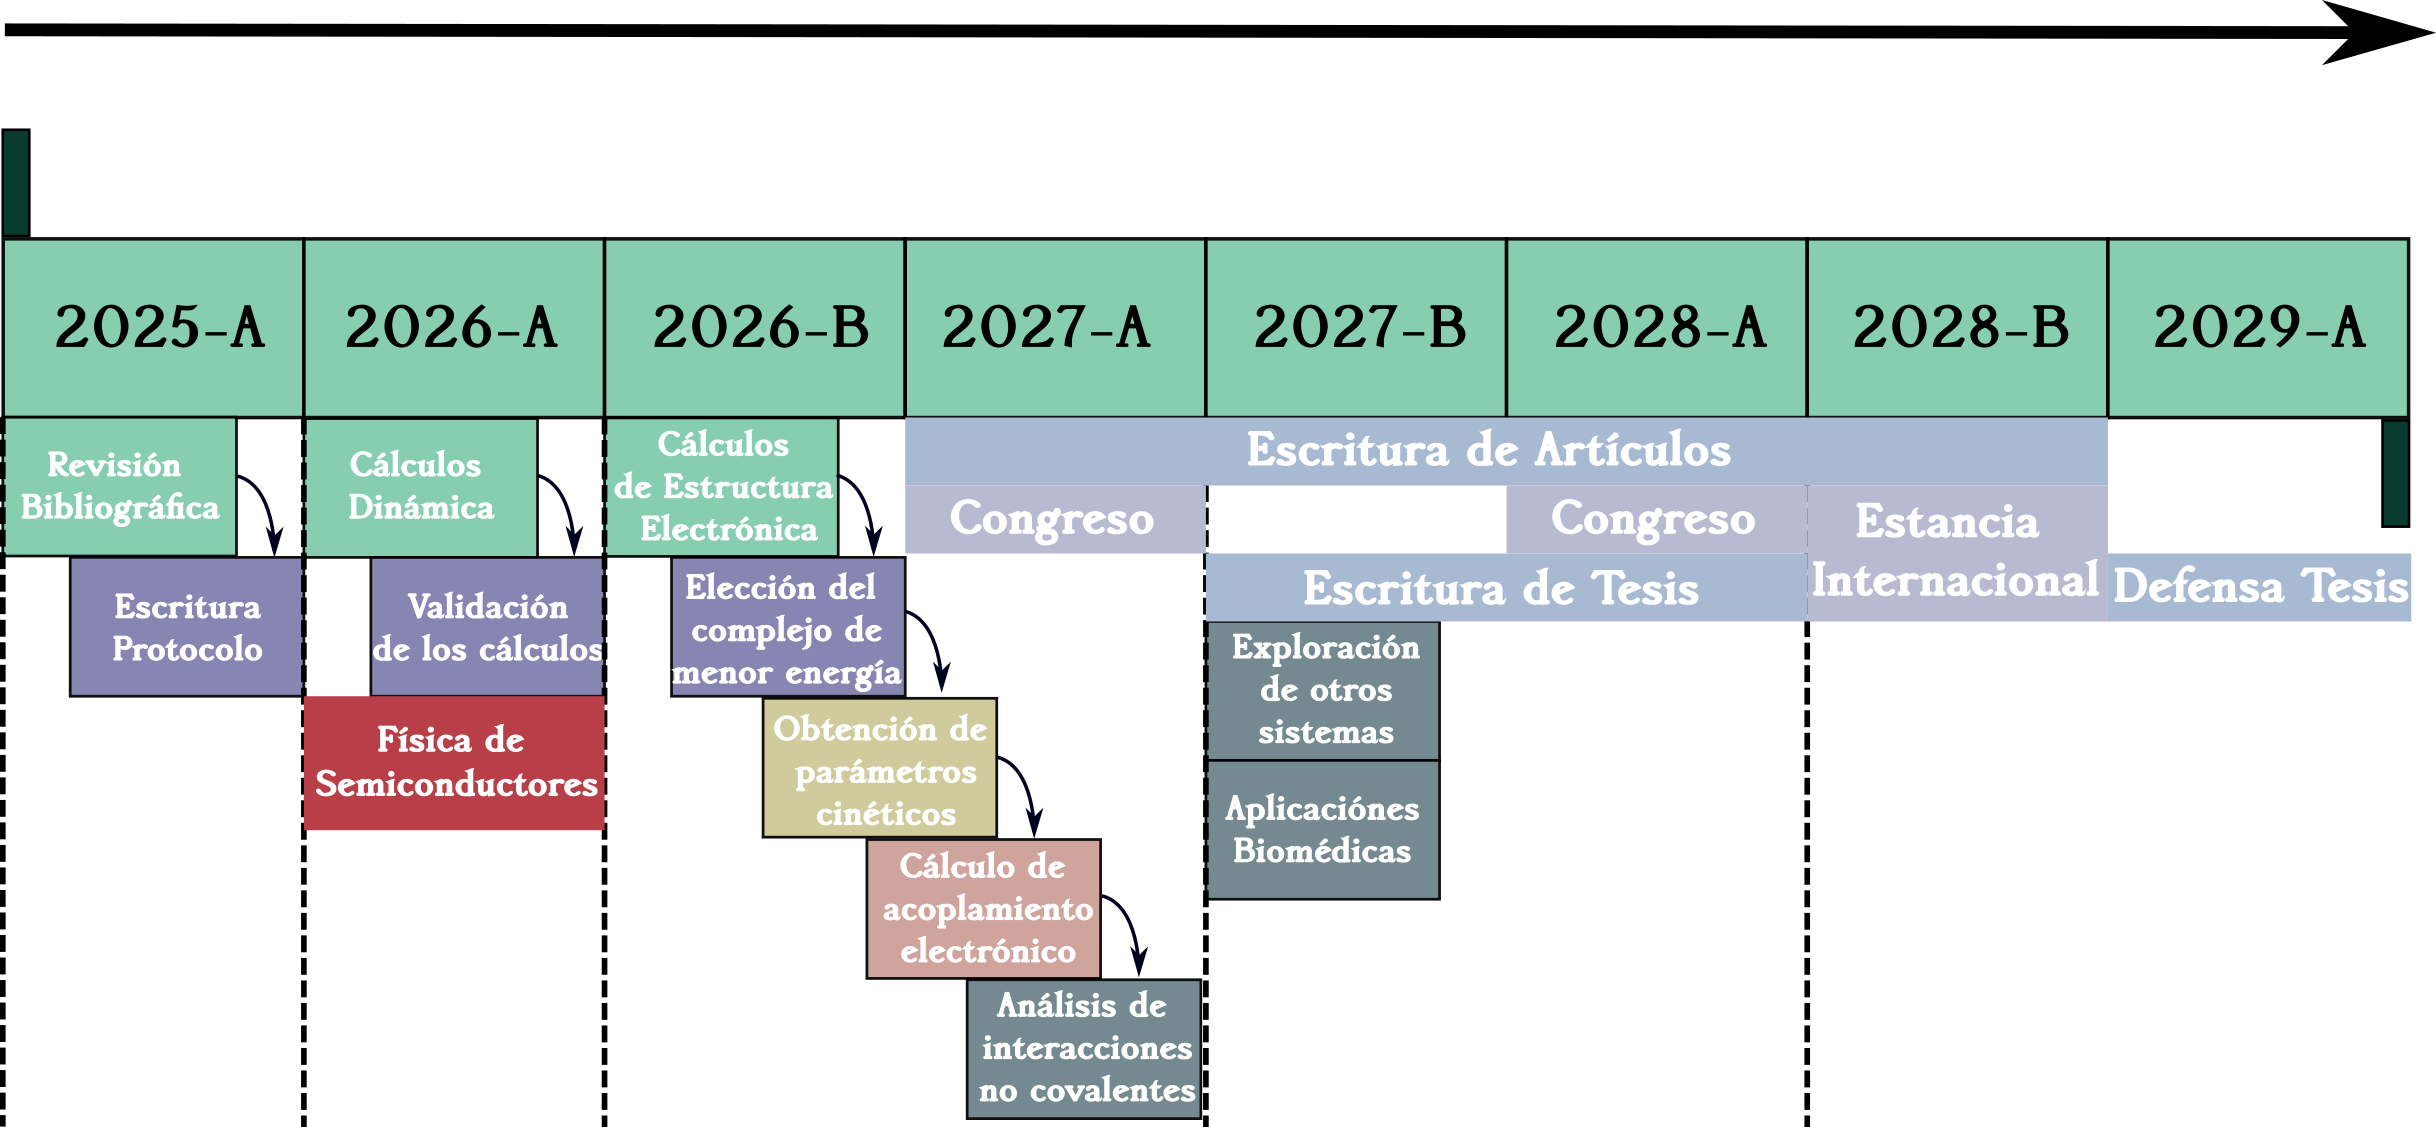
\includegraphics[width=1\textwidth,height=0.5\textwidth]{imagenes/Ant/cro.png}
   \caption{Cronograma de actividades}
    \label{c:1} %Esto genera un numero a mi etiqueta
\end{figure} \\
Finalmente, se contempla redactar dos artículos para su publicación a finales de 2027 o mediados de 2028. También se prevé la participación en dos congresos y una estancia internacional para fortalecer la formación y el conocimiento adquirido durante el doctorado. 
%\titleformat{\chapter}[display]
  {\normalfont\bfseries}{}{0pt}{\Large} % Este comando es para eliminar la aparición de "Capítulo N" en el PDF. Para emplear el formato de la tesis simplemente eliminamos la línea. 
\chapter{Resultados 2025B}
\section{Sistema BTP-4F-XXXX} 
El sistema BTP-4F-XXXX se encuentra conformado por un grupo de siete moléculas: i) BTP-4F-T2C8, ii) BTP-4F-T2EH, iii) BTP-4F-T3EH, iv) BTP-4F-AC8, v) BTP-4F-A2EH, vi) BTP-4F-A3EH y vii) BTP-4F-NC (véase la Figura \ref{R25B:1}). 
\begin{figure}[h]
    \centering
    \includegraphics[width=1\textwidth,height=0.8\textwidth]{~/Documentos/Protocolo-Doctorado/imagenes/R25B/sistema.png}
   \caption{Estructuras químicas del sistema BTP-4F-XXXX}
    \label{R25B:1} %Esto genera un numero a mi etiqueta
\end{figure} \newpage \noindent
Los primeros tres aceptores pertenecen al sistema isomérico estudiado por el grupo de Hu et. al \cite{shang2022over}, mientras que los últimos cuatro han sido propuestos de manera teórica para comparar, caracterizar y detectar cuál es el efecto que las cadenas laterales alquílicas tienen sobre el sistema BTP-4F-XXXX. Para ello, primero se obtuvieron las geometrías optimizadas de cada aceptor empleando para ello la DFT \cite{kohn1965self} con el funcional de intercambio y correlación HSE06 \cite{heyd2004efficient} con el conjunto base 6-311++g(d,p), añadiendo el modelo del continuum polarizable PCM \cite{cossi1996ab} para incluir los efectos de solvatación del cloroformo. El empleo de esta metodología se encuentra respaldada en trabajos previos \cite{chico2024study, romo2022improvement} y es una elección adecuada para este sistema debido a la precisión alta con la que se describen las energías del LUMO caracterizadas de forma experimental para el sistema T2C8, T2EH y T3EH. Además, la inclusión de funciones difusas permite describir de mejor manera a electrones que se encuentran ligados débilmente al núcleo. Estos cálculos fueron ejecutados con el paquete de software \textit{GAUSSIAN 16}.  \cite{frisch2016gaussian}. 
\section{Espectros UV-vis}
Se exploraron 50 estados electrónicos excitados para cada aceptor implementando un cálculo de energía TD-SCF \cite{makri1987time} con la misma metodología HSE06/6-311++g(d,p) bajo condiciones de solvatación en cloroformo usando el modelo PCM. Los espectros normalizados de los siete aceptores se pueden ver en la Figura \ref{R25B:2}.
\begin{figure}[h]
    \centering
    \includegraphics[width=0.8\textwidth,height=0.55\textwidth]{~/Documentos/Protocolo-Doctorado/imagenes/R25B/spectralall.png}
   \caption{Conjunto de espectos Uv-vis del sistema BTP-4F-XXXX}
    \label{R25B:2} %Esto genera un numero a mi etiqueta
\end{figure} \\
Es apreciable la presencia de un pico máximo principal y la de otros dos picos secundarios. En la Tabla \ref{table:R25B-1} se muestra la caracterización de estos picos formados por transiciones hacia al primer estado excitado de cada aceptor, los cuáles están acompañados de su respectiva fuerza del oscilador $f$. Los picos máximos ($\lambda_{max}$) ordenados de mayor a menor van en: A3EH>T3EH>NC>(AC8, A2EH)>(T2C8, T2EH). Esta tendencia nos sugiere dos puntos principales: i) el par de aceptores (T2C8, T2EH) presentan una $\lambda_{max}$ equivalente; este patrón es observable aún cuando se ha sustraído una de las cadenas alquílicas del anillo de tiofeno, tal como se ve en los valores de $\lambda_{max}$ del par (AC8, A2EH).  \newpage
\noindent Aunado al punto anterior, la forma de curva del espectro del par (T2C8, T2EH) se encuentra en su mayoría superpuesta una sobre la otra teniendo ligeros desplazamientos en los picos secundarios. Por otra parte, ii) los espectros de los aceptores sustituidos con cadenas alquílicas en la posición $\beta$ del anillo de tiofeno: T3EH, A3EH presentan un perfil óptico muy diferente. 
\begin{table}[h] %La h es para decirle que coloque la tabla con el texto
\caption{Perfil óptico del espectro de absorción UV-vis del sistema BPT-4F-XXXX }
\label{table:R25B-1} \vspace{-0.5cm}
\begin{center} 
\begin{tabular}{ccc}
\hline
Aceptor & $\lambda_{max}$ (nm) & Fuerza del Oscilador $f$ \\ \hline
BTP-4F-T2C8 & 739.64 & 2.0115 \\
BTP-4F-T2EH & 739.64 & 1.9976 \\
BTP-4F-T3EH & 746.10 & 2.0370 \\
BTP-4F-AC8 & 742.04 & 2.0043 \\
BTP-4F-A2EH & 742.04 & 1.9925 \\
BTP-4F-A3EH & 746.85 & 2.0499 \\
BTP-4F-NC & 743.24 & 2.0183  \\ \hline
\end{tabular}
\end{center}
\vspace{-0.2cm}
\end{table} \\ 
Las $\lambda_{max}$ de este par de aceptores presentan un mayor desplazamiento batocrómico con respecto a los demás. Sumado a esto, el aceptor BTP-4F-NC tiene un mayor corrimiento al rojo con respecto al par (T2EH, T2C8) incluso cuando no tiene cadenas alquílicas sustituidas sobre sus anillos de tiofeno. Esta tendencia sugiere que el comportamiento óptico del sistema esta mayormente influenciado por cambios en la posición del anillo y la asimetría del sistema presente sobre las cadenas hidrocarbonadas. Por otra parte, los picos secundarios muestran un conjunto de desplazamientos únicos. Estos cambios son regidos por un perfil óptico variable, al menos en el rango donde estos picos están localizados. Para explicar más a detalle esta última premisa, en la Tabla \ref{table:R25B-2} se muestran las bandas de mayor $f$ ubicadas entre 300-400 nm (banda A) y 500-600 nm (banda B) de cada aceptor y la máxima de la envolvente gaussiana. 
\begin{table}[h] %La h es para decirle que coloque la tabla con el texto
\caption{Perfil óptico del espectro de absorción UV-vis del sistema BPT-4F-XXXX }
\label{table:R25B-2} \vspace{-0.5cm}
\begin{center} 
\begin{tabular}{ccccccc}
\hline 
Aceptor & Banda A (nm) & $f$ & $\lambda_{max}^A $ (nm) & Banda B (nm) & $f$ & $\lambda_{max}^B $ (nm)  \\ \hline \
BTP-4F-T2C8 & 352.91 &  0.2151 & 356.48 & 520.56 & 0.3978 & 538.17  \\
BTP-4F-T2EH &  352.96 & 0.2218 & 356.48 & 520.95 &  0.4156 & 540.97 \\
BTP-4F-T3EH & 352.83 & 0.2145 & 357.28 & 521.33 & 0.4276 & 532.97 \\
BTP-4F-AC8 & 360.78 & 0.1210 & 354.88 & 517.18 & 0.4519 & 525.36  \\
BTP-4F-A2EH & 352.28 & 0.1476 & 354.88 &517.09 &  0.4720 & 524.96\\
BTP-4F-A3EH & 352.55 & 0.2008 & 355.28 & 518.15 &  0.4526 & 525.76\\
BTP-4F-NC & 351.80 &  0.2059 &353.28 & 517.78 & 0.3934 & 520.56 \\ \hline
\end{tabular}
\end{center}
\vspace{-0.2cm}
\end{table} \\
En la Figura \ref{R25B:3} se presentan los espectros UV-vis del conjunto de siete aceptores sin normalizar. Las intensidades de las $\lambda_{max}$ de cada aceptor varían de acuerdo con la siguiente tendencia: A3EH>T3EH>NC>T2C8>AC8>T2EH>A2EH, este patrón era esperado al observarse el mismo incremento en los valores de la fuerza del oscilador $f$. Por otro lado, los valores del $f$ localizados en la banda A van de acuerdo con el siguiente orden: T2EH>T2C8>T3EH>NC>A3EH>A2EH>AC8. Sin embargo, la contribución de otros estados excitados adyacentes, propicia que las intensidades de los picos formados en la zona A del espectro de la Figura \ref{R25B:3}, vayan en el siguiente acomodo: NC>AC8>A2EH>T2C8>T2EH>A3EH>T3EH. Dentro de este rango, es notable que hay un mayor desplazamiento hacia el azul del pico secundario A del BTP-4F-NC, véase la Figura \ref{R25B:4}. Cabe señalar que este corrimiento también es observado en el pico de la zona B y el orden de las intensidades de los picos localizados en dicha zona van en aumento de acuerdo con el siguiente arreglo: NC>A3EH>(AC8, T3EH, T2EH, T2C8)>A2EH. \newpage \noindent
\vspace{-1cm}
\begin{figure}[h]
    \centering
    \includegraphics[width=0.8\textwidth,height=0.55\textwidth]{~/Documentos/Protocolo-Doctorado/imagenes/R25B/spectralall-f.png}
   \caption{Conjunto de espectos Uv-vis del sistema BTP-4F-XXXX sin normalizar}
    \label{R25B:3} %Esto genera un numero a mi etiqueta
\end{figure} \\
La relevancia de estos picos secundarios subyace en cómo las cadenas alquílicas son capaces de modular el perfil óptico de los aceptores. En principio, los mayores desplazamientos hacia al azul se observan a medida que se las cadenas hidrocarbonadas se van retirando del anillo de tiofeno, al menos para los picos situados en la zona B del espectro. No obstante, en regiones más cercanas al ultravioleta los desplazamientos de $\lambda_{max}^A$ son mayormente influenciados por la sustitución de la cadena alquílica en el carbono $\beta$ del anillo de tiofeno.  
\begin{figure}[h]
    \centering
    \includegraphics[width=0.5\textwidth,height=0.35\textwidth]{~/Documentos/Protocolo-Doctorado/imagenes/R25B/secondpiks.png}
   \caption{Desplazamientos hipsocrómicos de los picos secundarios A y B de los espectos Uv-vis del sistema BTP-4F-XXXX}
    \label{R25B:4} %Esto genera un numero a mi etiqueta
\end{figure} \\
Para obtener mayor información de las configuraciones correspondientes de cada estado excitado, en las Tablas \ref{table:R25B-3}, \ref{table:R25B-4}, \ref{table:R25B-5} \ref{table:R25B-6}, \ref{table:R25B-7}, \ref{table:R25B-8} y \ref{table:R25B-9}, se presentan los NTOs (\textit{Natural Transition Orbitals}) de cada aceptor, de los cuales solo se muestran las configuraciones con una aportación mayor al 10\% de la transición correspondiente.  
\begin{table}[H] %La h es para decirle que coloque la tabla con el texto
\caption{NTOs del aceptor BTP-4F-T2C8}
\label{table:R25B-3} \vspace{-0.5cm}
{\footnotesize
\begin{center} 
\begin{tabular}{ccccc}
\hline
EE & Energía (eV) & $f$ & $\lambda$ (nm) & Configuración \\ \hline
1 & 1.67 & 2.0115 & 739.94 &  H$\rightarrow$L 99\% \\ 
2 & 1.95 & 0.1084 & 635.27  & H$\rightarrow$L 93\% \\ 
3 & 2.16 & 0.3182 & 573.78 & H$\rightarrow$L 92\% \\
4 & 2.25 & 0.2364 & 550.22 & H$\rightarrow$L 58\%, H-1$\rightarrow$L+1 41\% \\  
5 & 2.28 & 0.0072 & 543.54 &H$\rightarrow$L 59\%, H-1$\rightarrow$L+1 41\% \\
6 &  2.31 & 0.0119 & 536.34 & H$\rightarrow$L 75\%, H-1$\rightarrow$L+1 24\% \\
7 & 2.38 & 0.0343 & 520.76 & H$\rightarrow$L 93\% \\ 
8 & 2.38 & 0.3978 & 520.56 & H$\rightarrow$L 70\%, H-1$\rightarrow$L+1 25\% \\ 
9 & 2.51 & 0.0723 & 493.87 & H$\rightarrow$L 98\% \\ 
10 & 2.52 & 0.0787 & 491.75 & H$\rightarrow$L 98\% \\ 
11 & 2.65 & 0.0021 & 467.56 & H$\rightarrow$L 97\% \\ 
12 & 2.74 & 0.0391 & 451.41 & H$\rightarrow$L 73\%, H-1$\rightarrow$L+1 24\% \\
13 & 2.74 & 0.0715 & 451.28 & H$\rightarrow$L 70\%, H-1$\rightarrow$L+1 24\% \\
14 & 2.77 & 0.0505 & 447.46 & H$\rightarrow$L 90\% \\
15 & 2.83 & 0.0290 & 437 & H$\rightarrow$L 89\% \\
16 & 2.87 & 0.0374 & 430.77 & H$\rightarrow$L 98\% \\ 
17 & 2.91 & 0.0258 & 424.79 & H$\rightarrow$L 90\% \\ 
18 & 2.93 & 0.0076 & 421.80 &  H$\rightarrow$L 95\%  \\ 
19 & 2.98 & 0.0038 & 415.67 & H$\rightarrow$L 82\%, H-1$\rightarrow$L+1 15\% \\ 
20 & 2.99 & 0.0089 & 414.06 &  H$\rightarrow$L 77\%, H-1$\rightarrow$L+1 19\% \\ 
21 & 3.01 & 410.84 & 0.0716 & H$\rightarrow$L 60\%, H-1$\rightarrow$L+1 35\% \\ 
22 & 3.15 & 0.0309 & 393.18 & H$\rightarrow$L 93\% \\ 
23 & 3.18 & 0.0317 & 388.86 & H$\rightarrow$L 94\% \\ 
24 & 3.21 & 0.0006 & 385.98 & H$\rightarrow$L 93\% \\ 
25 & 3.25 & 0.0227 & 380.87 & H$\rightarrow$L 81\% \\ 
26 & 3.27 & 0.0446 & 378.43 & H$\rightarrow$L 90\% \\ 
27 & 3.29 & 0.0128 & 376.69 & H$\rightarrow$L 79\%, H-1$\rightarrow$L+1 12\% \\ 
28 & 3.30 & 0.0010 & 375.37 & H$\rightarrow$L 91\% \\ 
29 & 3.34 & 0.0401 & 371.11 &  H$\rightarrow$L 38\%, H-1$\rightarrow$L+1 26\%, H-2$\rightarrow$L+2 16\%, H-3$\rightarrow$L+3 14\% \\
30 & 3.35 & 0.0009 & 369.16 & H$\rightarrow$L 80\% \\ 
31 & 3.38 & 0.0176 & 366.77 &  H$\rightarrow$L 75\%, H-1$\rightarrow$L+1 21\% \\
32 & 3.39 & 0.0035 & 364.86 &   H$\rightarrow$L 66\%, H-1$\rightarrow$L+1 19\% \\ 
33 & 3.42 & 0.1517 & 362.02 &  H$\rightarrow$L 64\%, H-1$\rightarrow$L+1 15\%,  H-2$\rightarrow$L+2 14\% \\ 
34 & 3.42 & 0.0206 & 361.73 &  H$\rightarrow$L 94\% \\
35 & 3.45 & 0.0071 & 358.44 &  H$\rightarrow$L 59\%, H-1$\rightarrow$L+1 20\%, H-2$\rightarrow$L+2 11\% \\ 
36 & 3.46 & 0.0133 & 358.07 &  H$\rightarrow$L 83\% \\ 
37 & 3.47 & 0.1047 & 356.38 &  H$\rightarrow$L 35\%, H-1$\rightarrow$L+1 32\%,  H-2$\rightarrow$L+2 19\%, H-3$\rightarrow$L+3 13\% \\ 
38 & 3.50 & 0.0227 & 353.98 &  H$\rightarrow$L 81\% \\
39 &  3.51 & 0.2151 & 351.91 &  H$\rightarrow$L 95\% \\ 
40 & 3.51 & 0.0031 & 352.47 &  H$\rightarrow$L 73\%, H-1$\rightarrow$L+1 15\% \\ 
41 & 3.53 & 0.0086 & 350.84 &  H$\rightarrow$L 66\%, H-1$\rightarrow$L+1 16\%,  H-2$\rightarrow$L+2 13\% \\
42 & 3.54 & 0.0385 & 349.52 &   H$\rightarrow$L 45\%, H-1$\rightarrow$L+1 31\%,  H-2$\rightarrow$L+2 18\% \\ 
43 & 3.55 & 0.0024 & 348.64 &  H$\rightarrow$L 41\%, H-1$\rightarrow$L+1 38\% \\ 
44 & 3.58 & 0.0005 & 346.28 &  H$\rightarrow$L 38\%, H-1$\rightarrow$L+1 28\%,  H-2$\rightarrow$L+2 12\%,  H-3$\rightarrow$L+3 10\%, H-4$\rightarrow$L+4 10\% \\
45 &  3.60 & 0.0649 & 343.76 &  H$\rightarrow$L 51\%, H-1$\rightarrow$L+1 43\% \\ 
46 & 3..64 & 0.0186 & 339.69 &  H$\rightarrow$L 51\%, H-1$\rightarrow$L+1 37\% \\ 
47 & 3.78 & 0.0374 & 327.39 &  H$\rightarrow$L 91\% \\ 
48 & 3.84 & 0.1101 & 322.82 &  H$\rightarrow$L 56\%, H-1$\rightarrow$L+1 32\% \\ 
49 & 3.84 & 0.1585 & 322.27 &  H$\rightarrow$L 52\%, H-1$\rightarrow$L+1 23\%,  H-2$\rightarrow$L+2 15\% \\
50 & 3.85 & 0.0144 & 321.78 &  H$\rightarrow$L 36\%, H-1$\rightarrow$L+1 29\%,  H-2$\rightarrow$L+2 16\%, H-3$\rightarrow$L+3 11\% \\ \hline
\end{tabular} 
\end{center} }
\vspace{-0.2cm}
\end{table} \newpage \noindent

\begin{table}[H]
\caption{NTOs del aceptor BTP-4F-T2EH}
\label{table:R25B-4} \vspace{-0.5cm}
{\footnotesize
\begin{center} 
\begin{tabular}{ccccc}
\hline
EE & Energía (eV) & $f$ & $\lambda$ (nm) & Configuración \\ \hline
1 & 1.68 & 1.9976 & 739.87 & H $\rightarrow$ L 100\% \\
2 & 1.95 & 0.1062 & 635.31 & H $\rightarrow$ L 93\% \\
3 & 2.15 & 0.3536 & 576.80 & H $\rightarrow$ L 93\% \\
4 & 2.25 & 0.2275 & 552.25 & H $\rightarrow$ L 66\%, H-1 $\rightarrow$ L+1 33\% \\
5 & 2.27 & 0.0100 & 545.08 & H $\rightarrow$ L 66\%, H-1 $\rightarrow$ L+1 33\% \\
6 & 2.31 & 0.0120 & 536.38 & H $\rightarrow$ L 76\%, H-1 $\rightarrow$ L+1 23\% \\
7 & 2.37 & 0.0211 & 523.42 & H $\rightarrow$ L 98\% \\
8 & 2.38 & 0.4156 & 520.95 & H $\rightarrow$ L 74\%, H-1 $\rightarrow$ L+1 24\% \\
9 & 2.50 & 0.0316 & 495.96 & H $\rightarrow$ L 98\% \\
10 & 2.52 & 0.1252 & 492.48 & H $\rightarrow$ L 98\% \\
11 & 2.65 & 0.0018 & 468.03 & H $\rightarrow$ L 97\% \\
12 & 2.74 & 0.0936 & 452.69 & H $\rightarrow$ L 90\% \\
13 & 2.75 & 0.0227 & 451.54 & H $\rightarrow$ L 96\% \\
14 & 2.76 & 0.0494 & 449.39 & H $\rightarrow$ L 89\% \\
15 & 2.82 & 0.0271 & 438.97 & H $\rightarrow$ L 89\% \\
16 & 2.88 & 0.0389 & 431.20 & H $\rightarrow$ L 98\% \\
17 & 2.90 & 0.0268 & 426.90 & H $\rightarrow$ L 90\% \\
18 & 2.94 & 0.0055 & 421.88 & H $\rightarrow$ L 94\% \\
19 & 2.97 & 0.0101 & 417.13 & H $\rightarrow$ L 89\% \\
20 & 2.99 & 0.0093 & 415.11 & H $\rightarrow$ L 56\%, H-1 $\rightarrow$ L+1 39\% \\
21 & 3.01 & 0.0665 & 411.50 & H $\rightarrow$ L 49\%, H-1 $\rightarrow$ L+1 47\% \\
22 & 3.15 & 0.0301 & 393.70 & H $\rightarrow$ L 93\% \\
23 & 3.21 & 0.0425 & 386.53 & H $\rightarrow$ L 93\% \\
24 & 3.24 & 0.0056 & 383.08 & H $\rightarrow$ L 93\% \\
25 & 3.25 & 0.0020 & 381.28 & H $\rightarrow$ L 87\% \\
26 & 3.28 & 0.0434 & 378.37 & H $\rightarrow$ L 83\% \\
27 & 3.29 & 0.0090 & 377.03 & H $\rightarrow$ L 73\%, H-1 $\rightarrow$ L+1 10\% \\
28 & 3.29 & 0.0014 & 376.70 & H $\rightarrow$ L 83\% \\
29 & 3.34 & 0.0461 & 371.57 & H $\rightarrow$ L 40\%, H-1 $\rightarrow$ L+1 24\%, H-2 $\rightarrow$ L+2 17\%, H-3 $\rightarrow$ L+3 16\% \\
30 & 3.36 & 0.0006 & 369.15 & H $\rightarrow$ L 82\% \\
31 & 3.38 & 0.0190 & 367.19 & H $\rightarrow$ L 74\%, H-1 $\rightarrow$ L+1 22\% \\
32 & 3.39 & 0.0032 & 365.25 & H $\rightarrow$ L 63\%, H-1 $\rightarrow$ L+1 18\% \\
33 & 3.41 & 0.0198 & 363.22 & H $\rightarrow$ L 89\% \\
34 & 3.42 & 0.1541 & 362.34 & H $\rightarrow$ L 65\%, H-1 $\rightarrow$ L+1 15\%, H-2 $\rightarrow$ L+2 14\% \\
35 & 3.46 & 0.0039 & 358.57 & H $\rightarrow$ L 61\%, H-1 $\rightarrow$ L+1 19\%, H-2 $\rightarrow$ L+2 10\% \\
36 & 3.47 & 0.0517 & 357.28 & H $\rightarrow$ L 57\%, H-1 $\rightarrow$ L+1 23\%, H-2 $\rightarrow$ L+2 12\% \\
37 & 3.48 & 0.0645 & 356.09 & H $\rightarrow$ L 37\%, H-1 $\rightarrow$ L+1 27\%, H-2 $\rightarrow$ L+2 19\%, H-3 $\rightarrow$ L+3 15\% \\
38 & 3.51 & 0.2218 & 352.96 & H $\rightarrow$ L 95\% \\
39 & 3.51 & 0.0114 & 352.83 & H $\rightarrow$ L 78\%, H-1 $\rightarrow$ L+1 13\% \\
40 & 3.52 & 0.0179 & 352.41 & H $\rightarrow$ L 66\%, H-1 $\rightarrow$ L+1 24\% \\
41 & 3.54 & 0.0029 & 350.70 & H $\rightarrow$ L 53\%, H-1 $\rightarrow$ L+1 26\%, H-2 $\rightarrow$ L+2 16\% \\
42 & 3.56 & 0.0201 & 348.76 & H $\rightarrow$ L 52\%, H-1 $\rightarrow$ L+1 33\% \\
43 & 3.56 & 0.0049 & 348.20 & H $\rightarrow$ L 48\%, H-1 $\rightarrow$ L+1 33\%, H-2 $\rightarrow$ L+2 12\% \\
44 & 3.58 & 0.0013 & 346.50 & H $\rightarrow$ L 36\%, H-1 $\rightarrow$ L+1 30\%, H-2 $\rightarrow$ L+2 13\%, H-3 $\rightarrow$ L+3 10\% \\
45 & 3.60 & 0.0668 & 343.92 & H $\rightarrow$ L 51\%, H-1 $\rightarrow$ L+1 43\% \\
46 & 3.65 & 0.0224 & 339.91 & H $\rightarrow$ L 50\%, H-1 $\rightarrow$ L+1 37\% \\
47 & 3.78 & 0.0386 & 327.77 & H $\rightarrow$ L 91\% \\
48 & 3.83 & 0.0927 & 323.34 & H $\rightarrow$ L 53\%, H-1 $\rightarrow$ L+1 37\% \\
49 & 3.85 & 0.1154 & 322.27 & H $\rightarrow$ L 50\%, H-1 $\rightarrow$ L+1 24\%, H-2 $\rightarrow$ L+2 11\%, H-3 $\rightarrow$ L+3 11\% \\
50 & 3.85 & 0.0469 & 322.08 & H $\rightarrow$ L 41\%, H-1 $\rightarrow$ L+1 26\%, H-2 $\rightarrow$ L+2 14\%, H-3 $\rightarrow$ L+3 13\% \\
\hline
\end{tabular}
\end{center} }
\vspace{-0.2cm}
\end{table} \newpage \noindent

\begin{table}[H]
\caption{NTOs del aceptor BTP-4F-T3EH}
\label{table:R25B-5} \vspace{-0.5cm}
{\footnotesize
\begin{center} 
\begin{tabular}{ccccc}
\hline
EE & Energía (eV) & $f$ & $\lambda$ (nm) & Configuración \\ \hline
1 & 1.66 & 2.0370 & 746.10 & H $\rightarrow$ L 100\% \\
2 & 1.95 & 0.1154 & 636.99 & H $\rightarrow$ L 93\% \\
3 & 2.18 & 0.2674 & 568.74 & H $\rightarrow$ L 93\% \\
4 & 2.26 & 0.1559 & 548.48 & H $\rightarrow$ L 91\% \\
5 & 2.30 & 0.0184 & 538.47 & H $\rightarrow$ L 73\%, H-1 $\rightarrow$ L+1 26\% \\
6 & 2.31 & 0.0602 & 536.89 & H $\rightarrow$ L 90\% \\
7 & 2.38 & 0.4276 & 521.33 & H $\rightarrow$ L 71\%, H-1 $\rightarrow$ L+1 28\% \\
8 & 2.41 & 0.0123 & 513.96 & H $\rightarrow$ L 98\% \\
9 & 2.51 & 0.1500 & 493.12 & H $\rightarrow$ L 97\% \\
10 & 2.56 & 0.0091 & 484.19 & H $\rightarrow$ L 99\% \\
11 & 2.64 & 0.0018 & 469.21 & H $\rightarrow$ L 97\% \\
12 & 2.73 & 0.0572 & 453.97 & H $\rightarrow$ L 96\% \\
13 & 2.74 & 0.0197 & 452.35 & H $\rightarrow$ L 95\% \\
14 & 2.81 & 0.0661 & 441.14 & H $\rightarrow$ L 96\% \\
15 & 2.88 & 0.0190 & 431.25 & H $\rightarrow$ L 92\% \\
16 & 2.88 & 0.0386 & 430.67 & H $\rightarrow$ L 97\% \\
17 & 2.94 & 0.0060 & 421.19 & H $\rightarrow$ L 95\% \\
18 & 2.97 & 0.0217 & 417.28 & H $\rightarrow$ L 71\%, H-1 $\rightarrow$ L+1 23\% \\
19 & 2.99 & 0.0168 & 414.76 & H $\rightarrow$ L 41\%, H-1 $\rightarrow$ L+1 32\%, H-2 $\rightarrow$ L+2 22\% \\
20 & 3.00 & 0.0005 & 413.90 & H $\rightarrow$ L 97\% \\
21 & 3.01 & 0.0544 & 411.48 & H $\rightarrow$ L 48\%, H-1 $\rightarrow$ L+1 46\% \\
22 & 3.03 & 0.0003 & 409.48 & H $\rightarrow$ L 99\% \\
23 & 3.04 & 0.0040 & 407.34 & H $\rightarrow$ L 97\% \\
24 & 3.15 & 0.0295 & 393.95 & H $\rightarrow$ L 93\% \\
25 & 3.23 & 0.1116 & 383.55 & H $\rightarrow$ L 85\% \\
26 & 3.26 & 0.0086 & 379.82 & H $\rightarrow$ L 60\%, H-1 $\rightarrow$ L+1 38\% \\
27 & 3.29 & 0.0107 & 377.18 & H $\rightarrow$ L 69\%, H-1 $\rightarrow$ L+1 26\% \\
28 & 3.30 & 0.0077 & 375.52 & H $\rightarrow$ L 71\%, H-1 $\rightarrow$ L+1 13\%, H-2 $\rightarrow$ L+2 11\% \\
29 & 3.32 & 0.0019 & 373.29 & H $\rightarrow$ L 56\%, H-1 $\rightarrow$ L+1 32\% \\
30 & 3.33 & 0.0139 & 371.91 & H $\rightarrow$ L 46\%, H-1 $\rightarrow$ L+1 19\%, H-2 $\rightarrow$ L+2 18\%, H-3 $\rightarrow$ L+3 11\% \\
31 & 3.35 & 0.0067 & 370.45 & H $\rightarrow$ L 42\%, H-1 $\rightarrow$ L+1 26\%, H-2 $\rightarrow$ L+2 15\% \\
32 & 3.35 & 0.0043 & 369.95 & H $\rightarrow$ L 72\%, H-1 $\rightarrow$ L+1 14\% \\
33 & 3.38 & 0.0160 & 366.53 & H $\rightarrow$ L 81\%, H-1 $\rightarrow$ L+1 12\% \\
34 & 3.39 & 0.0105 & 365.28 & H $\rightarrow$ L 71\%, H-1 $\rightarrow$ L+1 17\% \\
35 & 3.43 & 0.1219 & 361.77 & H $\rightarrow$ L 42\%, H-1 $\rightarrow$ L+1 29\%, H-2 $\rightarrow$ L+2 23\% \\
36 & 3.45 & 0.0522 & 359.72 & H $\rightarrow$ L 41\%, H-1 $\rightarrow$ L+1 40\%, H-2 $\rightarrow$ L+2 11\% \\
37 & 3.46 & 0.0993 & 357.90 & H $\rightarrow$ L 32\%, H-1 $\rightarrow$ L+1 31\%, H-2 $\rightarrow$ L+2 24\% \\
38 & 3.47 & 0.0096 & 356.95 & H $\rightarrow$ L 96\% \\
39 & 3.51 & 0.0140 & 353.08 & H $\rightarrow$ L 72\%, H-1 $\rightarrow$ L+1 10\% \\
40 & 3.51 & 0.2145 & 352.83 & H $\rightarrow$ L 94\% \\
41 & 3.53 & 0.0030 & 351.52 & H $\rightarrow$ L 60\%, H-1 $\rightarrow$ L+1 20\%, H-2 $\rightarrow$ L+2 14\% \\
42 & 3.54 & 0.0337 & 350.65 & H $\rightarrow$ L 48\%, H-1 $\rightarrow$ L+1 34\%, H-2 $\rightarrow$ L+2 11\% \\
43 & 3.55 & 0.0040 & 349.17 & H $\rightarrow$ L 43\%, H-1 $\rightarrow$ L+1 35\% \\
44 & 3.57 & 0.0005 & 347.34 & H $\rightarrow$ L 41\%, H-1 $\rightarrow$ L+1 28\%, H-2 $\rightarrow$ L+2 14\%, H-3 $\rightarrow$ L+3 10\% \\
45 & 3.60 & 0.0442 & 344.65 & H $\rightarrow$ L 48\%, H-1 $\rightarrow$ L+1 45\% \\
46 & 3.65 & 0.0100 & 340.15 & H $\rightarrow$ L 46\%, H-1 $\rightarrow$ L+1 40\% \\
47 & 3.72 & 0.0247 & 333.68 & H $\rightarrow$ L 97\% \\
48 & 3.75 & 0.0140 & 330.74 & H $\rightarrow$ L 93\% \\
49 & 3.79 & 0.0222 & 327.25 & H $\rightarrow$ L 45\%, H-1 $\rightarrow$ L+1 44\% \\
50 & 3.80 & 0.0189 & 326.15 & H $\rightarrow$ L 49\%, H-1 $\rightarrow$ L+1 40\% \\
\hline
\end{tabular}
\end{center} }
\vspace{-0.2cm}
\end{table} \newpage \noindent


\begin{table}[H]
\caption{NTOs del aceptor BTP-4F-AC8}
\label{table:R25B-6} \vspace{-0.5cm}
{\footnotesize
\begin{center} 
\begin{tabular}{ccccc}
\hline
EE & Energía (eV) & $f$ & $\lambda$ (nm) & Configuración \\ \hline
1 & 1.67 & 2.0043 & 742.39 & H $\rightarrow$ L 100\% \\
2 & 1.95 & 0.1244 & 636.13 & H $\rightarrow$ L 94\% \\
3 & 2.17 & 0.2594 & 570.92 & H $\rightarrow$ L 94\% \\
4 & 2.26 & 0.1307 & 548.64 & H $\rightarrow$ L 97\% \\
5 & 2.31 & 0.0298 & 537.76 & H $\rightarrow$ L 79\%, H-1 $\rightarrow$ L+1 21\% \\
6 & 2.35 & 0.0590 & 528.10 & H $\rightarrow$ L 65\%, H-1 $\rightarrow$ L+1 33\% \\
7 & 2.40 & 0.4519 & 517.18 & H $\rightarrow$ L 51\%, H-1 $\rightarrow$ L+1 46\% \\
8 & 2.40 & 0.0450 & 517.00 & H $\rightarrow$ L 96\% \\
9 & 2.52 & 0.1284 & 492.69 & H $\rightarrow$ L 97\% \\
10 & 2.60 & 0.0209 & 475.96 & H $\rightarrow$ L 97\% \\
11 & 2.67 & 0.0184 & 464.44 & H $\rightarrow$ L 97\% \\
12 & 2.75 & 0.0185 & 450.42 & H $\rightarrow$ L 95\% \\
13 & 2.79 & 0.1008 & 444.42 & H $\rightarrow$ L 83\%, H-1 $\rightarrow$ L+1 15\% \\
14 & 2.81 & 0.0031 & 441.20 & H $\rightarrow$ L 84\%, H-1 $\rightarrow$ L+1 15\% \\
15 & 2.86 & 0.0158 & 433.01 & H $\rightarrow$ L 96\% \\
16 & 2.90 & 0.0383 & 427.79 & H $\rightarrow$ L 97\% \\
17 & 2.93 & 0.0106 & 422.48 & H $\rightarrow$ L 96\% \\
18 & 2.99 & 0.0352 & 415.19 & H $\rightarrow$ L 63\%, H-1 $\rightarrow$ L+1 35\% \\
19 & 3.01 & 0.0110 & 412.14 & H $\rightarrow$ L 66\%, H-1 $\rightarrow$ L+1 30\% \\
20 & 3.07 & 0.0552 & 403.52 & H $\rightarrow$ L 91\% \\
21 & 3.08 & 0.0030 & 402.03 & H $\rightarrow$ L 97\% \\
22 & 3.16 & 0.0296 & 392.73 & H $\rightarrow$ L 93\% \\
23 & 3.19 & 0.0245 & 388.34 & H $\rightarrow$ L 97\% \\
24 & 3.24 & 0.0641 & 382.26 & H $\rightarrow$ L 85\% \\
25 & 3.29 & 0.0110 & 377.40 & H $\rightarrow$ L 95\% \\
26 & 3.29 & 0.0054 & 376.41 & H $\rightarrow$ L 62\%, H-1 $\rightarrow$ L+1 36\% \\
27 & 3.31 & 0.0396 & 374.67 & H $\rightarrow$ L 53\%, H-1 $\rightarrow$ L+1 40\% \\
28 & 3.33 & 0.0013 & 372.61 & H $\rightarrow$ L 93\% \\
29 & 3.36 & 0.0065 & 369.07 & H $\rightarrow$ L 75\%, H-1 $\rightarrow$ L+1 12\% \\
30 & 3.37 & 0.0139 & 368.12 & H $\rightarrow$ L 55\%, H-1 $\rightarrow$ L+1 18\%, H-2 $\rightarrow$ L+2 13\%, H-3 $\rightarrow$ L+3 10\% \\
31 & 3.40 & 0.0357 & 364.42 & H $\rightarrow$ L 77\%, H-1 $\rightarrow$ L+1 11\% \\
32 & 3.43 & 0.0167 & 361.86 & H $\rightarrow$ L 72\%, H-1 $\rightarrow$ L+1 15\% \\
33 & 3.44 & 0.1210 & 360.78 & H $\rightarrow$ L 62\%, H-1 $\rightarrow$ L+1 21\% \\
34 & 3.46 & 0.0255 & 357.99 & H $\rightarrow$ L 62\%, H-1 $\rightarrow$ L+1 29\% \\
35 & 3.48 & 0.0051 & 356.44 & H $\rightarrow$ L 49\%, H-1 $\rightarrow$ L+1 27\%, H-2 $\rightarrow$ L+2 16\% \\
36 & 3.49 & 0.0804 & 355.43 & H $\rightarrow$ L 36\%, H-1 $\rightarrow$ L+1 28\%, H-2 $\rightarrow$ L+2 19\%, H-3 $\rightarrow$ L+3 14\% \\
37 & 3.51 & 0.0480 & 352.93 & H $\rightarrow$ L 92\% \\
38 & 3.52 & 0.1156 & 352.25 & H $\rightarrow$ L 53\%, H-1 $\rightarrow$ L+1 34\% \\
39 & 3.52 & 0.0997 & 351.97 & H $\rightarrow$ L 44\%, H-1 $\rightarrow$ L+1 39\% \\
40 & 3.54 & 0.0076 & 350.43 & H $\rightarrow$ L 85\% \\
41 & 3.56 & 0.0468 & 348.76 & H $\rightarrow$ L 74\%, H-1 $\rightarrow$ L+1 16\% \\
42 & 3.56 & 0.0060 & 348.25 & H $\rightarrow$ L 51\%, H-1 $\rightarrow$ L+1 26\%, H-2 $\rightarrow$ L+2 13\% \\
43 & 3.60 & 0.0126 & 344.19 & H $\rightarrow$ L 40\%, H-1 $\rightarrow$ L+1 39\%, H-2 $\rightarrow$ L+2 10\% \\
44 & 3.61 & 0.0567 & 343.56 & H $\rightarrow$ L 53\%, H-1 $\rightarrow$ L+1 24\%, H-2 $\rightarrow$ L+2 15\% \\
45 & 3.62 & 0.0049 & 342.42 & H $\rightarrow$ L 91\% \\
46 & 3.65 & 0.0238 & 339.59 & H $\rightarrow$ L 43\%, H-1 $\rightarrow$ L+1 41\% \\
47 & 3.81 & 0.0154 & 325.11 & H $\rightarrow$ L 80\%, H-1 $\rightarrow$ L+1 12\% \\
48 & 3.84 & 0.1017 & 322.88 & H $\rightarrow$ L 46\%, H-1 $\rightarrow$ L+1 33\%, H-2 $\rightarrow$ L+2 16\% \\
49 & 3.85 & 0.0507 & 322.10 & H $\rightarrow$ L 55\%, H-1 $\rightarrow$ L+1 30\% \\
50 & 3.85 & 0.0844 & 321.67 & H $\rightarrow$ L 67\%, H-1 $\rightarrow$ L+1 20\% \\
\hline
\end{tabular}
\end{center} }
\vspace{-0.2cm}
\end{table} \newpage \noindent

\begin{table}[H]
\caption{NTOs del aceptor BTP-4F-A2EH}
\label{table:R25B-7} \vspace{-0.5cm}
{\footnotesize
\begin{center} 
\begin{tabular}{ccccc}
\hline
EE & Energía (eV) & $f$ & $\lambda$ (nm) & Configuración \\ \hline
1 & 1.67 & 1.9925 & 742.41 & H $\rightarrow$ L 100\% \\
2 & 1.95 & 0.1254 & 636.32 & H $\rightarrow$ L 93\% \\
3 & 2.15 & 0.2862 & 575.39 & H $\rightarrow$ L 94\% \\
4 & 2.26 & 0.1294 & 548.82 & H $\rightarrow$ L 97\% \\
5 & 2.30 & 0.0332 & 538.00 & H $\rightarrow$ L 82\%, H-1 $\rightarrow$ L+1 18\% \\
6 & 2.34 & 0.0453 & 528.98 & H $\rightarrow$ L 61\%, H-1 $\rightarrow$ L+1 38\% \\
7 & 2.38 & 0.0349 & 520.79 & H $\rightarrow$ L 98\% \\
8 & 2.40 & 0.4720 & 517.09 & H $\rightarrow$ L 53\%, H-1 $\rightarrow$ L+1 46\% \\
9 & 2.52 & 0.1250 & 492.84 & H $\rightarrow$ L 97\% \\
10 & 2.60 & 0.0243 & 476.29 & H $\rightarrow$ L 97\% \\
11 & 2.67 & 0.0206 & 464.95 & H $\rightarrow$ L 97\% \\
12 & 2.75 & 0.0185 & 450.60 & H $\rightarrow$ L 95\% \\
13 & 2.77 & 0.0965 & 446.95 & H $\rightarrow$ L 92\% \\
14 & 2.80 & 0.0100 & 442.20 & H $\rightarrow$ L 93\% \\
15 & 2.85 & 0.0147 & 435.55 & H $\rightarrow$ L 96\% \\
16 & 2.89 & 0.0387 & 428.33 & H $\rightarrow$ L 97\% \\
17 & 2.93 & 0.0121 & 422.55 & H $\rightarrow$ L 96\% \\
18 & 2.98 & 0.0385 & 415.42 & H $\rightarrow$ L 53\%, H-1 $\rightarrow$ L+1 45\% \\
19 & 3.00 & 0.0101 & 412.65 & H $\rightarrow$ L 59\%, H-1 $\rightarrow$ L+1 37\% \\
20 & 3.07 & 0.0529 & 404.05 & H $\rightarrow$ L 91\% \\
21 & 3.08 & 0.0024 & 402.27 & H $\rightarrow$ L 97\% \\
22 & 3.15 & 0.0305 & 393.12 & H $\rightarrow$ L 93\% \\
23 & 3.22 & 0.0529 & 385.35 & H $\rightarrow$ L 91\% \\
24 & 3.25 & 0.0252 & 382.01 & H $\rightarrow$ L 89\% \\
25 & 3.28 & 0.0123 & 377.78 & H $\rightarrow$ L 95\% \\
26 & 3.29 & 0.0045 & 376.87 & H $\rightarrow$ L 58\%, H-1 $\rightarrow$ L+1 40\% \\
27 & 3.31 & 0.0442 & 374.95 & H $\rightarrow$ L 47\%, H-1 $\rightarrow$ L+1 31\%, H-2 $\rightarrow$ L+2 16\% \\
28 & 3.31 & 0.0027 & 374.50 & H $\rightarrow$ L 79\%, H-1 $\rightarrow$ L+1 11\% \\
29 & 3.36 & 0.0072 & 369.08 & H $\rightarrow$ L 75\%, H-1 $\rightarrow$ L+1 12\% \\
30 & 3.37 & 0.0154 & 368.36 & H $\rightarrow$ L 58\%, H-1 $\rightarrow$ L+1 17\%, H-2 $\rightarrow$ L+2 12\%, H-3 $\rightarrow$ L+3 10\% \\
31 & 3.40 & 0.0412 & 364.57 & H $\rightarrow$ L 74\%, H-1 $\rightarrow$ L+1 12\% \\
32 & 3.42 & 0.0105 & 362.00 & H $\rightarrow$ L 75\%, H-1 $\rightarrow$ L+1 13\% \\
33 & 3.44 & 0.1274 & 360.94 & H $\rightarrow$ L 60\%, H-1 $\rightarrow$ L+1 22\% \\
34 & 3.47 & 0.0116 & 357.57 & H $\rightarrow$ L 49\%, H-1 $\rightarrow$ L+1 30\%, H-2 $\rightarrow$ L+2 17\% \\
35 & 3.48 & 0.0552 & 355.86 & H $\rightarrow$ L 42\%, H-1 $\rightarrow$ L+1 34\%, H-2 $\rightarrow$ L+2 15\% \\
36 & 3.50 & 0.0483 & 354.53 & H $\rightarrow$ L 58\%, H-1 $\rightarrow$ L+1 20\%, H-2 $\rightarrow$ L+2 10\% \\
37 & 3.51 & 0.0281 & 353.10 & H $\rightarrow$ L 89\% \\
38 & 3.52 & 0.1476 & 352.28 & H $\rightarrow$ L 67\%, H-1 $\rightarrow$ L+1 23\% \\
39 & 3.52 & 0.0710 & 352.09 & H $\rightarrow$ L 48\%, H-1 $\rightarrow$ L+1 27\%, H-2 $\rightarrow$ L+2 11\% \\
40 & 3.54 & 0.0146 & 350.43 & H $\rightarrow$ L 83\% \\
41 & 3.55 & 0.0399 & 349.00 & H $\rightarrow$ L 72\%, H-1 $\rightarrow$ L+1 21\% \\
42 & 3.56 & 0.0074 & 348.07 & H $\rightarrow$ L 50\%, H-1 $\rightarrow$ L+1 26\%, H-2 $\rightarrow$ L+2 12\% \\
43 & 3.60 & 0.0030 & 344.25 & H $\rightarrow$ L 37\%, H-1 $\rightarrow$ L+1 29\%, H-2 $\rightarrow$ L+2 20\%, H-3 $\rightarrow$ L+3 11\% \\
44 & 3.61 & 0.0686 & 343.61 & H $\rightarrow$ L 43\%, H-1 $\rightarrow$ L+1 30\%, H-2 $\rightarrow$ L+2 20\% \\
45 & 3.62 & 0.0079 & 342.47 & H $\rightarrow$ L 90\% \\
46 & 3.65 & 0.0225 & 339.48 & H $\rightarrow$ L 44\%, H-1 $\rightarrow$ L+1 40\% \\
47 & 3.81 & 0.0221 & 325.46 & H $\rightarrow$ L 83\% \\
48 & 3.84 & 0.0912 & 322.95 & H $\rightarrow$ L 45\%, H-1 $\rightarrow$ L+1 34\%, H-2 $\rightarrow$ L+2 17\% \\
49 & 3.85 & 0.0312 & 322.19 & H $\rightarrow$ L 56\%, H-1 $\rightarrow$ L+1 30\% \\
50 & 3.85 & 0.0786 & 321.96 & H $\rightarrow$ L 70\%, H-1 $\rightarrow$ L+1 18\% \\
\hline
\end{tabular}
\end{center} }
\vspace{-0.2cm}
\end{table} \newpage \noindent

\begin{table}[H]
\caption{NTOs del aceptor BTP-4F-A3EH}
\label{table:R25B-8} \vspace{-0.5cm}
{\footnotesize
\begin{center} 
\begin{tabular}{ccccc}
\hline
EE & Energía (eV) & $f$ & $\lambda$ (nm) & Configuración \\ \hline
1 & 1.66 & 2.0499 & 747.14 & H $\rightarrow$ L 100\% \\
2 & 1.95 & 0.1212 & 637.35 & H $\rightarrow$ L 94\% \\
3 & 2.20 & 0.2214 & 563.68 & H $\rightarrow$ L 93\% \\
4 & 2.26 & 0.1264 & 548.07 & H $\rightarrow$ L 97\% \\
5 & 2.30 & 0.0219 & 539.24 & H $\rightarrow$ L 74\%, H-1 $\rightarrow$ L+1 25\% \\
6 & 2.35 & 0.0973 & 527.86 & H $\rightarrow$ L 71\%, H-1 $\rightarrow$ L+1 27\% \\
7 & 2.39 & 0.4526 & 518.15 & H $\rightarrow$ L 51\%, H-1 $\rightarrow$ L+1 48\% \\
8 & 2.44 & 0.0113 & 508.73 & H $\rightarrow$ L 97\% \\
9 & 2.51 & 0.1465 & 493.03 & H $\rightarrow$ L 97\% \\
10 & 2.61 & 0.0126 & 474.76 & H $\rightarrow$ L 98\% \\
11 & 2.66 & 0.0150 & 466.73 & H $\rightarrow$ L 97\% \\
12 & 2.75 & 0.0157 & 451.34 & H $\rightarrow$ L 95\% \\
13 & 2.80 & 0.0393 & 443.58 & H $\rightarrow$ L 96\% \\
14 & 2.84 & 0.0578 & 436.62 & H $\rightarrow$ L 95\% \\
15 & 2.90 & 0.0429 & 428.19 & H $\rightarrow$ L 87\%, H-1 $\rightarrow$ L+1 10\% \\
16 & 2.91 & 0.0113 & 426.49 & H $\rightarrow$ L 85\%, H-1 $\rightarrow$ L+1 11\% \\
17 & 2.95 & 0.0051 & 420.98 & H $\rightarrow$ L 96\% \\
18 & 2.99 & 0.0076 & 414.71 & H $\rightarrow$ L 77\%, H-1 $\rightarrow$ L+1 17\% \\
19 & 2.99 & 0.0206 & 414.28 & H $\rightarrow$ L 67\%, H-1 $\rightarrow$ L+1 23\% \\
20 & 3.03 & 0.0122 & 408.73 & H $\rightarrow$ L 86\%, H-1 $\rightarrow$ L+1 12\% \\
21 & 3.07 & 0.0529 & 404.25 & H $\rightarrow$ L 91\% \\
22 & 3.09 & 0.0019 & 400.73 & H $\rightarrow$ L 96\% \\
23 & 3.15 & 0.0315 & 393.80 & H $\rightarrow$ L 92\% \\
24 & 3.21 & 0.0799 & 385.69 & H $\rightarrow$ L 92\% \\
25 & 3.26 & 0.0471 & 380.49 & H $\rightarrow$ L 86\% \\
26 & 3.26 & 0.0038 & 379.93 & H $\rightarrow$ L 72\%, H-1 $\rightarrow$ L+1 26\% \\
27 & 3.30 & 0.0067 & 375.88 & H $\rightarrow$ L 72\%, H-1 $\rightarrow$ L+1 25\% \\
28 & 3.31 & 0.0153 & 374.42 & H $\rightarrow$ L 65\%, H-1 $\rightarrow$ L+1 25\% \\
29 & 3.35 & 0.0049 & 369.97 & H $\rightarrow$ L 68\%, H-1 $\rightarrow$ L+1 17\% \\
30 & 3.36 & 0.0032 & 368.92 & H $\rightarrow$ L 44\%, H-1 $\rightarrow$ L+1 29\%, H-2 $\rightarrow$ L+2 16\% \\
31 & 3.38 & 0.0045 & 367.26 & H $\rightarrow$ L 51\%, H-1 $\rightarrow$ L+1 25\%, H-2 $\rightarrow$ L+2 12\% \\
32 & 3.39 & 0.0216 & 365.78 & H $\rightarrow$ L 78\%, H-1 $\rightarrow$ L+1 13\% \\
33 & 3.42 & 0.0550 & 362.13 & H $\rightarrow$ L 62\%, H-1 $\rightarrow$ L+1 21\%, H-2 $\rightarrow$ L+2 10\% \\
34 & 3.44 & 0.1286 & 360.15 & H $\rightarrow$ L 60\%, H-1 $\rightarrow$ L+1 22\% \\
35 & 3.46 & 0.0091 & 357.94 & H $\rightarrow$ L 42\%, H-1 $\rightarrow$ L+1 34\%, H-2 $\rightarrow$ L+2 17\% \\
36 & 3.48 & 0.0566 & 355.78 & H $\rightarrow$ L 33\%, H-1 $\rightarrow$ L+1 29\%, H-2 $\rightarrow$ L+2 20\%, H-3 $\rightarrow$ L+3 15\% \\
37 & 3.50 & 0.0228 & 354.14 & H $\rightarrow$ L 74\%, H-1 $\rightarrow$ L+1 13\% \\
38 & 3.52 & 0.2008 & 352.55 & H $\rightarrow$ L 93\% \\
39 & 3.53 & 0.0287 & 351.66 & H $\rightarrow$ L 83\%, H-1 $\rightarrow$ L+1 13\% \\
40 & 3.54 & 0.0066 & 350.71 & H $\rightarrow$ L 73\% \\
41 & 3.54 & 0.0341 & 349.81 & H $\rightarrow$ L 71\%, H-1 $\rightarrow$ L+1 18\% \\
42 & 3.55 & 0.0162 & 348.80 & H $\rightarrow$ L 47\%, H-1 $\rightarrow$ L+1 27\%, H-2 $\rightarrow$ L+2 10\% \\
43 & 3.58 & 0.0013 & 346.11 & H $\rightarrow$ L 59\%, H-1 $\rightarrow$ L+1 15\%, H-2 $\rightarrow$ L+2 15\% \\
44 & 3.60 & 0.0237 & 344.36 & H $\rightarrow$ L 57\%, H-1 $\rightarrow$ L+1 32\% \\
45 & 3.60 & 0.0418 & 343.95 & H $\rightarrow$ L 51\%, H-1 $\rightarrow$ L+1 21\%, H-2 $\rightarrow$ L+2 19\% \\
46 & 3.65 & 0.0097 & 339.85 & H $\rightarrow$ L 45\%, H-1 $\rightarrow$ L+1 40\% \\
47 & 3.72 & 0.0226 & 333.70 & H $\rightarrow$ L 97\% \\
48 & 3.79 & 0.0045 & 327.54 & H $\rightarrow$ L 93\% \\
49 & 3.82 & 0.0245 & 324.50 & H $\rightarrow$ L 82\% \\
50 & 3.83 & 0.0987 & 323.75 & H $\rightarrow$ L 69\%, H-1 $\rightarrow$ L+1 17\% \\
\hline
\end{tabular}
\end{center} }
\vspace{-0.2cm}
\end{table} \newpage \noindent

\begin{table}[H]
\caption{NTOs del aceptor BTP-4F-NC}
\label{table:R25B-9} \vspace{-0.5cm}
{\footnotesize
\begin{center} 
\begin{tabular}{ccccc}
\hline
EE & Energía (eV) & $f$ & $\lambda$ (nm) & Configuración \\ \hline
1 & 1.67 & 2.0183 & 744.16 & H $\rightarrow$ L 100\% \\
2 & 1.95 & 0.1279 & 637.30 & H $\rightarrow$ L 95\% \\
3 & 2.23 & 0.1380 & 556.21 & H $\rightarrow$ L 94\% \\
4 & 2.26 & 0.1295 & 548.72 & H $\rightarrow$ L 98\% \\
5 & 2.31 & 0.0133 & 537.52 & H $\rightarrow$ L 59\%, H-1 $\rightarrow$ L+1 41\% \\
6 & 2.39 & 0.3934 & 517.78 & H $\rightarrow$ L 59\%, H-1 $\rightarrow$ L+1 39\% \\
7 & 2.40 & 0.2533 & 516.97 & H $\rightarrow$ L 76\%, H-1 $\rightarrow$ L+1 21\% \\
8 & 2.46 & 0.0028 & 503.53 & H $\rightarrow$ L 93\% \\
9 & 2.53 & 0.1556 & 490.99 & H $\rightarrow$ L 96\% \\
10 & 2.64 & 0.0021 & 469.12 & H $\rightarrow$ L 99\% \\
11 & 2.71 & 0.0055 & 457.84 & H $\rightarrow$ L 96\% \\
12 & 2.76 & 0.0175 & 449.23 & H $\rightarrow$ L 94\% \\
13 & 2.84 & 0.0449 & 436.17 & H $\rightarrow$ L 86\%, H-1 $\rightarrow$ L+1 12\% \\
14 & 2.87 & 0.0454 & 432.21 & H $\rightarrow$ L 85\%, H-1 $\rightarrow$ L+1 13\% \\
15 & 2.93 & 0.0127 & 422.49 & H $\rightarrow$ L 57\%, H-1 $\rightarrow$ L+1 38\% \\
16 & 2.94 & 0.0145 & 422.23 & H $\rightarrow$ L 60\%, H-1 $\rightarrow$ L+1 36\% \\
17 & 2.94 & 0.0394 & 421.38 & H $\rightarrow$ L 94\% \\
18 & 2.99 & 0.0236 & 414.95 & H $\rightarrow$ L 92\% \\
19 & 3.06 & 0.0098 & 404.86 & H $\rightarrow$ L 92\% \\
20 & 3.11 & 0.0583 & 398.82 & H $\rightarrow$ L 93\% \\
21 & 3.12 & 0.0019 & 396.90 & H $\rightarrow$ L 96\% \\
22 & 3.16 & 0.0264 & 391.97 & H $\rightarrow$ L 93\% \\
23 & 3.23 & 0.1095 & 384.03 & H $\rightarrow$ L 91\% \\
24 & 3.28 & 0.0017 & 377.68 & H $\rightarrow$ L 92\% \\
25 & 3.29 & 0.0023 & 376.78 & H $\rightarrow$ L 90\% \\
26 & 3.31 & 0.0273 & 374.63 & H $\rightarrow$ L 95\% \\
27 & 3.33 & 0.0161 & 372.14 & H $\rightarrow$ L 51\%, H-1 $\rightarrow$ L+1 41\% \\
28 & 3.37 & 0.0055 & 367.94 & H $\rightarrow$ L 50\%, H-1 $\rightarrow$ L+1 31\%, H-2 $\rightarrow$ L+2 12\% \\
29 & 3.38 & 0.0017 & 367.07 & H $\rightarrow$ L 37\%, H-1 $\rightarrow$ L+1 27\%, H-2 $\rightarrow$ L+2 14\%, H-3 $\rightarrow$ L+3 12\% \\
30 & 3.41 & 0.0002 & 363.76 & H $\rightarrow$ L 81\% \\
31 & 3.43 & 0.0126 & 361.44 & H $\rightarrow$ L 66\%, H-1 $\rightarrow$ L+1 16\%, H-2 $\rightarrow$ L+2 14\% \\
32 & 3.44 & 0.0244 & 360.77 & H $\rightarrow$ L 75\%, H-1 $\rightarrow$ L+1 15\% \\
33 & 3.45 & 0.1588 & 359.49 & H $\rightarrow$ L 56\%, H-1 $\rightarrow$ L+1 19\%, H-2 $\rightarrow$ L+2 10\% \\
34 & 3.49 & 0.0381 & 355.47 & H $\rightarrow$ L 43\%, H-1 $\rightarrow$ L+1 25\%, H-2 $\rightarrow$ L+2 24\% \\
35 & 3.49 & 0.0571 & 354.91 & H $\rightarrow$ L 46\%, H-1 $\rightarrow$ L+1 28\%, H-2 $\rightarrow$ L+2 15\% \\
36 & 3.51 & 0.0444 & 353.14 & H $\rightarrow$ L 65\%, H-1 $\rightarrow$ L+1 20\% \\
37 & 3.52 & 0.2059 & 351.80 & H $\rightarrow$ L 95\% \\
38 & 3.54 & 0.0012 & 349.91 & H $\rightarrow$ L 82\%, H-1 $\rightarrow$ L+1 10\% \\
39 & 3.56 & 0.0108 & 348.52 & H $\rightarrow$ L 40\%, H-1 $\rightarrow$ L+1 21\%, H-2 $\rightarrow$ L+2 18\%, H-3 $\rightarrow$ L+3 17\% \\
40 & 3.57 & 0.0342 & 347.13 & H $\rightarrow$ L 46\%, H-1 $\rightarrow$ L+1 21\%, H-2 $\rightarrow$ L+2 16\%, H-3 $\rightarrow$ L+3 11\% \\
41 & 3.57 & 0.0420 & 346.85 & H $\rightarrow$ L 47\%, H-1 $\rightarrow$ L+1 39\% \\
42 & 3.59 & 0.0031 & 345.00 & H $\rightarrow$ L 79\%, H-1 $\rightarrow$ L+1 10\% \\
43 & 3.60 & 0.0052 & 344.47 & H $\rightarrow$ L 43\%, H-1 $\rightarrow$ L+1 32\%, H-2 $\rightarrow$ L+2 15\% \\
44 & 3.61 & 0.0689 & 343.82 & H $\rightarrow$ L 64\%, H-1 $\rightarrow$ L+1 16\%, H-2 $\rightarrow$ L+2 11\% \\
45 & 3.64 & 0.0081 & 340.97 & H $\rightarrow$ L 67\%, H-1 $\rightarrow$ L+1 14\% \\
46 & 3.65 & 0.0178 & 339.70 & H $\rightarrow$ L 47\%, H-1 $\rightarrow$ L+1 39\% \\
47 & 3.84 & 0.0780 & 322.99 & H $\rightarrow$ L 76\%, H-1 $\rightarrow$ L+1 17\% \\
48 & 3.84 & 0.1487 & 322.65 & H $\rightarrow$ L 63\%, H-1 $\rightarrow$ L+1 18\%, H-2 $\rightarrow$ L+2 13\% \\
49 & 3.86 & 0.1196 & 321.49 & H $\rightarrow$ L 45\%, H-1 $\rightarrow$ L+1 30\%, H-2 $\rightarrow$ L+2 21\% \\
50 & 3.86 & 0.0037 & 320.91 & H $\rightarrow$ L 45\%, H-1 $\rightarrow$ L+1 37\% \\
\hline
\end{tabular}
\end{center} }
\vspace{-0.2cm}
\end{table} \newpage 
\section{Propiedades Electrónicas y Estructurales} 
Los orbitales de frontera HOMO y LUMO del sistema de aceptores se muestra en las Figuras \ref{R25B:5} y \ref{R25B:6}. 
\begin{figure}[H]
    \centering
    \includegraphics[width=0.8\textwidth,height=0.78\textwidth]{~/Documentos/Protocolo-Doctorado/imagenes/R25B/hl-1.png}
   \caption{Orbitales moleculares de frontera: HOMO y LUMO, de los aceptores BTP-4F-T2C8, BTP-4F-T2EH y BTP-4F-T3EH}
    \label{R25B:5} %Esto genera un numero a mi etiqueta
\end{figure} 
\noindent Se puede apreciar que las energías del LUMO respetan la siguiente tendencia: (T2C8, T2EH)>(AC8, A2EH)>T3EH>NC>A3EH. Sumado con los desplazamientos hipsocrómicos de los picos secundarios mostrados en la Figura \ref{R25B:4}, estas variaciones son producto de la intercepción en la comunicación electrónica entre el \textit{core} y las unidades terminales, el cuál es causado por una parte, a la inclusión de un mayor impedimento estérico generado por las cadenas laterales, y por otra, a la coplanaridad mejorada de la molécula \cite{chai2020enhanced}. Aunado a lo anterior, estos efectos impulsan mejores interacciones intermoleculares al mismo tiempo que se fomenta un bloqueo en el número de conformaciones rotacionales accesibles por la molécula \cite{tian2024recent}. Para comprobar de mejor manera lo anterior, se procedió a hacer un análisis estructural del sistema obteniendo la planaridad MPP y el desorden torsional del sistema de aceptores.  El MPP (\textit{Molecular Planarity Parameter}) esta definido por la siguiente expresión: 
\begin{equation}
\text{MPP} = \sqrt{\frac{1}{N} \sum_{i=1}^N d_i^2}
\end{equation} 
\noindent Donde $N$ es el número de átomos y $d_{i}$ es la distancia perpendicular del centro de masa del átomo $i$ al plano de ajuste. Mientras más cercano es el MPP a cero, más plana es su geometría molecular. Por otro lado, el desorden torsional se ha calculado como el promedio de los ángulos diedros presentados en la Figura \ref{R25B:7}, con la siguiente expresión \cite{wang2025impact}:
\begin{equation}
\bar{\theta}= \frac{\theta_1+\theta_2+\theta_3+\theta_4}{4}
\end{equation} \vspace{-0.5cm}
\begin{figure}[H]
    \centering
    \includegraphics[width=0.85\textwidth,height=0.9\textwidth]{~/Documentos/Protocolo-Doctorado/imagenes/R25B/hl-2.png}
   \caption{Orbitales moleculares de frontera: HOMO y LUMO, de los aceptores BTP-4F-AC8, BTP-4F-A2EH, BTP-4F-A3EH y BTP-4F-NC}
    \label{R25B:6} %Esto genera un numero a mi etiqueta
\end{figure} 
\noindent Se aprecia que la planaridad MPP del sistema de aceptores es ligeramente variable, Tabla \ref{table:R25B-10}, siendo el BTP-4F-NC la molécula con la menor planaridad comparado con los otros seis candidatos del sistema. Asimismo, se demuestra que el desorden torsional es casi equivalente en todos los aceptores a excepción del T3EH y el A3EH, lo cuál suma valor a la premisa de que hay una mayor influencia de las cadenas alquílicas cuando se cambian de posición en el anillo de tiofeno. Los desordenes torsionales pequeños promueven el traslape de orbitales tipo $\pi$ entre los planos conjugados formados por la molécula, promoviendo: i) el acoplamiento orbital entre fracciones vecinas, lo cuál mejora el $V_{oc}$ y ii) reduce pérdidas no radiativas \cite{wang2025impact}.
\begin{table}[H] %La h es para decirle que coloque la tabla con el texto
\caption{Planaridad MPP y desorden torsional del sistema de aceptores}
\label{table:R25B-10} \vspace{-0.5cm}
\begin{center} 
\begin{tabular}{ccc}
\hline
Aceptor & MPP  & $\bar{\theta}$ \\ \hline
BTP-4F-T2C8 &  2.479 &  157.77\\
BTP-4F-T2EH & 2.489 & 157.97\\
BTP-4F-T3EH & 2.455 & 65.76 \\
BTP-4F-AC8 & 2.493 & 156.44 \\
BTP-4F-A2EH & 2.512 & 157.36 \\
BTP-4F-A3EH & 2.573 & 65.24 \\
BTP-4F-NC & 2.638 & 155.83  \\ \hline
\end{tabular}
\end{center}
\vspace{-0.2cm}
\end{table} 
\noindent Resulta relevante que a pesar de este menor desorden torsional, la distribución del  HOMO y LUMO en el sistema de aceptores es altamente similar. Por su parte, cuando se observan los valores de $\lambda_{max}$ de la zona A y B del espectro, Tabla \ref{table:R25B-2}, los valores de $\lambda_{max}^A$ varían ligeramente como máximo 4 nm. En cambio, los valores de $\lambda_{max}^B$ varían de forma más significativa entre 7-15 nm. Resulta relevante que el T2EH presenta el pico máximo de la zona B más desplazado hacia el rojo, siendo que éste es el aceptor con mayor $V_{oc}$ registrado experimentalmente, véase la Tabla \ref{table:i3}. Mientras que al separar una de las cadenas alquílicas como el caso de los aceptores AC8, A2EH y A3EH, no hay grandes discrepancias en $\lambda_{max}^B$. Esta observación sugiere que la asimetría causada en la molécula es capaz de influir en el voltaje $V_{oc}$ del sistema. Para comprobar estas premisas, se calcularon las afinidades electrónicas del sistema de aceptores, la transferencia de carga intramolecular por medio del método IFCT (\textit{interfragment charge transfer}), la matriz de densidad de transiciones y se hizo un análisis de estados excitados. Estos últimos tres cálculos se llevaron a cabo empleando Multiwfn \cite{lu2024comprehensive}.
\begin{figure}[H]
    \centering
    \includegraphics[width=0.6\textwidth,height=0.4\textwidth]{~/Documentos/Protocolo-Doctorado/imagenes/R25B/Diedrals.png}
   \caption{Ángulos diedros implementados para el cálculo del desorden torsional}
    \label{R25B:7} %Esto genera un numero a mi etiqueta
\end{figure}
\subsection{Afinidad electrónica}
La afinidad electrónica se define como la pérdida energética de una molécula cuando recibe un electrón, y por tanto, refleja la capacidad de una determinada sustancia para aceptar carga. También se obtuvieron los potenciales de ionización con el fin de proporcionar el $E_{gap}$ fundamental del material, donde $E_+$ es la energía vertical de la molécula en estado catiónico. \vspace{-0.5cm}
\begin{gather}
EA=[E_0-E_-] ,\\ 
IP=[E_+-E_0] , \\ 
E_{gap}=IP-EA ,
\end{gather} 
siendo que cuanto mayor es la afinidad electrónica, la sustancia posee un poder elctroaceptor superior. Los valores de $EA$ obtenidos del sistema de aceptores se visualizan en la Tabla \ref{table:R25B-11}.
\begin{table}[H] %La h es para decirle que coloque la tabla con el texto
\caption{Afinidades electrónicas del sistema de aceptores}
\label{table:R25B-11} \vspace{-0.5cm}
\begin{center} 
\begin{tabular}{ccccc}
\hline
Aceptor & $EA$ (eV) & $IP$ (eV) & $E_{gap}$ (eV) & $E_B$ (meV) \\ \hline
BTP-4F-T2C8 &  3.73 & 5.75 & 2.01 & 340  \\
BTP-4F-T2EH & 3.73 & 5.75 & 2.01 & 330\\
BTP-4F-T3EH & 3.76 & 5.76 & 1.99  & 330\\
BTP-4F-AC8 &  3.75 &  5.76 & 2.01 & 340 \\
BTP-4F-A2EH & 3.75 & 5.76 & 2.01 & 340 \\
BTP-4F-A3EH & 3.78 & 5.78 & 1.99 & 330\\
BTP-4F-NC & 3.77 & 5.78 & 2.00 & 330\\ \hline
\end{tabular}
\end{center}
\vspace{-0.2cm}
\end{table}
\noindent La tendencia sugiere que la asimetría de las cadenas laterales puede modular ligeramente el poder electroaceptor del sistema, observándose que la afinidad electrónica aumenta de 3.73 eV en el caso del T2C8, hasta en un 3.78 eV como se ve para el A3EH. Una mayor capacidad de aceptación de electrones incrementa la probabilidad de disociar el excitón, lo cual resulta en un beneficio para la eficiencia de la celda fotovoltaica \cite{kiven2024enhancing}. Además, los $E_{gap}$ fundamentales se encuentran en un rango equivalente oscilando apenas entre 0.01 - 0.02 eV.  \\ \\
Debido a la baja constante dieléctrica de los materiales orgánicos ($\epsilon \approx 3 − 5$) y a las interacciones electrón-electrón y electrón-vibración, la disociación del excitón en cargas libres es improbable bajo condiciones ambientales \cite{scharber2013efficiency, bredas2014mind}. Estas limitaciones son responsables de que la energía de unión del excitón ($E_B$) en materiales orgánicos sea considerablemente alta. Esta es estrictamente determinada por la diferencia entre la energía de la banda prohibida menos la energía del primer estado excitado, o también conocida como $E_{opt}$ \cite{bisquertcap3, mubashar2021designing}:
\begin{equation}
E_{B}=E_{gap}-E_{opt} .
\end{equation} 
Las energías de unión del excitón se presentan en la última columna de la Tabla \ref{table:R25B-11}. A su vez, esta energía es inversamente proporcional a la constante dieléctrica del material y esta aumenta de manera lineal con la polarizabilidad de la molécula  \cite{wang2022principles}. \\ \\ La arquitectura A–D–A y la fuerte transferencia de carga intramolecular en los FREAs generan grandes momentos cuadrupolares y una alta polarización, lo cual favorece constantes dieléctricas superiores. Adicionalmente, las fuerzas de atracción cuadrupolar entre moléculas contiguas eliminan la degeneración energética y promueven la separación de cargas intermoleculares, dando como resultado,  una distribución de los portadores de carga asociados a excitones de baja energía en moléculas adyacentes \cite{liu2020charge}. Este momento cuadrupolar, además es capaz de modular las interacciones electrostáticas existentes entre dímeros A/A y A/D, disminuyendo las pérdidas de energía implicadas en la generación de carga \cite{dai2025modulation}. \\ \\
En la Figura \ref{R25B:8} se presentan los momentos dipolares y cuadrupolares del sistema BTP-4F-XXXX. Es notorio que existe una diferencia significativa entre las moléculas que cuentan con ambas cadenas alquílicas y las que solo poseen una o ninguna. 
\begin{figure}[H]
    \centering
    \includegraphics[width=0.6\textwidth,height=0.4\textwidth]{~/Documentos/Protocolo-Doctorado/imagenes/R25B/momentos.png}
   \caption{Momentos dipolares y cuadrupolares del sistema BTP-4F-XXXX}
    \label{R25B:8} %Esto genera un numero a mi etiqueta
\end{figure} 
\noindent El sistema T2C8, T2EH y T3EH presentan un momento dipolar y cuadrupolar en un orden mayor de magnitud que con respecto al sistema AC8, A2EH, A3EH y NC. Un momento cuadrupolar mayor induce interacciones electrostáticas más fuertes \cite{dai2025modulation}, y a la par es capaz de optimizar la interface de unión entre donador y aceptor. La tendencia va en incremento en T3EH>T2EH>T2C8>A3EH>A2EH>AC8>NC, sugiriendo de este modo, que las cadenas laterales juegan un papel primordial en la modulación de las interacciones no covalentes. Por otra parte, las energías de unión del excitón tienen el siguiente orden: (T2C8, AC8, A2EH)>(T2EH, T3EH, A3EH, NC), siendo que las moléculas que poseen de una o dos cadenas alquílicas sustituidas en el carbono $\alpha$ del anillo de tiofeno presentan una probabilidad menor de disociar el excitón. \\ \\
El desorden torsional inducido por las cadenas laterales juega un rol primordial en el transporte intramolecular de carga. Una geometría excesivamente distorsionada reduce los apilamientos tipo $\pi-\pi$ y suprime el transporte electrónico \cite{zhang2025correlation}. Para explorar los efectos que ejercen las cadenas laterales sobre esta última característica, se calculó la transferencia de carga interfragmentaria por medio del método IFCT de Multiwfn. \\ \\
El análisis de la matriz de transferencia de carga interfragmentaria (IFCT) constituye una herramienta robusta para cuantificar el flujo neto de electrones entre dominios moleculares específicos, facilitando la identificación de regiones susceptibles de establecer interacciones electrostáticas de largo alcance inducidas por la excitación electrónica. Como se ilustra en la Figura \ref{R25B:9} la escala cromática codifica la naturaleza del intercambio: las tonalidades rojas delimitan  a los fragmentos con una transferencia neta positiva (carácter donador), mientras que las azules indican un balance neto negativo (carácter aceptor). Dado que la magnitud y el signo de este flujo determinan la direccionalidad de la redistribución de carga, el análisis revela la polarización local del sistema en el estado excitado, donde los procesos de transferencia de carga (CT) predominan sobre excitaciones locales (LE). Además, las regiones de saturación cromática prominente no solo señalan los centros de mayor actividad electrónica, sino que definen sitios críticos para la modulación del transporte de carga, actuando potencialmente como centros de atracción o localización de portadores de carga \cite{basuroy2023axial}. Las mapas IFCT del sistema de aceptores BTP-4F-NC, BTP-4F-T2C8, BTP-4F-T2EH y BTP-4F-T3EH se ilustran en la Figura \ref{R25B:9}. A primera vista, la transferencia de carga interfragmentaria se distribuye de manera equivalente sobre el primer estado excitado, habiendo una alta actividad de intercambio electrónico entre los fragmentos (1, 2) y (3, 4 ,5) los cuales corresponden a las zonas denotadas por la Figura \ref{R25B:11}. 
\begin{figure}[H]
    \centering
    \includegraphics[width=0.7\textwidth,height=0.9\textwidth]{~/Documentos/Protocolo-Doctorado/imagenes/R25B/IFCT-all.pdf}
   \caption{Diagramas de transferencia de carga interfragmentaria (IFCT) a) BTP-4F-NC, b) BTP-4F-T2C8, c) BTP-4F-T2EH y d) BTP-4F-T3EH}
    \label{R25B:9} %Esto genera un numero a mi etiqueta
\end{figure} 
\noindent A su vez, los grupos laterales compuestos por los anillos de tiofeno y las cadenas alquílicas, los cuales estan denotados por los fragmentos (6, 7) tienen una participación paupérrima en la transferencia neta de carga, siendo casi nula. No obstante, se puede apreciar que la distribución electrónica en niveles más energéticos (diagramas de la segunda columna), como lo es en el caso del sexto estado excitado del BTP-4F-NC, el fragmento (7) presenta una alta actividad de intercambio electrónico con los fragmentos (1, 2, 3, 4). Por su parte, la triada de isómeros: T2C8, T2EH y T3EH, manifiestan un alto canje de electrones que es equivalente entre las fracciones (1, 2) y (3, 4, 5). Mientras que los grupos laterales (6, 7), no intervienen de manera significativa. Es evidente que la transferencia de carga reflejada en los diagramas IFCT de la última columna presentan un patrón semejante. 
\begin{figure}[H]
    \centering
    \includegraphics[width=0.5\textwidth,height=0.35\textwidth]{~/Documentos/Protocolo-Doctorado/imagenes/R25B/fragmentos.pdf}
   \caption{Definición de fragmentos del sistema de aceptores simétricos}
    \label{R25B:11} %Esto genera un numero a mi etiqueta
\end{figure}
\noindent Primeramente, en los diagramas de la segunda columna se muestran a las cadenas laterales, fragmento (6), con una mayor participación en el canje electrónico con las fracciones (1, 2, 3, 4). Esta tendencia es pareja en los tres aceptores AC8, A2EH y A3EH, siendo que el grupo lateral que intercambia carga con estas fracciones corresponde al anillo de tiofeno que no tiene sustituida la cadena alquílica, véase la Figura \ref{R25B:12}.
\begin{figure}[H]
    \centering
    \includegraphics[width=0.75\textwidth,height=0.7\textwidth]{~/Documentos/Protocolo-Doctorado/imagenes/R25B/IFCT-all-2.pdf}
   \caption{Diagramas de transferencia de carga interfragmentaria (IFCT) a) BTP-4F-AC8, b) BTP-4F-A2EH y c) BTP-4F-A3EH}
    \label{R25B:10} %Esto genera un numero a mi etiqueta
\end{figure} 
\begin{figure}[H]
    \centering
    \includegraphics[width=0.5\textwidth,height=0.35\textwidth]{~/Documentos/Protocolo-Doctorado/imagenes/R25B/fragmentos-2.pdf} 
   \caption{Definición de fragmentos del sistema de aceptores asimétricos}
    \label{R25B:12}%Esto genera un numero a mi etiqueta
\end{figure}
\noindent Aunado a lo anterior, en los estados excitados donde se presenta este intercambio se puede contemplar que el porcentaje de transiciones HOMO-1$\rightarrow$LUMO+1 es más elevado (>40\%). Esto sugiere que las cadenas alquílicas son capaces de modular la transferencia de carga interfragmentaria al tiempo que controlan la configuración de la transición.  \\ \\
El tiempo de vida del estado excitado ($\tau$) es un parámetro crítico que influye directamente en la capacidad de transferencia de carga del material. Cuanto mayor es el tiempo de vida, mejor se vuelve el transporte de carga \cite{nalccakan2023computational}. El tiempo de vida del estado excitado se puede caracterizar con la siguiente expresión \cite{zahoor2023dft}:
\begin{equation}
    \tau=\frac{1.499}{f  E_{Ex}^{2}} ,
\end{equation}
donde $E_{EX}$ es la energía del estado excitado. En la Tabla \ref{table:R25B-12} se muestran los tiempos de vida de los estados excitados correspondientes a la banda principal (primer estado excitado) y a las dos bandas secundarias (zona A y zona B) del sistema de aceptores.
\begin{table}[H] %La h es para decirle que coloque la tabla con el texto
\caption{Tiempos de vida de estados excitados}
\label{table:R25B-12} \vspace{-0.5cm}
\begin{center} 
\begin{tabular}{cccc}
\hline
Aceptor & BP (ns) & BA (ns) & BB (ns)  \\ \hline
BTP-4F-T2C8   & 0.267 & 0.665 & 0.566\\
BTP-4F-T2EH  & 0.266 & 0.637 & 0.549\\
BTP-4F-T3EH  & 0.267 & 0.619 & 0.567\\
BTP-4F-AC8  & 0.268 & 0.576  & 1.047\\
BTP-4F-A2EH  & 0.270 & 0.551 & 0.820 \\
BTP-4F-A3EH  & 0.265 & 0.580  & 0.602 \\
BTP-4F-NC & 0.266 & 0.667 & 0.588\\ \hline
\end{tabular}
\end{center}
\vspace{-0.2cm}
\end{table}
\noindent Los tiempos de vida de la banda principal (BP) presentan valores semejantes en el orden de los 0.26 ns. Mientras que la banda A (BA) oscila en valores de 0.5 a 0.6 ns. Sin embargo, la banda B (BB) experimenta una mayor variación entre los tiempos de vida del estado excitado correspondiente. El  BTP-4F-AC8 posee la excitación más prolongada, siendo de 1.047 ns, seguido del A2EH con 0.820 ns y por último el A3EH con 0.602 ns. Además, cabe señalar que de todo el sistema, estos últimos tres aceptores poseen de un tiempo de vida mayor de la banda BB con respecto a la banda BA. 
\begin{table}[H]
% He ajustado el caption para que refleje que son 3 bandas
\caption{Porcentajes de transferencia de carga y transiciones locales para las tres bandas del sistema de aceptores}
\label{table:R25B-13} 
% \centering es mejor que \begin{center} para evitar espacio vertical extra no deseado
\centering 
% Ajustamos el tabular para 7 columnas: l (texto alineado a izq) y 6 c (centradas)
\begin{tabular}{lcccccc} 
\hline
 & \multicolumn{2}{c}{BP} & \multicolumn{2}{c}{BA} & \multicolumn{2}{c}{BB} \\ \cline{2-7}
Aceptor & \% CT & \% LE & \% CT & \% LE & \% CT & \% LE \\ \hline
BTP-4F-T2C8 & 82.38 & 17.61 & 84.41 & 15.58 & 79.01 & 20.98 \\
BTP-4F-T2EH & 82.40 & 17.95 & 84.57 & 15.46 & 79.07 & 20.92 \\
BTP-4F-T3EH & 82.21 & 17.78 & 84.44 & 15.55 & 79.13 & 20.86 \\
BTP-4F-AC8  & 82.46 & 17.53 & 84.20 & 15.80 & 78.97 & 21.02 \\
BTP-4F-A2EH & 82.57 & 17.50 & 84.31 & 15.86 & 84.55 & 15.53 \\
BTP-4F-A3EH & 82.23 & 17.76 & 84.22 & 15.77 & 80.07 & 19.92 \\
BTP-4F-NC   & 82.34 & 17.65 & 84.74 & 15.25 & 79.55 & 20.44 \\ \hline
\end{tabular}
\end{table} 
\noindent A su vez, el porcentaje de transferencia de carga (\% CT) de la banda BB (véase la Tabla \ref{table:R25B-13}) es incluso mayor que el manifestado sobre la banda principal BP para los aceptores A3EH y A2EH. Este resultado es producto de una disminución en las excitaciones locales de dicho estado excitado, siendo que el A2EH refleja un porcentaje \%LE de 15.53 \%, el cuál es el menor de entre todos los aceptores que conforman el sistema. Por otra parte, las bandas de los aceptores T3EH, T2EH, T2C8 y NC muestran tiempos de vida similares, siendo de al rededor de unos 0.2 ns para la banda BP, 0.6 ns para la banda BA y 0.5 ns para la banda BB. \\ \\ 
La longitud del CT (\textit{Charge Transfer}) puede ser medida por la distancia que hay entre el centroide del hueco y del electrón en sus direcciones correspondientes. Esta distancia es caracterizada por el índice $D_{index}$ y es un indicador directo del radio del excitón formado en un estado excitado específico. Estas distancias pueden visualizarse en la Tabla \ref{table:R25B-14}. 
\begin{table}[H] %La h es para decirle que coloque la tabla con el texto
\caption{Indices $D_{index}$ para las tres bandas del sistema de aceptores}
\label{table:R25B-14} \vspace{-0.5cm}
\begin{center} 
\begin{tabular}{cccc}
\hline
Aceptor & BP (\AA) & BA (\AA) & BB (\AA)  \\ \hline
BTP-4F-T2C8   & 1.203 & 2.430 & 2.434\\
BTP-4F-T2EH & 1.231 & 2.454 & 2.438 \\
BTP-4F-T3EH & 1.225 & 2.406 & 2.413 \\
BTP-4F-AC8  & 1.669 & 2.122 & 1.902\\
BTP-4F-A2EH & 1.804 & 2.113 & 0.636 \\
BTP-4F-A3EH & 1.269 & 2.150 & 2.324  \\
BTP-4F-NC & 1.284 & 2.424 & 2.498 \\ \hline
\end{tabular}
\end{center}
\vspace{-0.2cm}
\end{table}
\noindent En la banda prinicipal BP, el T2C8, T2EH, T3EH, A3EH y NC manifiestan un índice $D_{indez}$ de 1.2 \AA $\,$ aproximadamente. Mientras que el AC8 y el A2EH tienen los radios más grandes con 1.6 \AA $\,$ y 1.8 \AA $\,$ respectivamente. En la banda A, todos los aceptores muestran una distancia de separación del excitón de entre 2.1-2.4 \AA $\,$  y en la banda B, esta separación es similar a excepción del A2EH y del AC8, siendo este último el aceptor que presenta el índice $D_{index}$ más pequeño de todos. \\ \\
Distancias más grandes pueden fomentar la separación eficiente del excitón y por tanto incrementar el flujo de transferencia de carga. Tal cómo se ilustra en la Figura \ref{R25B:13} a medida que el índice $D_{index}$ incrementa, el cociente entre los porcentajes \%CT/\%LE también lo hace. No obstante, algunos cocientes son más pequeños a longitudes de separación del excitón en el orden de 0.6 \AA $,$ y viceversa, cocientes de aproximadamente 3.7 presentes en radios de 2.5 \AA. $\,$Para explorar más a detalle estas variaciones, se obtuvieron las matrices de densidad de transiciones para cada una de las bandas de cada aceptor, Figura \ref{R25B:13}.
\begin{figure}[H]
    \centering
    \includegraphics[width=0.5\textwidth,height=0.35\textwidth]{~/Documentos/Protocolo-Doctorado/imagenes/R25B/CT-D.png} 
   \caption{Relación \%CT/\%LE y $D_{index}$}
    \label{R25B:13}%Esto genera un numero a mi etiqueta
\end{figure}
\noindent A diferencia de los mapas de transferencia de carga interfragmentaria, en estas gráficas se muestra la cantidad de transiciones electrónicas que surgen desde los fragmentos localizados sobre el eje horizontal y que terminan en niveles energéticos formados por los fragmentos ubicados en el eje vertical de los diagramas. Estos a su vez, aportan un panorama global de la coherencia del excitón, es decir,  reflejan la extensión espacial y temporal a lo largo de la cual un excitón es deslocalizado a través de múltiples moléculas o fragmentos de las mismas  \cite{saleem2021designing}. \\ \\ En la Figura \ref{R25B:14} se muestran las matrices de densidad de transiciones de tres bandas para el sistema de aceptores NC, T2C8, T2EH y T3EH. Es apreciable que cada aceptor presenta una coherencia del excitón única. Por una parte, el NC mantiene mayormente una densidad de transiciones que se reparte sobre el fragmento (1) en la banda principal. En este mismo primer estado excitado, el T2C8 manifiesta transiciones que se reparten mayormente entre el fragmento (6) hacia la fracción (3). Mientras que el T2EH mantiene una alta densidad sobre el fragmento (3). En el caso del T3EH, se aprecia una alta concentración de estas repartidas desde el fragmento (4) hacia la fracción (7). Con base en lo anterior, podemos clasificar las transiciones en locales cuando ocurren entre fracciones equivalentes y en transiciones de transferencia de carga cuando suceden entre fragmentos diferentes. Además, una alta densidad de transiciones se puede interpretar como una región que es favorecida con una alta concentración de electrones, los cuales, pueden transferirse hacia otros fragmentos como se aprecia en las Figuras  \ref{R25B:9} y \ref{R25B:10}. Tal como se destaca en el T2C8 y el T3EH, las cadenas laterales tienen una densidad altamente significativa de transiciones, fungiendo como un sitio espacial de recepción de electrones durante la primera transición. Los puntos que presentan una desviación notable en la Figura \ref{R25B:13} corresponden a los estados excitados compuestos por la banda B. A su vez se aprecia que las TDM que competen a esta banda (diagramas de la última columna de la Figura \ref{R25B:13}) todos se componen de una coherencia localizada sobre el fragmento (3). \\ \\
A cuanto a las tres moléculas propuestas de forma teoría, el AC8, A2EH y A3EH, las matrices TDM se ilustran en la Figura \ref{R25B:15}. La coherencia del excitón en los estados señalados es equivalente sobre la primera banda. Mientras que en la segunda banda, se observa la presencia de una alta densidad de transiciones en un grupo alternativo en el A3EH denotado por el fragmento (9). Si se visualiza la variación del momento dipolar con respecto al estado basal $\Delta \mu$, Tabla \ref{table:R25B-15}. Esta variación brinda la capacidad de polarizabilidad de la molécula, mientras más grande sea esta variación y el momento cuadrupolar, se conduce a una mejor disociación de las cargas generadas \cite{wang2024physical}. 
\begin{figure}[H]
    \centering
    \includegraphics[width=0.9\textwidth,height=1\textwidth]{~/Documentos/Protocolo-Doctorado/imagenes/R25B/TDM-all.pdf} 
   \caption{Matriz de densidad de transiciones de los aceptores NC, T2C8, T2EH y T3EH}
    \label{R25B:14}%Esto genera un numero a mi etiqueta
\end{figure}
\begin{table}[H] %La h es para decirle que coloque la tabla con el texto
\caption{$\Delta \mu$ respecto a las bandas BP, BA y BB}
\label{table:R25B-15} \vspace{-0.5cm}
\begin{center} 
\begin{tabular}{cccc}
\hline
Aceptor & BP (Debye) & BA (Debye) & BB (Debye)  \\ \hline
BTP-4F-T2C8 & 2.271 & 4.589 &  4.594 \\
BTP-4F-T2EH & 2.325 & 4.639 & 4.611\\
BTP-4F-T3EH  & 2.313 & 4.545 & 4.551\\
BTP-4F-AC8  & 3.151 & 4.004 & 3.591\\
BTP-4F-A2EH  & 3.408 & 3.992 & 1.203 \\
BTP-4F-A3EH  & 2.396 & 4.061 & 4.403\\
BTP-4F-NC & 2.425 & 4.578 & 4.728 \\ \hline
\end{tabular}
\end{center}
\vspace{-0.2cm}
\end{table}
\begin{figure}[H]
    \centering
    \includegraphics[width=0.9\textwidth,height=0.7\textwidth]{~/Documentos/Protocolo-Doctorado/imagenes/R25B/TDM-all-2.pdf} 
   \caption{Matriz de densidad de transiciones de los aceptores AC8, A2EH y A3EH}
    \label{R25B:15}%Esto genera un numero a mi etiqueta
\end{figure}


             
%\titleformat{\chapter}[display]
  {\normalfont\bfseries}{}{0pt}{\Large} % Este comando es para eliminar la aparición de "Capítulo N" en el PDF. Para emplear el formato de la tesis simplemente eliminamos la línea. 
\chapter{Interacciones Intermoleculares}
Las propiedades físico-químicas de los materiales orgánicos empleados en celdas solares dependen en gran medida de las interacciones existentes sobre la morfología de la interfaz, las cuáles, se extienden desde los ángstroms hasta los micrómetros. En escalas moleculares (0.1-5 nm) el empaquetamiento y la orientación individual de cada donador/aceptor controla la formación de grandes agregados que influencian la dinámica del excitón y la movilidad de carga. En escalas nanométricas, (5-50 nm) las interacciones entre donador/aceptor modulan la formación de dominios, incluyendo su tamaño, pureza y el grado de mezcla. A mayores escalas (>50 nm) la morfología es influenciada por una gran segregación de fase y defectos en la interfaz \cite{kilbride2026organic}. \\ \\
Tomando el hilo en la escala molecular, la magnitud de estas interacciones es directamente proporcional a la diferencia entre la energía total de un sistema combinado ($E_{AB}$) y la de sus componentes individuales ($E_A$ y $E_B$), tal como se señala en la Ecuación \ref{ec:int}:
\begin{equation}
\Delta E_{int}=E_{AB}-(E_A+E_B) \label{ec:int} \, .
\end{equation}
La composición de esta energía puede desglosarse en cuatro contribuciones: i) electroestática, ii) intercambio electrónico, iii) inductiva y iv) dispersiva. En la primera, cada monómero tiene una distribución electrónica asociada que le permite producir un campo eléctrico alrededor de ella, la aproximación con otro par adyacente produce una interacción de naturaleza coulómbica, esta contribución es denotada como: $E_{el}$. La segunda componente de la energía de interacción se deriva del requerimiento mecano-cuántico de antisimetría de la función de onda. Al producirse un traslape entre los orbitales de ambos monómeros, el intercambio de electrones entre ellos da lugar al término de energía de intercambio, el cual actúa como una fuerza de repulsión de corto alcance debido al Principio de Exclusión de Pauli. Esta energía es denotada como: $E_{ex}$. En tercer lugar, el acercamiento entre monómeros perturba la densidad electrónica de ambas moléculas produciendo una redistribución de los electrones en el otro. Este efecto es conocido como inducción y puede dividirse en: a) los electrones que pertenecen a \textbf{A} pueden redistribuirse desde su posición original hacia algún espacio desocupado localizado en \textbf{A}, o bien, los electrones de \textbf{A} pueden redistribuirse a un espacio definido por el monómero \textbf{B}, por lo que se produce una transferencia de carga CT de \textbf{A} hacia \textbf{B}. Finalmente, la energía de dispersión surge como una manifestación directa de la correlación electrónica de largo alcance. A diferencia de la inducción, este término se origina cuando uno o más electrones del monómero \textbf{A} se excitan virtualmente hacia orbitales desocupados, un proceso que ocurre de manera acoplada y simultánea con una excitación de energía similar en el monómero \textbf{B}. Estas fluctuaciones correlacionadas de la densidad electrónica generan una fuerza atractiva neta, cuya descripción precisa es indispensable para modelar la estabilidad de los sistemas $\pi$-conjugados \cite{kestner1999basis}. \newpage
\section{Interacciones en Sistemas Aromáticos}
La estructura química de los materiales orgánicos implementados en celdas solares, se encuentra formada principalmente por una serie de anillos conjugados que están fusionados en un sistema ampliamente aromático. En la literatura es común encontrar términos como ''interacciones $\pi-\pi$'' o "$\pi-\pi$ - \textit{stacking}'' haciendo énfasis en un tipo especial de interacción que es único en estos sistemas. No obstante, las interacciones entre moléculas aromáticas de capa cerrada en sus estados electrónicos fundamentales, pueden ser descritas en términos electrostáticos, dispersivos, inductivos, en función del carácter mecanocuántico de repulsión-intercambio y por contribuciones del solvente; EDDIE por sus siglas en inglés \textit{Electrostatic, Dispersion, Desolvation, Induction, and Exchange-repulsion} \cite{xiao2026rethinking}. \\ \\
Las fuerzas intermoleculares en complejos formados por monómeros aromáticos, contribuyen en la formación de tres geometrías que a menudo son discutidas en este tipo de sistemas, veáse la Figura \ref{Dy:2}.
\begin{itemize}
\item \textit{Face-Centered}
\item \textit{T-Shaped}
\item \textit{Parrallel-Displaced}
\end{itemize} 
\begin{figure}[H]
    \centering
    \includegraphics[width=1\textwidth,height=0.3\textwidth]{~/Documentos/Protocolo-Doctorado/imagenes/Dynamics/stacking.png} 
   \caption{Principales dímeros formados en sistemas aromáticos}
    \label{Dy:2}%Esto genera un numero a mi etiqueta
\end{figure} 
Los arreglos de la Figura \ref{Dy:2} son derivados del modelo de Hunter y Sanders \cite{hunter1990nature}, el cuál describe la estructura electrostática de un anillo aromático sencillo, como el benceno, mediante una nube $\pi$ rica en electrones y una periferia deficiente en ellos. Esta distribución genera un marcado momento cuadrupolar (Figura \ref{Dy:1}) \cite{carlone2017physics}, cuya naturaleza electrostática es responsable de que los anillos aromáticos adopten arreglos geométricos específicos cuando los electrones $\pi$ y el fragmento $\sigma$ superan las condiciones desfavorables de la repulsión electrónica \cite{dias2024pi}. Sin embargo, la dispersión es el mayor contribuyente a las interacciones no covalentes entre moléculas aromáticas calculadas en fase gas \cite{xiao2026rethinking}. Por ejemplo, en el benceno se ha reportado experimentalmente por medio de difracción de neutrones, que la forma paralelo-desplazado es la geometría más favorable en distancias menores a 5 $\text{\AA}$, mientras que en separaciones más grandes los anillos aromáticos adyacentes son predominantemente perpendiculares, con dos átomos de H por molécula que se encuentran apuntando hacia los orbitales $\pi$  del otro vecino conjugado \cite{headen2010structure}. \\ \\
En sistemas más grandes se observa un apilamiento centrado en las caras, especialmente en aquellos que presentan fracciones donadoras y aceptoras de electrones en moléculas aromáticas diferentes, a los que a veces se denomina como complejos donador-aceptor. Este comportamiento describe con precisión la naturaleza de los dímeros en la interfaz activa de las celdas solares orgánicas.
\begin{figure}[H]
    \centering
    \includegraphics[width=0.4\textwidth,height=0.3\textwidth]{~/Documentos/Protocolo-Doctorado/imagenes/Dynamics/quadrupole.pdf} 
   \caption{Representación de la distribución de carga del benceno}
    \label{Dy:1}%Esto genera un numero a mi etiqueta
\end{figure} 
\noindent En estos sistemas complejos, el modelo de Interacción Directa Local \textit{Local Direct Interaction} \cite{wheeler2009origin} sugiere que la estabilidad no depende únicamente de la polarización de las densidades $\pi$ aromáticas, sino que son las interacciones electrostáticas directas a través del espacio y las fuerzas dispersivas entre los sustituyentes y los vértices de los anillos adyacentes las que terminan por definir el paisaje energético de la interfaz. No obstante, la parte electrostática dicta la direccionalidad del arreglo, pero la estabilidad energética en fase gaseosa está gobernada predominantemente por la dispersión \cite{xiao2026rethinking}. \\ \\
Por otra parte, los enlaces tradicionales de hidrógeno: II) Figura \ref{Dy:3}; comúnmente denominados como puentes de hidrógeno, constan de interacciones \ce{X-H$\cdots$X, X$=$F, O, N} \cite{haque2023non}. Aunque estas son de naturaleza electrostática, los enlaces muestran restricciones angulares mayores de lo que cabría esperar de interacciones puramente electrostáticas, lo que indica un traslape orbital y un carácter parcialmente covalente \cite{herschlag2018hydrogen}.
\begin{figure}[H]
    \centering
    \includegraphics[width=0.9\textwidth,height=0.55\textwidth]{~/Documentos/Protocolo-Doctorado/imagenes/Dynamics/inter.pdf} 
   \caption{Principales interacciones en dímeros aromáticos}
    \label{Dy:3}%Esto genera un numero a mi etiqueta
\end{figure} 
\noindent El enlace de hidrógeno no tradicional se compone por  arreglos: \ce{O$\cdots$H-C$_{sp^2}$}, \ce{N$\cdots$H-C$_{sp^2}$}, \ce{C-H$\cdots$ $\pi$}, \ce{C-F$\cdots$H-O} y \ce{C-F$\cdots$H-N}. En estudios con el naftaleno y el PBI, estas interacciones son capaces de asistir en la deslocalización de electrones $\pi$, en la planaridad del sistema y en la optimización de la transferencia de carga intramolecular \cite{shang2020perylene}. \\ \\
La incorporación de halógenos (X) o calcógenos (Ch) en las periferias moleculares induce a la formación de un $\sigma$-hole: una región de potencial electrostático positivo localizada en la prolongación del enlace covalente. Esta deficiencia electrónica permite la formación de interacciones altamente direccionales que dictan el autoensamblaje molecular \cite{haque2023non}. El enlace de halógeno actúa como un anclaje molecular hidrofóbico que restringe eficazmente los grados de libertad rotacionales del sistema. Desde una perspectiva fotofísica, esta rigidez estructural es fundamental, ya que suprime las rutas de recombinación no radiativa al limitar los modos vibracionales que disipan la energía. En consecuencia, se observa una prolongación en los tiempos de vida del estado excitado. Además, la presencia de átomos pesados y la formación de estas interacciones pueden potenciar el acoplamiento espín-órbita \cite{yang2020boosting}. \\ \\
En semiconductores que integran unidades de tiofeno, tiazol o EDOT, la formación de enlaces de calcógeno, específicamente contactos de tipo \ce{S \cdots N}, establecen ''anillos virtuales'' de 5 o 6 miembros que bloquean la molécula en conformaciones energéticamente favorables. Dicho control conformacional no solo garantiza la planaridad del esqueleto $\pi$-conjugado, sino que asegura una configuración electrónica óptima para un transporte de carga superior a través de la red cristalina \cite{haque2023non}. Aunado a lo anterior, de las siguientes seis posibles interacciones (\ce{S\cdots N, S\cdots O, S\cdots F, O\cdots N, O\cdots F, N\cdots F}) el tipo  \ce{S \cdots N} mejora de manera significativa el transporte de carga y reduce el $E_g$ \cite{liu2021beyond}. En contraparte, se ha demostrado que la interacción \ce{S\cdots O} es por mucho la interacción más común \cite{haque2023non}. \\ \\
En sistemas derivados de la familia Y-Series, la interacción intramolecular \ce{S \cdots N} en las fracciones de benzo[2,1,3]tiadiazol actúa como un regulador geométrico que favorece un empaquetamiento del tipo \textit{face-to-face}. Esta organización espacial minimiza la formación de niveles trampa derivados del desorden estructural \cite{lin2020non}. En última instancia, la sinergia de estas interacciones no covalentes permite reducir las pérdidas de energía y maximizar la eficiencia cuántica externa (EQE), consolidando a las NCIs como herramientas de diseño indispensables para el desarrollo de celdas solares orgánicas de alto desempeño.
\section{Descripción de Complejos del Sistema BTP-4F-XXXX}
En función de las interacciones no covalentes que hay presentes en sistemas aromáticos, es posible predecir (al menos de manera cualitativa), diversas geometrías entre dímeros donador-aceptor del sistema en estudio. En esta sección se abordará un conjunto de arreglos propuestos entre el sistema de isómeros BTP-4F-T2C8, BTP-4F-T2EH y BTP-4F-T3EH y el donador denotado como D18-Cl. Para simplificar la geometría de estos dímeros se ha optado por representarlos con recuadros sencillos, donde la coloración azul delimita a la fracción que tanto el donador como el aceptor comparten: un núcleo de benzotiadiazol; veáse la Figura \ref{Dy:4}.
\begin{figure}[H]
    \centering
    \includegraphics[width=0.8\textwidth,height=0.7\textwidth]{~/Documentos/Protocolo-Doctorado/imagenes/Dynamics/complex1.png} 
   \caption{Simplificación de los monómeros aceptor y donador}
    \label{Dy:4}%Esto genera un numero a mi etiqueta
\end{figure} 
Dado que tanto el donador D18-Cl como los aceptores isómericos están constituidos por esqueletos conjugados ricos en unidades de tiofeno y heteroátomos de nitrógeno, se favorece la formación de interacciones de calcógeno de tipo \ce{S \cdots N}. Aunado a esto, el grupo ciano en la unidad terminal INIC del aceptor actúa como un potente aceptor de puentes de hidrógeno no tradicionales con las cadenas laterales del D18-Cl. Estas fuerzas sinérgicas son determinantes para estabilizar geometrías de apilamiento $\pi$ específicas, las cuales se han propuesto en cuatro arreglos fundamentales ilustrados en la Figura \ref{Dy:5}. \\ \\
Los dímeros con un arreglo PFF y AFF han sido denotados en función de la orientación relativa de los anillos de benzotiadiazol de ambas moléculas. En el complejo PFF, ambos anillos están en una disposición paralela desplazada. Mientras que en el arreglo AFF este par de benzotiadiazoles apuntan de forma contraria uno respecto al otro. Por otra parte, los dímeros T y L han sido construidos con base a la posición de apilamiento de la unidad terminal del aceptor con respecto al anillo de benzotiadiazol en el complejo T y con respecto al núcleo secundario compuesto por el benzo[1,2-b:4,5-b']ditiofeno o BDT en el arreglo L. 
\begin{figure}[H]
    \centering
    \includegraphics[width=0.8\textwidth,height=0.7\textwidth]{~/Documentos/Protocolo-Doctorado/imagenes/Dynamics/complex2.png} 
   \caption{Propuesta de dímeros donador-aceptor}
    \label{Dy:5}%Esto genera un numero a mi etiqueta
\end{figure} 

%Modelos más actuales como el SAPT, por sus siglas en inglés \textit{Symmetry-Adapted Pertubation Theory} \cite{szalewicz2012symmetry}, y el CCSD(T), \textit{Coupled-Cluster theory} \cite{bartlett2007coupled}, brindan una forma más rigurosa de particionar las energías de interacción no covalentes en términos físicos interpretables. En el SAPT, la energía de interacción es separada en: Electrostática,  Intercambio, Inducción y Dispersión. Todo esto corresponde con el modelo EDDIE, no obstante, la desolvatación es una contribución a la energía libre asociada a la reorganización del disolvente tras la formación del complejo; por lo general, no se incluye en los análisis SAPT en fase gaseosa, pero resulta esencial en contextos de fase condensada e incluso biológicos \cite{xiao2026rethinking}.                   
% Material exclusivo de Protocolo-revision.tex.
\clearpage
\appendix
\chapter{Fundamentos de los cálculos de estructura electrónica}
\label{ap:fundamentos-gaussian}

Los estudios de estructura electrónica permiten relacionar la geometría de una molécula con su energía y con la distribución de sus electrones. En este trabajo, estos conceptos sirven de base para interpretar la caracterización del fulereno y de sus derivados con glicina. Gaussian 16 es el programa de cálculo considerado en el proyecto; GaussView es la interfaz utilizada para construir y visualizar las estructuras. El programa, el método teórico y el conjunto de bases cumplen funciones distintas y, por ello, deben identificarse por separado [\ref{anexo-ref-1}].

\section{Teoría del funcional de la densidad}
La teoría del funcional de la densidad, conocida como DFT, describe el estado electrónico fundamental a partir de la densidad electrónica $\rho(\mathbf r)$. Esta magnitud representa cómo se distribuyen los electrones en el espacio y su integral corresponde al número de electrones del sistema. En el esquema de Kohn--Sham, la energía se escribe como
\begin{equation}
 E[\rho]=T_s[\rho]+\int v_{\mathrm{ext}}(\mathbf r)\rho(\mathbf r)\,d\mathbf r
 +J[\rho]+E_{\mathrm{xc}}[\rho]+E_{\mathrm{NN}}.
\end{equation}
Aquí, $T_s$ es la energía cinética del sistema auxiliar de electrones no interactuantes; $v_{\mathrm{ext}}$ representa el potencial externo, que incluye la atracción de los núcleos; $J$ es la repulsión electrostática clásica entre electrones; $E_{\mathrm{xc}}$ reúne las contribuciones de intercambio y correlación, incluida la diferencia de energía cinética respecto al sistema auxiliar; y $E_{\mathrm{NN}}$ es la repulsión entre núcleos. La aproximación empleada para $E_{\mathrm{xc}}$ influye en las propiedades calculadas [\ref{anexo-ref-2}].

\section{Funcional B3LYP y conjunto de bases}
El nivel de teoría declarado en Materiales y métodos es B3LYP/6-311G(d,p). B3LYP es un funcional híbrido que combina una fracción de intercambio de Hartree--Fock con términos de intercambio y correlación dependientes de la densidad. Su denominación incorpora la formulación de tres parámetros de Becke y la correlación de Lee, Yang y Parr [\ref{anexo-ref-3}, \ref{anexo-ref-4}]. Se trata de una aproximación: su uso no garantiza, por sí solo, que todas las propiedades de una molécula se describan con la misma precisión.

El conjunto de bases proporciona las funciones con las que se representan los orbitales. En 6-311G(d,p), la valencia se describe mediante tres componentes de distinta extensión radial. Las funciones de polarización $d$, en los átomos distintos del hidrógeno, y $p$, en el hidrógeno, permiten representar cambios en la forma de la distribución electrónica [\ref{anexo-ref-5}]. Esta notación no incluye funciones difusas, que se indican mediante signos $+$. Por tanto, no debe confundirse con 6-311+G(d,p) ni con 6-311++G(d,p).

\section{Optimización, frecuencias y comparación energética}
La optimización geométrica busca una estructura estacionaria sobre la superficie de energía potencial. El análisis vibracional permite caracterizar ese punto mediante la curvatura de la superficie: un mínimo local presenta curvaturas positivas en sus modos vibracionales. Por ello, el protocolo declara la comprobación de ausencia de frecuencias imaginarias. Esta comprobación debe respaldarse con las salidas correspondientes y no demuestra que se haya localizado el mínimo global entre todas las conformaciones posibles.

Las energías relativas se expresan respecto a una referencia común:
\begin{equation}
 \Delta E_i=E_i-E_{\mathrm{ref}}.
\end{equation}
Si la referencia no es la estructura de menor energía, pueden aparecer valores negativos. Además, la comparación directa exige que los sistemas tengan la misma composición y que las energías se hayan obtenido con criterios equivalentes. La energía electrónica, la energía corregida por el punto cero, la entalpía y la energía libre de Gibbs son cantidades distintas; no deben presentarse bajo un mismo encabezado sin aclarar cuál se utilizó. Una diferencia entre isómeros tampoco constituye, por sí sola, una energía de formación.

\chapter{Funciones de Fukui y descriptores de reactividad}
\label{ap:reactividad}

La reactividad electrónica puede analizarse desde dos perspectivas. Los descriptores globales resumen la respuesta de toda la molécula ante cambios en su número de electrones. Los descriptores locales muestran cómo se distribuye esa respuesta en distintas regiones. Ambos enfoques se complementan, pero no sustituyen el estudio de una reacción ni demuestran actividad biológica.

\section{Funciones de Fukui en el espacio}
La función de Fukui describe el cambio de la densidad electrónica cuando varía el número de electrones, manteniendo fijo el potencial externo:
\begin{equation}
 f(\mathbf r)=\left(\frac{\partial\rho(\mathbf r)}{\partial N}\right)_{v_{\mathrm{ext}}}.
\end{equation}
En una molécula, esto implica conservar la disposición nuclear al comparar las densidades. La aproximación por diferencias finitas distingue tres respuestas [\ref{anexo-ref-6}]:
\begin{align}
 f^+(\mathbf r)&=\rho_{N+1}(\mathbf r)-\rho_N(\mathbf r),\\
 f^-(\mathbf r)&=\rho_N(\mathbf r)-\rho_{N-1}(\mathbf r),\\
 f^0(\mathbf r)&=\tfrac12\left[\rho_{N+1}(\mathbf r)-\rho_{N-1}(\mathbf r)\right].
\end{align}
La función $f^+$ se relaciona con la respuesta al recibir electrones y con regiones susceptibles a un ataque nucleofílico. La función $f^-$ describe la respuesta al perder electrones y se asocia con regiones susceptibles a un ataque electrófilo. La función $f^0$ es el promedio de ambas respuestas y se emplea en el análisis de reactividad radicalaria. El signo del superíndice identifica la variación electrónica considerada; no representa la carga formal de un átomo.

\section{Índices condensados a átomos}
Para expresar la respuesta por átomo se requiere una partición de la densidad. Si $n_k$ es la población electrónica asignada al átomo $k$, los índices condensados se escriben como [\ref{anexo-ref-7}]
\begin{align}
 f_k^+&=n_k(N+1)-n_k(N),\\
 f_k^-&=n_k(N)-n_k(N-1),\\
 f_k^0&=\tfrac12[n_k(N+1)-n_k(N-1)].
\end{align}
La población electrónica no debe confundirse con la carga atómica neta. Si se utilizan cargas $q_k=Z_k-n_k$, las expresiones equivalentes son
\begin{align}
 f_k^+&=q_k(N)-q_k(N+1),\\
 f_k^-&=q_k(N-1)-q_k(N),\\
 f_k^0&=\tfrac12[q_k(N-1)-q_k(N+1)].
\end{align}
Esta diferencia explica por qué una fórmula puede aparecer con signos invertidos cuando cambia la magnitud utilizada. El esquema de población debe indicarse de manera explícita y mantenerse consistente entre los estados comparados. En el proyecto revisado no se identificó documentación suficiente para atribuir un esquema concreto a los índices reportados.

\section{Ionización y afinidad electrónica}
El potencial de ionización $I$ expresa el costo energético de retirar un electrón; la afinidad electrónica $A$ expresa la energía liberada al incorporarlo, con la convención de signo aquí adoptada. A partir de energías totales,
\begin{align}
 I&=E(N-1)-E(N),\\
 A&=E(N)-E(N+1).
\end{align}
Si las energías se comparan en una misma geometría, las magnitudes son verticales. Si cada estado se encuentra en su propia geometría de equilibrio, corresponden a diferencias adiabáticas, cuya definición debe precisar también las correcciones energéticas incluidas.

Las expresiones $I\approx-\varepsilon_{\mathrm{HOMO}}$ y $A\approx-\varepsilon_{\mathrm{LUMO}}$ constituyen aproximaciones orbitales. No son equivalentes a las diferencias de energía total. En DFT, la discontinuidad de la derivada de la energía limita la identificación directa de la afinidad electrónica con el negativo de la energía del LUMO del sistema neutro [\ref{anexo-ref-8}]. Por ello, los dos enfoques deben distinguirse al describir los resultados.

\section{Potencial químico, electronegatividad y dureza}
El potencial químico electrónico $\mu$ y la electronegatividad $\chi$ se aproximan mediante
\begin{equation}
 \mu\approx-\frac{I+A}{2},\qquad \chi=-\mu.
\end{equation}
Para evitar ambigüedades, en este apéndice se adopta la convención de dureza como curvatura, $\eta\approx I-A$. Con ella, la blandura global y el índice de electrofilicidad se expresan como
\begin{equation}
 S=\frac{1}{\eta},\qquad \omega=\frac{\mu^2}{2\eta}.
\end{equation}
La dureza describe la resistencia de la distribución electrónica a cambiar; la blandura expresa la respuesta inversa. La electrofilicidad combina el potencial químico y la dureza para describir la estabilización asociada con aceptar densidad electrónica en un modelo de respuesta cuadrática [\ref{anexo-ref-9}].

Existe también la convención de semidureza $\eta_{1/2}=(I-A)/2$. Bajo esa definición, las mismas cantidades anteriores serían $S=1/(2\eta_{1/2})$ y $\omega=\mu^2/(4\eta_{1/2})$. Por tanto, la fórmula y la convención deben declararse juntas antes de comparar valores de distintas fuentes. Si $I$ y $A$ se expresan en eV, $\mu$, $\chi$, $\eta$ y $\omega$ se expresan en eV, mientras que $S$ se expresa en eV$^{-1}$.

Estos descriptores se presentan como fundamento teórico. No se incorporan como resultados nuevos, pues el protocolo contiene valores de ionización y afinidad electrónica, pero no una tabla documentada de todos los índices anteriores.

\section{Potencial electrostático molecular}
El potencial electrostático molecular representa la interacción de una carga positiva de prueba con la distribución de núcleos y electrones. En unidades atómicas,
\begin{equation}
 V(\mathbf r)=\sum_A\frac{Z_A}{|\mathbf r-\mathbf R_A|}
 -\int\frac{\rho(\mathbf r')}{|\mathbf r-\mathbf r'|}\,d\mathbf r'.
\end{equation}
Su representación sobre una superficie molecular permite reconocer regiones de potencial positivo y negativo. Para comparar mapas es necesario conocer las unidades, la superficie representada y la escala de colores. El potencial electrostático no equivale a la densidad electrónica ni al momento dipolar. Asimismo, un potencial cercano a cero no demuestra que una región sea hidrofóbica.

\chapter{Alcance de la metodología computacional documentada}
\label{ap:documentacion}

Este apéndice relaciona los fundamentos anteriores con lo escrito en el protocolo. Se distingue entre la metodología declarada y la evidencia disponible, porque la descripción de un procedimiento no sustituye los archivos de cálculo que permiten verificarlo.

\section{Información que consta en el proyecto}
Materiales y métodos declara la construcción de estructuras en GaussView, el uso de B3LYP/6-311G(d,p), la optimización geométrica y la comprobación de frecuencias vibracionales. También describe el análisis de reactividad local mediante funciones de Fukui y la obtención de ionización y afinidad electrónica a partir de los estados neutro, catiónico y aniónico. Estos son los elementos documentados que sustentan la explicación teórica; no se añaden versiones del programa, opciones de cálculo ni condiciones que no estén respaldadas por los archivos disponibles.

\section{Información pendiente de corroborar}
En la carpeta revisada no se localizaron entradas ni salidas electrónicas de Gaussian que permitan comprobar la configuración de los cálculos. Los archivos con extensión \texttt{.log} examinados corresponden a la compilación de LaTeX. Por ello, quedan por corroborar la revisión de Gaussian 16, las cargas y multiplicidades de los sistemas, el tratamiento del disolvente, los criterios de convergencia, el esquema de población y la naturaleza vertical o adiabática de los descriptores. Estos datos deben recuperarse del registro original del estudio, sin atribuirles valores por defecto.

\section{Coherencia de los resultados y límites de interpretación}
La tabla de ionización y afinidad electrónica se identificó de acuerdo con sus columnas y unidades, conservando sus valores numéricos. En las tablas de energías relativas debe confirmarse la referencia utilizada y si se presentan energías electrónicas o cantidades con correcciones adicionales. En el análisis del potencial electrostático faltan las unidades y la definición de la magnitud promediada; hasta disponer de esa información, no corresponde asignarles una interpretación cuantitativa adicional.

La caracterización electrónica permite discutir tendencias de donación y aceptación de electrones. Sin embargo, una tendencia favorable no demuestra por sí misma actividad antioxidante, solubilidad, eficacia antiviral o seguridad biológica. En este protocolo, los cálculos deben interpretarse dentro de sus supuestos y las conclusiones biológicas mantenerse como hipótesis que requieren evaluación independiente.

\section{Observaciones editoriales para completar la revisión}
Persisten elementos que requieren información del estudio: la correspondencia entre algunas imágenes de acoplamiento y las poses indicadas en las tablas, la identificación uniforme del compuesto denominado 264 en el texto y 246 en los archivos, la fuente de una imagen de antecedentes y la imagen de la estructura química que aparece como espacio reservado. También se conservaron, como comentarios en el archivo de métodos, párrafos de un borrador previo con campos vacíos y parámetros distintos de los apartados posteriores. Esta conservación permite cotejarlos sin presentar ambas versiones contradictorias como una sola metodología confirmada.

Las cifras epidemiológicas y las afirmaciones clínicas requieren una revisión de sus fuentes y de su fecha de corte. La corrección de estilo realizada no constituye una actualización de esos datos ni una validación de todas las referencias bibliográficas preexistentes.


\clearpage
\chapter*{Referencias de los apéndices}
\phantomsection
\addcontentsline{toc}{chapter}{Referencias de los apéndices}
Las referencias de los apéndices se numeran de manera independiente de la bibliografía del protocolo, según su primera aparición en los apéndices.
\begingroup
\renewcommand{\labelenumi}{[\arabic{enumi}]}
\begin{enumerate}
\setlength{\itemsep}{0.65\baselineskip}
\item\label{anexo-ref-1} M. J. Frisch et al. \textit{Gaussian 16}. Gaussian, Inc., 2016. La revisión específica del programa utilizado queda pendiente de corroborar.

\item\label{anexo-ref-2} W. Kohn y L. J. Sham. ``Self-Consistent Equations Including Exchange and Correlation Effects''. \textit{Physical Review}, 140, A1133--A1138, 1965. DOI: \href{https://doi.org/10.1103/PhysRev.140.A1133}{10.1103/PhysRev.140.A1133}.

\item\label{anexo-ref-3} A. D. Becke. ``Density-functional thermochemistry. III. The role of exact exchange''. \textit{The Journal of Chemical Physics}, 98, 5648--5652, 1993. DOI: \href{https://doi.org/10.1063/1.464913}{10.1063/1.464913}.

\item\label{anexo-ref-4} C. Lee, W. Yang y R. G. Parr. ``Development of the Colle-Salvetti correlation-energy formula into a functional of the electron density''. \textit{Physical Review B}, 37, 785--789, 1988. DOI: \href{https://doi.org/10.1103/PhysRevB.37.785}{10.1103/PhysRevB.37.785}.

\item\label{anexo-ref-5} R. Krishnan, J. S. Binkley, R. Seeger y J. A. Pople. ``Self-consistent molecular orbital methods. XX. A basis set for correlated wave functions''. \textit{The Journal of Chemical Physics}, 72, 650--654, 1980. DOI: \href{https://doi.org/10.1063/1.438955}{10.1063/1.438955}.

\item\label{anexo-ref-6} R. G. Parr y W. Yang. ``Density functional approach to the frontier-electron theory of chemical reactivity''. \textit{Journal of the American Chemical Society}, 106(14), 4049--4050, 1984. DOI: \href{https://doi.org/10.1021/ja00326a036}{10.1021/ja00326a036}.

\item\label{anexo-ref-7} W. Yang y W. J. Mortier. ``The use of global and local molecular parameters for the analysis of the gas-phase basicity of amines''. \textit{Journal of the American Chemical Society}, 108(19), 5708--5711, 1986. DOI: \href{https://doi.org/10.1021/ja00279a008}{10.1021/ja00279a008}.

\item\label{anexo-ref-8} J. P. Perdew, R. G. Parr, M. Levy y J. L. Balduz. ``Density-Functional Theory for Fractional Particle Number: Derivative Discontinuities of the Energy''. \textit{Physical Review Letters}, 49, 1691--1694, 1982. DOI: \href{https://doi.org/10.1103/PhysRevLett.49.1691}{10.1103/PhysRevLett.49.1691}.

\item\label{anexo-ref-9} R. G. Parr, L. von Szentpály y S. Liu. ``Electrophilicity Index''. \textit{Journal of the American Chemical Society}, 121(9), 1922--1924, 1999. DOI: \href{https://doi.org/10.1021/ja983494x}{10.1021/ja983494x}.

\end{enumerate}
\endgroup

% Fin de los apéndices exclusivos de la revisión.

%_______ Referencias ________
\bibliographystyle{ieeetr} %Podemos intercalar el estilo (naturamag, apalike, acm, alpha, ieeetr, plain, siam, unsrt)
\fancyhead{}
\newpage
\addcontentsline{toc}{chapter}{Bibliografía}
\bibliography{ref}
\end{document}
